\documentclass[12pt, a4paper]{article}

\usepackage{fontspec}
\usepackage{polyglossia}

\setmainlanguage{russian}
\setotherlanguages{english}

% download "Linux Libertine" OTF-fonts:
% http://www.linuxlibertine.org/index.php?id=91&L=1
\setmainfont{Linux Libertine O} % or Helvetica, Arial, Cambria
% why do we need \newfontfamily:
% http://tex.stackexchange.com/questions/91507/
\newfontfamily{\cyrillicfonttt}{Linux Libertine O}
\newfontfamily{\cyrillicfont}{Linux Libertine O}
\newfontfamily{\cyrillicfontsf}{Linux Libertine O}

\usepackage{etoolbox} % to use ifdef, must be after babel

\usepackage[paper=a4paper,
top=13.5mm, bottom=13.5mm,
left=16.5mm, right=13.5mm, includefoot]{geometry}

\usepackage{etex} % расширение классического tex
% в частности позволяет подгружать гораздо больше пакетов, чем мы и займёмся далее




\usepackage{makeidx} % для создания предметных указателей
\usepackage{verbatim} % для многострочных комментариев
%\usepackage[pdftex]{graphicx} % для вставки графики
% omit pdftex option if not using pdflatex

\usepackage{comment} % для команды excludecomment


%\usepackage{dsfont} % шрифт для единички с двойной палочкой (для индикатора события)
\usepackage{bbm} % шрифт - двойные буквы


\usepackage[usenames, dvipsnames, svgnames, table, rgb]{xcolor}

\usepackage{colortbl}


% пакет для тестов:
% \usepackage[box, % запрет на перенос вопросов
% nopage, % убираем колонтитулы страницы
% insidebox, % ставим буквы в квадратики
% separateanswersheet, % добавляем бланк ответов
% nowatermark, % отсутствие надписи "Черновик"
% indivanswers,  % показываем верные ответы
% answers,
% lang=RU, % локализация слов "нет верных ответов", "вопрос" и тд
% completemulti % добавлять "нет правильного ответа" во всех вопросах множественного выбора
% ]{automultiplechoice}


\usepackage{multicol}

\usepackage[colorlinks, hyperindex, unicode, breaklinks]{hyperref} % гиперссылки в pdf

\usepackage{amssymb}
\usepackage{amsmath}
\usepackage{amsthm}
\usepackage{epsfig}
\usepackage{bm}
\usepackage{color}

\usepackage{multirow} % Слияние строк в таблице

\usepackage{textcomp}  % Чтобы в формулах можно было русские буквы писать через \text{}

%\usepackage{embedfile} % Чтобы код LaTeXа включился как приложение в PDF-файл

\usepackage{subfigure} % для создания нескольких рисунков внутри одного

\usepackage{tikz, pgfplots} % язык для рисования графики из latex'a
\usetikzlibrary{trees} % прибамбас в нем для рисовки деревьев
\usetikzlibrary{arrows} % прибамбас в нем для рисовки стрелочек подлиннее
\usepackage{tikz-qtree} % прибамбас в нем для рисовки деревьев

\usepackage{enumitem}

% свешиваем пунктуацию (т.е. знаки пунктуации могут вылезать за правую границу текста, при этом текст выглядит ровнее)
\usepackage{microtype}

% более красивые таблицы
\usepackage{booktabs}
% заповеди из докупентации:
% 1. Не используйте вертикальные линни
% 2. Не используйте двойные линии
% 3. Единицы измерения - в шапку таблицы
% 4. Не сокращайте .1 вместо 0.1
% 5. Повторяющееся значение повторяйте, а не говорите "то же"

\usepackage{minted} % вставка кода, нужен питон :)

\usepackage{epigraph}

\usepackage{fancyhdr}





\pagestyle{fancy}
\fancyhf{}
\fancyhead[LE,RO]{\thepage}
\fancyhead[L]{\leftmark}
\fancyhead[R]{\rightmark}


% \usepackage{titleps,kantlipsum}
% \newpagestyle{mypage}{%
%  \headrule
%  \sethead{\MakeUppercase{\thesection\quad \sectiontitle}}{}{\thesubsection\quad \subsectiontitle}
%  \setfoot{}{}{\thesubsubsection\quad \subsubsectiontitle}
% }
% \settitlemarks{section,subsection,subsubsection}
% \pagestyle{mypage}



\DeclareMathOperator{\Lin}{\mathrm{Lin}}
\DeclareMathOperator{\Linp}{\Lin^{\perp}}
\DeclareMathOperator*\plim{plim}
\DeclareMathOperator{\grad}{grad}
\DeclareMathOperator{\card}{card}
\DeclareMathOperator{\sgn}{sign}
\DeclareMathOperator{\sign}{sign}

\DeclareMathOperator*{\argmin}{arg\,min}
\DeclareMathOperator*{\argmax}{arg\,max}
\DeclareMathOperator*{\amn}{arg\,min}
\DeclareMathOperator*{\amx}{arg\,max}
\DeclareMathOperator{\cov}{Cov}
\DeclareMathOperator{\Var}{Var}
\DeclareMathOperator{\Cov}{Cov}
\DeclareMathOperator{\Corr}{Corr}
\DeclareMathOperator{\E}{\mathbb{E}}
\let\P\relax
\DeclareMathOperator{\P}{\mathbb{P}}



\newcommand{\cN}{\mathcal{N}}
\def \R{\mathbb{R}}
\def \N{\mathbb{N}}
\def \Z{\mathbb{Z}}





\newcommand{\dx}[1]{\,\mathrm{d}#1} % для интеграла: маленький отступ и прямая d
\newcommand{\ind}[1]{\mathbbm{1}_{\{#1\}}} % Индикатор события
%\renewcommand{\to}{\rightarrow}
\newcommand{\eqdef}{\mathrel{\stackrel{\rm def}=}}
\newcommand{\iid}{\mathrel{\stackrel{\rm i.\,i.\,d.}\sim}}
\newcommand{\const}{\mathrm{const}}


% вместо горизонтальной делаем косую черточку в нестрогих неравенствах
\renewcommand{\le}{\leqslant}
\renewcommand{\ge}{\geqslant}
\renewcommand{\leq}{\leqslant}
\renewcommand{\geq}{\geqslant}



\AddEnumerateCounter{\asbuk}{\russian@alph}{щ} % для списков с русскими буквами
\setlist[enumerate, 2]{label=\asbuk*),ref=\asbuk*}




% делаем короче интервал в списках
\setlength{\itemsep}{0pt}
\setlength{\parskip}{0pt}
\setlength{\parsep}{0pt}

% \newenvironment{problem}{}{}
% тут перещёлкиваем комментарий, чтобы убрать или показать решения:
% \newenvironment{sol}{}{} % with solutions
% \excludecomment{sol} % without solutions



\unitlength=0.6mm

\title{Подборка экзаменов по теории вероятностей. \\Факультет экономики, НИУ ВШЭ}
\date{\today}
\author{Коллектив кафедры \\
математической экономики и эконометрики,
талантливые студенты,\\
 фольклор}


%%%%%%%%%%%%%%%%%% вставки
%%%%%%%%%%%%%%%%%%%%%%%%%%%%%%%%%%%%%%% Списки без уродских отступов
\newenvironment{enumerate*}{
\begin{enumerate}
  \setlength{\itemsep}{0pt}
  \setlength{\parskip}{0pt}
  \setlength{\parsep}{0pt}
}{\end{enumerate}}

\newenvironment{itemize*}{
\begin{itemize}
  \setlength{\itemsep}{0pt}
  \setlength{\parskip}{0pt}
  \setlength{\parsep}{0pt}
}{\end{itemize}}

\abovedisplayskip=0mm
\abovedisplayshortskip=0mm
\belowdisplayskip=0mm
\belowdisplayshortskip=0mm

% \newcommand{\MIN}{\textbf{(MIN)}{}}





\setcounter{secnumdepth}{0} % убираем нумерацию секций, подсекций и т.д.

\begin{document}
\maketitle

\tableofcontents{}


\parindent=0 pt % no indent

\section{Описание}

Свежую версию можно скачать с github-репозитория \url{https://github.com/bdemeshev/probability_hse_exams}.

Красные ссылки внутри pdf-файла кликабельны, и ведут на ответы и обратно.


Уникальное предложение для студентов факультета экономики НИУ-ВШЭ:

Найдите ошибки в этом документе или пришлите отсутствующие решения в техе и получите дополнительные бонусы!
Найденные смысловые ошибки поощряются сильнее, чем просто опечатки.
Замеченные ошибки и новые решения оформляйте в виде запросов на
\url{https://github.com/bdemeshev/probability_hse_exams/issues/}.
Перед публикацией запроса, пожалуйста, свертесь со свежей версией подборки.

В создании подборки храбро участвовали
Андрей Зубанов, Кирилл Пономарёв, Александр Левкун, Оля Гнилова,
Настя Жаркова, Гарик Варданян и другие :)


\subsection*{Доброе напутствие пишущим эту подборку :)}

Здесь перечислены стилевые особенности коллекции и самые популярные ошибки.
Узнать технические подробности по теху можно, например, \href{http://www.ccas.ru/voron/download/voron05latex.pdf}{в учебнике} К.В. Воронцова.

\begin{enumerate}

\item Дробную часть числа отделяй от целой точкой: $3.14$ — хорошо, $3{,}14$ — плохо.
Это нарушает русскую традицию, но облегчает копирование-вставку в любой программный пакет.
\item Существует длинное тире, —, которое отличается от просто дефиса - и нужно,
чтобы разделять части предложения, \href{https://ru.wikihow.com/напечатать-тире}{Инструкция в картинках по набору тире :)}
\item Выключные формулы следует окружать \verb|\[|\ldots\verb|\]|. Никаких \$\$\ldots\$\$!
\item Про остальные окружения: для системы уравнений подойдёт \verb|cases|, для формул на несколько строк – \verb|multline*|, для нумерации – \verb|enumerate|.
\item Русский текст внутри формулы нужно писать в \verb|\text{|\ldots\}.
\item Для многоточий существует команда \verb|\ldots|.
\item В преамбуле определены сокращения! Самые популярные: \verb|\P, \E, \Var, \Cov, \Corr, \cN|.
\item Названия функций тоже идут со слэшем: \verb|\ln, \exp, \cos|\ldots
\item Таблицы нужно оформлять по стандарту booktabs. Самый удобный способ сделать это – зайти на
\href{https://www.tablesgenerator.com}{tablesgenerator} и выбрать там опцию booktabs table style вместо default table style.
\item Уважай букву ё – ставь над ней точки! :)
\item Начинай каждой предложение внутри теховского файла с новой строки.
В готовом pdf предложения будут идти без разрыва, а читабельность теха повыситься.
\end{enumerate}

% стандарт имени файла:
% добавляется префикс sol_ в файле с решениями

\section{Минимумы}



\subsection[Минимум к кр 1]{\hyperref[sec:sol_minimum_kr_01]{Минимум к кр 1}}
\label{sec:minimum_kr_01}

\subsubsection*{Теоретический минимум}


\begin{enumerate}
	\item Классическое определение вероятности
	\item Определение условной вероятности
	\item Определение независимости случайных событий
	\item Формула полной вероятности
	\item Формула Байеса
	\item Функция распределения случайной величины. Определение и свойства.
	\item Функция плотности. Определение и свойства.
	\item Математическое ожидание. Определения для дискретного и абсолютно непрерывного случаев. Свойства.
	\item Дисперсия. Определение и свойства.
	\item Законы распределений. Определение, $\E(X)$, $\Var(X)$:
	\begin{enumerate}
	\item Биномиальное распределение
	\item Распределение Пуассона
	\item Геометрическое распределение
	\item Равномерное распределение
	\item Экспоненциальное распределение
	\end{enumerate}
\end{enumerate}


\subsubsection*{Задачный минимум}

\begin{enumerate}
\item  Пусть $\P(A) = 0.3, \P(B) = 0.4, \P(A\cap B) = 0.1 $. Найдите
	\begin{enumerate}
		\item  $\P(A|B)$
		\item  $\P(A\cup B)$
		\item  Являются ли события $A$ и $B$ независимыми?
	\end{enumerate}



\item  Пусть $\P(A) = 0.5, \P(B) = 0.5, \P(A\cap B) = 0.25 $. Найдите
\begin{enumerate}
	\item  $\P(A|B)$
	\item  $\P(A\cup B)$
	\item  Являются ли события $A$ и $B$ независимыми?
\end{enumerate}



\item  Карлсон выложил кубиками слово КОМБИНАТОРИКА. Малыш выбирает наугад четыре кубика и выкладывает их в случайном порядке.
Найдите вероятность того, что при этом получится слово КОРТ.


\item  Карлсон выложил кубиками слово КОМБИНАТОРИКА. Малыш выбирает наугад четыре кубика и выкладывает их в случайном порядке.
Найдите вероятность того, что при этом получится слово РОТА.

\item  В первой урне 7 белых и 3 черных шара, во второй урне 8 белых и 4 черных
шара, в третьей урне 2 белых и 13 черных шаров. Из этих урн наугад выбирается одна урна. Какова вероятность того, что шар, взятый наугад из выбранной урны, окажется белым?


\item  В первой урне 7 белых и 3 черных шара, во второй урне 8 белых и 4 черных
шара, в третьей урне 2 белых и 13 черных шаров. Из этих урн наугад выбирается одна урна. Какова вероятность того, что была выбрана первая урна, если шар, взятый наугад из выбранной урны, оказался белым?


\item  В операционном отделе банка работает 80\% опытных сотрудников и 20\%
неопытных. Вероятность совершения ошибки при очередной банковской операции
опытным сотрудником равна 0.01, а неопытным — 0.1. Найдите вероятность совершения ошибки при очередной банковской операции в этом отделе.


\item  В операционном отделе банка работает 80\% опытных сотрудников и 20\%
неопытных. Вероятность совершения ошибки при очередной банковской операции
опытным сотрудником равна 0.01, а неопытным — 0.1. Известно, что при очередной банковской операции была допущена ошибка. Найдите вероятность того, что ошибку допустил неопытный сотрудник.

\item  Пусть случайная величина $X$ имеет таблицу распределения:

\begin{tabular}{ ll l l}
	\toprule
	$X$ & -1  & 0  & 1 \\
	$\P_X$ & 0.25  & c  & 0.25 \\
  \bottomrule
\end{tabular}

Найдите
	\begin{enumerate}
	\item константу $c$
	\item $\P(\{X \geq 0\})$
	\item $\P(\{X < -3\}])$
	\item $\P(\{X \in [-\frac{1}{2}; \frac{1}{2}]\})$
	\item функцию распределения случайной величины $X$
	\item имеет ли случайная величина $X$ плотность распределения?
	\end{enumerate}


\item  Пусть случайная величина $X$ имеет таблицу распределения:

\begin{tabular}{ llll}
\toprule
$X$ & -1  & 0  & 1 \\
$\P_X$ & 0.25  & c  & 0.25 \\
\bottomrule
\end{tabular}

Найдите
\begin{enumerate}
	\item константу $c$
	\item $\E(X)$
	\item $\E(X^2)$
	\item $\Var(X)$
	\item $\E(|X|)$
\end{enumerate}

\item  Пусть случайная величина $X$ имеет таблицу распределения:

\begin{tabular}{ lll l}
\toprule
$X$ & -1  & 0  & 1 \\
$\P_X$ & 0.25  & c  & 0.5 \\
\bottomrule
\end{tabular}

Найдите
	\begin{enumerate}
	\item константу $c$
	\item $\P(\{X \geq 0\})$
	\item $\P(\{X < -3\}])$
	\item $\P(\{X \in [-\frac{1}{2}; \frac{1}{2}]\})$
	\item функцию распределения случайной величины $X$
	\item имеет ли случайная величина $X$ плотность распределения?
\end{enumerate}

\item  Пусть случайная величина $X$ имеет таблицу распределения:

\begin{tabular}{ l l l l}
  \toprule
$X$ & -1  & 0  & 1 \\
$\P_X$ & 0.25  & c  & 0.5 \\
\bottomrule
\end{tabular}

Найдите
\begin{enumerate}
	\item константу $c$
	\item $\E(X)$
	\item $\E(X^2)$
	\item $\Var(X)$
	\item $\E(|X|)$
\end{enumerate}

\item Пусть случайная величина $X$ имеет биномиальное распределение с
параметрами $n = 4$ и $\P = \frac{3}{4}$.
 Найдите
\begin{enumerate}
	\item $\P(\{X = 0\})$
	\item $\P(\{X > 0\})$
	\item $\P(\{X < 0\})$
	\item $\E(X)$
	\item $\Var(X)$
	\item  наиболее вероятное значение, которое принимает случайная величина $X$
\end{enumerate}

\item Пусть случайная величина $X$ имеет биномиальное распределение с
параметрами $n = 5$ и $\P = \frac{2}{5}$.
Найдите
\begin{enumerate}
	\item $\P(\{X = 0\})$
	\item $\P(\{X > 0\})$
	\item $\P(\{X < 0\})$
	\item $\E(X)$
	\item $\Var(X)$
	\item  наиболее вероятное значение, которое принимает случайная величина $X$
\end{enumerate}


\item  Пусть случайная величина X имеет распределение Пуассона с параметром $\lambda = 100$ . Найдите
\begin{enumerate}
	\item $\P(\{X = 0\})$
	\item $\P(\{X > 0\})$
	\item $\P(\{X < 0\})$
	\item $\E(X)$
	\item $\Var(X)$
	\item  наиболее вероятное значение, которое принимает случайная величина $X$
\end{enumerate}


\item  Пусть случайная величина X имеет распределение Пуассона с параметром $\lambda = 101$ . Найдите
\begin{enumerate}
	\item $\P(\{X = 0\})$
	\item $\P(\{X > 0\})$
	\item $\P(\{X < 0\})$
	\item $\E(X)$
	\item $\Var(X)$
	\item  наиболее вероятное значение, которое принимает случайная величина $X$
\end{enumerate}


\item В лифт 10-этажного дома на первом этаже вошли 5 человек. Вычислите
вероятность того, что на 6-м этаже выйдет хотя бы один человек.


\item В лифт 10-этажного дома на первом этаже вошли 5 человек. Вычислите
вероятность того, что на 6-м этаже не выйдет ни один человек.


\item При работе некоторого устройства время от времени возникают сбои.
Количество сбоев за сутки имеет распределение Пуассона. Среднее количество сбоев за сутки равно 3. Найти вероятность того, что в течение суток произойдет хотя бы один сбой.


\item При работе некоторого устройства время от времени возникают сбои.
Количество сбоев за сутки имеет распределение Пуассона. Среднее количество сбоев за сутки равно 3. Найти вероятность того, что за двое суток не произойдет ни одного сбоя.


\item Пусть случайная величина $X$ имеет плотность распределения

\[
f_X(x) =
	\begin{cases}
	c,\text{ при }  x \in [-1; 1] \\
	0,\text{ при } x \notin  [-1; 1] \\
	\end{cases}
\]

Найдите
\begin{enumerate}
	\item константу $c$
	\item $\P(\{X \leq 0\})$
	\item $\P(\{X \in [\frac{1}{2}; \frac{3}{2}]\})$
	\item $\P(\{X \in [2;3]\}$
	\item $F_X(x)$
\end{enumerate}


\item Пусть случайная величина $X$ имеет плотность распределения

\[
f_X(x) =
	\begin{cases}
	c,\text{ при }  x \in [-1; 1] \\
	0,\text{ при } x \notin  [-1; 1] \\
	\end{cases}
\]

Найдите
\begin{enumerate}
	\item константу $c$
	\item $\E(X)$
	\item $\E(X^2)$
	\item $\Var(X)$
	\item $\E(|X|)$
\end{enumerate}


\item Пусть случайная величина $X$ имеет плотность распределения

\[
f_X(x) =
	\begin{cases}
	cx,\text{ при }  x \in [0; 1] \\
	0,\text{ при } x \notin  [0; 1] \\
	\end{cases}
\]

Найдите
\begin{enumerate}
	\item константу $c$
	\item $\P(\{X \leq \frac{1}{2}\})$
	\item $\P(\{X \in [\frac{1}{2}; \frac{3}{2}]\})$
	\item $\P(\{X \in [2;3]\}$
	\item $F_X(x)$
\end{enumerate}


\item Пусть случайная величина $X$ имеет плотность распределения

\[
f_X(x) =
	\begin{cases}
	cx,\text{ при }  x \in [0; 1] \\
	0,\text{ при } x \notin  [0; 1] \\
	\end{cases}
\]

Найдите
\begin{enumerate}
	\item константу $c$
	\item $\E(X)$
	\item $\E(X^2)$
	\item $\Var(X)$
	\item $\E(\sqrt{X})$
\end{enumerate}
\end{enumerate}

\newpage
\section{Контрольная работа 1}


% \subsection[что идет в оглавление]{\hyperref[на что ссылка]{текст ссылки}}
\subsection[2017-2018]{\hyperref[sec:sol_kr_01_2017_2018]{2017-2018}}
\label{sec:kr_01_2017_2018} % \label{ссылка сюда}

% * — не идёт в оглавление
\subsubsection*{Минимум}

\begin{enumerate}
\item Функция распределения случайной величины: определения и свойства.
\item Экспоненциальное распределение: определение, математическое ожидание и дисперсия.
\item В операционном отделе банка работает 80\% опытных сотрудников и 20\% неопытных. Вероятность совершения ошибки при очередной банковской операции опытным сотрудником равна $0.01$, а неопытным — $0.1$. Известно, что при очередной банковской операции была допущена ошибка. Найдите вероятность того, что ошибку допустил неопытный сотрудник.
\item При работе некоторого устройства время от времени возникают сбои. Количество сбоев за сутки имеет распределение Пуассона. Среднее количество сбоев за сутки равно 3. Найдите вероятность того, что за двое суток не произойдет ни одного сбоя.

\end{enumerate}

\subsubsection*{Задачи}

\begin{enumerate}

\item Правильный кубик подбрасывают один раз. Событие $A$ — выпало чётное число, событие $B$ — выпало число кратное трём, событие $C$ — выпало число, большее трёх.

\begin{enumerate}
\item Сформулируйте определение независимости двух событий;
\item Определите, какие из пар событий $A$, $B$ и $C$ будут независимыми.
\end{enumerate}


\item Теоретический минимум (ТМ) состоит из 10 вопросов, задачный (ЗМ) — из 24 задач.
Каждый вариант контрольной содержит два вопроса из ТМ и две задачи из ЗМ.
Чтобы получить за контрольную работу оценку 4 и выше, необходимо и достаточно правильно ответить на каждый вопрос ТМ и задачу ЗМ доставшегося варианта. Студент Вася принципиально выучил только $k$ вопросов ТМ и две трети ЗМ.
\begin{enumerate}
\item Сколько всего можно составить вариантов, отличающихся хотя бы одним заданием в ТМ или ЗМ части? Порядок заданий внутри варианта не важен.
\item Найдите вероятность того, что Вася правильно решит задачи ЗМ;
\item Дополнительно известно, что Васина вероятность правильно ответить на вопросы ТМ, составляет $1/15$. Сколько вопросов ТМ выучил Вася?
\end{enumerate}

\item Производитель молочных продуктов выпустил новый низкокалорийный йогурт Fit и утверждает, что он вкуснее его более калорийного аналога Fat.
Четырем независимым экспертам предлагают выбрать наиболее вкусный йогурт из трёх, предлагая им в одинаковых стаканчиках в случайном порядке два Fat и один Fit.
Предположим, что йогурты одинаково привлекательны.
Величина $\xi$ — число экспертов, отдавших предпочтение Fit.
\begin{enumerate}
\item Какова вероятность, что большинство экспертов выберут Fit?
\item Постройте функцию распределения величины $\xi$;
\item Каково наиболее вероятное число экспертов, отдавших предпочтение йогорту Fit?
\item Вычислите математическое ожидание и дисперсию $\xi$.
\end{enumerate}

\item Дядя Фёдор каждую субботу закупает в магазине продукты по списку, составленному котом Матроскином. Список не изменяется, и в него всегда входит 1 кг сметаны, цена которого является равномерно распределённой величиной $\alpha$, принимающей значения от 250 до 1000 рублей. Стоимость остальных продуктов из списка в тысячах рублей является случайной величиной $\xi$ с функцией распределения

\[
F(x)=\begin{cases}
1-\exp(-x^2 ), \text{ если } x \geq 0 \\
0, \text{ иначе.}\\
\end{cases}
\]

\begin{enumerate}
\item Какую сумму должен выделить кот Матроскин дяде Фёдору, чтобы её достоверно хватало на покупку сметаны?
\item Какую сумму должен выделить кот Матроскин дяде Фёдору, чтобы Дядя Фёдор с вероятностью 0.9 мог оплатить продукты без сметаны?
\item Найдите математическое ожидание стоимости продуктов без сметаны;
\item Найдите математическое ожидание стоимости всего списка.
\item Какова вероятность того, что общие расходы будут в точности равны их математическому ожиданию?
\end{enumerate}

Подсказка: $\int_0^{\infty} \exp(-x^2) \, dx = \sqrt{\pi} / 2$.

\item Эксперт с помощью детектора лжи пытается определить, говорит ли подозреваемый правду. Если подозреваемый говорит правду, то эксперт ошибочно выявляет ложь с вероятностью 0.1. Если подозреваемый обманывает, то эксперт выявляет ложь с вероятностью 0.95.

В деле об одиночном нападении подозревают десять человек, один из которых виновен и будет лгать, остальные невиновны и говорят правду.

\begin{enumerate}
\item Какова вероятность того, что детектор покажет, что конкретный подозреваемый лжёт?
\item Какова вероятность того, что подозреваемый невиновен, если детектор показал, что он лжёт?
\item Какова вероятность того, что эксперт точно выявит преступника?
\item Какова вероятность того, что эксперт ошибочно выявит  преступника, то есть покажет, что лжёт невиновный, а все остальные говорят правду?
\end{enumerate}
\end{enumerate}


\newpage
\subsection[2016-2017]{\hyperref[sec:sol_kr_01_2016_2017]{2016-2017}}
\label{sec:kr_01_2016_2017}

\begin{enumerate}
\item Из семей, имеющих двоих разновозрастных детей, случайным образом выбирается одна семья.
Известно, что в семье есть девочка (событие $A$).

\begin{enumerate}
\item	Какова вероятность того, что в семье есть мальчик (событие $B$)?
\item	Сформулируйте определение независимости событий и проверьте,
являются ли события $A$ и $B$ независимыми?
\end{enumerate}

\item Система состоит из $N$ независимых узлов.
При выходе из строя хотя бы одного узла, система дает сбой.
Вероятность выхода из строя любого из узлов равна $0.000001$.
Вычислите максимально возможное число узлов системы,
при котором вероятность её сбоя не превышает $0.01$.

\item Исследование состояния здоровья населения в шахтерском регионе
«Велико-кротовск» за пятилетний период показало,
что из всех людей с диагностированным заболеванием легких, 22\% работало на шахтах.
Из тех, у кого не было диагностировано заболевание легких, только 14\% работало на шахтах.
Заболевание легких было диагностировано у 4\% населения региона.

\begin{enumerate}
\item	Какой процент людей среди тех, кто работал в шахте,
составляют люди с диагностированным заболеванием легких?
\item	Какой процент людей среди тех, кто НЕ работал в шахте,
составляют люди с диагностированным заболеванием легких?
\end{enumerate}

\item  Студент Петя выполняет тест (множественного выбора) проставлением ответов наугад.
В тесте 17 вопросов, в каждом из которых пять вариантов ответов и только один из них правильный.
Оценка по десятибалльной шкале формируется следующим образом:
\[
\text{Оценка} =
\begin{cases}
\text{ЧПО} - 7, & \text{если $\text{ЧПО}\in [8;\,17]$,} \\
1,              & \text{если $\text{ЧПО}\in [0;\,7]$}
\end{cases}
\]
где ЧПО означает число правильных ответов.

\begin{enumerate}
\item	Найдите наиболее вероятное число правильных ответов.
\item	Найдите математическое ожидание и дисперсию числа правильных ответов.
\item	Найдите вероятность того, что Петя получит «отлично»
(по десятибалльной шкале получит 8, 9 или 10 баллов).

Студент Вася также выполняет тест проставлением ответов наугад.

\item	Найдите вероятность того, что все ответы Пети и Васи совпадут.
\end{enumerate}

\item  Продавец высокотехнологичного оборудования контактирует с одним или двумя
потенциальными покупателями в день с вероятностями $1/3$ и $2/3$ соответственно.
Каждый контакт заканчивается «ничем» с вероятностью $0.9$ и покупкой оборудования
на сумму в 50\,000 у.\,е. с вероятностью $0.1$.
Пусть $\xi$ — случайная величина, означающая объем дневных продаж в у.\,е.

\begin{enumerate}
\item	Вычислите  $\P(\xi = 0)$.
\item	Сформулируйте определение функции распределения и постройте функцию распределения
случайной величины $\xi$.
\item	Вычислите математическое ожидание и дисперсию случайной величины $\xi$.
\end{enumerate}

\item Интервал движения поездов метро фиксирован и равен $b$ минут,
т.е. каждый следующий поезд появляется после предыдущего ровно через $b$ минут.
Пассажир приходит на станцию в случайный момент времени.
Пусть случайная величина $\xi$, означающая время ожидания поезда,
имеет равномерное распределение на отрезке $[0; b]$.

\begin{enumerate}
\item Запишите плотность распределения случайной величины $\xi$.
\item	Найдите константу $b$, если известно, что в среднем пассажиру приходится
ждать поезда одну минуту, т.\,е. $\E(\xi) = 1$.
\item	Вычислите дисперсию случайной величины $\xi$.
\item	Найдите вероятность того, что пассажир будет ждать поезд менее одной минуты.
\item	Найдите квантиль порядка $0.25$ распределения случайной величины $\xi$.
\item	Найдите центральный момент порядка 2017 случайной величины $\xi$.
\item	Постройте функцию распределения случайной величины $\xi$.

Марья Ивановна из суеверия всегда пропускает два поезда и садится в третий.

\item	Найдите математическое ожидание и дисперсию времени,
затрачиваемого Марьей Ивановной на ожидание «своего» поезда.

Глафира Петровна не садится в поезд, если видит в нем подозрительного человека.
Подозрительные люди встречаются в каждом поезде с вероятностью $3/4$.

\item	Найдите вероятность того, что Глафире Петровне придется ждать не менее пяти минут,
чтобы уехать со станции.
\item	Найдите математическое ожидание времени ожидания «своего» поезда для Глафиры Петровны.
\end{enumerate}

\item (Бонусная задача)
На первом этаже десятиэтажного дома в лифт заходят 9 человек.
Найдите математическое ожидание числа остановок лифта, если люди выходят из лифта независимо друг от друга.
\end{enumerate}


\newpage
\subsection[2015-2016]{\hyperref[sec:sol_kr_01_2015_2016]{2015-2016}}
\label{sec:kr_01_2015_2016}

\begin{enumerate}
\item
Подбрасываются две симметричные монеты. Событие $А$ — на первой монете выпал
герб, событие $В$ — на второй монете выпал герб, событие $С$ — монеты выпали
разными сторонами.
\begin{enumerate}
    \item[$\alpha$)] Будут ли эти события попарно независимы?
    \item[$\beta$)]  Сформулируйте определение независимости в совокупности для трех событий. Являются ли события $A$, $B$, $C$ независимыми в совокупности?
\end{enumerate}

\item
Имеются два игральных кубика:
\begin{itemize}
    \item красный со смещенным центром тяжести, так что вероятность выпадения «6»
    равняется $1/3$, а оставшиеся грани имеют равные шансы на появление
    \item честный белый кубик
\end{itemize}

\begin{enumerate}
    \item[$\alpha$)] Петя случайным образом выбирает кубик и подбрасывает его.
    Найдите вероятность того, что выпадет «6».
    \item[$\beta$)]   Петя случайным образом выбирает кубик и подбрасывает его.
    Какова вероятность того, что Петя взял красный кубик, если известно, что выпала
    шестерка?
\end{enumerate}

\item
Все те же кубики. Петя играет с Васей в следующую игру: Петя выбирает кубик и
подбрасывает его. Вася подбрасывает оставшийся кубик. Выигрывает тот, у кого
выпало большее число. Если выпадает равное число очков, выигрывает тот, у кого
белый кубик.

Пусть случайная величина $\xi$ — число очков, выпавших на красном кубике,
случайная величина $\eta$ — число очков,
выпавших на белом кубике, а величина $\zeta$ — максимальное число очков.

\begin{enumerate}
    \item[$\alpha$)] Задайте в виде таблицы совместное распределение величин $\xi$ и $\eta$.
    Отметьте (* или кружочком) все те пары значений, когда выигрывает красный кубик.
    \item[$\beta$)] Какой кубик нужно выбрать Пете, чтобы его шансы выиграть были выше?
    \item[$\gamma$)] Сформулируйте определение функции распределения и постройте функцию
    распределения величины $\zeta$.
    \item[$\delta$)] Вычислите математическое ожидание величины $\zeta$.
\end{enumerate}

\item
Проводится исследование с целью определения процента мужчин, которые любят
петь в душе. Поскольку некоторые мужчины стесняются прямо отвечать на этот
вопрос, предлагается перед ответом на вопрос: «поете ли Вы, когда принимаете
душ?» подбросить правильный кубик, и выбрать ответ «ДА», если выпала
шестерка, ответ «НЕТ», если выпала единица, и честный ответ («ДА» или «НЕТ»),
если выпала любая другая цифра.

Предположим, что по результатам исследования
вероятность ответа «ДА» составляет $2/3$. Каков истинный процент «певцов»?

\item
Ваш полный тезка страдает дисграфией. При подписывании контрольной работы
по теории вероятностей в своих имени и фамилии в именительном падеже Ваш
тезка с вероятностью $0.1$ вместо нужной буквы пишет любую другую (независимо
от предыдущих ошибок).

\begin{enumerate}
    \item[$\alpha$)] Найдите вероятность того, что он напишет свою фамилию правильно.
    \item[$\beta$)] Найдите вероятность того, что он сделает ровно 2 ошибки в своем имени.
    \item[$\gamma)$] Вычислите наиболее вероятное число допущенных тезкой ошибок.
    \item[$\delta$)] Найдите вероятность того, что при подписывании работы Ваш тезка
    допустит хотя бы одну ошибку.
\end{enumerate}

\item
Время (в часах), за которое студенты выполняют экзаменационное задание
является случайной величиной с функцией плотности

\[
f(y) =
\begin{cases}
cy^2 + y , & \mbox{if } 0 \le y \le 1 \\
0, & \mbox{else}
\end{cases}
\]

\begin{enumerate}
    \item[$\alpha$)] Найдите константу $c$.
    \item[$\beta$)]  Найдите функцию распределения и постройте её.
    \item[$\gamma)$] Вычислите вероятность того, что случайно выбранный студент
    закончит работу менее чем за полчаса.
    \item[$\delta$)] Найдите медиану распределения.
    \item[$\epsilon$)] Определите вероятность того, что студент, которому требуется
    по меньшей мере 15 минут для выполнения задания, справится с ним более, чем за 30 минут.
\end{enumerate}

\item
Вам известно, что на большом листе бумаги $1.5$ м $\times$ $1$ м нарисован слон. Вам завязали
глаза и выдали кисточку хвоста для слона. Вам нужно прилепить эту кисточку к
листу (рисунок Вы не видели). Вы подходите к листу и произвольно приклеиваете
кисточку
\begin{enumerate}
    \item[$\alpha$)] Какова вероятность того, что кисточка окажется на слоне,
    если площадь рисунка составляет $1$ м$^2$?
    \item[$\beta$)] Запишите вид функции совместной плотности для координат кисточки.
    \item[$\gamma)$] Запишите вид частных функций плотности для каждой из координат кисточки.
    \item[$\delta$)] Являются ли координаты кисточки независимыми случайными величинами?
    \item[$\epsilon$)] Запишите вид функции плотности суммы координат кисточки.
\end{enumerate}
\textit{Подсказка: слон не должен заслонить равномерного распределения.}

\begin{center}
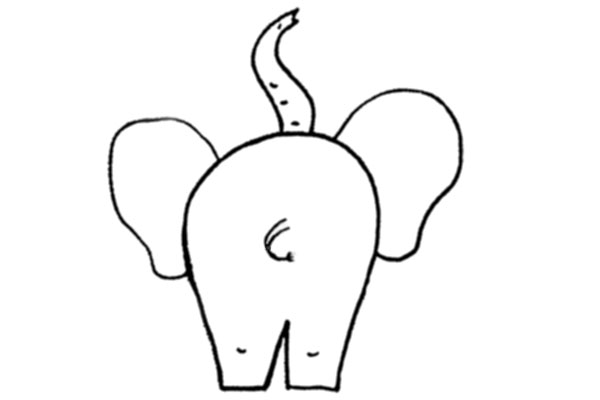
\includegraphics[scale=1.5]{images/slon.jpg}
\end{center}

\item
Укажите названия букв греческого алфавита и запишите соответствующие заглавные буквы:
\[\alpha, \zeta, \eta, \theta\].

\end{enumerate}



\newpage
\subsection[2014-2015]{\hyperref[sec:sol_kr_01_2014_2015]{2014-2015}}
\label{sec:kr_01_2014_2015}

\begin{enumerate}
\item Вася забыл какую-то (какую?) формулу. Он помнит, что она начинается
с «$\P(A|B) = $». Дальше была дробь, три буквы $\P$ со скобками после них и
в сумме по две буквы $A$ и $B$ внутри этих скобок. Ещё там была вертикальная черта «|».
Из этих элементов Вася случайным образом составляет формулу.
\begin{enumerate}
\item С какой вероятностью Вася напишет правильную формулу?
\item Напишите формулу, которую забыл Вася.
\end{enumerate}

Примечание: Вася всё-таки успел сходить на пару лекций по теории вероятностей и помнит,
что $\P(A|B)$ и $\P(B|A)$ — это не одно и то же, «|» должна стоять именно между буквами
(то ли $A|B$, то ли $B|A$), а в скобках, которые идут после $\P$, должно хоть что-то стоять.
При этом формула должна иметь смысл, то есть  $\P(A|B)$   не должна выражаться через себя же,
и дробь не должна быть сократимой.

\item Точка с координатами $(\xi, \eta)$ бросается наудачу в треугольник с вершинами
$(1,0)$, $(0,0)$, $(0,1)$. Сформулируйте определение независимости двух событий и
проверьте, будут ли события $A=\{ \xi < 1/2 \}$  и $B=\{ \eta < 1/2 \}$  независимыми?

\item На учениях три самолёта одновременно и независимо атакуют цель.
Известно, что первый самолёт поражает цель с вероятностью $0.6$, второй — $0.4$,
третий — $0.3$. При разборе учений выяснилось, что цель была поражена только
одним самолётом. Какова вероятность того, что это был первый самолёт?

\item Книга в $500$ страниц содержит $400$ опечаток. Предположим, что каждая
из них независимо от остальных опечаток может с одинаковой вероятностью оказаться
на любой странице книги.
\begin{enumerate}
\item Определите вероятность того, что на $13$-й странице будет не менее двух опечаток,
в явном виде и с помощью приближения Пуассона.
\item Определите наиболее вероятное число, математическое ожидание и дисперсию числа
опечаток на $13$-ой странице.
\item Является ли $13$-ая страница более «несчастливой», чем все остальные
(в том смысле, что на $13$-ой странице ожидается большее количество очепяток,
чем на любой другой)?
\end{enumerate}

Подсказка. Можно считать, что опечатки «выбирают» любую из страниц для своего
появления независимо друг от друга. Успех заключается в выборе $13$-ой страницы.
Вероятность успеха?

\item Вероятность того, что медицинский тест выявит наличие заболевания,
когда оно действительно есть, называется чувствительностью теста. Специфичностью
теста называется вероятность того, что тест покажет отсутствие заболевания,
когда пациент здоров. Вероятность того, что пациент болен, когда тест показал
наличие заболевания, называется прогностической силой теста. Предположим, что
только 1\,\%  всего населения страдает данным заболеванием.  Чувствительность
используемого теста равна $0.9$, а специфичность — $0.95$.
\begin{enumerate}
\item Какова вероятность того, что у случайно выбранного человека тест покажет
наличие заболевания?
\item Какова прогностическая сила теста? Что нужно сделать, чтобы её повысить?
\end{enumerate}

\item Функция плотности случайной величины $X$ имеет вид:
\begin{equation*}
f(x) =
 \begin{cases}
   1.5 (x-a)^2 &, x \in [0,a]\\
   1.5 (x+a)^2 &, x \in [-a,0]\\
   0 &, x \not\in [-a,a]
 \end{cases}
\end{equation*}

\begin{enumerate}
\item Найдите константу $a$, вероятность попадания в отрезок $\left[1/2, 2 \right]$,
математическое ожидание $X$ и дисперсию случайной величины $X$.
\item Нарисуйте функцию распределения случайной величины $X$.
\end{enumerate}

\item Вася случайным образом посещает лекции по ОВП (Очень Важному Предмету).
С вероятностью $0.9$ произвольно выбранная лекция полезна, и с вероятностью $0.7$ она интересна.
Полезность и интересность — независимые друг от друга и от номера лекции свойства.
Всего Вася прослушал 30 лекций.
\begin{enumerate}
\item Определите математическое ожидание и дисперсию числа полезных лекций и
числа интересных лекций, прослушанных Васей.
\item Определите математическое ожидание числа бесполезных и неинтересных лекций,
прослушанных Васей, и числа лекций, обладающих хотя бы одним из свойств (полезность,
интересность).
\end{enumerate}

\item Пусть $\E(X) = 1$, $\E(Y) = 2$, $\E\left(X^2\right) = 5$, $\E(XY) = -1$. Найдите:
\begin{enumerate}
\item $\E(2X + Y - 4)$
\item $\Var(X)$, $\Var(Y)$
\item $\Cov(X,Y)$, $\Corr(X,Y)$
\item $\Var(X-Y-1)$,  $\Var(X+Y+1)$
\item $\Cov(X-Y-1, X+Y+1)$,  $\Corr(X-Y-1, X+Y+1)$
\end{enumerate}

\item Совместное распределение случайных величин $X$ и $Y$ задано в виде таблицы:

\begin{center}
\begin{tabular}{ccc}
\toprule
 & $X=1$ & $X=2$ \\ \midrule
$Y=-1$ & $0.1$ & $0.2$ \\
$Y=0$ & $0.2$ & $0.3$ \\
$Y=1$ & $0$ & $0.2$ \\ \bottomrule
\end{tabular}
\end{center}

\begin{enumerate}
\item Найти частные распределения $Y$ и $Y^2$
\item Найти ковариацию случайных величин $X$ и $Y$
\item Можно ли утверждать, что случайные величины зависимы?
\end{enumerate}

\item Бонусная задача

Какова вероятность того, что наугад выбранный ответ на этот вопрос окажется верным
(искомую вероятность вычислить и записать!)?
\begin{enumerate}
\item 0.25
\item 0.5
\item 0.6
\item 0.25
\end{enumerate}
\end{enumerate}



\newpage
\subsection[2013-2014]{\hyperref[sec:sol_kr_01_2013_2014]{2013-2014}}
\label{sec:kr_01_2013_2014}


\begin{enumerate}
\item Вероятность застать Васю на лекции зависит от того, пришли ли на лекцию Маша и Алена.
Данная вероятность равна $0.18$, если девушек нет; $0.9$ — если обе девушки пришли на лекцию;
$0.54$ — если пришла только Маша и $0.36$ — если пришла только Алена.
Маша и Алена посещают лекции независимо друг от друга с вероятностями $0.4$ и $0.6$ соответственно.
\begin{enumerate}
\item Определите вероятность того, что на лекции присутствует Алена, если в аудитории есть Вася.
\item Кого чаще можно застать на тех лекциях, на которых присутствует Вася: Машу или Алену?
%\item При каком значении $p$ Вася посещает половину всех лекций?
\end{enumerate}

\item Страховая компания страхует туристов, выезжающих за границу,
от невыезда и наступления страхового медицинского случая за границей.
Застраховано 100 туристов. Вероятность «невыезда» за границу случайно
выбранного туриста — $0.002$, а страховые выплаты в этом случае — 2000 у.е.;
вероятность обращения за медицинской помощью за границей — $0.01$,
а страховые выплаты — 3000 у.е. Для каждого туриста рассмотрим две случайные
величины: $X_i$, равную 1 при невыезде за границу и 0 иначе, и $Y_i$, равную 1
при обращении за медицинской помощью и нулю иначе.
Обозначим $X=\sum_{i=1}^{100}X_i$ и $Y=\sum_{i=1}^{100}Y_i$.
\begin{enumerate}
\item Определите $\P(X=5)$, $\E(X)$, $\Var(X)$.
\item Наиболее вероятное число не выехавших туристов.
\item Вычислите математическое ожидание и дисперсию величины совокупных страховых выплат.
\end{enumerate}
Подсказка: Число обращений в страховую компанию для каждого туриста может быть
записано в виде $X_i+X_i Y_i$, так как медицинский страховой случай может наступить
только, если турист выехал за границу. Случайные величины $X_i$ и $Y_i$ независимы.

\item Функция плотности случайной величины $X$ имеет вид:
\begin{equation}
f(x)=\begin{cases}
ce^{-x}, \, x\geq 0 \\
ce^x, \, x<0
\end{cases}
\end{equation}
\begin{enumerate}
\item Найдите $c$, $\P(X \in [\ln 0.5,\ln 4])$, $\E(X)$, $\Var(X)$
\item Моменты всех порядков случайной величины $x$
\end{enumerate}

Подсказка: $\int_0^{\infty} x^n e^{-x} \, dx=n!$

\item Известно, что  $\E(X)=-1$, $\E(Y)=1$, $\Var(X)=9$, $\Var(Y)=4$, $\Corr(X,Y)=1$.
Найдите
\begin{enumerate}
\item $\E(Y-2X-3)$, $\Var(Y-2X-3)$
\item  $\Corr(Y-2X-3,X)$
\item Можно ли выразить $Y$ через $X$? Если да, то запишите уравнение связи.
\end{enumerate}

\item Совместное распределение доходов акций двух компаний $Y$ и $X$ задано в виде таблицы

\begin{center}
\begin{tabular}{@{}cccc@{}}
\toprule
    & $X=-1$ & $X=0$ & $X=1$ \\ \midrule
$Y=-1$ & $0.1$  & $0.2$   & $0.2$ \\
$Y=1$ & $0.2$  & $0.1$ & $0.2$ \\ \bottomrule
\end{tabular}
\end{center}

\begin{enumerate}
\item Найдите  частные распределения случайных величин $X$ и $Y$
\item Найдите $\Cov(X,Y)$
\item Можно ли утверждать, что случайные величины $X$ и $Y$ зависимы?
\item Найдите условное распределение случайной величины $X$ при условии $Y=-1$
\item Найдите условное математическое ожидание $\E(X\mid Y=-1)$
\end{enumerate}
\end{enumerate}



\newpage
\subsection[2012-2013]{\hyperref[sec:sol_kr_01_2012_2013]{2012-2013}}
\label{sec:kr_01_2012_2013}


\begin{enumerate}

\item Погода завтра может быть ясной с вероятностью $0.3$ и пасмурной с вероятностью $0.7$.
Вне зависимости от того, какая будет погода, Маша даёт верный прогноз с вероятностью $0.8$.
Вовочка, не разбираясь в погоде, делает свой прогноз по принципу: с вероятностью $0.9$
копирует Машин прогноз, и с вероятностью $0.1$ меняет его на противоположный.
\begin{enumerate}
\item Какова вероятность того, что Маша спрогнозирует ясный день?
\item Какова вероятность того, что Машин и Вовочкин прогнозы совпадут?
\item Какова вероятность того, что день будет ясный, если Маша спрогнозировала ясный?
\item Какова вероятность того, что день будет ясный, если Вовочка спрогнозировал ясный?
\end{enumerate}

\item Машин результат за контрольную, $M$, равномерно распределен на отрезке $[0;1]$.
Вовочка ничего не знает, поэтому списывает у Маши, да ещё может наделать ошибок при
списывании. Поэтому Вовочкин результат, $V$, распределен равномерно от нуля до Машиного
результата.
\begin{enumerate}
\item Найдите $\P(M>2V)$, $\P(M>V+0.1)$
\item Зачёт получают те, чей результат больше $0.4$. Какова вероятность того, что Вовочка получит зачёт? Какова вероятность того, что Вовочка получит зачёт, если Маша получила зачёт?
\end{enumerate}
Подсказка: попробуйте нарисовать нужные события в осях $(V,M)$

Это была задачка-неберучка!

\item Функция плотности случайной величины $X$ имеет вид
\[
f(x)=
\begin{cases}
\frac{3}{7}x^2, & x\in[1;2] \\
0,& x \notin [1,2]
\end{cases}
\]
\begin{enumerate}
\item Не производя вычислений найдите $\int_{-\infty}^{+\infty}f(x)\,dx$
\item Найдите $\E(X)$, $\E(X^2)$ и дисперсию $\Var(X)$
\item Найдите $\P(X>1.5)$
\item Найдите функцию распределения $F(x)$ и постройте её график
\end{enumerate}

\item Совместное распределение случайных величин $X$ и $Y$ задано таблицей

\begin{center}
\begin{tabular}{@{}cccc@{}}
\toprule
      & $X=-2$ & $X=0$ & $X=2$ \\ \midrule
$Y=1$ & $0.2$  & $0.3$ & $0.1$ \\
$Y=2$ & $0.1$  & $0.2$ & $a$   \\ \bottomrule
\end{tabular}
\end{center}

\begin{enumerate}
\item Определите неизвестную вероятность $a$.
\item Найдите вероятности $\P(X>-1)$, $\P(X>Y)$
\item Найдите математические ожидания $\E(X)$, $\E\left(X^2\right)$
\item Найдите корреляцию $\Corr(X,Y)$
\end{enumerate}

\item Винни Пух собрался полакомиться медом, но ему необходимо принять решение,
к каким пчелам отправиться за медом. Неправильные пчелы кусают каждого, кто лезет
к ним на дерево с вероятностью $0.9$, но их всего 10 штук. Правильные пчелы кусаются
с вероятностью $0.1$, но их 100 штук.
\begin{enumerate}
\item  Определите математическое ожидание и дисперсию числа укусов Винни Пуха для каждого случая
\item Определите наиболее вероятное число укусов и его вероятность для каждого случая
\item К каким пчелам следует отправиться Винни Пуху, если он не может выдержать больше двух укусов?
\end{enumerate}
\end{enumerate}

\newpage
\thispagestyle{empty}
\section{Контрольная работа 1. ИП}

\subsection[2018-2019]{\hyperref[sec:sol_kr_01_ip_2018_2019]{2018-2019}}
\label{sec:kr_01_ip_2018_2019}

\begin{enumerate}
\item Пират Злопамятный Джо очень любит неразбавленный ром. Из-за того,
что он много пьёт, у него проблемы с памятью, и он помнит не больше,
чем три последних пинты. Хозяин таверны «Огненная зебра»
с вероятностью $1/8$ разбавляет каждую подаваемую пинту рома.
Если по ощущением Джо половина выпитых пинт или больше была разбавлена, то он
разносит таверну к чертям собачьим.
Только что Джо вошёл в таверну и закал первую пинту.

Сколько в среднем пинт выпьет Джо, прежде чем разнесёт таверну?

\item В таверне «Крутой ковбой» разбавленный ром подают с вероятностью $1/2$.
Джо немного сменил свой характер и теперь устраивает скандал,
если две пинты рома подряд разбавлены.

Какова вероятность того, что Джо сможет выпить 100 пинт подряд без скандалов?

\item Али-Баба хочет проникнуть в пещеру с сокровищами. Вход в
пещеру закрыт и его охраняет Джин с квадратным подносом.
В каждой вершине подноса — непрозрачный стаканчик. Под
каждым стаканчиком — монетка.
Если все четыре монетки окажутся в одинаковом положении, все —
орлом вверх, или все — решкой вверх, то вход откроется.
За одно действие Али-Баба может открыть любые два стаканчика и
положить открывшиеся монетки любой стороной вверх.
После действия Али-Бабы Джин накрывает монетки стаканчиками,
быстро-быстро вращает поднос и снова предоставляет поднос
Али-Бабе.
Углядеть за Джином или сделать пометки на подносе невозможно.

\begin{enumerate}
  \item Как надо действовать Али-Бабе, чтобы гарантировать себе вход в
  пещеру за наименьшее количество действий?
  \item Сколько действий
  потребуется в худшем случае?
\end{enumerate}

\item Злопамятный Джо очень любит играть в картишки. Перед Джо хорошо перемешанная
стандартная колода в 52 карты. Джо извлекает карты по одной.

На каком месте в среднем появляется первая Дама?

\item Вероятность того, что непросветлённый Ученик достигнет Просветления за малый интервал времени,
прямо пропорциональна длине этого интервала, а именно,
\[
\P(\text{достигнуть Просветления за отрезок времени }[t;t+\Delta]) =
0.2018 \Delta + o(\Delta)
\]

Какова точная вероятность того, что Ученик, начавший искать Просветление, так
и не достигнет его к моменту времени $t$?

\item Исследователь Василий выбирает равномерно и независимо друг от друга 10 точек на
отрезке $[0;1]$. Затем Василий записывает их координаты в порядке возрастания,
$Y_1 \leq Y_2 \leq \ldots \leq Y_{10}$.

Не производя вычислений, \textit{по определению},
выпишите функции плотности случайной величины $Y_4$.
\end{enumerate}


\newpage

\subsection[2017-2018]{\hyperref[sec:sol_kr_01_ip_2017_2018]{2017-2018}}
\label{sec:kr_01_ip_2017_2018}

Ровно 272 года назад императрица Елизавета повелела завезти во дворцы котов для ловли мышей.

\begin{enumerate}
\item В отсутствии кота Леопольда мыши Белый и Серый подкидывают по очереди
игральный додекаэдр.
%\footnote{Леопольд подсказывает по случаю праздника, что у додекаэдра 12 граней :)}
Сыр достаётся тому, кто первым выкинет число 6. Начинает подкидывать Белый.
\begin{enumerate}
  \item Какова вероятность того, что сыр достанется Белому?
  \item Сколько в среднем бросков продолжается игра?
  \item Какова дисперсия числа бросков?
\end{enumerate}

\item Микки Маус, Белый и Серый решили устроить труэль из любви к мышки Мии.
Сначала делает свой выстрел Микки, затем Белый, затем Серый, затем снова Микки и так до тех пор,
пока в живых не останется только один.

Прошлые данные говорят о том, что Микки попадает с вероятностью $1/3$,
Белый — с вероятностью $2/3$, а Серый стреляет без промаха.

Найдите оптимальную стратегию каждого мыша, куда кому следует целиться.

\item Микки Маус, Белый и Серый пойманый злобным котом Леопольдом до начала труэли.
И теперь Леопольд будет играть с ними в странную игру.

В комнате три закрытых внешне неотличимых коробки: с золотом, серебром и платиной.
Общаться после начала игры мыши не могут, но могут заранее договориться о стратегии.

Правила игры таковы. Кот Леопольд будет заводить мышей в комнату по очереди.
Каждый из мышей может открыть две коробки по своему выбору.
Перед следующим мышом коробки закрываются.

Если Микки откроет коробку с золотом, Белый — с серебром, а Серый — с платиной,
то они выигрывают. Если хотя бы один из мышей не найдёт свой металл, то Леопольд
их съест.
\begin{enumerate}
\item Какова оптимальная стратегия?
\item Какова вероятность выигрыша при использовании оптимальной стратегии?
\end{enumerate}

\item Накануне войны Жестокий Тиран Мышь очень большой страны издал указ.
Отныне за каждого новорождённого мыша-мальчика семья получает денежную премию,
но если в семье рождается вторая мышка-девочка, то всю семью убивают.
Бедные жители страны запуганы и остро нуждаются в деньгах, поэтому в каждой семье
мыши будут появляться до тех пор, пока не родится первая мышка-девочка.
\begin{enumerate}
  \item Каким будет среднее число детей в мышиной семье?
  \item Какой будет доля мышей-мальчиков в стране?
  \item Какой будет средняя доля мышей-мальчиков в случайной семье?
  \item Сколько в среднем мышей-мальчиков в случайно выбираемой семье?
\end{enumerate}

\item Вальяжный кот Василий положил на счёт в банке на Гаити один гурд.
Сумма на счету растёт непрерывно с постоянной ставкой в течение очень длительного
промежутка времени. В случайный момент этого промежутка кот Василий закрывает свой вклад.

Каков закон распределения первой цифры полученной Василием суммы?
\end{enumerate}



\newpage
\subsection[2016-2017]{\hyperref[sec:sol_kr_01_ip_2016_2017]{2016-2017}}
\label{sec:kr_01_ip_2016_2017}


\begin{enumerate}
\item Задача о макаронинах

В тарелке запутавшись лежат много-много макаронин.
Я по очереди связываю попарно все торчащие концы макаронин.
\begin{enumerate}
\item Какова примерно вероятность того, что я свяжу все макаронины в одно большое кольцо?
\item Сколько в среднем колец образуется?
\item Каково среднее число колец длиной в одну макаронину?
\end{enumerate}

\item Планета Плюк

На планету Плюк, окружность, в случайных точках садятся $n$ пепелацев.
Радиосвязь между двумя точками на планете Плюк возможна, если центральный угол
между этими двумя точками меньше $\pi/2$.
\begin{enumerate}
\item Какова вероятность того, что из любой точки планеты можно связаться хотя бы с одним пепелацем?
\item Какова вероятность того, что при $n=3$ все три пепелаца смогут поддерживать связь друг с другом (необязательно напрямую, возможно через посредника)?
\item Как изменятся ответы, если планета Плюк — это сфера?
\end{enumerate}

\item Чайник Рассела

Вокруг Солнца по эллиптической орбите вращается абсолютно плоский чайник Рассела
с площадью $42$ см$^2$. Летающий Макаронный Монстр проецирует чайник Рассела на
случайную плоскость.

Чему равна ожидаемая площадь проекции?

% \item Винни-Пух собирается играть в Пустяки и готовит для игры палочки. Он нашел
% палку длиной 1 м, а дальше поступает следующим образом. Разламывает палку равномерно
% в случайном месте, одну полученную часть использует для игры, а вторую снова случайным
% образом делит на две части. Далее одну новую часть Винни-Пух снова использует
% для игры, а вторую новую часть снова делит на две. И так далее. Обозначим $X_i$ —
% длину палочки, использованной Винни-Пухом в $i$-ых Пустяках.

% Найдите функцию плотности $X_i$, $\E(X_i)$, $\Var(X_i)$

\item Чак Норрис против Брюса Ли

Чак Норрис хватается за верёвку в форме окружности в произвольной точке.
Брюс Ли берёт мачете и с завязанными глазами разрубает верёвку в двух случайных
независимых местах. Чак Норрис забирает себе тот кусок, за который держится.
Брюс Ли забирает оставшийся кусок.  Вся верёвка имеет единичную длину.
\begin{enumerate}
\item Чему равна ожидаемая длина куска верёвки, доставшегося Брюсу Ли?
\item  Вероятность того, что у Брюса Ли верёвка длиннее?
\end{enumerate}

\item Истеричная певица

Начинающая певица дает концерты каждый день. Каждый её концерт приносит продюсеру
$0.75$ тысяч евро. После каждого концерта певица может впасть в депрессию
с вероятностью $0.5$. Самостоятельно выйти из депрессии певица не может.
В депрессии она не в состоянии проводить концерты. Помочь ей могут только хризантемы
от продюсера. Если подарить цветы на сумму $0\le x\le 1$ тысяч евро, то она выйдет
из депрессии с вероятностью $\sqrt{x}$.

Какова оптимальная стратегия продюсера, максимизирующего ожидаемую прибыль?

\item Гадалка

Джульетта пишет на бумажках два любых различных натуральных числа по своему выбору.
Одну бумажку она прячет в левую руку, а другую — в правую. Ромео выбирает любую руку
Джульетты. Джульетта показывает число, написанное на выбранной бумажке. Ромео высказывает
свою догадку о том, открыл ли он большее из двух чисел или меньшее. Ромео выигрывает,
если он угадал.

Приведите пример стратегии Ромео, дающей ему вероятность выигрыша строго больше
$0.5$ против любой стратегии Джульетты.

\item Мудрецы

В ряд друг за другом за бесконечным столом сидит счётное количество Мудрецов,
постигающих Истину. Первым сидит Абу Али Хусейн ибн Абдуллах ибн аль-Хасан ибн
Али ибн Сина:

\begin{figure}[h!]
  \begin{center}
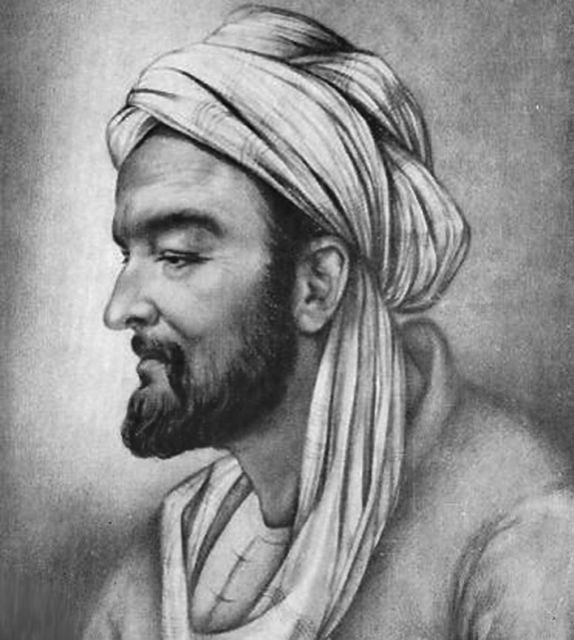
\includegraphics[width=5cm]{images/abu_ali.jpg}
  \caption*{«Коль смолоду избрал к заветной правде путь, \\
 С невеждами не спорь, советы их забудь». }
 \end{center}
\end{figure}

Каждый Мудрец может постигнуть Истину самостоятельно с вероятностью $1/9$
или же от соседа\footnote{Студенты постигают Истину примерно также!}. Независимо
от способа постижения Истины, просветлённый Мудрец поделится Истиной с соседом
слева с вероятностью $2/9$ и с соседом справа также с вероятностью $2/9$ (независимо
от соседа слева).
\begin{enumerate}
\item Какова вероятность того, что Абу Али Хусейн ибн Абдуллах ибн аль-Хасан ибн
Али ибн Сина постигнет Истину?
\item Как изменится ответ, если ряд Мудрецов бесконечен в обе стороны?
\end{enumerate}
\end{enumerate}



\newpage
\subsection[2015-2016]{\hyperref[sec:sol_kr_01_ip_2015_2016]{2015-2016}}
\label{sec:kr_01_ip_2015_2016}

\subsubsection*{Индивидуальный тур}

\begin{enumerate}
\item Для разминки вспомним греческий алфавит!

\begin{enumerate}
\item По-гречески — Σωκρατης, а по-русски — \underline{\hspace{2cm}}
\item Изобразите прописные и строчные буквы: эта \underline{\hspace{2cm}},
дзета \underline{\hspace{2cm}}, вега \underline{\hspace{2cm}},
шо \underline{\hspace{2cm}}. Если такой буквы в греческом нет, то поставьте прочерк.
\item Назовите буквы: τ \underline{\hspace{2cm}}, θ \underline{\hspace{2cm}},
ξ \underline{\hspace{2cm}}.
%\item Если пересчитать все буквы в греческом алфавите, то их окажется ровно \underline{\hspace{2cm}} %24
\end{enumerate}

\item Подбрасываются 2 симметричные монеты. Событие $A$ — на первой монете выпал герб,
событие $B$ — на второй монете выпал герб, событие $C$ — монеты выпали разными сторонами.
\begin{enumerate}
\item Будут ли эти события попарно независимы?
\item Сформулируйте определение независимости в совокупности для трех событий
\item Являются ли события $A$, $B$, $C$ независимыми в совокупности?
\end{enumerate}


\item Имеются два игральных кубика: \textbf{красный} со смещенным центром тяжести,
так что вероятность выпадения «6» равняется $1/3$, а оставшиеся грани имеют равные
шансы на появление и
правильный \textbf{белый} кубик.  Петя случайным образом выбирает кубик и подбрасывает его.
\begin{enumerate}
\item Вероятность того, что выпадет «6», равна \underline{\hspace{2cm}}
\item Вероятность того, что Петя взял красный кубик, если известно, что выпала шестерка,
равна \underline{\hspace{2cm}}
\item Если бы в эксперименте Петя подбрасывал  бы кубик не один раз, а 60 раз,
то безусловное математическое ожидание количества выпавших шестёрок равнялось бы
\underline{\hspace{2cm}}
\end{enumerate}

\begin{comment}
\item Неразменный пятак всегда выпадает «орлом». У Александра Привалова в кармане
один неразменный пятак и два обычных, равновероятно выпадающих «орлом» и «решкой».
Привалов достаёт одну из монет наугад не глядя.
\begin{enumerate}
\item Вероятность того, что он достанет неразменный пятак равна \underline{\hspace{2cm}} % 1/3
\item Не глядя на монету, Привалов подкидывает её. Вероятность того, что она выпадет
«орлом», равна \underline{\hspace{2cm}} % 2/3
%\item Если бы эту случайную монету подкинуть не один раз, а 10, то математическое ожидание числа «орлов» равнялось бы \underline{\hspace{2cm}} % 20/3
\item Наконец Привалов глядит на упавшую монету и видит, что выпал «орёл».
Вероятность того, что монета — неразменный пятак, равна \underline{\hspace{2cm}}
\end{enumerate}
\end{comment}

\item Винни-Пуху снится сон, будто он спустился в погреб, а там бесконечное
количество горшков. Каждый из них независимо от других может оказаться либо
пустым с вероятностью $0.8$, либо с мёдом с вероятностью $0.2$. Винни-Пух начинает
перебирать горшки по очереди в поисках полного. Хотя у него в голове и опилки,
Винни-Пух два раза в один и тот же горшок заглядывать не будет.
\begin{enumerate}
\item Вероятность того, что все горшки окажутся пустыми равна \underline{\hspace{2cm}}
\item Вероятность того, что полный горшок будет найден ровно с шестой попытки, равна \underline{\hspace{2cm}}
\item Вероятность того, что полный горшок будет найден на шестой попытке или ранее, равна \underline{\hspace{2cm}}
%\item Математическое ожидание числа перебранных горшков равняется \underline{\hspace{2cm}} % 5
\end{enumerate}

\item На самом деле у Винни-Пуха в погребе стоит 10 горшков. Каждый из них независимо
от других может оказаться либо пустым с вероятностью $0.8$, либо с мёдом с вероятностью
$0.2$.
\begin{enumerate}
\item Все десять горшков окажутся пустыми с вероятностью \underline{\hspace{2cm}}
\item Ровно $7$ горшков из десяти окажутся пустыми с вероятностью \underline{\hspace{2cm}}
\item Математическое ожидание числа горшков с мёдом равно \underline{\hspace{2cm}}
\end{enumerate}


\begin{comment}
\item Внутри треугольника с вершинами $(0,0)$, $(2,5)$ и $(8,0)$ случайно
равномерно по площади выбирается точка. Пусть $X$ и $Y$ — абсцисса и ордината
этой случаной точки.
\begin{enumerate}
\item Вероятность того, что $X>5$ равна \underline{\hspace{2cm}}.
\item Вероятность того, что $X>5$ и одновременно $Y<3$ равна \underline{\hspace{2cm}}.
\item Вероятность того, что $X>5$ если известно, что $Y<3$ равна \underline{\hspace{2cm}}.
\item События $X>5$ и $Y<3$ являются \underline{\hspace{1cm}}висимыми.
\item Функция плотности величины $X$ равна \underline{\hspace{2cm}}
\end{enumerate}
\end{comment}

\item В галактике Флатландии все объекты двумерные. На планету Тау-Слона (окружность)
в случайных точках независимо друг от друга садятся три корабля. Любые два корабля
могут поддерживать прямую связь между собой, если центральный угол между ними меньше
прямого.
\begin{enumerate}
\item Вероятность того, что первый и второй корабли могут поддерживать прямую
связь равна \underline{\hspace{2cm}}
\item Вероятность того, что все корабли смогут поддерживать прямую связь друг
с другом равна \underline{\hspace{2cm}}
\item Вероятность того, что все корабли смогут поддерживать прямую связь друг
с другом, если первый и второй корабль могут поддерживать прямую связь, равна
\underline{\hspace{2cm}}
\end{enumerate}
Подсказка: во Флатландии хватит рисунка на плоскости, ведь координату третьего
корабля можно принять за\ldots

\item Время (в часах), за которое студенты выполняют экзаменационное задание
является случайной величиной $X$ с функцией плотности
\[
f(x)=\begin{cases}
3x^2, \, \text{ если } x \in [0;1] \\
0, \, \text{ иначе }
\end{cases}
\]

\begin{enumerate}
\item Функция распределения случайной величины $X$ равна \underline{\hspace{2cm}}
\item Вероятность того, что случайно выбранный студент закончит работу менее чем
за полчаса равна \underline{\hspace{2cm}}.
\item Медиана распределения равна \underline{\hspace{2cm}}
\item Вероятность того, что студент, которому требуется по меньшей мере 15 минут
для выполнения задания, справится с ним более, чем за 30 минут, равна \underline{\hspace{2cm}}
\item Функция распределения случайной величины $Y=1/X$ равна \underline{\hspace{2cm}}
\item Функция плотности случайной величины $Y=1/X$ равна \underline{\hspace{2cm}}
\end{enumerate}
\end{enumerate}

\subsubsection*{Командный тур}

\begin{enumerate}
\item Восьминогий Кракен. У Кракена 8 ног-шупалец. Если отрубить одно щупальце,
то в замен него с вероятностью $1/4$ вырастает новое; с вероятностью $1/4$ вырастает
два новых; с вероятностью $1/2$, слава Океану, не вырастает ничего.

Против Кракена бьётся сам Капитан! Он наносит точные удары и безупречно умело
уворачивается от ударов Кракена.
\begin{enumerate}
\item Какова вероятность того, что Капитан победит, отрубив ровно 10 щупалец?
\item Какова вероятность того, что бой Кракена и Капитана продлится вечно?
\item Сколько щупалец в среднем отрубит Капитан прежде чем победит?
\end{enumerate}

\item Разбавленный ром. Пират Злопамятный Джо очень любит неразбавленный ром. Из-за
того, что он много пьёт, у него проблемы с памятью, и он помнит не
больше, чем три последних пинты. Хозяин таверны с вероятностью $1/4$ разбавляет
каждую подаваемую пинту рома. Если по ощущением Джо половина выпитых
пинт или больше была разбавлена, то он разносит таверну к чертям собачьим.
\begin{enumerate}
\item Какова вероятность того, что хозяин таверны не успеет подать Джо третью пинту рома?
\item Сколько в среднем пинт выпьет Джо, прежде чем разнесёт таверну?
\end{enumerate}

\item $XY$ в степени $Z$. Чтобы поступить на службу Её Величества, пиратам предлагается
следующая задача. Случайные величины $X$, $Y$ и $Z$ равномерны на отрезке $[0;1]$
и независимы.
\begin{enumerate}
\item Найдите функцию распределения случайной величины $-\ln X$
\item Найдите функцию распределения случайной величины $-(\ln X + \ln Y)$
\item Найдите функцию распределения случайной величины $-Z(\ln X + \ln Y)$
\item Какое распределение имеет случайная величина $(XY)^Z$?
\end{enumerate}

\item Тортики. Пираты очень любят тортики и праздновать день рождения! Если хотя
бы у одного пирата на корабле день рождения, то все, включая капитана, празднуют
и кушают тортики. Корабль в праздничный день дрейфует под действием ветра и не факт,
что в нужном направлении.
\begin{enumerate}
\item Сколько пиратов нужно нанять капитану, чтобы ожидаемое количество праздничных
дней было равно 100?
\item Сколько пиратов нужно нанять капитану, чтобы максимизировать ожидаемое количество
рабочих пирато-дней (произведение числа пиратов на число рабочих дней)?
\end{enumerate}

\item Девятый вал. На побережье пиратского острова одна за одной набегают волны.
Высота каждой волны — равномерная на $[0;1]$ случайная величина. Высоты волн независимы.
Пираты называют волну «большой», если она больше предыдущей и больше следующей.
Пираты называют волну «рекордной», если она больше всех предыдущих волн от начала
наблюдения. Обозначим события $B_i= \{ i\text{-ая волна была большой} \}$ и
$R_i=\{ i\text{-ая волна была рекордной} \}$.
\begin{enumerate}
\item Найдите $\P(R_{100})$, $\P(B_{100})$
\item Капитан насчитал 100 волн. Сколько в среднем из них были «рекордными»?
\item Найдите $\P(R_{99} | R_{100})$, $\P(R_{100}|B_{100})$
\end{enumerate}

\item Три сундука. Три пирата, Генри Рубинов, Френсис Пиастров и Эдвард Золотов
играют одной командой в игру. В комнате в ряд, слева направо, стоят в случайном
порядке три закрытых внешне неотличимых сундука: с рубинами, пиастрами и золотом.
Общаться после начала игры они не могут, но могут заранее договориться о стратегии.
Они заходят в комнату по очереди. Каждый из них может открыть два сундука по своему
выбору. После каждого пирата комната возвращается уборщицей идеально точно в исходное
состояние. Если Рубинов откроет коробку с рубинами, Писатров — с пиастрами, а Золотов —
с золотом, то их команда выигрывает. Если хотя бы один из пиратов не найдёт свою цель,
то их команда проигрывает.
\begin{enumerate}
\item Какова вероятность выигрыша, если все пираты пробуют открыть первый и второй сундуки?
\item Какова оптимальная стратегия?
\item Какова вероятность выигрыша при использовании оптимальной стратегии?
\end{enumerate}
\end{enumerate}


\newpage
\subsection[2014-2015]{\hyperref[sec:sol_kr_01_ip_2014_2015]{2014-2015}}
\label{sec:kr_01_ip_2014_2015}

\subsubsection*{ Часть 1}

\begin{enumerate}
%\item Винни-Пух собирается играть в Пустяки и готовит для игры палочки. Он нашел палку длиной 1 м, а дальше поступает следующим образом. Разламывает палку равномерно в случайном месте, одну полученную часть использует для игры, а вторую снова случайным образом делит на две части. Далее одну новую часть Винни-Пух снова использует для игры, а вторую новую часть снова делит на две. И так далее. Обозначим $X_i$ — длину палочки, использованной Винни-Пухом в $i$-ых Пустяках.

%Найдите функцию плотности $X_i$, $\E(X_i)$, $\Var(X_i)$

\item Вася купил два арбуза у торговки тёти Маши и один арбуз у торговки тёти Оли.
Арбузы у тёти Маши спелые с вероятностью 90\% (независимо друг от друга), арбузы
у тёти Оли спелые с вероятностью 70\%.
\begin{enumerate}
\item Какова вероятность того, что все Васины арбузы спелые?
\item Придя домой Вася выбрал случайным образом один из трех арбузов и разрезал его.
Какова вероятность того, что это арбуз от тёти Маши, если он оказался спелым?
\item Какова вероятность того, что второй и третий съеденные Васей арбузы были от
тёти Маши, если все три арбуза оказались спелыми?
\end{enumerate}


\item В большой большой стране живет очень большое количество $n$ семей.
Количества детей в разных семьях независимы. Количество детей в каждой семье —
случайная величина с распределением заданным табличкой:

\begin{center}
\begin{tabular}{ccccc}
\toprule
$x$ & $0$ & $1$ & $2$ & $3$ \\ \midrule
$\P(X=x)$ & $0.1$ & $0.3$ & $0.2$ & $0.4$ \\ \bottomrule
\end{tabular}
\end{center}

\begin{enumerate}
\item Исследователь Афанасий выбирает одну семью из всех семей наугад, пусть $X$ —
число детей в этой семье. Найдите $\E(X)$ и $\Var(X)$.
\item Исследователь Бенедикт выбирает одного ребенка из всех детей наугад, пусть $Y$ —
число детей в семье этого ребёнка. Как распределена величина $Y$? Что больше,
$\E(Y)$ или $\E(X)$?
\end{enumerate}

\item Функция плотности случайной величины $X$ имеет вид
\[
f(x)=
\begin{cases}
\frac{3}{8} x^2, \text{ если } x\in [0;2] \\
0, \text{ иначе }
\end{cases}
\]
\begin{enumerate}
\item Не производя вычислений найдите $\int_{-\infty}^{+\infty}f(x)\,dx$
\item Найдите $\E(X)$, $\E(X^2)$ и дисперсию $\Var(X)$
\item Найдите $\P(X>1.5)$, $\P(X>1.5 \mid X>1)$
\item При каком $c$ функция $g(x)=c x f(x)$ будет функцией плотности некоторой
случайной величины?
\end{enumerate}

\item Известно, что  $\E\left(Z\right)=-3$, $\E\left(Z^{2} \right)=15$,
$\Var\left(X+Y\right)=20$  и  $\Var\left(X-Y\right)=10$.
\begin{enumerate}
\item Найдите $\Var\left(Z\right)$, $\Var\left(4-3Z\right)$ и
$\E\left(5+3Z-Z^{2} \right)$.
\item Найдите $\Cov\left(X,Y\right)$ и $\Cov\left(6-X,3Y\right)$.
\item Можно ли утверждать, что случайные величины $X$ и $Y$ независимы?
\end{enumerate}

\item Листая сборник задач по теории вероятностей Вася наткнулся на задачу:

\fbox{%
\parbox{15cm}{%
Какова вероятность того, что наугад выбранный ответ на этот вопрос окажется верным?

1) $0.25$		2) $0.5$		3) $0.6$		4) $0.25$ }
}

Чему же равна вероятность выбора верного ответа?

\item Книга в 500 страниц содержит 400 опечаток. Предположим, что каждая из них
независимо от остальных опечаток может с одинаковой вероятностью оказаться на любой
странице книги.
\begin{enumerate}
\item Определите вероятность того, что на 13-й странице будет не менее двух опечаток,
в явном виде и с помощью приближения Пуассона.
\item Определите наиболее вероятное число, математическое ожидание и дисперсию
числа опечаток на 13-ой странице.
\item Является ли 13-ая страница более «несчастливой», чем все остальные (в том
смысле, что на 13-ой странице ожидается большее количество очепяток, чем на любой другой)?
\end{enumerate}

\item Вася случайным образом посещает лекции по ОВП (Очень Важному Предмету).
С вероятностью $0.9$ произвольно выбранная лекция полезна, и с вероятностью $0.7$
она интересна. Полезность и интересность — независимые друг от друга и от номера
лекции свойства. Всего Вася прослушал 30 лекций.
\begin{enumerate}
\item Определите математическое ожидание и дисперсию числа полезных лекций,
прослушанных Васей
\item Определите математическое ожидание числа одновременно бесполезных и
неинтересных лекций, прослушанных Васей, и математическое ожидание числа лекций,
обладающих хотя бы одним из свойств (полезность, интересность).
\end{enumerate}
\item Функция распределения случайной величины X задана следующей формулой:
 \[
 F(x)=\frac{ae^x}{1+e^x}+b
 \]
Определите: константы $a$ и $b$, математическое ожидание и третий начальный
момент случайной величины $X$, медиану и моду распределения.

%\item Вы хотите приобрести некую фирму. Стоимость фирмы для ее нынешних владельцев — случайная величина, равномерно распределенная на отрезке $[0;1]$. Вы предлагаете владельцам продать ее за называемую Вами сумму. Владельцы либо соглашаются, либо нет. Если владельцы согласны, то Вы платите обещанную сумму и получаете фирму. Когда фирма переходит в Ваши руки, ее стоимость сразу возрастает на 20\%.

%\begin{enumerate}
%\item Чему равен Ваш ожидаемый выигрыш, если Вы предлагаете цену 0.5?
%\item Какова оптимальная предлагаемая цена?
%\end{enumerate}
\end{enumerate}

\subsubsection*{Часть 2}

\begin{enumerate}
\item Маша подкидывает кубик до тех пор, пока два последних броска в сумме не
дадут\footnote{Изначально вместо 12 задумывалось число 10, но  опечатка была
замечена поздно, поэтому решение приводится для 12.} 12. Обозначим случайные
величины: $N$ — количество бросков, а $S$ — сумма набранных за всю игру очков.
\begin{enumerate}
\item Найдите $\P(N=2)$, $\P(N=3)$
\item Найдите $\E(N)$, $\E(S)$, $\E(N^2)$
\item Пусть $X_N$ — результат последнего броска. Как распределена случайная
величина $X_N$?
\end{enumerate}


\item В столовую пришли 30 студентов и встали в очередь в случайном порядке.
Среди них есть Вовочка и Машенька. Пусть $V$ — это количество человек в очереди
перед Вовочкой, а $M\geq 0$ — количество человек между Вовочкой и Машенькой.
\begin{enumerate}
\item Найдите $\P(V=1)$, $\P(M=1)$, $\P(M=V)$
\item Найдите $\E(V)$, $\E(M)$, $\Var(M)$
\end{enumerate}

\item Польский математик Стефан Банах имел привычку носить в каждом из двух
карманов пальто по коробку спичек. Всякий раз, когда ему хотелось закурить трубку,
он выбирал наугад один из коробков и доставал из него спичку. Первоначально в каждом
коробке было по $n$ спичек. Но когда-то наступает момент, когда выбранный наугад
коробок оказывается пустым.
\begin{enumerate}
\item Какова вероятность того, что в другом коробке в этот момент осталось ровно
$k$ спичек?
\item Каково среднее количество спичек в другом коробке?
\end{enumerate}

\item Производитель чудо-юдо-йогуртов наклеивает на каждую упаковку одну из 50
случайно выбираемых наклеек. Покупатель собравший все виды наклеек получает приз
от производителя. Пусть $X$ — это количество упаковок йогурта, которое нужно купить,
чтобы собрать все наклейки.

Найдите $\P(X=50)$, $\E(X)$, $\Var(X)$

Hint: $\ln(50)\approx 3.91$, а $\sum_{i=1}^n \frac{1}{i} \approx \int_1^n \frac{1}{x}\, dx$ :)

\item В самолете $n$ мест и все билеты проданы. Первой в очереди на посадку стоит
Сумасшедшая Старушка. Сумасшедшая Старушка несмотря на билет садиться на случайно
выбираемое место. Каждый оставшийся пассажир садится на своё место, если оно свободно
и на случайное выбираемое место, если его место уже кем-то занято.
\begin{enumerate}
\item Какова вероятность того, что все пассажиры сядут на свои места?
%\item Какова вероятность того, что второй пассажир в очереди сядет на своё место?
\item Какова вероятность того, что последний пассажир сядет на своё место?
\item Чему примерно равно среднее количество пассажиров севших на свои места?
\end{enumerate}
\end{enumerate}



\newpage
\subsection[2013-2014]{\hyperref[sec:sol_kr_01_ip_2013_2014]{2013-2014}}
\label{sec:kr_01_ip_2013_2014}

\subsubsection*{Часть 1}

\begin{enumerate}

\item В жюри три человека, они должны одобрить или не одобрить конкурсанта.
Два члена жюри независимо друг от друга одобряют конкурсанта с одинаковой
вероятностью $p$. Третий член жюри  для вынесения решения бросает правильную монету.
Окончательное решение выносится большинством голосов.
\begin{enumerate}
\item С какой вероятностью жюри одобрит конкурсанта?
\item Что выгоднее для  конкурсанта: чтобы решение принимало данное жюри, или
чтобы решение принимал один человек, одобряющий с вероятностью $p$?
\end{enumerate}

\item Вероятность застать Васю на лекции зависит от того, пришли ли на лекцию
Маша и Алена. Данная вероятность равна $p$, если девушек нет; $5p$ — если обе
девушки пришли на лекцию; $3p$ — если пришла только Маша и $2p$ — если пришла
только Алена. Маша и Алена посещают лекции независимо друг от друга с вероятностями
$0.6$ и $0.3$ соответственно.
\begin{enumerate}
\item Определите вероятность того, что на лекции присутствует Алёна,
если в аудитории есть Вася.
\item Кого чаще можно застать на тех лекциях, на которых присутствует Вася:
Машу или Алёну?
\item При каком значении $p$ Вася посещает половину всех лекций?
\end{enumerate}

\item Страховая компания страхует туристов, выезжающих за границу, от невыезда
и наступления страхового медицинского случая за границей. Застраховано 100 туристов.
Вероятность «невыезда» за границу случайно выбранного туриста — $0.002$,
а страховые выплаты в этом случае — 2000 у.е.; вероятность обращения за медицинской
помощью за границей — $0.01$, а страховые выплаты — 3000 у.е.
\begin{enumerate}
\item Определите вероятность того, что ровно пятеро туристов не смогут выехать за границу.
\item Найдите математическое ожидание, дисперсию и наиболее вероятное число не выехавших туристов.
\item Вычислите математическое ожидание и дисперсию величины совокупных страховых выплат
\item Вычислите ковариацию между выплатами по двум видам страхования.
\end{enumerate}

\item Известно, что  $\E(X)=-1$, $\E(Y)=1$, $\Var(X)=9$, $\Var(Y)=4$, $\Corr(X,Y)=1$.
Найдите
\begin{enumerate}
\item $\E(Y-2X-3)$, $\Var(Y-2X-3)$
\item  $\Corr(Y-2X-3,X)$
\item Можно ли выразить $Y$ через $X$? Если да, то запишите уравнение связи.
\end{enumerate}

\item Совместное распределение доходов акций двух компаний $Y$ и $X$ задано в виде
таблицы
\begin{center}
\begin{tabular}{@{}cccc@{}}
\toprule
    & $X=-1$ & $X=0$ & $X=1$ \\ \midrule
$Y=-1$ & $0.1$  & $0.2$   & $0.2$ \\
$Y=1$ & $0.2$  & $0.1$ & $0.2$ \\ \bottomrule
\end{tabular}
\end{center}

Найдите:
\begin{enumerate}
\item Частные распределения случайных величин $X$ и $Y$
\item $\Cov(X,Y)$
\item Можно ли утверждать, что случайные величины $X$ и $Y$ зависимы?
\item У инвестора портфель, в котором доля акций $X$ составляет $\alpha$,
а доля акций $Y$ — $(1-\alpha)$. Каковы должны быть доли, чтобы риск портфеля
(дисперсия дохода) был бы минимальным?
\item Условное распределение случайной величины $X$ при условии $Y=-1$.
\item Условное математическое ожидание $\E(X\mid Y=-1)$
\end{enumerate}
\item Докажите, что из сходимости в среднем порядка $s>0$ следует сходимость
по вероятности.
\end{enumerate}


\subsubsection*{Часть 2}

\begin{enumerate}
\item Муравей находится внутри спичечного коробка, в вершине $A$. В противоположной
вершине $B$ есть маленькая дырочка, через которую муравей сможет выбраться на поверхность.
В вершине $C$, соседней с вершиной $A$, лежит крупинка сахара. Муравей ползает
только по рёбрам коробка, выбирая каждый раз равновероятно одно из доступных в
вершине рёбер наугад. Например, он может поползти обратно.
\begin{enumerate}
\item Какова вероятность того, что муравей найдет крупинку сахара до того, как выберется?
\item Сколько в среднем перемещений понадобится муравью, чтобы выбраться?
\item Какова дисперсия количества перемещений, которые понадобятся муравью, чтобы
выбраться?
\end{enumerate}

\item В очереди стояло $20$ человек, когда касса внезапно закрылась. Поэтому $10$
случайных людей из очереди решили покинуть очередь. В результате этого очередь
оказалась разбита на случайное число кусков $X$. Найдите $\E(X)$, $\Var(X)$.

\item Предположим, что три возможных генотипа \verb|aa|, \verb|Aa| и \verb|AA|
изначально встречаются с частотами $p_1$, $p_2$ и $p_3$, где $p_1 + p_2 + p_3 = 1$.
Ген не сцеплен с полом, поэтому частоты $p_1$, $p_2$ и $p_3$ одинаковы для мужчин
и для женщин.
\begin{enumerate}
\item У семейных пар из этой популяции рождаются дети. Назовём этих детей первым
поколением. Каковы частоты для трёх возможных генотипов в первом поколении?
\item У семейных пар первого поколения тоже рождаются дети. Назовём этих детей
вторым поколением. Каковы частоты для трёх возможных генотипов во втором поколении?
\item Каковы частоты для трёх возможных генотипов в $n$-ном поколении?
\item Заметив явную особенность предыдущего ответа сформулируйте теорему о равновесии
Харди-Вайнберга. Прокомментируйте утверждение: «Любой рецессивный ген со временем
исчезнет».
\end{enumerate}

\item Световая волна может быть разложена на две поляризованные составляющие,
вертикальную и горизонтальную. Поэтому состояние отдельного поляризованного фотона
может быть описано\footnote{На самом деле внутренний мир фотона гораздо разнообразнее.}
углом $\alpha$. Поляризационный фильтр описывается углом поворота $\theta$. Фотон
в состоянии $\alpha$ задерживается поляризационным фильтром с параметром $\theta$
с вероятностью $p=\sin^2(\alpha-\theta)$ или проходит сквозь фильтр с вероятностью
$1 - p$, переходя при этом в состояние $\theta$.

\begin{enumerate}
\item Какова вероятность того, что поляризованный фотон в состоянии $\alpha$ пройдёт
сквозь фильтр с параметром $\theta=0$?
\item Имеется два фильтра и поляризованный фотон в состоянии $\alpha$. Первый
фильтр — с $\theta=0$, второй — c $\theta=\pi/2$. Какова вероятность того, что
фотон пройдет через оба фильтра?
\item Имеется три фильтра и поляризованный фотон в состоянии $\alpha$. Первый
фильтр — с $\theta=0$, второй — c $\theta=\beta$, третий — с $\theta=\pi/2$.
Какова вероятность того, что фотон пройдет через все три фильтра? При каких $\alpha$
и $\beta$ она будет максимальной и чему при этом она будет равна?
\item Объясните следующий фокус. Фокусник берет два специальных стекла и видно,
что свет сквозь них не проходит. Фокусник ставит между двумя стёклами третье, и
свет начинает проходить через три стекла.
\end{enumerate}
\end{enumerate}

\clearpage
\thispagestyle{empty}
\section{Контрольная работа 2}



\subsection[2017-2018]{\hyperref[sec:sol_kr_02_2017_2018]{2017-2018}}
\label{sec:kr_02_2017_2018}

\subsubsection*{Минимум}
% 2 + 4 + 14 + 16

\begin{enumerate}
\item Приведите определение условной вероятности случайного события, формулу Байеса.
\item Сформулируйте определение и свойства функции плотности случайной величины.
\item Сформулируйте определение  условного математического ожидания $\E(Y|X=x)$ для совместного дискретного и совместного абсолютно непрерывного распределений.
\item Сформулируйте неравенство Чебышёва и неравенство Маркова.

\item Задана таблица совместного распределения случайных величин $X$ и $Y$.
\begin{center}
\begin{tabular}{lccc}
\toprule
                       & $Y=-1$  & $Y=0$   & $Y=1$   \\
 \midrule
$X=0$                 & $0.2$ & $0.1$ & $0.3$ \\
 $X=1$                 & $0.2$ & $0.1$ & $0.1$ \\
 \bottomrule
\end{tabular}
\end{center}


\begin{enumerate}
    \item Найдите $F_{X,Y}(0, 0)$;
    \item Найдите $\E(X)$, $\E(X^2)$, $\E(Y)$, $\E(Y^2)$;
    \item Найдите $\Var(X)$, $\Var(Y)$;
    \item Найдите $\Cov(X, Y)$, $\Corr(X, Y)$
\end{enumerate}
\item Плотность распределения случайного вектора $(X,Y)$ имеет вид
\[
f_{X,Y}(x,y) =
\begin{cases}
\frac{4x+10y}{7}, & \text{при } (x,y) \in [0;1] \times [0;1] \\
0 , & \text{при } (x,y) \not\in [0;1] \times [0;1] \\
\end{cases}
\]

\begin{enumerate}
\item Найдите $\P(X \leq Y)$;
\item Найдите функцию плотности $f_X(x)$;
\item Найдите $\E(X)$, $\E(Y)$ и $\Cov(X, Y)$;
\item Являются ли случайные величины $X$ и $Y$ независимыми?
\end{enumerate}


\end{enumerate}

\subsubsection*{Задачи}

\begin{enumerate}[resume]

\item Статистика авиакомпании «А» за много лет свидетельствует о том, что 10\% людей, купивших билет на самолет, не являются на рейс. Авиакомпания продала 330 билетов на 300 мест.
\begin{enumerate}
\item Какова вероятность, что всем явившимся на рейс пассажирам хватит места?
\item Укажите наибольшее число билетов, которое можно продавать на 300 мест, чтобы случаи переполнения случались не чаще, чем на одном из десяти рейсов.
\end{enumerate}

\item Сегодня акция компании «Ух» стоит 1 рубль. Каждый день акция может с вероятностью 0.7 вырасти на 1\%, с вероятностью 0.2999 упасть на 1\% и с вероятностью 0.0001 обесцениться (упасть на 100\%).
\begin{enumerate}
\item Считая изменение цены акции независимыми, найдите математическое ожидание её стоимости через 20 торговых дней.
\item Найдите предел по вероятности среднего изменения цены акции в процентах на бесконечном промежутке времени (Ответ обоснуйте).
\item Найдите математическое ожидание цены акции на бесконечном промежутке времени.
\item Инвестор вложил все свои средства в акции компании «Ух». Найдите вероятность его разорения на бесконечном промежутке времени.
\end{enumerate}
\end{enumerate}


\newpage
\subsection[2016-2017]{\hyperref[sec:sol_kr_02_2016_2017]{2016-2017}}
\label{sec:kr_02_2016_2017}


\textbf{Неравенства Берри–Эссеена:} Для любых $n \in \mathbb{N}$ и всех $x \in \mathbb{R}$ имеет место оценка:
\[
    \bigl|F_{S_n^{*}}(x) - \Phi(x)\bigr| \leq 0.48 \cdot \frac{\E(|\xi_i - \E\xi_i|^3)}{\Var^{3/2}(\xi_i)\cdot\sqrt{n}} \text{,}
\]
где $\Phi(x) = \int_{-\infty}^{x}\frac{1}{\sqrt{2\pi}}e^{-\frac{t^2}{2}}\,dt$, \; $S_n^* = \frac{S_n - \E(S_n)}{\sqrt{\Var(S_n)}}$, \; $S_n = \xi_1 + \ldots + \xi_n$

\textbf{Распределение Пуассона:} Случайная величина $\xi$ имеет распределение Пуассона с параметром $\lambda > 0$,  если она принимает целые неотрицательные значения с вероятностями $\P(\{\xi = k\}) = \frac{\lambda^k}{k!}e^{-\lambda}$. Приличным студентам должно быть известно, что в этом случае $\E(\xi) = \Var(\xi) = \lambda$.

\begin{enumerate}
\item Пусть $\E(\xi) = 1$, $\E(\eta) = -2$, $\Var(\xi) = 1$, $\E(\eta^2) = 8$, $\E(\xi \eta) = -1$. Найдите
\begin{enumerate}
\item $\E(2\xi-\eta+1)$, $\Cov(\xi, \,\eta)$, $\Corr(\xi, \,\eta)$,  $\Var(2\xi-\eta+1)$;
\item $\Cov(\xi+\eta, \,\xi+1)$, $\Corr(\xi+\eta, \,\xi+1)$, $\Corr(\xi+\eta-24, \,365 - \xi - \eta)$, $\Cov(2016\cdot\xi, \, 2017)$.
\end{enumerate}

\item
Совместное распределение доходностей акций двух компаний задано с помощью таблицы:

\begin{center}
\begin{tabular}{ccc}
\toprule
         & $\eta=-1$ & $\eta=1$ \\
\midrule
$\xi=-1$  & $0.1$       & $0.2$   \\
$\xi=0$   & $0.2$       & $0.2$   \\
$\xi=2$   & $0.2$       & $0.1$   \\
\bottomrule
\end{tabular}
\end{center}

\begin{enumerate}
  \item Найдите частные распределения случайных величин $\xi$ и $\eta$.
  \item Найдите $\Cov(\xi,\,\eta)$.
  \item Сформулируйте определение независимости дискретных случайных величин.
  \item Являются ли случайные величины $\xi$ и $\eta$ независимыми?
  \item Найдите условное распределение случайной величины $\xi$, если $\eta = 1$.
  \item Найдите условное математическое ожидание случайной величины $\xi$, если $\eta = 1$.
  \item Найдите математическое ожидание и дисперсию величины $\pi = 0.5\, \xi + 0.5\, \eta$.
  \item Рассмотрим портфель, в котором $\alpha$ — доля акций с доходностью $\xi$ и $(1 - \alpha)$ — доля акций с доходностью $\eta$. Доходность этого портфеля есть случайная величина
  \[\pi(\alpha) = \alpha \xi + (1-\alpha)\eta.\]
  Найдите такую долю $\alpha \in [0;\,1]$, при которой доходность портфеля $\pi(\alpha)$ имеет наименьшую дисперсию.
\end{enumerate}

\item Число посетителей сайта \url{pokrovka11.wordpress.com} за один день имеет распределение Пуассона с математическим ожиданием 250.
\begin{enumerate}
  \item Сформулируйте неравенство Маркова. При помощи данного неравенства оцените вероятность того, что за один день сайт посетят более 500 человек.
  \item Сформулируйте неравенство Чебышева. Используя данное неравенство, определите наименьшее число дней, при котором с вероятностью не менее 99\% среднее за день число посетителей будет отличаться от 250 не~более чем на 10.
  \item Решите предыдущий пункт с помощью центральной предельной теоремы.
  \item Сформулируйте закон больших чисел. Обозначим через $\xi_i$ число посетителей сайта за $i$-ый день. Найдите предел по вероятности последовательности $\frac{\xi_1^2 + \ldots + \xi_n^2}{n}$ при $n \rightarrow \infty$.
\end{enumerate}

\item Отведав медовухи, Винни–Пух совершает случайное блуждание на прямой. Он стартует из начала координат и в каждую следующую минуту равновероятно совершает шаг единичной длины налево или направо. Передвижения Винни-Пуха схематично изображены на следующем рисунке.
\begin{figure}[h]
    \noindent\centering{
    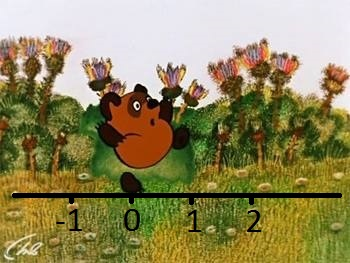
\includegraphics[width=80mm]{images/Winnie_the_Pooh_and_Medovuh.jpg}
    }
    \caption{Случайные бродилки.}
    \label{wun762hkej}
\end{figure}
\begin{enumerate}
  \item Сформулируйте центральную предельную теорему.
  \item При помощи центральной предельной теоремы оцените вероятность того, что ровно через час блужданий Винни-Пух окажется в области $(-\infty; \, -5]$.
  \item Используя неравенство Берри–Эссеена оцените погрешность вычислений предыдущего пункта.
\end{enumerate}


\item
Cлучайные величины $\xi$ и $\eta$ означают время безотказной работы рулевого управления и двигателя автомобиля соответственно. Время измеряется в годах. Совместная плотность имеет вид:
\[
f_{\xi, \,\eta}(x,\,y) =
\begin{cases}
0.005\,e^{-0.05\,x-0.1\,y} & \text{ при } x > 0, y > 0, \\
0                    & \text{ иначе.}
\end{cases}
\]

\begin{enumerate}
  \item Найдите частные плотности распределения случайных величин $\xi$ и $\eta$.
  \item Являются ли случайные величины $\xi$ и $\eta$ независимыми?
  \item Найдите вероятность того, что двигатель прослужит без сбоев более пяти лет.
  \item Найдите вероятность того, что двигатель прослужит без сбоев более восьми лет, если он уже проработал без сбоев три года.
  \item Найдите условное математическое ожидание безотказной работы рулевого управления, если двигатель проработал без сбоев пять лет,  $\E(\xi | \eta = 5)$.
  \item Найдите вероятность того, что рулевое управление проработает без сбоев на два года больше двигателя,  $\P(\{\xi - \eta > 2\})$.
\end{enumerate}

\item Бонусная задача

Случайная величина $\xi$ имеет плотность распределения
\[
    f_{\xi}(x) = \frac{1}{2} \cdot \frac{1}{\sqrt{2\pi}}e^{-\frac{(x-1)^2}{2}} + \frac{1}{2} \cdot \frac{1}{\sqrt{2\pi}}e^{-\frac{(x+1)^2}{2}} \text{.}
\]

\begin{enumerate}
\item Найдите $\E(\xi)$, $\E\left(\xi^2\right)$, $\Var(\xi)$.
\item Покажите, что функция $f_{\xi}(x)$, действительно, является плотностью распределения.
\end{enumerate}
\end{enumerate}


\newpage
\subsection[2015-2016]{\hyperref[sec:sol_kr_02_2015_2016]{2015-2016}}
\label{sec:kr_02_2015_2016}



\begin{enumerate}
\item Функция плотности случайного вектора $\xi=(\xi_1, \xi_2)^T$ имеет вид
\[
f(x,y)=\begin{cases}
0.5x + 1.5y, \text{ если } 0<x<1, \; 0<y<1 \\
0, \text{ иначе }
\end{cases}
\]
Найдите:
\begin{enumerate}
\item Математическое ожидание $\E(\xi_1 \cdot \xi_2)$
\item Условную плотность распределения $f_{\xi_1|\xi_2} (x|y)$
\item Условное математическое ожидание $\E(\xi_1| \xi_2=y)$
\item Константу $k$, такую, что функция $h(x,y)=kx\cdot f(x,y)$ будет являться совместной функцией плотности некоторой пары случайных величин
\end{enumerate}

\item На курсе учится очень много студентов. Вероятность того, что случайно выбранный студент по результатам рубежного контроля имеет хотя бы один незачет равна $0.2$. Пусть $\xi$ и $\eta$ — число студентов с незачетами и без незачетов в случайной группе из $10$ студентов. Найдите $\Cov(\xi,\eta)$, $\Corr(\xi,\eta)$, $\Cov(\xi-\eta,\xi)$. Являются ли случайные величины $\xi-\eta$ и $\xi$ независимыми?

\item Доходности акций компаний А и В – случайные величины $\xi$ и $\eta$. Известно, что $\E(\xi)=1$, $E(\eta)=1$, $\Var(\xi)=4$, $\Var(\eta)=9$, $\Corr(\xi,\eta)=-0.5$. Петя принимает решение потратить свой рубль на акции компании А, Вася — 50 копеек на акции компании А и 50 копеек на акции компании В, а Маша  принимает решение вложить свой рубль в портфель $R=\alpha\xi+(1-\alpha)\eta$, $(0 \leq \alpha \leq 1)$, обладающий минимальным риском. Найдите $\alpha$, ожидаемые доходности и риски портфелей Пети, Васи и Маши.

\item Будем считать, что рождение мальчика и девочки равновероятны.
\begin{enumerate}
\item Оцените с помощью неравенства Маркова вероятность того, что среди тысячи новорожденных младенцев, мальчиков будет более 75\%.
\item Оцените с помощью неравенства Чебышёва вероятность того, что доля мальчиков среди тысячи новорожденных младенцев будет отличаться от 0.5 более, чем на 0.25
\item С помощью теоремы Муавра-Лапласа вычислите вероятность из предыдущего пункта.
\end{enumerate}

\item Сейчас валютный курс племени «Мумба» составляет 100 оболов за один рубль. Изменение курса за один день — случайная величина $\delta_i$ с законом распределения:

\begin{center}
\begin{tabular}{lrrr}
\toprule
$x$ & $-1$ & $0$ & $2$ \\ \midrule
$\P(\delta_i = x)$ & $0.25$ & $0.5$ & $0.25$ \\
\bottomrule
\end{tabular}
\end{center}

Найдите вероятность того, что через полгода (171 день) рубль будет стоить более 250 оболов, если ежедневные изменения курса происходят независимо друг от друга.

\item \textbf{Бонусная задача}

Число посетителей, зашедших в магазин в течении дня — пуассоновская случайная величина с параметром $\lambda$. Каждый из посетителей совершает покупку с вероятностью $p$, не зависимо от других посетителей. Найдите математическое ожидание числа человек, совершивших покупку.

\end{enumerate}

% \section{Промежуточные экзамены}

% [1][3] 1 = one argument, 3 = value if missing
% эта магия создаёт окружение answerlist
% именно в окружении answerlist записаны варианты ответов в подключаемых exerciseXX
% просто \begin{answerlist} сделает ответы в три столбца
% если ответы длинные, то надо в них руками сделать
% \begin{answerlist}[1] чтобы они шли в один столбец
\newenvironment{answerlist}[1][3]{
\begin{multicols}{#1}
\begin{enumerate}[label=\fbox{\emph{\Alph*}},ref=\emph{\alph*}]
}
{
\end{enumerate}
\end{multicols}
}


\excludecomment{solution} % without solutions

\theoremstyle{definition}
\newtheorem{question}{Вопрос}


\subsection[2017-2018]{\hyperref[sec:sol_midterm_exam_2017_2018]{2017-2018}}
\label{sec:midterm_exam_2017_2018}



\begin{question}
Математическое ожидание величины \(X\) равно 2, а дисперсия равна 6.
Вероятность \(\P(X^2 \geq 100)\) лежит в диапазоне
\begin{answerlist}
  \item \([0;0.1]\)
  \item \([0.1;0.2]\)
  \item \([0.9;1]\)
  \item \([0.99;1]\)
  \item \([0;0.01]\)
\end{answerlist}
\end{question}

\begin{solution}
\begin{answerlist}
  \item Good answer :)
  \item Bad answer :(
  \item Bad answer :(
  \item Bad answer :(
  \item Bad answer :(
\end{answerlist}
\end{solution}



\begin{question}
Случайная величина \(\xi\) имеет распределение Пуассона с параметром
\(\lambda\). Математическое ожидание \(\E[\xi^2]\) равно
\begin{answerlist}
  \item \(\lambda\)
  \item \(e^{-\lambda}\)
  \item \(\lambda(1 - \lambda)\)
  \item \(\lambda^2\)
  \item \(\lambda(\lambda+1)\)
\end{answerlist}
\end{question}

\begin{solution}
\begin{answerlist}
  \item Bad answer :(
  \item Bad answer :(
  \item Bad answer :(
  \item Bad answer :(
  \item Good answer :)
\end{answerlist}
\end{solution}



\begin{question}
Известно, что \(\E(X)=-1\), \(\E(Y)=2\), \(\Var(X)=4\), \(\Var(Y)=9\),
\(\Cov(X,Y)=-3\). Корреляция \(\Corr(X+Y, Y)\) равна
\begin{answerlist}
  \item \(1/\sqrt{6}\)
  \item \(-1/\sqrt{7}\)
  \item \(2/\sqrt{7}\)
  \item \(-2/\sqrt{6}\)
  \item \(-3/\sqrt{6}\)
\end{answerlist}
\end{question}

\begin{solution}
\begin{answerlist}
  \item Bad answer :(
  \item Bad answer :(
  \item Good answer :)
  \item Bad answer :(
  \item Bad answer :(
\end{answerlist}
\end{solution}



\begin{question}
Совместное распределение дискретных случайных величин \(X\) и \(Y\)
задано таблицей:

\begin{tabular}{cccc}
\toprule
 & $Y=-2$ & $Y=0$ & $Y=1$ \\
\midrule
$X=3$ & $0.3$ & $0.1$ & $0.2$  \\
$X=6$ & $0.1$ & $0.2$ & $0.1$ \\
\bottomrule
\end{tabular}

Условное ожидание \(\E(X|Y=-2)\) равно
\begin{answerlist}
  \item \(3.75\)
  \item \(3.(3)\)
  \item \(3.25\)
  \item \(4.2\)
  \item \(3.5\)
\end{answerlist}
\end{question}

\begin{solution}
\begin{answerlist}
  \item Good answer :)
  \item Bad answer :(
  \item Bad answer :(
  \item Bad answer :(
  \item Bad answer :(
\end{answerlist}
\end{solution}



\begin{question}
Случайная величина \(\xi\) имеет стандартное нормальное распределение.
Вероятность \(\P(\{\xi \in [-1; \, 2]\})\) равна
\begin{answerlist}
  \item \(\int_{-1}^{2}\tfrac{1}{\sqrt{2\pi}}e^{x^2 / 2}\,dx\)
  \item \(\int_{-1}^{2}\tfrac{1}{\sqrt{2\pi}}e^{-x^2 / 2}\,dx\)
  \item \(\int_{-1}^{2}\tfrac{1}{\sqrt{2\pi}}e^{-x^2}\,dx\)
  \item \(\int_{-1}^{2}\tfrac{1}{2\pi}e^{-x^2 / 2}\,dx\)
  \item \(\int_{-1}^{2}\tfrac{1}{\sqrt{2\pi}}e^{x^2}\,dx\)
\end{answerlist}
\end{question}

\begin{solution}
\begin{answerlist}
  \item Bad answer :(
  \item Good answer :)
  \item Bad answer :(
  \item Bad answer :(
  \item Bad answer :(
\end{answerlist}
\end{solution}



\begin{question}
Для случайной величины \(X \sim \cN(\mu_X, \sigma^2_X)\) вероятность
\(\P(X - \mu_x > 5\sigma_X)\) примерно равна
\begin{answerlist}
  \item \(0\)
  \item \(0.5\)
  \item \(0.95\)
  \item \(1/5\)
  \item \(0.05\)
\end{answerlist}
\end{question}

\begin{solution}
\begin{answerlist}
  \item Good answer :)
  \item Bad answer :(
  \item Bad answer :(
  \item Bad answer :(
  \item Bad answer :(
\end{answerlist}
\end{solution}



\begin{question}
Двумерная случайная величина \((X, Y)\) равномерно распределена в
треугольнике ограниченном линиями \(x=0\), \(y=0\) и \(y+2x=4\).
Значение функции плотности \(f_{X,Y}(1,1)\) равно
\begin{answerlist}
  \item \(0.25\)
  \item \(0.5\)
  \item \(1\)
  \item \(\frac{1}{\sqrt{2\pi}}\exp(-0.5)\)
  \item \(0.125\)
\end{answerlist}
\end{question}

\begin{solution}
\begin{answerlist}
  \item Good answer :)
  \item Bad answer :(
  \item Bad answer :(
  \item Bad answer :(
  \item Bad answer :(
\end{answerlist}
\end{solution}



\begin{question}
У Васи есть пять кнопок, генерирующих целые числа от 1 до 6. Три
работают как честные кубики, одна — с увеличенной вероятностью
выпадения 6 (она выпадает с веростностью 0.5, остальные ---
равновероятно), одна — с увеличенной вероятностью выпадения 1 (она
выпадает с вероятностью 0.5, остальные — равновероятно). Вася нажимает
на случайную кнопку. Число 6 выпадет с вероятностью
\begin{answerlist}
  \item 0.11
  \item 0.12
  \item 1/4
  \item 1/6
  \item 0.22
\end{answerlist}
\end{question}

\begin{solution}
\begin{answerlist}
  \item Bad answer :(
  \item Bad answer :(
  \item Bad answer :(
  \item Bad answer :(
  \item Good answer :)
\end{answerlist}
\end{solution}



\begin{question}
Величины \(X_1\), \(X_2\), \ldots, независимы и одинаково распределены с
\(\E(X_i) = 4\) и \(\Var(X_i) = 100\), а
\(S_n = X_1 + X_2 + \ldots + X_n\). К нормальному стандартному
распределению сходится последовательность
\begin{answerlist}
  \item \(\sqrt{n}\frac{S_n - 4n}{10/\sqrt{n}}\)
  \item \(\sqrt{n}\frac{S_n - 4}{10}\sqrt{n}\)
  \item \(\sqrt{n}\frac{S_n - 4}{10}\)
  \item \(\frac{S_n - 4n}{10\sqrt{n}}\)
  \item \(\sqrt{n}\frac{S_n - 4}{10/\sqrt{n}}\)
\end{answerlist}
\end{question}

\begin{solution}
\begin{answerlist}
  \item Bad answer :(
  \item Bad answer :(
  \item Bad answer :(
  \item Good answer :)
  \item Bad answer :(
\end{answerlist}
\end{solution}



\begin{question}
События A, B и C независимы в совокупности, если
\begin{answerlist}
  \item \(\P(A|B) = \P(A), \P(A|C) = \P(A)\)
  \item \(\P(ABC) = \P(A) \P(B) \P(C)\)
  \item \(\P(A|B) = \P(A), \P(A|C) = \P(A), \P(B|C) = \P(B)\)
  \item \(\P(A\cap B) = \P(A)\P(B), \P(A\cap C) = \P(A)\P(C), \P(B\cap C) = \P(B)\P(C)\)
  \item \(\P(A \cap B \cap C) = 0\)
\end{answerlist}
\end{question}

\begin{solution}
\begin{answerlist}
  \item Bad answer :(
  \item Bad answer :(
  \item Bad answer :(
  \item Bad answer :(
  \item Bad answer :(
\end{answerlist}
\end{solution}



\begin{question}
Случайная величина \(\xi\) имеет равномерное распределение на отрезке
\([0;\,4]\). Вероятность \(\P(\{\xi \in [3;\,6]\})\) равна
\begin{answerlist}
  \item \(\Phi(4) - \Phi(3)\)
  \item \(1/4\)
  \item \(3/6\)
  \item \(1/2\)
  \item \(3/4\)
\end{answerlist}
\end{question}

\begin{solution}
\begin{answerlist}
  \item Bad answer :(
  \item Good answer :)
  \item Bad answer :(
  \item Bad answer :(
  \item Bad answer :(
\end{answerlist}
\end{solution}



\begin{question}
Случайная величина \(X\) принимает равновероятно целые значение от
\(-5\) до \(5\) включительно. Случайная величина \(Y\) принимает
равновероятно целые значение от \(-1\) до \(1\) включительно. Величины
\(X\) и \(Y\) независимы. Вероятность \(\P(X+Y^2=2)\) равна
\begin{answerlist}
  \item \(1/5\)
  \item \(1/33\)
  \item \(1/11\)
  \item \(5/33\)
  \item \(2/33\)
\end{answerlist}
\end{question}

\begin{solution}
\begin{answerlist}
  \item Bad answer :(
  \item Bad answer :(
  \item Good answer :)
  \item Bad answer :(
  \item Bad answer :(
\end{answerlist}
\end{solution}



\begin{question}
Известно, что \(\E(X)=-1\), \(\E(Y)=2\), \(\Var(X)=4\), \(\Var(Y)=9\),
\(\Cov(X,Y)=-3\). Ковариация \(\Cov(aX, (1-a)Y)\) минимальна при \(a\)
равном
\begin{answerlist}
  \item \(3/12\)
  \item \(0\)
  \item \(1/2\)
  \item \(-1/4\)
  \item \(2/3\)
\end{answerlist}
\end{question}

\begin{solution}
\begin{answerlist}
  \item Bad answer :(
  \item Bad answer :(
  \item Good answer :)
  \item Bad answer :(
  \item Bad answer :(
\end{answerlist}
\end{solution}



\begin{question}
Круг разделён на секторы с углом \(\frac{\pi}{3}\). Один из них закрашен
красным, один сектор --- синим, остальные сектора --- белым. Вася кидает
дротики и всегда попадает в круг, все точки круга равновероятны.
Вероятность того, что Вася попадёт в красный сектор, равна
\begin{answerlist}
  \item не хватает данных
  \item 1/4
  \item \(\pi / 3\)
  \item \(\pi / 6\)
  \item 1/6
\end{answerlist}
\end{question}

\begin{solution}
\begin{answerlist}
  \item Bad answer :(
  \item Bad answer :(
  \item Bad answer :(
  \item Bad answer :(
  \item Good answer :)
\end{answerlist}
\end{solution}



\begin{question}
Двумерная функция распределения \(F_{X,Y}(x,y)\) может \textbf{НЕ}
удовлетворять свойству
\begin{answerlist}
  \item функция \(F_{X,Y}(x, y)\) непрерывна
  \item \(\lim_{y \to +\infty} F_{X,Y}(x,y) = F_X(x)\)
  \item \(F_{X,Y}(x,y)\) не убывает по \(x\)
  \item \(0 \leq F_{X,Y}(x, y)\leq 1\)
  \item \(\lim_{x,y \to +\infty} F_{X,Y}(x,y) = 1\)
\end{answerlist}
\end{question}

\begin{solution}
\begin{answerlist}
  \item Bad answer :(
  \item Bad answer :(
  \item Good answer :)
  \item Bad answer :(
  \item Bad answer :(
\end{answerlist}
\end{solution}



\begin{question}
Известно, что \(\P(A \cap B) = 0.2\), \(\P(A \cup B) = 0.6\),
\(\P(A) = 0.3\). Вероятность \(\P(B)\) равна
\begin{answerlist}
  \item 0.3
  \item 0.5
  \item 0.1
  \item не хватает данных
  \item 0.6
\end{answerlist}
\end{question}

\begin{solution}
\begin{answerlist}
  \item Bad answer :(
  \item Good answer :)
  \item Bad answer :(
  \item Bad answer :(
  \item Bad answer :(
\end{answerlist}
\end{solution}



\begin{question}
Известно, что \(\E(X)=-1\), \(\E(Y)=2\), \(\Var(X)=4\), \(\Var(Y)=9\),
\(\Cov(X,Y)=-3\). Дисперсия \(\Var(2X-Y+1)\) равна
\begin{answerlist}
  \item 31
  \item \(37\)
  \item \(24\)
  \item \(-31\)
  \item 34
\end{answerlist}
\end{question}

\begin{solution}
\begin{answerlist}
  \item Bad answer :(
  \item Good answer :)
  \item Bad answer :(
  \item Bad answer :(
  \item Bad answer :(
\end{answerlist}
\end{solution}



\begin{question}
Величины \(X_1\), \(X_2\), \ldots, независимы и одинаково распределены
\(\cN(0;1)\). Предел по вероятности
\(\plim_{n\to\infty} \frac{X_1^2+ X_2^2 + \ldots + X_n^2}{n}\) равен
\begin{answerlist}
  \item \(3\)
  \item \(1\)
  \item \(2\)
  \item \(0\)
  \item \(1/2\)
\end{answerlist}
\end{question}

\begin{solution}
\begin{answerlist}
  \item Bad answer :(
  \item Good answer :)
  \item Bad answer :(
  \item Bad answer :(
  \item Bad answer :(
\end{answerlist}
\end{solution}



\begin{question}
Совместная функция плотности величин \(X\) и \(Y\) имеет вид \[
f(x,y) =
\begin{cases}
6xy^2, \text{ при } x, y \in [0;1] \\
0, \text{ иначе } \\
\end{cases}.
\] При \(Y=1/2\) величина \(X\) имеет условное распределение
\begin{answerlist}
  \item с плотностью \(f(x)=1.5x\) при \(x\in[0;1]\)
  \item равномерное, \(U[0;1]\)
  \item с плотностью \(f(x)=2x\) при \(x\in[0;1]\)
  \item нормальное, \(\cN(0;1)\)
  \item с плотностью \(f(x)=3x^2\) при \(x\in[0;1]\)
\end{answerlist}
\end{question}

\begin{solution}
\begin{answerlist}
  \item Bad answer :(
  \item Bad answer :(
  \item Good answer :)
  \item Bad answer :(
  \item Bad answer :(
\end{answerlist}
\end{solution}



\begin{question}
Известно, что \(\E(X)=-1\), \(\E(Y)=2\), \(\Var(X)=4\), \(\Var(Y)=9\),
\(\Cov(X,Y)=-3\). Ожидание \(\E(X^2-Y^2)\) равно
\begin{answerlist}
  \item \(-4\)
  \item 8
  \item 4
  \item \(-8\)
  \item 0
\end{answerlist}
\end{question}

\begin{solution}
\begin{answerlist}
  \item Bad answer :(
  \item Bad answer :(
  \item Bad answer :(
  \item Good answer :)
  \item Bad answer :(
\end{answerlist}
\end{solution}



\begin{question}
Величины \(X_1\), \(X_2\), \ldots, независимы и одинаково распределены с
\(\E(X_i) = 4\) и \(\Var(X_i) = 100\). Вероятность
\(\P(\bar X_n \leq 5)\) примерно равна
\begin{answerlist}
  \item \(0.50\)
  \item \(0.28\)
  \item \(0.84\)
  \item \(0.95\)
  \item \(0.67\)
\end{answerlist}
\end{question}

\begin{solution}
\begin{answerlist}
  \item Bad answer :(
  \item Bad answer :(
  \item Good answer :)
  \item Bad answer :(
  \item Bad answer :(
\end{answerlist}
\end{solution}



\begin{question}
Известно, что \(\E(X)=-1\), \(\E(Y)=2\), \(\Var(X)=4\), \(\Var(Y)=9\),
\(\Cov(X,Y)=-3\). Ковариация \(\Cov(X+2Y, 2X+3)\) равна
\begin{answerlist}
  \item \(-4\)
  \item \(1\)
  \item \(4\)
  \item \(0\)
  \item \(-1\)
\end{answerlist}
\end{question}

\begin{solution}
\begin{answerlist}
  \item Good answer :)
  \item Bad answer :(
  \item Bad answer :(
  \item Bad answer :(
  \item Bad answer :(
\end{answerlist}
\end{solution}



\begin{question}
Известно, что \(\E(X)=-1\), \(\E(Y)=2\), \(\Var(X)=4\), \(\Var(Y)=9\),
\(\Cov(X,Y)=-3\). Ожидание \(\E((X-1)Y)\) равно
\begin{answerlist}
  \item \(-6\)
  \item \(-7\)
  \item \(-5\)
  \item \(-8\)
  \item \(-9\)
\end{answerlist}
\end{question}

\begin{solution}
\begin{answerlist}
  \item Bad answer :(
  \item Good answer :)
  \item Bad answer :(
  \item Bad answer :(
  \item Bad answer :(
\end{answerlist}
\end{solution}



\begin{question}
В каком из этих случаев события \(A\) и \(B\) будут независимы?
\begin{answerlist}
  \item \(\P(A \cup B) = 0.6\), \(\P (A) = 0.5\), \(\P(B) = 0.2\)
  \item \(\P(A \cap B) = 0.1\), \(\P (A) = 0.5\), \(\P(B) = 0.2\)
  \item \(\P(A \cap B) = 0\), \(\P (A) = 0.8\), \(\P(B) = 0.1\)
  \item \(\P(A \cup B) = 0.2\), \(\P (A) = 0.5\), \(\P(B) = 0.4\)
  \item \(\P(A \cap B) = 0.1\), \(\P (A) = 0.5\), \(\P(B) = 0.9\)
\end{answerlist}
\end{question}

\begin{solution}
\begin{answerlist}
  \item Bad answer :(
  \item Good answer :)
  \item Bad answer :(
  \item Bad answer :(
  \item Bad answer :(
\end{answerlist}
\end{solution}



\begin{question}
Правильный кубик подбрасывается два раза, величина \(X_i\) равна 1, если
в \(i\)-ый раз выпала шестёрка, и нулю иначе. Условный закон
распределения \(X_1\) при условии \(X_1+X_2=1\) совпадает с
распределением
\begin{answerlist}
  \item Биномиальным \(Bin(n=2, p=1/2)\)
  \item Бернулли с \(p=1/2\)
  \item Бернулли с \(p=1/6\)
  \item Биномиальным \(Bin(n=2, p=1/6)\)
  \item нормальным \(\cN(0;1)\)
\end{answerlist}
\end{question}

\begin{solution}
\begin{answerlist}
  \item Bad answer :(
  \item Good answer :)
  \item Bad answer :(
  \item Bad answer :(
  \item Bad answer :(
\end{answerlist}
\end{solution}



\begin{question}
Случайные величины \(X\) и \(Y\) независимы и нормально распределены с
параметрами \(\E(X)=2\), \(\Var(X)=3\), \(\E(Y)=1\), \(\Var(Y)=4\).
Вероятность \(\P(X+Y<3)\) равна
\begin{answerlist}
  \item \(3/7\)
  \item \(0.05\)
  \item \(0.5\)
  \item \(0.995\)
  \item \(2/7\)
\end{answerlist}
\end{question}

\begin{solution}
\begin{answerlist}
  \item Bad answer :(
  \item Bad answer :(
  \item Good answer :)
  \item Bad answer :(
  \item Bad answer :(
\end{answerlist}
\end{solution}



\begin{question}
У Васи есть пять кнопок, генерирующих целые числа от 1 до 6. Три
работают как честные кубики, одна — с увеличенной вероятностью
выпадения 6 (она выпадает с веростностью 0.5, остальные ---
равновероятно), одна — с увеличенной вероятностью выпадения 1 (она
выпадает с вероятностью 0.5, остальные — равновероятно). Вася нажимает
на случайную кнопку. После нажатия на случайную кнопку выпала 6.
Условная вероятность того, что это была кнопка «честный кубик» равна
\begin{answerlist}
  \item 1/2
  \item 4/11
  \item 5/11
  \item 8/11
  \item 6/11
\end{answerlist}
\end{question}

\begin{solution}
\begin{answerlist}
  \item Bad answer :(
  \item Bad answer :(
  \item Good answer :)
  \item Bad answer :(
  \item Bad answer :(
\end{answerlist}
\end{solution}



\begin{question}
Ковариационной матрицей может являться матрица
\begin{answerlist}
  \item \(\begin{pmatrix} 1 & 2 \\ 2 & 1 \\ \end{pmatrix}\)
  \item \(\begin{pmatrix} 1 & 4 \\ 4 & 9 \\ \end{pmatrix}\)
  \item \(\begin{pmatrix} 9 & 7 \\ 7 & 6 \\ \end{pmatrix}\)
  \item \(\begin{pmatrix} -1 & 2 \\ 2 & 10 \\ \end{pmatrix}\)
  \item \(\begin{pmatrix} 1 & 2 \\ 1 & 2 \\ \end{pmatrix}\)
\end{answerlist}
\end{question}

\begin{solution}
\begin{answerlist}
  \item Bad answer :(
  \item Bad answer :(
  \item Good answer :)
  \item Bad answer :(
  \item Bad answer :(
\end{answerlist}
\end{solution}



\begin{question}
Известно, что \(\E(X)=-1\), \(\E(Y)=2\), \(\Var(X)=4\), \(\Var(Y)=9\),
\(\Cov(X,Y)=-3\). Из условия \(\E(aX+(1-a)Y)=0\) следует, что \(a\)
равно
\begin{answerlist}
  \item 2/3
  \item 1/2
  \item 1
  \item 0
  \item 1/3
\end{answerlist}
\end{question}

\begin{solution}
\begin{answerlist}
  \item Good answer :)
  \item Bad answer :(
  \item Bad answer :(
  \item Bad answer :(
  \item Bad answer :(
\end{answerlist}
\end{solution}



\begin{question}
Случайная величина \(\xi\) имеет биномиальное распределение с
параметрами \(n = 2\) и \(p = 3/4\). Вероятность \(\P(\xi = 0)\) равна
\begin{answerlist}
  \item \(1/2\)
  \item \(1/16\)
  \item \(9/16\)
  \item \(3/4\)
  \item \(3/4\)
\end{answerlist}
\end{question}

\begin{solution}
\begin{answerlist}
  \item Bad answer :(
  \item Good answer :)
  \item Bad answer :(
  \item Bad answer :(
  \item Bad answer :(
\end{answerlist}
\end{solution}



\begin{question}
Количество сбоев системы SkyNet за сутки имеет распределение Пуассона.
Среднее количество сбоев за сутки равно 4. Вероятность того, что за
сутки произойдет не менее одного сбоя, равна
\begin{answerlist}
  \item \(e^4\)
  \item \(1-e^4\)
  \item \(1- e^{-4}\)
  \item \(\tfrac{1}{4!}e^{-4}\)
  \item \(e^{-4}\)
\end{answerlist}
\end{question}

\begin{solution}
\begin{answerlist}
  \item Bad answer :(
  \item Bad answer :(
  \item Good answer :)
  \item Bad answer :(
  \item Bad answer :(
\end{answerlist}
\end{solution}



\begin{question}
У пары случайных величин \(X\), \(Y\) существует совместная функция
плотности \(f(x,y)\) и условная функция плотности \(f(x|y)\). Условную
дисперсию \(\Var(X|Y)\) можно найти по формуле
\begin{answerlist}
  \item \(\int_{-\infty}^{+\infty} (x - \E(X|Y))^2 \, dx\)
  \item \(\int_{-\infty}^{+\infty} (x - \E(X))^2 f(x|Y) \, dx\)
  \item \(\int_{-\infty}^{+\infty} x^2 f(x|Y) \, dx - (\E(X|Y))^2\)
  \item \(\left(\int_{-\infty}^{+\infty} x f(x|Y) \, dx\right)^2 - (\E(X|Y))^2\)
  \item \(\int_{-\infty}^{+\infty} x^2 f(x|Y) \, dx\)
\end{answerlist}
\end{question}

\begin{solution}
\begin{answerlist}
  \item Bad answer :(
  \item Bad answer :(
  \item Good answer :)
  \item Bad answer :(
  \item Bad answer :(
\end{answerlist}
\end{solution}



\begin{question}
Случайная величина \(\xi\) имеет распределение Бернулли с параметром
\(p\). Математическое ожидание \(\E[\xi^2]\) равно
\begin{answerlist}
  \item \(p(1-p)\)
  \item \(p\)
  \item \(p^2\)
  \item \(0\)
  \item \(1-p\)
\end{answerlist}
\end{question}

\begin{solution}
\begin{answerlist}
  \item Bad answer :(
  \item Good answer :)
  \item Bad answer :(
  \item Bad answer :(
  \item Bad answer :(
\end{answerlist}
\end{solution}



\begin{question}
Случайная величина \(\xi\) имеет показательное (экспоненциальное)
распределение с параметром \(\lambda\). Математическое ожидание
\(\E[\xi^2]\) равно
\begin{answerlist}
  \item \(2/\lambda^2\)
  \item \(1/\lambda^2 - 1/ \lambda\)
  \item \(\lambda^2\)
  \item \(1/\lambda\)
  \item \(1/\lambda^2\)
\end{answerlist}
\end{question}

\begin{solution}
\begin{answerlist}
  \item Good answer :)
  \item Bad answer :(
  \item Bad answer :(
  \item Bad answer :(
  \item Bad answer :(
\end{answerlist}
\end{solution}



\begin{question}
Круг разделён на секторы с углом \(\frac{\pi}{3}\). Один из них закрашен
красным, один --- синим, остальные --- белым. Вася кидает дротики и
всегда попадает в круг, все точки круга равновероятны. Пусть событие
\(A\) --- попадание в красный сектор, \(B\) --- попадание в синий
сектор. Эти события
\begin{answerlist}
  \item образуют полную группу событий
  \item случаются с вероятностями 1/4
  \item независимы
  \item случаются с разными вероятностями
  \item несовместны
\end{answerlist}
\end{question}

\begin{solution}
\begin{answerlist}
  \item Bad answer :(
  \item Bad answer :(
  \item Bad answer :(
  \item Bad answer :(
  \item Good answer :)
\end{answerlist}
\end{solution}



\begin{question}
Совместная функция плотности величин \(X\) и \(Y\) имеет вид \[
f(x,y) =
\begin{cases}
6xy^2, \text{ при } x, y \in [0;1] \\
0, \text{ иначе } \\
\end{cases}.
\]

Математическое ожидание \(\E(XY)\) равно
\begin{answerlist}
  \item \(1/2\)
  \item \(1\)
  \item \(4/5\)
  \item \(3/4\)
  \item \(2/3\)
\end{answerlist}
\end{question}

\begin{solution}
\begin{answerlist}
  \item Good answer :)
  \item Bad answer :(
  \item Bad answer :(
  \item Bad answer :(
  \item Bad answer :(
\end{answerlist}
\end{solution}



\begin{question}
Случайная величина \(\xi\) имеет равномерное распределение на отрезке
\([0;\,4]\). Математическое ожидание \(\E[\xi^2]\) равно
\begin{answerlist}
  \item \(52/12\)
  \item \(2\)
  \item \(4\)
  \item \(16/12\)
  \item \(64/12\)
\end{answerlist}
\end{question}

\begin{solution}
\begin{answerlist}
  \item Bad answer :(
  \item Bad answer :(
  \item Bad answer :(
  \item Bad answer :(
  \item Good answer :)
\end{answerlist}
\end{solution}



\begin{question}
Известно, что \(\E(X)=-1\), \(\E(Y)=2\), \(\Var(X)=4\), \(\Var(Y)=9\),
\(\Cov(X,Y)=-3\). Дисперсия \(\Var(aX+(1-a)Y)\) минимальна при \(a\)
равном
\begin{answerlist}
  \item 11/12
  \item 7/12
  \item \(3/12\)
  \item \(-1/4\)
  \item 3/24
\end{answerlist}
\end{question}

\begin{solution}
\begin{answerlist}
  \item Good answer :)
  \item Bad answer :(
  \item Bad answer :(
  \item Bad answer :(
  \item Bad answer :(
\end{answerlist}
\end{solution}



\begin{question}
В самолёте 200 пассажиров. Четверть пассажиров летит без багажа,
половина из них --- с рюкзаками. Среди пассажиров с багажом 55 человек
летит с рюкзаками. Вероятность того, что случайно выбранный человек
летит без рюкзака, равна
\begin{answerlist}
  \item 0.6
  \item 0.4
  \item 0.65
  \item 0.45
  \item 0.5
\end{answerlist}
\end{question}

\begin{solution}
\begin{answerlist}
  \item Good answer :)
  \item Bad answer :(
  \item Bad answer :(
  \item Bad answer :(
  \item Bad answer :(
\end{answerlist}
\end{solution}



\begin{question}
Математическое ожидание величины \(X\) равно 2, а дисперсия равна 6.
Вероятность \(\P(|2-X|\leq 10)\) принадлежит диапазону
\begin{answerlist}
  \item \([0.2;0.4]\)
  \item \([0; 0.06]\)
  \item \([0.94; 1]\)
  \item \([0.6; 0.8]\)
  \item \([0.99;1]\)
\end{answerlist}
\end{question}

\begin{solution}
\begin{answerlist}
  \item Bad answer :(
  \item Bad answer :(
  \item Good answer :)
  \item Bad answer :(
  \item Bad answer :(
\end{answerlist}
\end{solution}



\newpage
\thispagestyle{empty}
\section{Контрольная работа 3}


\subsection[2017-2018]{\hyperref[sec:sol_kr_03_2017_2018]{2017-2018}}
\label{sec:kr_03_2017_2018}

\subsubsection*{Минимум}

\begin{enumerate}
\item Дайте определение выборочной функции распределения.
\item Предположим, что величины $X_1$, $X_2$, \ldots, $X_n$ независимы и нормальны
$\cN(\mu;\sigma^2)$. Укажите закон распределения выборочного среднего, величины
$\frac{\bar X - \mu}{\sigma/\sqrt{n}}$, величины $\frac{\bar X - \mu}{\hat\sigma/\sqrt{n}}$,
величины $\frac{\hat\sigma^2(n-1)}{\sigma^2}$.
\item Рост в сантиметрах, случайная величина $X$, и вес в килограммах, случайная
величина $Y$, взрослого мужчины является нормальным случайным вектором $Z = (X, Y)$
с математическим ожиданием $\E(Z) = (175, 75)$ и ковариационной матрицей

\[
\Var(Z) =
\begin{pmatrix}
49 & 28 \\
28 & 36
\end{pmatrix}
\]

\begin{enumerate}
\item Найдите средний вес мужчины при условии, что его рост составляет $172$ см.
\item Выпишите условную плотность распределения веса мужчины при условии, что его
рост составляет $172$ см.
\item Найдите условную вероятность того, что человек будет иметь вес, больший $92$ кг,
при условии, что его рост составляет $172$ см.
\end{enumerate}

\item Стоимость выборочного исследования генеральной совокупности, состоящей из трёх
страт, определяется по формуле $TC = c_1n_1 + c_2n_2 + c_3n_3$, где $c_i$ — цена
одного наблюдения в $i$-ой страте, a $n_i$ — число наблюдений, которые приходятся
на $i$-ую страту. Найдите $n_1$, $n_2$ и $n_3$, при которых дисперсия стратифицированного
среднего достигает наименьшего значения, если бюджет исследования 8000 и имеется
следующая информация:

\begin{center}
\begin{tabular}{cccc}
\toprule
Страта & $1$ & $2$ & $3$  \\
\midrule
Среднее значение & $30$ & $40$ & $50$ \\
Стандартная ошибка  & $5$ & $10$ & $20$ \\
Вес & $25\%$ & $25\%$ & $50\%$ \\
Цена наблюдения & $2$ & $5$ & $8$ \\
\bottomrule
\end{tabular}
\end{center}
\end{enumerate}


\subsubsection*{Задачи}

\begin{enumerate}[resume]
	%Задача 1
\item Пусть $X_{1}, \ldots, X_{n}$ выборка из нормального распределения $N(\mu,1)$.
\begin{enumerate}
\item Выпишите функцию правдоподобия;
\item Методом максимального правдоподобия найдите оценку $\hat{\mu}$ математического
ожидания $\mu$;
\item Проверьте состоятельность и несмещённость оценки $\hat{\mu}$;
\item Вычислите информацию Фишера о параметре $\mu$, содержащуюся во всей выборке;
\item Для произвольной несмещённой оценки $\mu$ выпишите неравенство Рао-Крамера-Фреше;
\item Проверьте свойство эффективности оценки $\hat{\mu}$;
\item Найдите оценку максимального правдоподобия $\hat{\theta}$ для второго начального
момента;
\item Проверьте свойства несмещенности и асимптотической несмещенности оценки $\hat{\theta}$;
\item С помощью дельта-метода вычислите, примерно, дисперсию оценки $\hat{\theta}$;
\item Проверьте состоятельность оценки $\hat{\theta}$.
\end{enumerate}

 %Задача 2
 \item Пусть $X_{1}$, \ldots, $X_{n}$ выборка из распределения с функцией плотности:

\[
f(x)=\begin{cases}
\frac{2}{\theta^2}(\theta-x),&\text{при }x\in[0,\theta]\\
0,&\text{при }x\notin[0,\theta]
\end{cases}
\]

\begin{enumerate}
\item Методом моментов найдите оценку параметра $\theta$;
\item Приведите определение состоятельности оценки и проверьте, будет ли найденная
оценка состоятельной.
\end{enumerate}

%Задача 3
\item В прихожей лежат четыре карты «тройка». На двух из них нет денег, на двух
других 30 и 500 рублей. Вовочка не помнит, на какой из карт есть деньги, поэтому
берёт три карточки.

\begin{enumerate}
\item Найдите математическое ожидание и дисперсию средней по выбранным карточкам
суммы денег;
\item Определите, какова вероятность того, что Вовочке удастся войти в метро,
если стоимость проезда по тройке составляет 35 рублей.
\end{enumerate}

	%Задача 4
\item По выборочному опросу студенческих семейных пар о расходах на ланч были
получены следующие результаты:

\begin{center}
\begin{tabular}{ccccc}
\toprule
Номер семьи & 1 & 2 & 3 & 4\\
Расходы мужа & 450 & 370 & 170 & 200\\
Расходы жены & 210 & 350 & 250 & 180\\
\bottomrule
\end{tabular}
\end{center}

Считая, что разница в расходах мужа и жены хорошо описываются нормальным распределением,
постройте 95\%-ый доверительный интервал для разницы математических ожиданий расходов
супругов. Есть ли основания утверждать, что расходы одинаковы?

	%Задание №5
\item Наблюдатель Алексей Недопускальный решил проверить честность выборов.
Ему удалось подглядеть, как проголосовали 60 избирателей. Из них 42 выбрали
действующего президента.

\begin{enumerate}
\item Постройте 95\%-ый доверительный интервал для истинной доли избирателей,
проголосовавших «за» действующего президента.
\item По результатам ЦентрИзберКома «за» действующего президента проголосовало
76.67\% населения. Согласуются ли эти данные с данными Алексея?
\item Сколько бюллетеней нужно подглядеть Алексею, чтобы с вероятностью
$0.95$ отклонение от выборочной доли проголосовавших «за» действующего
президента от истинной не превышало $0.01$?
\end{enumerate}
\end{enumerate}



\newpage
\subsection[2016-2017]{\hyperref[sec:sol_kr_03_2016_2017]{2016-2017}}
\label{sec:kr_03_2016_2017}

\begin{enumerate}

\item Дана реализация случайной выборки: $1$, $10$, $7$, $4$, $-2$. Выпишите
определения и найдите значения следующих характеристик:
\begin{enumerate}
  \item вариационного ряда,
  \item выборочного среднего,
  \item выборочной дисперсии,
  \item несмещенной оценки дисперсии,
  \item выборочного второго начального момента.
  \item Постройте выборочную функцию распределения.
\end{enumerate}


\item
Мама дяди Фёдора каждое лето приезжает в Простоквашино с тремя вечерними платьями.
Если выбирать одно платье из трёх случайно, то ожидание стоимости равно 11 тысяч рублей,
а дисперсия стоимости равна 3 тысячи квадратных рублей.
Рачительный кот Матроскин случайным образом выбирает одно из платьев и продаёт его как ненужное. Вычислите математическое ожидание и дисперсию стоимости двух оставшихся платьев.

\item
Ресторанный критик ходит по трём типам ресторанов (дешевых, бюджетных и дорогих)
города N для того, чтобы оценить среднюю стоимость бизнес-ланча. В городе 40\%
дешевых ресторанов, 50\% — бюджетных и 10\% — дорогих. Стандартное отклонение
цены бизнес-ланча составляет 10, 30 и 60 рублей соответственно. В ресторане
критик заказывает только кофе. Стоимость кофе в дешевых/бюджетных/дорогих ресторанах
составляет 150, 300 и 600 рублей соответственно, а бюджет исследования — 30\,000 рублей.
\begin{enumerate}
  \item Какое количество ресторанов каждого типа нужно посетить критику, чтобы
	как можно точнее оценить среднюю стоимость бизнес-ланча при заданном бюджетном
	ограничении (округлите полученные значения до ближайших целых)?
  \item Вычислите дисперсию соответствующего стратифицированного среднего.
\end{enumerate}

\item
В «акции протеста против коррупции» в Москве 26.03.2017 по данным МВД приняло
участие 8\,000 человек. Считая, что население Москвы составляет 12\,300\,000 человек,
постройте 95\% доверительный интервал для истинной доли желающих участвовать в
подобных акциях жителей России. Можно ли утверждать, что эта доля статистически
не отличается от нуля?

\item
Для некоторой отрасли проведено исследование об оплате труда мужчин и женщин. Их зарплаты (тыс. руб. в месяц) приведены ниже:
\begin{center}
\begin{tabular}{cccccc}
  \toprule
  \text{мужчины}         &$50$    &$40$    &$45$   &$45$   &$35$   \\
  \text{женщины}         &$60$    &$30$    &$30$   &$35$   &$30$   \\ \bottomrule
\end{tabular}
\end{center}

\begin{enumerate}
  \item Считая, что распределение заработных плат мужчин хорошо описывается
	нормальным распределением, постройте
  \begin{enumerate}
    \item 99\%-ый доверительный интервал для математического ожидания заработной
		платы мужчин,
    \item 90\%-ый доверительный интервал для стандартного отклонения заработной
		платы мужчин.
  \end{enumerate}
  \item
  \begin{enumerate}
    \item Сформулируйте предпосылки, необходимые для построения доверительно интервала
		для разности математических ожиданий заработных плат мужчин и женщин.
    \item Считая предпосылки выполненными, постройте 90\%-ый доверительный интервал
		для разности математических ожиданий заработных плат мужчин и женщин.
    \item Можно ли считать зарплаты мужчин и женщин одинаковыми?
  \end{enumerate}
\end{enumerate}

\item
Пусть $X = (X_1, \, \ldots, \, X_n)$ — случайная выборка из нормального распределения
с нулевым математическим ожиданием и дисперсией $\theta$.
\begin{enumerate}
  \item Используя второй начальный момент, найдите оценку параметра $\theta$
	методом моментов.
  \item Сформулируйте определение несмещённости оценки и проверьте выполнение
	данного свойства для оценки, найденной в пункте а).
  \item Сформулируйте определение состоятельности оценки и проверьте выполнение
	данного свойства для оценки, найденной в пункте а).
  \item Найдите оценку параметра $\theta$ методом максимального правдоподобия.
  \item Вычислите информацию Фишера о параметре $\theta$, заключенную в $n$
	наблюдениях случайной выборки.
  \item Сформулируйте неравенство Рао-Крамера-Фреше.
  \item Сформулируйте определение эффективности оценки и проверьте выполнение
	данного свойства для оценки, найденной в пункте г).
\end{enumerate}

\item
Аэрофлот утверждает, что 10\% пассажиров, купивших билет, не являются на рейс.
В случайной выборке из шести рейсов аэробуса А320, имеющего 180 посадочных мест,
число не явившихся оказалось: $5$, $10$, $25$, $0$, $17$, $30$. Пусть число пассажиров
$X$, не явившихся на рейс, хорошо описывается распределением Пуассона $\P(X = k)
= \tfrac{\lambda^{k}}{k!}e^{-\lambda}$, $k \in \{0,\, 1,\, 2,\, \ldots\}$. При
помощи метода максимального правдоподобия найдите:
\begin{enumerate}
  \item оценку $\E(X)$ и её числовое значение по выборке,
  \item оценку дисперсии $X$ и её числовое значение по выборке,
  \item оценку стандартного отклонения $X$ и её числовое значение по выборке,
  \item оценку вероятности того, что на рейс явятся все пассажиры, а также найдите
	её числовое значение по выборке.
  \item Используя асимптотические свойства оценок максимального правдоподобия,
	постройте 95\% доверительный интервал для $\E(X)$.
  \item С помощью дельта-метода найдите 95\% доверительный интервал для вероятности
	полной загруженности самолёта.
\end{enumerate}
\end{enumerate}


\newpage
\subsection[2015-2016]{\hyperref[sec:sol_kr_03_2015_2016]{2015-2016}}
\label{sec:kr_03_2015_2016}

\epigraph{Ищите и обрящете, толцыте и отверзется вам}{Лука 11:9}

\begin{enumerate}
\item В студенческом буфете осталось только три булочки одинаковой привлекательности
и цены, но разной калорийности: 250, 400 и 550 ккал. Голодные Маша и Саша, не глядя
на калорийность, покупают по булочке. Найдите математическое ожидание и дисперсию
суммы поглощенных студентами калорий.
\item Дана реализация случайной выборки  независимых одинаково распределенных
случайных величин: 11, 4, 6.
\begin{enumerate}
  \item Выпишите вариационный ряд;
  \item Постройте выборочную функцию распределения;
  \item Найдите выборочную медиану распределения;
  \item Вычислите выборочное среднее и несмещенную оценку дисперсии.
\end{enumerate}

\item Найдите математическое ожидание, дисперсию и коэффициент корреляции случайных
величин $X$ и $Y$, совместное распределение которых имеет функцию плотности
\[
f(x, y) = \frac{5}{4\pi \sqrt{6}} \exp\left(
-\frac{25}{48}\left( (x-1)^2 -0.4(x-1)y + y^2 \right)
\right)
\]

\item Рост и размер обуви $(X, Y)$ взрослого мужчины хорошо описывается двумерным
нормальным распределением с математическим ожиданием $(178, 42)$ и ковариационной
матрицей
\[
C = \begin{pmatrix}
49 & 5.6 \\
5.6 & 1 \\
\end{pmatrix}
\]
\begin{enumerate}
  \item Какой процент мужчин обладает ростом выше 185 см?
  \item Являются ли рост и размер обуви случайно выбранного мужчины независимыми?
	Обоснуйте ответ.
  \item Среди мужчин с ростом 185 см, каков процент тех, кто имеет размер обуви,
	меньший сорок второго  $\P(Y < 42 \mid X=185)$?
\end{enumerate}


\item Дана случайная выборка $X_1$, \ldots, $X_n$ из равномерного распределения
$U[0; 2\theta]$.
\begin{enumerate}
  \item С помощью первого момента найдите оценку параметра  $\theta$ методом моментов;
  \item Сформулируйте определения несмещенности, состоятельности и эффективности оценок;
  \item Проверьте, будет ли найденная в пункте (а) оценка несмещенной и состоятельной.
  \item С помощью статистики $X_{(n)}= \max\{ X_1,\ldots, X_n \}$ постройте несмещенную
	оценку параметра $\theta$  вида $cX_{(n)}$. Укажите значение $c$.
  \item Проверьте, будет ли данная оценка состоятельной;
  \item Какая из двух оценок является более эффективной? Обоснуйте ответ.
\end{enumerate}

\item Вовочка хочет проверить утверждение организаторов юбилейной лотереи
«Метро-80 лет в ритме столицы», что почти треть всех билетов выигрышные.
Для этого он попросил $n$ своих друзей купить по 10 лотерейных билетов.
Пусть  $X_i$ — число выигрышных билетов друга $i$ и $p$ — вероятность выигрыша
одного билета.
\begin{enumerate}
  \item  Какое распределение имеет величина $X_i$?
  \item Запишите функцию правдоподобия $L(p)$  для выборки $X_1$, \ldots, $X_n$;
  \item Методом максимального правдоподобия найдите оценку $p$;
  \item Найдите информацию Фишера для одного наблюдения $i(p)$;
  \item Для произвольной несмещенной оценки $T(X_1, \ldots, X_n)$ запишите
	неравенство Рао-Крамера-Фреше;
  \item Будет оценка $\hat p_{ML}$ эффективной?
  \item Найдите оценку максимального правдоподобия математического ожидания и
	дисперсии выигранных произвольным другом билетов;
  \item Дана реализация случайной выборки 5 Вовочкиных друзей. Число выигрышных
	билетов  оказалось равно (3, 4, 0, 2, 6). Найдите значение точечной оценки
	вероятности выигрыша $p$. Как Вы думаете, похоже ли утверждение организаторов на правду?
\end{enumerate}

\item  Дана выборка $X_1$, $X_2$, \ldots, $X_n$ независимых одинаково распределенных
величин из распределения с функцией плотности
\[
f(x)=\begin{cases}
(1+\theta)x^\theta, \text{ если } 0<y<1, \theta+1>0 \\
0, \text{ иначе}
\end{cases}.
\]

Методом максимального правдоподобия найдите оценку параметра $\theta$.

\item Пробег (в 1000 км) автомобиля «Лада Калина» до капитального ремонта двигателя
является нормальной случайной величиной с неизвестным математическим ожиданием $\mu$
и известной дисперсией 49. По выборке из 20 автомобилей найдите значение доверительного
интервала для математического ожидания пробега с уровнем доверия $0.95$.
\end{enumerate}


\newpage
\subsection[2014-2015]{\hyperref[sec:sol_kr_03_2014_2015]{2014-2015}}
\label{sec:kr_03_2014_2015}

\begin{enumerate}

\item В студенческом буфете осталось только три булочки одинаковой привлекательности
и цены, но разной калорийности: 250, 400 и 550 ккал. Голодные Маша и Саша, не глядя
на калорийность, покупают по булочке. Найдите математическое ожидание и дисперсию
суммы поглощённых студентами калорий.

\item Ресторанный критик ходит по трём типам ресторанов (дешёвых, бюджетных и дорогих)
города N для того, чтобы оценить среднюю стоимость бизнес-ланча. В городе N 30\%
дешёвых ресторанов, 60\% бюджетных  и 10\% дорогих. Стандартное отклонение цены
бизнес-ланча составляет 10, 30 и 60 рублей соответственно. В ресторане критик
заказывает только кофе.  Стоимость кофе в дешёвых/бюджетных/дорогих ресторанах
составляет 150, 300 и 600 рублей соответственно, а бюджет  исследования — 15 000
рублей. Какое количество ресторанов каждого типа нужно посетить критику, чтобы
как можно точнее оценить среднюю стоимость бизнес-ланча при заданном бюджетном
ограничении (округлите полученные значения до ближайших целых)? Вычислите дисперсию
соответствующего стратифицированного среднего.

\item Дана случайная выборка $X_1$, \ldots, $X_n$  из некоторого распределения
с математическим ожиданием $\mu$ и дисперсией $\sigma^2$. Даны три оценки $\mu$:
 \[
\hat\mu_1 = (X_1 + X_2)/2, \quad \hat\mu_2 = X_1/4 + (X_2 + \ldots + X_{n-1})/(2n-4)
+ X_n/4, \quad \hat\mu_3 = \bar X
 \]
\begin{enumerate}
\item Какая из оценок является несмещённой?
\item Какая из оценок является более эффективной, чем остальные?
\end{enumerate}

\item Случайный вектор $(X, Y)^T$ имеет двумерное нормальное распределение
с математическим ожиданием  $(1, 2)^T$ и ковариационной матрицей
\[
C=\begin{pmatrix}
1 & -1 \\
-1 & 4
\end{pmatrix}
\]
\begin{enumerate}
\item $\P(X>1)$
\item $\P(2X+Y>2)$
\item $\E(2X+Y|X=2)$, $\Var(2X+Y|X=2)$, $\P(2X+Y>2|X=2)$
\item Сравните вероятности двух предыдущих пунктов, объясните, почему они отличаются.
Являются ли компоненты случайного вектора независимыми?
\end{enumerate}


\item Величины $X_1$, $X_2$ и $X_3$  независимы и стандартно нормально распределены.
Вычислите:
\begin{enumerate}
\item $\P(X_1^2 + X_2^2 > 6)$
\item $\P(X_1^2 / (X_2^2 + X_3^2) > 9.25 )$
\end{enumerate}

\item Дана случайная выборка $X_1$, \ldots, $X_n$ из равномерного распределения
$U[0, \theta]$.
\begin{enumerate}
\item С помощью статистики $X_{(n)}=\max\{X_1, \ldots, X_n \}$ постройте несмещённую
оценку параметра $\theta$  вида $cX_{(n)}$ (укажите значение $c$).
\item Будет ли данная оценка состоятельной?
\item Найдите оценку параметра $\theta$ методом моментов.
\item Какая из двух оценок является более эффективной?
\end{enumerate}

\item Каждый из $n$ биатлонистов одинакового уровня подготовки стреляет по мишеням
до первого промаха.  Пусть $X_i$ — число выстрелов $i$-го биатлониста,
$\P(X_i = x_i)=p^{x_i-1}(1-p)$, где $p$ — вероятность попадания при одном выстреле.
\begin{enumerate}
\item Методом максимального правдоподобия найдите оценку $p$.
\item Методом максимального правдоподобия найдите оценку математического ожидания
числа выстрелов.
\item Сформулируйте определения несмещенности, состоятельности и эффективности
оценок, и проверьте выполнение данных свойств для найденной в предыдущем пункте
оценки математического ожидания.
\end{enumerate}
\end{enumerate}


\newpage
\subsection[2013-2014]{\hyperref[sec:sol_kr_03_2013_2014]{2013-2014}}
\label{sec:kr_03_2013_2014}


Вычислите константы $B_1=\{\text{Цифра, соответствующая первой букве}$
Вашей\\ фамилии$\}$ и $B_2=\{\text{Цифра, соответствующая первой букве}$
 Вашего имени$\}$.\\
Уровень значимости для всех проверяемых гипотез $0.0\alpha$, уровень доверия
для всех доверительных интервалов $(1-0.0\alpha)$, где  $\alpha = 1+
\{\text{остаток от деления } B_1 \text{ на }  5\}$.\\

\begin{center}
\begin{tabular}{|c|c|c|c|c|c|c|c|c|c|c|c|c|c|}
\hline  А & Б & В & Г & Д & Е & Ж & З & И & К & Л & М & Н & О \\
\hline 1 & 2 & 3 & 4 & 5 & 6 & 7 & 8 & 9 & 10 & 11 & 12 & 13 & 14 \\
\hline  П & Р & С & Т & У & Ф & Х & Ц & Ч & Ш & Щ & Э & Ю & Я \\
\hline 15& 16  &  17 &  18&  19&  20&  21& 22 & 23 &  24& 25 & 26  &  27 & 28 \\
\hline
\end{tabular}
\end{center}

\begin{enumerate}
\item Вес упаковки с лекарством является нормальной случайной величиной с
неизвестными математическим ожиданием  $\mu$ и дисперсией $\sigma^2$. Контрольное
взвешивание $(10+B_1)$ упаковок показало, что выборочное среднее  $\bar{X} =
(50+B_2)$, а  несмещенная оценка дисперсии равна $B_1\cdot B_2$. Постройте
доверительные интервалы для математического ожидания и дисперсии веса упаковки
(для дисперсии односторонний с нижней границей).

\item Экзамен принимают два преподавателя, случайным образом выбирая студентов.
По выборкам из 85 и 100 наблюдений, выборочные доли не сдавших экзамен студентов
составили соответственно $\frac{1}{B_1+1}$ и $\frac{1}{B_2+1}$ . Можно ли утверждать,
что преподаватели предъявляют к студентам одинаковый уровень требований? Вычислите
минимальный уровень значимости, при котором основная гипотеза (уровень требований одинаков)
отвергается (p-value).

\item Даны независимые выборки доходов выпускников двух ведущих экономических вузов
A и B, по $(10+B_1)$ и $(10+B_2)$ выпускников соответственно: $\bar{X}_A=45$,
$\hat{\sigma}_A=5$, $\bar{X}_B=50$, $\hat{\sigma}_B=6$.
Предполагая, что распределение доходов подчиняется нормальному закону, проверьте
гипотезу об отсутствии преимуществ выпускников вуза B.

\item 	По выборке независимых одинаково распределенных случайных величин
$X_1,\dots,X_n$ с функцией плотности $f(x)=\frac{1}{\theta} x^{-1+\frac{1}{\theta}}$,
$x\in(0, 1)$, найдите оценки максимального правдоподобия параметра $\theta$.
Сформулируйте определения свойств несмещенности, состоятельности и эффективности
и проверьте, выполняются ли эти свойства для найденной оценки.
\end{enumerate}
\underline{Примечание.} В помощь несчастным, забывшим формулу интегрирования по
частям и таблицу неопределенных интегралов, или просто ленивым студентам:
\[
\int\limits_{0}^1 t^\alpha \ln (t) dt = -\frac{1}{(\alpha+1)^2}
\]

\clearpage
\thispagestyle{empty}
\section{Контрольная работа 3. ИП}



\subsection[2017-2018]{\hyperref[sec:sol_kr_03_ip_2017_2018]{2017-2018}}
\label{sec:kr_03_ip_2017_2018}

дата: 2018-03-24

24 марта 2018 года — Комоедица, день пробуждения медведя.


\begin{enumerate}
  \item Медведь Михайло-Потапыч уснул в берлоге и ему снится сон про $n$-мерное пространство.
    Особенно ярко ему снится вектор $X=(X_1, X_2, \ldots, X_n)$ и вектор $e=(1, 1, 1, \ldots, 1)$.
    \begin{enumerate}
      \item Изобразите векторы $X$ и $e$ в $n$-мерном пространстве;
      \item Изобразите проекцию $X$ на $\Lin \{e\}$, обозначим её $\hat X$;
      \item Изобразите проекцию $X$ на $\Linp \{e\}$, обозначим её $\hat X^{\perp}$;
      \item Выпишите явно вектора $\hat X$ и $\hat X^{\perp}$, и найдите их длины;
      \item Сформулируйте теорему Пифагора для нарисованного прямоугольного треугольника;
      \item Изобразите на рисунке такой угол $\alpha$, что обычная $t$-статистика, используемая при построении доверительного интервала для $\mu$, имела бы вид $t = \sqrt{n-1} \cdot \ctg \alpha$.
    \end{enumerate}

  \item Исследователь Михаил предполагает, что все виды медведепришельцев встречаются равновероятно.
    Отправившись на охоту в район Малой Медведицы Михаил поймал двух лиловых кальмаромедведей,
    одного двурога медведеспинного и одного медведезавра ящероголового.

      Помогите Михаилу оценитель общее количество видов медведепришельцев с помощью метода максимального правдоподобия.


    \item Помотавшись по просторам Вселенной Михаил изменил своё мнение.
      Никто кроме кальмаромедведей, двурогов и медведезавров не попадается, однако попадаются они явно с разной вероятностью.
      Из 300 отловленных пришельцев оказалось 150 кальмаромедведей, 100 двурогов и 50 медведезавров.
      Михаил считает, что медведепришельцы встречаются независимо, $p_1$ — вероятность встретить кальмаромедведя, $p_2$ — двурога.

      \begin{enumerate}
	\item Оцените вектор $p = (p_1, p_2)$ методом максимального правдоподобия;
	\item Оцените ковариационную матрицу $\Var(\hat p)$;
	\item Оцените дисперсию $\Var(\hat p_1 - \hat p_2)$;
	\item Постройте доверительный интервал для разницы долей $p_1 - p_2$.
      \end{enumerate}

  \item Винни-Пух лично измерил количество мёда (в кг) на 100 деревьях и обнаружил, что $\bar X = 10$ и $\hat\sigma^2 = 4$.
    По мнению Кролика, состоятельная оценка для параметра $\alpha$ правильности мёда имеет вид $\hat \alpha = \bar X + \sqrt{\bar X + 6}$.

    \begin{enumerate}
      \item «Халява, сэр!» Найдите точечную оценку параметра $\alpha$;
      \item Найдите 95\%-ый доверительный интервал для $\alpha$, симметричный относительно $\hat\alpha$.
    \end{enumerate}

  \item Фотографы Андрей и Белла независимо друг от друга пытаются фотографировать кадьяков.
    Андрею удаётся сфотографировать одного кадьяка в неделю с вероятностью $0.5$, а Белле — с вероятностью $p$,
    независимо друг от друга и от прошлого.
    За 100 недель они вместе сфотографировали 130 кадьяков.

    \begin{enumerate}
      \item Оцените $p$ и постройте 95\%-ый доверительный интервал для $p$;
      \item Оцените $p$ и постройте 95\%-ый доверительный интервал для $p$, если дополнительно известно, что один фотограф опередил другого на 10 фото.
    \end{enumerate}

\end{enumerate}


\textbf{Просто красивая задачка}. Эту задачу \textbf{не нужно} решать на кр :)

Медведю Мишутке никак не удаётся заснуть в берлоге, и потому он подбрасывает правильную монетку $n$ раз.
Обозначим вероятность того, что ни разу не идёт двух решек подряд буквой $q_n$.


        \begin{enumerate}[label=\asbuk*)]
	  \item Найдите $2^8q_8$ и \textbf{назовите} это число;
          \item Найдите $\lim 2q_{n+1}/q_n$ и \textbf{назовите} это число.
	\end{enumerate}

\section{Контрольная работа 4}



\subsection[2017-2018]{\hyperref[sec:sol_kr_04_2017_2018]{2017-2018}}
\label{sec:kr_04_2017_2018}



\subsubsection{Минимум}

\begin{enumerate}


	\item Пусть $X=(X_{1}, \ldots,X_{n})$ — случайная выборка из нормального распределения с неизвестным математическим ожиданием $\mu$ и неизвестной дисперсией $\sigma^2=9$. Объем выборки $n=20$. Для тестирования основной гипотезы $H_{0}:\mu=0$ против альтернативной гипотезы $H_{1}:\mu=5$ вы используете критерий: если $\overline{X}\leq2$, то вы не отвергаете гипотезу $H_{0}$, в противном случае вы отвергаете гипотезу $H_{0}$ в пользу гипотезы $H_{1}$. Найдите
	\begin{enumerate}
	\item Вероятность ошибки 1-го рода
	\item Вероятносто ошибки 2-го рода
	\end{enumerate}


		\item Пусть $X=(X_{1}, \ldots,X_{n})$ — случайная выборка из нормального распределения с неизвестными параметрами $\mu$ и $\sigma^2$. Используя реализацию случайной выборки: $x_{1}=2$, $x_{3}=8$, $x_{3}=5$, постройте 95\%-ый доверительный интервал для неизвестного параметра $\sigma^2$.


	\item Вася очень любит тестировать статистические гипотезы. В этот раз Вася собирается проверить утверждение о том, что его друг Пётр звонит Васе исключительно в то время, когда Вася ест. Для этого Вася трудится целый год и проводит серию из 365 испытаний. Результаты приведены в табилце ниже.

	\begin{center}
		\begin{tabular}{c|cc}
			\toprule
			& Пётр не звонит & Пётр звонит\\
			\midrule
			Вася ест & $100$ & $50$\\
			Вася не ест  & $125$ & $90$\\
			\bottomrule
		\end{tabular}
	\end{center}

	На уровне значимости 10\% протестируйте гипотезу о том, что Пётр звонит Васе независимо от момента приема пищи.


\item Вася Сидоров утверждает, что ходит в кино в четыре раза чаще, чем в спортзал, а в спортзал в четыре раза чаще, чем в театр. За последние полгода он 105 раз был в театре, 63 раза - в спортазе и 42 раза в кино. На уровне значимости 10\% проверьте утверждение Васи.

\end{enumerate}


	\begin{center}
	Квантили $\chi^2$ распределения c 1, 2 и 3 степенями свободы\\
		\begin{tabular}{c|cccccc}
			\toprule
			& 0.025 & 0.05 & 0.1 & 0.9 & 0.95 & 0.975\\
			\midrule
							1 & 0.001 & 0.004 & 0.016 & 2.706 & 3.841 & 5.024 \\
							2 & 0.051 & 0.103 & 0.211 & 4.605 & 5.991 & 7.378 \\
							3 & 0.216 & 0.352 & 0.584 & 6.251 & 7.815 & 9.348 \\
			\bottomrule
		\end{tabular}
	\end{center}

\newpage

\subsubsection{Задачи}

При решении задач пять–семь используйте данные обследования Росстата за первый квартал 2018 года:

	\begin{center}
		\begin{tabular}{c|ccc}
			\toprule
			& Число наблюдений & Среднее (тыс. руб.) & Выборочное отклонение (тыс. руб.) \\
			\midrule
							Врачи & 40 & 136 & 55  \\
							Преподаватели & 60 & 139 & 60 \\
			\bottomrule
		\end{tabular}
	\end{center}

Распределение заработной платы работников любой отрасли хорошо описывается нормальным законом.

\begin{enumerate}[resume]

	%Задача 1
	\item На уровне значимости 5\% проверьте гипотезу о том, что средняя зарплата врача составляет 100 т.р., против альтернативы, что она больше 100 т.р.  Вычислите минимальный уровень значимости, при котором основная гипотеза отвергается (Р–значение).

	%Задача 2
	\item На уровне значимости 10\% проверьте гипотезу о том, что разброс в зарплатах врачей и преподавателей одинаков, против двухсторонней альтернативы.

	%Задача 3
	\item На уровне значимости 10\% проверьте гипотезу о том, что средняя зарплата врачей и преподавателей совпадают, против альтернативы, что у преподавателей зарплата выше:

	\begin{enumerate}
	\item Считая объемы выборок достаточно большими
			\item Считая дисперсии одинаковыми
	 \end{enumerate}

			%Задача 4
			\item Время в часах безотказной работы  микронаушника, величина $X$, подчиняется экспоненциальному (показательному) закону распределения с неизвестным параметром $\lambda$:
\[
f(x;\lambda)
			=\begin{cases}
			\lambda e^{-\lambda x},\text{ при } x\geq0\\
			0, \text{ при }  x<0\\
			\end{cases}
\]
По выборке из 100 независимых наблюдений $\bar x=0.52$. С помощью асимптотических свойств оценок максимального правдоподобия постройте приближенный 95\%-ый доверительный интервал:

\begin{enumerate}
	\item Для параметра $\lambda$
			\item Для вероятности того, что наушник проработает без сбоев весь тест — 45 минут
	 \end{enumerate}

	 %Задача 5
	 \item Приглашенный на Петербургский международный экономический форум Германом Грефом индийский мистик Садхгуру подарил Грефу древнюю шестигранную кость для принятия решений в сложных макроэкономических ситуациях. Служба безопасности Сбербанка провела серию из 100 испытаний и составила таблицу:

			 \begin{center}
		\begin{tabular}{c|cccccc}
			\toprule
			Грань & 1 & 2 & 3 & 4 & 5 & 6\\
			\midrule
							Число выпадений & 10 & 10 & 15 & 15 & 25 & 25 \\
			\bottomrule
		\end{tabular}
	\end{center}

С помощью теста отношения правдоподобия на уровне значимости 5\% проверьте гипотезу о том, что все грани равновероятны.

\[
\ln(1/6)=-1.79, \; \ln(0.15)=-1.90, \; \ln(0.25)=-1.39, \; \ln(0.1)=-2.30
\]

\end{enumerate}

\newpage
\thispagestyle{empty}
\section{Контрольная работа 4. ИП}



\subsection[2017-2018]{\hyperref[sec:sol_kr_04_ip_2017_2018]{2017-2018}}
\label{sec:kr_04_ip_2017_2018}


Напутствие в добрый путь:

\begin{enumerate}
\item Работа сдаётся только в виде запроса pull-request на гитхаб-репозиторий.

\item Имя файла должно быть вида \verb|ivanov_ivan_161_kr_4.Rmd|.

\item Также фамилию и имя нужно указать в шапке документа в поле \verb|author| :)

\item Если нужно, то установите пакеты \verb|tidyverse|, \verb|maxLik|, \verb|nycflights13|.
\end{enumerate}


\begin{enumerate}
\item Симулируем бурную деятельность!
В качестве параметра $k$ в задаче используй число букв в своей фамилии в именительном падеже :)

Каждый день Василий съедает случайное количество булочек, которое распределено по Пуассону с параметром $10$. Логарифм затрат в рублях на каждую булочку распределён нормально $N(2, 1)$.
Андрей каждый день съедает биномиальное количество булочек $Bin(2k, 0.5)$. Затраты Андрей на каждую булочку распределены равномерно на отрезке $[2;20]$.

\begin{enumerate}
\item Сколько в среднем тратит Василий на булочки за день?
\item Чему равна дисперсия дневных расходов Василия?
\item Какова вероятность того, что за один день Василий потратит больше денег,
чем Андрей?
\item Какова условная вероятность того,
что Василий за день съел больше булочек, чем Андрей,
если известно, что Василий потратил больше денег?
\end{enumerate}


\item Сражаемся с реальностью!
В пакете \verb|nycflights13| встроен набор данных \verb|weather| о погоде в разные дни в разных аэропортах.
\begin{enumerate}
	\item Постройте гистограмму переменной влажность, \verb|humid|.
	У графика подпишите оси!

\item Постройте диаграмму рассеяния переменных влажность и количество осадков,
precip. У графика подпишите оси!

Посчитайте выборочное среднее и выборочную дисперсию влажности и количества осадков.

\item С помощью максимального правдоподобия оцените параметр $\mu$,
предположив, что наблюдения за влажностью имеют нормальное $N\left(\mu, 370\right)$-распределение и независимы.
Постройте 95\%-ый доверительный интервал для $\mu$.

\item С помощью максимального правдоподобия оцените параметр $\sigma^2$,
предположив, что наблюдения за влажностью имеют нормальное $N\left(60, \sigma^2\right)$-распределение и независимы.
Постройте 95\%-ый доверительный интервал для $\sigma^2$.

Если при численной оптимизации параметр $\sigma^2$ становится отрицательным,
можно задать параметры по-другому, например, $\sigma^2 = \exp(\gamma)$.
\end{enumerate}
\end{enumerate}

\section{Финальные экзамены}


\subsection[2017-2018]{\hyperref[sec:sol_final_exam_2017_2018]{2017-2018}}
\label{sec:final_exam_2017_2018}



\begin{question}
Дана случайная выборка из двух наблюдений, \(X_1\) и \(X_2\).
Несмещённой и наиболее эффективной оценкой математического ожидания из
предложенных является
\begin{answerlist}
  \item \(\frac{20}{20}X_1 + \frac{20}{20}X_2\)
  \item \(\frac{8}{20}X_1 + \frac{12}{20}X_2\)
  \item \(\frac{10}{20}X_1 + \frac{10}{20}X_2\)
  \item \(\frac{1}{20}X_1 + \frac{19}{20}X_2\)
  \item \(\frac{5}{20}X_1 + \frac{15}{20}X_2\)
\end{answerlist}
\end{question}

\begin{solution}
\begin{answerlist}
  \item Тоже ересь
  \item Неверно
  \item Отлично
  \item Неверно
  \item Не угадал
\end{answerlist}
\end{solution}


\begin{question}
Величины \(X_1\) и \(X_2\) независимы и одинаково распределены. Оценка
\(\hat\mu = 3aX_1 + 4a^2X_2\) математического ожидания \(\mu = \E(X_i)\)
будет несмещённой при \(a\) равном
\begin{answerlist}
  \item \(1.2\)
  \item \(3\)
  \item \(-1\)
  \item \(0\)
  \item \(-3\)
\end{answerlist}
\end{question}

\begin{solution}
\begin{answerlist}
  \item Не угадал
  \item Тоже ересь
  \item Отлично
  \item Неверно
  \item Неверно
\end{answerlist}
\end{solution}



\begin{question}
Величины \(X_1\), \ldots, \(X_{5}\) представляют собой случайную
выборку. Несмещённой оценкой дисперсии \(X_i\) является
\begin{answerlist}
  \item \(0.25\sum_{i=1}^{4}(X_i - \bar X)^2\)
  \item \(0.5\sum_{i=1}^{5}(X_i - \bar X)^2\)
  \item \(0.2\sum_{i=1}^{4}(X_i - \bar X)^2\)
  \item \(0.25\sum_{i=1}^{5}(X_i - \bar X)^2\)
  \item \(0.2\sum_{i=1}^{5}(X_i - \bar X)^2\)
\end{answerlist}
\end{question}

\begin{solution}
\begin{answerlist}
  \item Не угадал
  \item Тоже ересь
  \item Неверно
  \item Отлично
  \item Неверно
\end{answerlist}
\end{solution}



\begin{question}
Последовательность оценок \(\hat a_n\) параметра \(a\) является
состоятельной, если
\begin{answerlist}
  \item \(\E((\E(\hat a_n) - a)^2) \stackrel{P}{\to} \hat a_n\)
  \item \(\E((\hat a_n - a)^2) \stackrel{P}{\to} \hat a_n\)
  \item \(\hat a_n \stackrel{P}{\to} a\)
  \item \(\E((\hat a_n - a)^2) \stackrel{P}{\to} 0\)
  \item \(\E((\hat a_n - a)^2) \stackrel{P}{\to} a\)
\end{answerlist}
\end{question}

\begin{solution}
\begin{answerlist}
  \item Тоже ересь
  \item Неверно
  \item Отлично
  \item Не угадал
  \item Неверно
\end{answerlist}
\end{solution}



\begin{question}
Оценка \(\hat a\) называется эффективной оценкой параметра \(a\) в
классе оценок \(K\), если
\begin{answerlist}
  \item \(\E(\hat a^2) \geq \E(\tilde a ^2)\) для всех \(\tilde a \in K\)
  \item \(\E((\hat a - a)^2) \leq \E((\tilde a - a)^2)\) для всех
\(\tilde a \in K\)
  \item \(\E((\hat a - \tilde a)^2) \leq \E((\tilde a - a)^2)\) для всех
\(\tilde a \in K\)
  \item \(\E((\hat a - a)^2) \geq \E((\tilde a - a)^2)\) для всех
\(\tilde a \in K\)
  \item \(\E((\hat a - \tilde a)^2) \geq \E((\tilde a - a)^2)\) для всех
\(\tilde a \in K\)
\end{answerlist}
\end{question}

\begin{solution}
\begin{answerlist}
  \item Тоже ересь
  \item Отлично
  \item Не угадал
  \item Неверно
  \item Неверно
\end{answerlist}
\end{solution}



\begin{question}
Апостериорная функция плотности пропорциональна
\begin{answerlist}
  \item Отношению функции правдоподобия к априорной плотности
  \item Отношению априорной плотности к функции правдоподобия
  \item Разности априорной плотности и правдоподобия
  \item Произведению априорной плотности и правдоподобия
  \item Сумме априорной плотности и правдоподобия
\end{answerlist}
\end{question}

\begin{solution}
\[
f(\theta|data) = \frac{f(\theta)f(data|\theta)}{f(data)}\propto f(\theta) \cdot f(data|\theta)
\]
\begin{answerlist}
  \item Не угадал
  \item Неверно
  \item Тоже ересь
  \item Отлично
  \item Неверно
\end{answerlist}
\end{solution}



\begin{question}
Алгоритм Метрополиса-Гастингса порождает
\begin{answerlist}
  \item Независимую выборку из апостериорного закона распределения
  \item Независимую выборку из смеси априорного и апостериорного законов
  \item Независимую выборку из априорного закона распределения
  \item Зависимую выборку из априорного закона распределения
  \item Зависимую выборку из апостериорного закона распределения
\end{answerlist}
\end{question}

\begin{solution}
Увы, выборка выходит зависимая, но большой размер выборки спасает.
\begin{answerlist}
  \item Неверно
  \item Тоже ересь
  \item Неверно
  \item Не угадал
  \item Отлично
\end{answerlist}
\end{solution}



\begin{question}
В алгоритме Метрополиса-Гастингса был предложен переход из точки
\(\theta^{(0)}=4\) в точку \(\theta^{(1)}_{prop}=5\). Априорное
распределение \(\theta\) равномерное. Известны значения функций
правдоподобия, \(f(data|\theta=4)=0.7\), \(f(data|\theta=5)=0.8\).
Вероятность одобрения перехода равна
\begin{answerlist}
  \item \(0.8/5\)
  \item \(1\)
  \item \(28/40\)
  \item \(4/5\)
  \item \(7/8\)
\end{answerlist}
\end{question}

\begin{solution}
\[
\alpha(x \to y) = \begin{cases}
1, \text{ если } f(y|data) > f(x|data) \\
f(y|data) / f(x|data), \text{ если } f(y|data) < f(x|data) \\
\end{cases}
\]
\begin{answerlist}
  \item Тоже ересь
  \item Отлично
  \item Неверно
  \item Неверно
  \item Не угадал
\end{answerlist}
\end{solution}



\begin{question}
Есть выборка \(X_1\), \(X_2\), \ldots, \(X_5\) и выборка \(Y_1\),
\(Y_2\), \(Y_3\), \(Y_4\). Исследовательница Ирина проводит тест суммы
рангов Вилкоксона. У выборки \(X_i\) сумма рангов равна 7. Сумма рангов
для выборки \(Y_j\) равна
\begin{answerlist}
  \item \(2\)
  \item \(1\)
  \item \(38\)
  \item \(43\)
  \item \(45\)
\end{answerlist}
\end{question}

\begin{solution}
\begin{answerlist}
  \item Неверно
  \item Тоже ересь
  \item Отлично
  \item Неверно
  \item Не угадал
\end{answerlist}
\end{solution}



\begin{question}
Вероятность того, что в случайной выборке три наблюдения подряд попадут
в верхний теоретический квартиль равна
\begin{answerlist}
  \item \(0.01\)
  \item \(0.05\)
  \item \(1/2\)
  \item \(1/4\)
  \item \(1/64\)
\end{answerlist}
\end{question}

\begin{solution}
\begin{answerlist}
  \item Тоже ересь
  \item Неверно
  \item Неверно
  \item Не угадал
  \item Отлично
\end{answerlist}
\end{solution}



\begin{question}
Величины \(X_1, \, \ldots, \, X_n\) — случайная выборка с
распределением

\begin{tabular}{cccc}
\toprule
  $x$                     & $-4$                 & $0$    & $3$         \\
  $\P(X_i=x)$        & $3/4 - \theta$       & $1/4$  & $\theta$    \\
\bottomrule
\end{tabular}

Оценка неизвестного параметра \(\theta\), найденная с помощью первого
начального момента, равна
\begin{answerlist}
  \item \(\frac{\bar X + 7}{3}\)
  \item \(\frac{\frac{1}{n} \sum_{i=1}^{n}X_i^2 - 12}{7}\)
  \item \(\frac{12 - \frac{1}{n} \sum_{i=1}^{n}X_i^2}{7}\)
  \item \(\frac{7 - \frac{1}{n} \sum_{i=1}^{n}X_i^2}{12}\)
  \item \(\frac{\bar X + 3}{7}\)
\end{answerlist}
\end{question}

\begin{solution}
\begin{answerlist}
  \item Не угадал
  \item Не туда!
  \item Тоже ересь
  \item Неверно
  \item Ураа!!!
\end{answerlist}
\end{solution}



\begin{question}
Случайная выборка состоит из одного наблюдения \(X_1\), которое имеет
плотность распределения \[
    f(x; \, \theta) = \begin{cases}
                          \frac{1}{\theta}x^{-1 + \frac{1}{\theta}} & \text{при } x \in (0;\,1),  \\
                          0 & \text{при }x \not\in (0;\,1). \\
                        \end{cases}
\] Оценка параметра \(\theta\), найденная с помощью метода максимального
правдоподобия, равна
\begin{answerlist}
  \item \(X_1\)
  \item \(\ln X_1\)
  \item \(-\ln X_1\)
  \item \(-X_1\)
  \item \(\frac{1}{\ln X_1}\)
\end{answerlist}
\end{question}

\begin{solution}
\begin{answerlist}
  \item Тоже ересь
  \item Неверно
  \item Ураа!!!
  \item Не туда!
  \item Не угадал
\end{answerlist}
\end{solution}



\begin{question}
Величины \(X_1, \, \ldots, \, X_n\) — случайная выборка из
распределения Бернулли с параметром \(p \in (0;\,1)\). Оценка
максимального правдоподобия параметра \(p\) равна \(\bar X\). Оценка
максимального правдоподобия для \(\sqrt{p}\) равна
\begin{answerlist}
  \item \(\frac{\sqrt{\sum_{i=1}^{n}X_i}}{n}\)
  \item \(\sqrt{\sum_{i=1}^{n}X_i}\)
  \item \(\frac{1}{n}\sum_{i=1}^{n}X_i\)
  \item \(\frac{1}{n}\sum_{i=1}^{n}\sqrt{X_i}\)
  \item \(\sqrt{\frac{1}{n}\sum_{i=1}^{n}X_i}\)
\end{answerlist}
\end{question}

\begin{solution}
\begin{answerlist}
  \item Тоже ересь
  \item Не туда!
  \item Неверно
  \item Не угадал
  \item Ураа!!!
\end{answerlist}
\end{solution}



\begin{question}
Величины \(X_1, \, \ldots, \, X_n\) — случайная выборка из
распределения Бернулли с параметром \(p \in (0;\,1)\). Информация Фишера
о параметре \(p\), заключенная в одном наблюдении, равна
\begin{answerlist}
  \item \(\frac{1}{p(1-p)}\)
  \item \(\frac{1}{p}\)
  \item \(p(1-p)\)
  \item \(1 - p\)
  \item \(p\)
\end{answerlist}
\end{question}

\begin{solution}
\begin{answerlist}
  \item Ураа!!!
  \item Не угадал
  \item Неверно
  \item Тоже ересь
  \item Не туда!
\end{answerlist}
\end{solution}



\begin{question}
Известно истинное значение параметра, \(\theta=1\), и информация Фишера
о параметре \(\theta\), заключенная в одном наблюдении случайной
выборки, \(I_1(\theta) = 8\). Оценка максимального правдоподобия
\(\hat \theta\) параметра \(\theta\), найденная по ста наблюдениям
случайной выборки, имеет распределение, похожее на
\begin{answerlist}
  \item \(\cN(1, \, 1/800)\)
  \item \(\cN(1, \, 1/\sqrt{800})\)
  \item \(\cN(1, \, 1/\sqrt{8})\)
  \item \(\cN(1, \, 1/8)\)
  \item \(\cN(1, \, 8)\)
\end{answerlist}
\end{question}

\begin{solution}
\begin{answerlist}
  \item Ураа!!!
  \item Не туда!
  \item Тоже ересь
  \item Неверно
  \item Не угадал
\end{answerlist}
\end{solution}



\begin{question}
Дана реализация выборки: 1, 2, 0. Выборочный начальный момент второго
порядка равен
\begin{answerlist}
  \item \(2.5\)
  \item \(5/3\)
  \item \(1/3\)
  \item \(1\)
  \item \(3\)
\end{answerlist}
\end{question}

\begin{solution}
\begin{answerlist}
  \item Тоже ересь
  \item Ураа!!!
  \item Не угадал
  \item Неверно
  \item Не туда!
\end{answerlist}
\end{solution}



\begin{question}
Математическое ожидание выборочного среднего, построенного по выборке из
равномерного распределения на отрезке \([0,2]\), равно
\begin{answerlist}
  \item \(1/\sqrt{n}\)
  \item \(1\)
  \item \(0\)
  \item \(2\)
  \item \(1.5\)
\end{answerlist}
\end{question}

\begin{solution}
\begin{answerlist}
  \item Неверно
  \item Ураа!!!
  \item Не угадал
  \item Не туда!
  \item Тоже ересь
\end{answerlist}
\end{solution}



\begin{question}
Дана реализация выборки: 3, 2, 5, 4, 2. Выборочная функция распределения
в точке \(x=2.5\) принимает значение
\begin{answerlist}
  \item \(0.25\)
  \item \(0.4\)
  \item \(0.5\)
  \item \(0.6\)
  \item \(0.2\)
\end{answerlist}
\end{question}

\begin{solution}
\begin{answerlist}
  \item Неверно
  \item Ураа!!!
  \item Тоже ересь
  \item Не туда!
  \item Не угадал
\end{answerlist}
\end{solution}



\begin{question}
Экзамен принимают два преподавателя: Злой и Добрый. Злой поставил оценки
2, 3, 10, 8, 1. А Добрый — оценки 6, 4, 7, 9. Значение статистики
критерия Вилкоксона о совпадении распределений оценок может быть равно
\begin{answerlist}
  \item \(25\)
  \item \(23\)
  \item \(26\)
  \item \(22\)
  \item \(24\)
\end{answerlist}
\end{question}

\begin{solution}
\begin{answerlist}
  \item Тоже ересь
  \item Ураа!!!
  \item Не туда!
  \item Не угадал
  \item Неверно
\end{answerlist}
\end{solution}



\begin{question}
Датчик случайных чисел выдал два значения псевдослучайных чисел 0.1 и
0.8. Вычислите значение критерия Колмогорова и проверьте гипотезу о
соответствии распределения равномерному на \((0,1)\). Критическое
значение статистики Колмогорова считайте равным \(0.776\).
\begin{answerlist}
  \item \(0.1\), \(H_0\) отвергается
  \item \(0.3\), \(H_0\) не отвергается
  \item \(0.8\), \(H_0\) отвергается
  \item \(0.2\), \(H_0\) не отвергается
  \item \(0.4\), \(H_0\) не отвергается
\end{answerlist}
\end{question}

\begin{solution}
\begin{answerlist}
  \item Тоже ересь
  \item Не угадал
  \item Не туда!
  \item Неверно
  \item Ураа!!!
\end{answerlist}
\end{solution}



\begin{question}
Случайные величины \(X_1\), \ldots, \(X_m\) — случайная выборка из
нормального распределения. Величины \(Y_1\), \ldots, \(Y_n\) —
независимая случайная выборка из нормального распределения. Для
построения доверительного интервала для отношения дисперсий можно
использовать статистику с распределением
\begin{answerlist}
  \item \(F_{m,n-2}\)
  \item \(F_{m-1, n-1}\)
  \item \(\chi^2_{m+n-2}\)
  \item \(F_{m+1,n+1}\)
  \item \(t_{m+n-2}\)
\end{answerlist}
\end{question}

\begin{solution}
\begin{answerlist}
  \item Тоже ересь
  \item Ураа!!!
  \item Не туда!
  \item Неверно
  \item Не угадал
\end{answerlist}
\end{solution}



\begin{question}
При построения доверительного интервала для разности математических
ожиданий в двух нормальных выборках размером \(m\) и \(n\) в случае
равных неизвестных дисперсий используется распределение
\begin{answerlist}
  \item \(\cN(0, m+n-2)\)
  \item \(F_{m,n}\)
  \item \(t_{m+n}\)
  \item \(F_{m-1, n-1}\)
  \item \(t_{m+n-2}\)
\end{answerlist}
\end{question}

\begin{solution}
\begin{answerlist}
  \item Не туда!
  \item Неверно
  \item Тоже ересь
  \item Не угадал
  \item Ураа!!!
\end{answerlist}
\end{solution}



\begin{question}
Для построения доверительного интервала для математического ожидания
используется выборка из 100 наблюдений. Выборочное среднее равно 5.
Дисперсия генеральной совокупности известна и равна 25. Минимальная
длина 95\%-доверительного интервала примерно равна
\begin{answerlist}
  \item \(5\)
  \item \(2.5\)
  \item \(0.98\)
  \item \(1.96\)
  \item \(10\)
\end{answerlist}
\end{question}

\begin{solution}
\begin{answerlist}
  \item Неверно
  \item Тоже ересь
  \item Не угадал
  \item Отлично
  \item Неверно
\end{answerlist}
\end{solution}



\begin{question}
При построении 90\%-доверительного интервала для вероятности
используется выборка из 25 наблюдений. Выборочная доля составляет 0.6. В
симметричный доверительный интервал попадают значения
\begin{answerlist}
  \item \(0.6\), \(0.7\), \(0.85\)
  \item \(0.5\), \(0.6\), \(0.65\)
  \item \(0.35\), \(0.5\), \(0.65\)
  \item \(0.8\), \(0.9\), \(1.0\)
  \item \(0.7\), \(0.8\), \(0.9\)
\end{answerlist}
\end{question}

\begin{solution}
\begin{answerlist}
  \item Не угадал
  \item Отлично
  \item Неверно
  \item Тоже ересь
  \item Неверно
\end{answerlist}
\end{solution}



\begin{question}
При построении 90\%-доверительного интервала для дисперсии используется
выборка из 26 наблюдений. Несмещенная оценка дисперсии равна 100. Левая
граница симметричного по вероятности доверительного интервала равна
\begin{answerlist}
  \item \(43.25\)
  \item \(106.32\)
  \item \(8.16\)
  \item \(32.8\)
  \item \(66.4\)
\end{answerlist}
\end{question}

\begin{solution}
\begin{answerlist}
  \item Не угадал
  \item Не туда!
  \item Тоже ересь
  \item Неверно
  \item Ураа!!!
\end{answerlist}
\end{solution}



\begin{question}
При проверке гипотезы о равенстве математических ожиданий оценок по
математической статистике в двух группах, было получено P-значение 0.03.
Тогда нулевая гипотеза
\begin{answerlist}
  \item отвергается на уровне значимости \(0.05\) и на уровне значимости
\(0.01\)
  \item не отвергается на уровне значимости \(0.05\) и отвергается на уровне
значимости \(0.01\)
  \item не отвергается ни на уровне значимости \(0.05\), ни на уровне значимости
\(0.01\)
  \item отвергается на уровне значимости \(0.05\) и не отвергается на уровне
значимости \(0.01\)
  \item ответ зависит от альтернативной гипотезы
\end{answerlist}
\end{question}

\begin{solution}
\begin{answerlist}
  \item Не угадал
  \item Тоже ересь
  \item Неверно
  \item Ураа!!!
  \item Не туда!
\end{answerlist}
\end{solution}



\begin{question}
Имеются две случайных выборки \(X_1\), \ldots, \(X_{31}\) и \(Y_1\),
\ldots, \(Y_{41}\) из нормальных распределений. Известно, что
\(\sum_{i=1}^{31}(X_i - \bar X)^2 = 120\) и
\(\sum_{i=1}^{41}(Y_i - \bar Y)^2 = 400\). При проверке гипотезы о
равенстве дисперсий этих распределений значение тестовой статистики
может быть равно
\begin{answerlist}
  \item \(0.3\)
  \item \(2.52\)
  \item \(2\)
  \item \(3.33\)
  \item \(2.5\)
\end{answerlist}
\end{question}

\begin{solution}
\begin{answerlist}
  \item Не туда!
  \item Неверно
  \item Не угадал
  \item Тоже ересь
  \item Ураа!!!
\end{answerlist}
\end{solution}



\begin{question}
Имеется выборка из одного наблюдения \(X_1\). На основе этой выборки
тестируется гипотеза \(H_0\): \(X_1 \sim U[0;2]\) против альтернативной
гипотезы \(X_1 \sim U[1,3]\). Используется критерий следующего вида:
если \(X_1>a\), то \(H_0\) отвергается. Минимальная вероятность ошибки
первого рода достигается при \(a\) равном
\begin{answerlist}
  \item \(0.5\)
  \item \(1.5\)
  \item \(2\)
  \item \(1.9\)
  \item \(1\)
\end{answerlist}
\end{question}

\begin{solution}
\begin{answerlist}
  \item Неверно
  \item Тоже ересь
  \item Ураа!!!
  \item Не угадал
  \item Не туда!
\end{answerlist}
\end{solution}



\begin{question}
Исследовательница Алевтина подбросила кубик 12 раз и 12 раз на нём
выпала шестёрка. Алевтина хочет проверить, выпадают ли все грани
равновероятно, при помощи критерия \(\chi^2\) Пирсона. Значение тестовой
статистики будет равно
\begin{answerlist}
  \item \(60\)
  \item \(12\)
  \item \(5\)
  \item \(50\)
  \item \(6\)
\end{answerlist}
\end{question}

\begin{solution}
\begin{answerlist}
  \item Ураа!!!
  \item Не туда!
  \item Не угадал
  \item Неверно
  \item Тоже ересь
\end{answerlist}
\end{solution}



\begin{question}
Исследовательница Глафира считает, что любовь к энергетическим напиткам
и успешность сдачи экзамена по математической статистике должны быть
как-то связаны. Опросив 200 своих однокурсников, она получила следующие
результаты:

\begin{tabular}{ccc}
\toprule
 & пьёт энергетик & не пьёт энергетик \\
Успешно сдал & 20 & 120 \\
Завалил  & 40 & 20 \\
\bottomrule
\end{tabular}

Статистика \(\chi^2\) Пирсона для проверки независимости признаков с
округлением до целых равна
\begin{answerlist}
  \item \(70\)
  \item \(55\)
  \item \(65\)
  \item \(35\)
  \item \(45\)
\end{answerlist}
\end{question}

\begin{solution}
\begin{answerlist}
  \item Не туда!
  \item Ураа!!!
  \item Неверно
  \item Тоже ересь
  \item Не угадал
\end{answerlist}
\end{solution}




% \section{Ответы}
\addcontentsline{toc}{section}{Ответы} % руками добавляем фейковую секцию Ответы в оглавление
\setcounter{tocdepth}{0} % отныне включаем в оглавление только chapter


\thispagestyle{empty}
\section{Ответы к минимумам}

\subsection[Кр 1]{\hyperref[sec:minimum_kr_01]{Контрольная работа 1 — Задачный минимум}}
\label{sec:sol_minimum_kr_01}



\begin{multicols}{2}
\begin{enumerate}
	\item
			\begin{enumerate}
				\item $0.25$
				\item $0.6$
				\item нет
			\end{enumerate}
	\item
			\begin{enumerate}
				\item $0.5$
				\item $0.75$
				\item нет
			\end{enumerate}
	\item $\frac{4}{10 \cdot 11 \cdot 12 \cdot 13}$
	\item $\frac{4}{10 \cdot 11 \cdot 12 \cdot 13}$
	\item $0.5$
	\item $0.42$
	\item $0.028$
	\item $\frac{5}{7}$
	\item
			\begin{enumerate}
				\item $0.5$
				\item $0.75$
				\item $0$
				\item $0.5$
			\end{enumerate}
	\item
			\begin{enumerate}
				\item $0.5$
				\item $0$
				\item $0.5$
				\item $0.5$
				\item $0.5$
			\end{enumerate}
	\item
			\begin{enumerate}
				\item $0.25$
				\item $0.75$
				\item $0$
				\item $0.5$
			\end{enumerate}
	\item
			\begin{enumerate}
				\item $0.25$
				\item $0.25$
				\item $0.75$
				\item $0.5$
				\item $0.75$
			\end{enumerate}
	\item
			\begin{enumerate}
				\item $\left( \frac{1}{4} \right) ^4$
				\item $1 - \left( \frac{1}{4} \right) ^4$
				\item $0$
				\item $3$
				\item $0.75$
				\item $2$, $3$
			\end{enumerate}
	\item
			\begin{enumerate}
				\item $\left( \frac{3}{5} \right) ^5$
				\item $1 - \left( \frac{3}{5} \right) ^5$
				\item $0$
				\item $2$
				\item $1.2$
				\item $2$
			\end{enumerate}
	\item
			\begin{enumerate}
				\item $e^{-100}$
				\item $1 - e^{-100}$
				\item $0$
				\item $100$
				\item $100$
			\end{enumerate}
	\item
			\begin{enumerate}
				\item $e^{-101}$
				\item $1 - e^{-101}$
				\item $0$
				\item $101$
				\item $101$
			\end{enumerate}
	\item $1 - \frac{8^5}{9^5}$
	\item $\frac{8^5}{9^5}$
	\item $1 - e^{-3}$
	\item $e^{-3}$
	\item
			\begin{enumerate}
				\item $0.5$
				\item $0.25$
				\item $0.125$
				\item $1$
			\end{enumerate}
	\item
			\begin{enumerate}
				\item $0.5$
				\item $0.5$
				\item $\frac{1}{3}$
				\item $\frac{1}{12}$
				\item $1$
			\end{enumerate}
	\item
			\begin{enumerate}
				\item $2$
				\item $0.25$
				\item $\frac{3}{4}$
				\item $1$
			\end{enumerate}
	\item
			\begin{enumerate}
				\item $2$
				\item $0.5$
				\item $0.5$
				\item $0$
				\item $0.8$
			\end{enumerate}
\end{enumerate}
\end{multicols}


\subsection[Кр 2]{\hyperref[sec:minimum_kr_02]{Контрольная работа 2 — Задачный минимум}}
\label{sec:sol_minimum_kr_02}


\begin{multicols}{2}
\begin{enumerate}

\item
\begin{enumerate}
\item   $0.5 $
\item   $0.3$
\item   $0.2$
\item   нет
\item   $0.3$
\item
\begin{tabular}{lrr}
\toprule
$x$ & $-1$  & $1$   \\ \midrule
$\P(X=x)$ & $0.5$ & $0.5$ \\ \bottomrule
\end{tabular}
\item  $F_{X}(x) = \begin{cases}
0, & \text{при } x < -1 \\
0.5 , & \text{при } x \in [-1;1) \\
1, & \text{при }  x \geq 1
\end{cases}$
\end{enumerate}
\item
\begin{enumerate}
\item   $0.5$
\item   $0.4$
\item   $0.2$
\item   да
\item   $0.6$
\item
\begin{tabular}{lrrr}
\toprule
$y$ & $-1$  & $0$   & $1$   \\ \midrule
$\P(Y=y)$ & $0.4$ & $0.2$ & $0.4$ \\ \bottomrule
\end{tabular}
\item   $F_{Y}(y) = \begin{cases}
0, & \text{при } y < -1 \\
0.4 , & \text{при } y \in [-1;0) \\
0.6, & \text{при }  y \in [0;1)\\
1, & \text{при } y \geq 1
\end{cases}$
\end{enumerate}

\item
\begin{enumerate}
\item $0$
\item $1$
\item $1$
\item $0$
\item $0.6$
\item $0.6$
\item $0$
\item $0$
\item $0$
\item да, являются некоррелированными, но нельзя утверждать, что являются независимыми
\end{enumerate}

\item
\begin{enumerate}
\item $0$
\item $1$
\item $1$
\item $0$
\item $0.8$
\item $0.8$
\item $0$
\item $0$
\item $0$
\item да, являются некоррелированными, но нельзя утверждать, что являются независимыми
\end{enumerate}

\item
\begin{enumerate}
\item $0.25$
\item $0.2$
\item Обозначим $A = \{X = -1\}$

\begin{tabular}{lrrr}
\toprule
$y$           & $-1$  & $0$   & $1$   \\ \midrule
$\P(Y=y|A)$   & $0.4$ & $0.2$ & $0.4$ \\ \bottomrule
\end{tabular}
\item $0$
\item $0.8 $
\end{enumerate}
\item
\begin{enumerate}
\item $0.5$
\item $0.2$
\item Обозначим $A = \{X = 1\}$
\begin{tabular}{lrrr}
\toprule
$y$ & $-1$  & $0$   & $1$   \\ \midrule
$\P(Y=y|A)$             & $0.4$ & $0.2$ & $0.4$ \\ \bottomrule
\end{tabular}
\item $0$
\item $0.8$
\end{enumerate}

\item
\begin{enumerate}
\item $0 $
\item $36$
\item $9 $
\item $60 $
\item $-4$
\item $\frac{-1}{3\sqrt{5}}$
\item $\begin{pmatrix}
 3 & -1 \\
-1 & 4
\end{pmatrix}$
\end{enumerate}

\item
\begin{enumerate}
\item $-4$
\item $8 $
\item $1 $
\item $10$
\item $-6$
\item$ \frac{-1}{\sqrt{5}}$

\item $\begin{pmatrix}
 1 & 1 \\
 1 & 2
\end{pmatrix}$
\end{enumerate}
\item
\begin{enumerate}
\item $0.3413$
\item $0.0228$
\item $0.1915$
\end{enumerate}

\item
\begin{enumerate}
\item $0.6826$
\item $0.0228$
\item $0.1574$
\end{enumerate}

\item $0.4332$
\item $0.8185$
\item $0.4514$
\item $0.5328$
\item $\approx 0.8185$
\item $\approx 0.9115$
\item $\approx 0.6422$
\item $\approx 0.9606$

\item
\begin{enumerate}
\item $0.125$
\item $0.5$
\item $f_{X}(x) = \begin{cases} x+\frac{1}{2}, & \text{при } x \in [0;1] \\ 0 , & \text{при } x \not\in [0;1] \end{cases}$
\item $f_{Y}(y) = \begin{cases} y+\frac{1}{2}, & \text{при } y \in [0;1] \\ 0 , & \text{при } y \not\in [0;1] \end{cases}$
\item нет
\end{enumerate}

\item
\begin{enumerate}
\item $\frac{1}{16}$
\item $\frac{1}{2}$
\item $f_{X}(x) =
\begin{cases} 2x, & \text{при } x \in [0;1] \\
0 , & \text{при } x \not\in [0;1]
\end{cases}$
\item $f_{Y}(y) =
\begin{cases} 2y, & \text{при } y \in [0;1] \\
0 , & \text{при } y \not\in [0;1]
\end{cases}$
\item да
\end{enumerate}
\item
\begin{enumerate}
\item $\frac{7}{12}$
\item $\frac{7}{12}$
\item $\frac{1}{3}$
\item $-\frac{1}{144}$
\item $-\frac{1}{11}$
\end{enumerate}

\item
\begin{enumerate}
\item $\frac{2}{3}$
\item $\frac{2}{3}$
\item $\frac{4}{9}$
\item $0$
\item $0$
\end{enumerate}

\item
\begin{enumerate}
\item $f_{Y}(y) =
\begin{cases} y+\frac{1}{2}, & \text{при } y \in [0;1] \\
0 , & \text{при } y \not\in [0;1]
\end{cases}$
\item $f_{X|Y}(x|\frac{1}{2}) =
\begin{cases} x+\frac{1}{2}, & \text{при } x \in [0;1] \\
0 , & \text{при } x \not\in [0;1]
\end{cases}$
\item $\frac{7}{12}$
\item $\frac{11}{144}$
\end{enumerate}

\item
\begin{enumerate}
\item $f_{Y}(y) =
\begin{cases} 2y, & \text{при } y \in [0;1] \\
0 , & \text{при } y \not\in [0;1]
\end{cases}$
\item $f_{X|Y}(x|\frac{1}{2}) =
\begin{cases} 2x, & \text{при } x \in [0;1] \\
0 , & \text{при } x \not\in [0;1]
\end{cases}$
\item $\frac{2}{3}$
\item $\frac{1}{18}$
\end{enumerate}
\end{enumerate}
\end{multicols}



\subsection[Кр 3]{\hyperref[sec:minimum_kr_03]{Контрольная работа 3 — Задачный минимум}}
\label{sec:sol_minimum_kr_03}


\begin{multicols}{2}
\begin{enumerate}
\item
\begin{enumerate}
\item $\approx 0.15$
\item $U \sim \cN(101,29)$, $f(u) = \frac{1}{\sqrt{2\pi\cdot 29}}e^{-\frac{1}{2}\frac{(u-101)^2}{29}}$
\item $\approx 0.02$
\end{enumerate}
\item
\begin{enumerate}
\item $71.14$
\item $f(y|x=170) = \frac{1}{\sqrt{2\pi\cdot20}}e^{-\frac{1}{2}\frac{(y-71.14)^2}{20}}$
\item $\approx 0$
\end{enumerate}
\item
\begin{enumerate}
\item $0.25$
\item $0.6875$
\item $0.91(6)$
\item $0.75$
\item $-0.28125$
\end{enumerate}
\item
\begin{enumerate}
\item $-1, 0, 1, 1$
\item $-1$
\item $1$
\item $f(x) = \begin{cases}
0, & x < -1 \\
0.25, & -1 \leq x < 0 \\
0.5, & 0 \leq x < 1 \\
1, & x \geq 1
\end{cases}$
\end{enumerate}
\item
\begin{enumerate}
\item $\theta$
\item да
\end{enumerate}

\item
\begin{enumerate}
\item нет, оценка смещена
\item $c = 2$
\end{enumerate}
\item
\begin{enumerate}
\item все оценки несмещенные
\item $\hat{p}_3$ наиболее эффективная
\end{enumerate}
\item да
\item да
\item $\hat{\theta}_{MM} = \sqrt{\frac{\sum_{i=1}^n(X_i-\overline{X})^2\cdot20}{n}}$

\item $\hat{\theta}_{MM} = \frac{1}{5}\left(6 - \frac{1}{n}\sum_{i=1}^n X_i^2 \right)$, $\hat{\theta}_{MM} = 0.68$
\item $\hat{\theta}_{ML} = \frac{\sum_{i=1}^n x_i^2}{n}$
\item $\hat{p}_{ML} = \frac{\sum_{i=1}^n x_i}{n}$
\item да
\item $n_1 \approx 260$, $n_2 \approx 232$, $n_3 \approx 658$

\end{enumerate}
\end{multicols}






\subsection[Кр 4]{\hyperref[sec:minimum_kr_04]{Контрольная работа 4 — Задачный минимум}}
\label{sec:sol_minimum_kr_04}


\begin{enumerate}
\item $\left[-1.6 - 1.65 \cdot \frac{2}{\sqrt{3}}; -1.6 + 1.65 \cdot \frac{2}{\sqrt{3}} \right]$
\item $\left[-1.6 - 2.92 \cdot \sqrt{\frac{18.33}{3}}; -1.6 + 2.92 \cdot \sqrt{\frac{18.33}{3}} \right]$
\item $\left[\frac{17.43 \cdot 2}{4.61}; \frac{17.43 \cdot 2}{0.21} \right]$
\item $\left[-1.6 - (-2.6) - 1.96 \cdot \sqrt{\frac{2}{3} + \frac{1}{2}}; -1.6 - (-2.6) + 1.96 \cdot \sqrt{\frac{2}{3} + \frac{1}{2}} \right]$
\item $\left[1.04 - (-0.37) - 3.18 \cdot \sqrt{3.02} \sqrt{\frac{1}{3} + \frac{1}{2}}; 1.04 - (-0.37) + 3.18 \cdot \sqrt{3.02} \sqrt{\frac{1}{3} + \frac{1}{2}} \right]$
\item $\left[0.45 - 1.96 \cdot \sqrt{\frac{0.45 \cdot 0.55}{100}}; 0.45 + 1.96 \cdot \sqrt{\frac{0.45 \cdot 0.55}{100}} \right]$
\item $\left[0.6 - 0.4 - 1.96  \cdot \sqrt{\frac{0.6\cdot0.4}{100} + \frac{0.4 \cdot 0.6}{200}}; 0.6 - 0.4 + 1.96 \cdot \sqrt{\frac{0.6\cdot0.4}{100} + \frac{0.4 \cdot 0.6}{200}} \right]$
\item $\left[2.5 - 1.96 \cdot \sqrt{\frac{1}{40}}; 2.5 + 1.96 \cdot \sqrt{\frac{1}{40}} \right]$
\item $\left[\frac{1}{0.52} - 1.96 \cdot \sqrt{\frac{1}{100 \cdot 0.52^2}}; \frac{1}{0.52} + 1.96 \cdot \sqrt{\frac{1}{100 \cdot 0.52^2}} \right]$
\item
\begin{enumerate}
\item $\approx 0.02$
\item $\approx 0.02$
\item $\approx 0.98$
\end{enumerate}
\item $0.2$
\item $z_{obs} \approx -1.39 $, $z_{crit} = 1.28$, нет оснований отвергать $H_0$.
\item $t_{obs} \approx -0.65$, $t_{crit} = 1.89$, нет оснований отвергать $H_0$.
\item $z_{obs} \approx 0.93$, $z_{crit} = -1.65$, нет оснований отвергать $H_0$.
\item $t_{obs} \approx 0.89$, $t_{crit} = -2.35$, нет оснований отвергать $H_0$.
\item $F_{obs} \approx 95.37$, $F_{crit} = 199.5$, нет оснований отвергать $H_0$.
\item $z_{obs} \approx 2.04$, $z_{crit} = 1.65$, основная гипотеза отвергается.
\item $z_{obs} \approx 4.16$, $z_{crit} = 1.96$, основная гипотеза отвергается.
\item $\gamma_{obs} \approx 0.26$, $\gamma_{crit} = 5.99$, нет оснований отвергать $H_0$.
\item $\gamma_{obs} \approx 139.4$, $\gamma_{crit} = 3.84$, основная гипотеза отвергается.
\item $LR_{obs} \approx 5.5$, $LR_{crit} = 3.84$, основная гипотеза отвергается.
\end{enumerate}

\subsection*{Решения контрольной номер 1}

\subsubsection*{\hyperref[sec:kr_01_2017_2018]{2017-2018}}
\label{sec:sol_kr_01_2017_2018}

\begin{enumerate}
\item
\begin{enumerate}
\item События называются независимыми, если  $ \P(A \cap B) = \P(A) \cdot \P(B)$
\item Запасёмся всеми нужными вероятностями:

$\P(A) = \frac{1}{2}$

$\P(B) = \frac{1}{3}$

$\P(C) = \frac{1}{2}$

$\P(A \cap C) = \frac{1}{3} $ — выпадет чётое число больше трёх

$\P(A \cap B)  = \frac{1}{6}$ — выпадет чётное число, кратное трём

$\P(A \cap C) = \frac{1}{6}$ — выпадет число, большее трёх и кратное трём

Теперь можно проверять независимость:

$\P(A \cap C) \neq \P(A) \cdot \P(C) \Rightarrow$  не являются независимыми

$ \P(A \cap B) = \P(A) \cdot \P(B) \Rightarrow$ являются независимыми

$ \P(B \cap C) = \P(B) \cdot \P(C) \Rightarrow$ являются независимыми

\end{enumerate}
\item
\begin{enumerate}
\item Количество возможных вариантов ТМ: $ C_{10}^2 $,  количество возможных вариантов ЗМ: $ C_{24}^2 $. Количество их возможных сочетаний: $ C_{10}^2 \cdot C_{24}^2$ , где $ C_n^k = \frac{n!}{k!(n-k)!}$.
\item По классическому определению вероятностей, предполагая исходы равновероятными, искомая вероятность равна $ \frac{C_{16}^2}{C_{24}^2} $
\item По тому же принципу:
\[
\frac{C_k^2}{C_{10}^2} = \frac{1}{15} \Rightarrow \frac{\frac{k!}{2!(k-2)!}}{\frac{10!}{2! \cdot 8!}} = \frac{1}{15} \Rightarrow \frac{(k-1)k}{2}\frac{ 2}{9 \cdot 10} = \frac{1}{15}
\]
Получаем квадратное уравнение вида $ k^2 - k - 6 = 0 $ с корнями $-2$ и $3$. Так как $k$ не может быть отрицательным, ответ $3$.
\end{enumerate}
\item
\begin{enumerate}
\item Если эксперт отдаёт предпочтение Fit, то это можно интерпретировать как «успех» в схеме Бернулли. Так как $\xi$ - количество успехов, $ k \in [0;4]$, $p = \frac{1}{3} $, то
\[
\P(\xi = k) = C_n^k(p)^k(1-p)^{n-k}
\]

Большинство означает, что либо три, либо четыре эксперта выбрали Fit.
\[
\P(\xi = 3) = C_4^3\left(\frac{1}{3}\right)^3 \left(\frac{2}{3}\right)^{1} = \frac{8}{81}
\]
\[
\P(\xi = 4) = C_4^4\left(\frac{1}{3}\right)^4 \left(\frac{2}{3}\right)^{0} = \frac{1}{81}
\]
\[
\P( \xi > 2) =  \frac{9}{81}
\]
\item Аналогично:

\[ \P(\xi = 0) = C_4^0\left(\frac{1}{3}\right)^0 \left(\frac{2}{3}\right)^{4} = \frac{16}{81}\]

\[ \P(\xi = 1) = C_4^1\left(\frac{1}{3}\right)^1 \left(\frac{2}{3}\right)^{3} = \frac{32}{81}\]

\[ \P(\xi = 2) = C_4^2\left(\frac{1}{3}\right)^2 \left(\frac{2}{3}\right)^{2} = \frac{24}{81}\]

\begin{figure}[h!]
    \noindent\centering{
    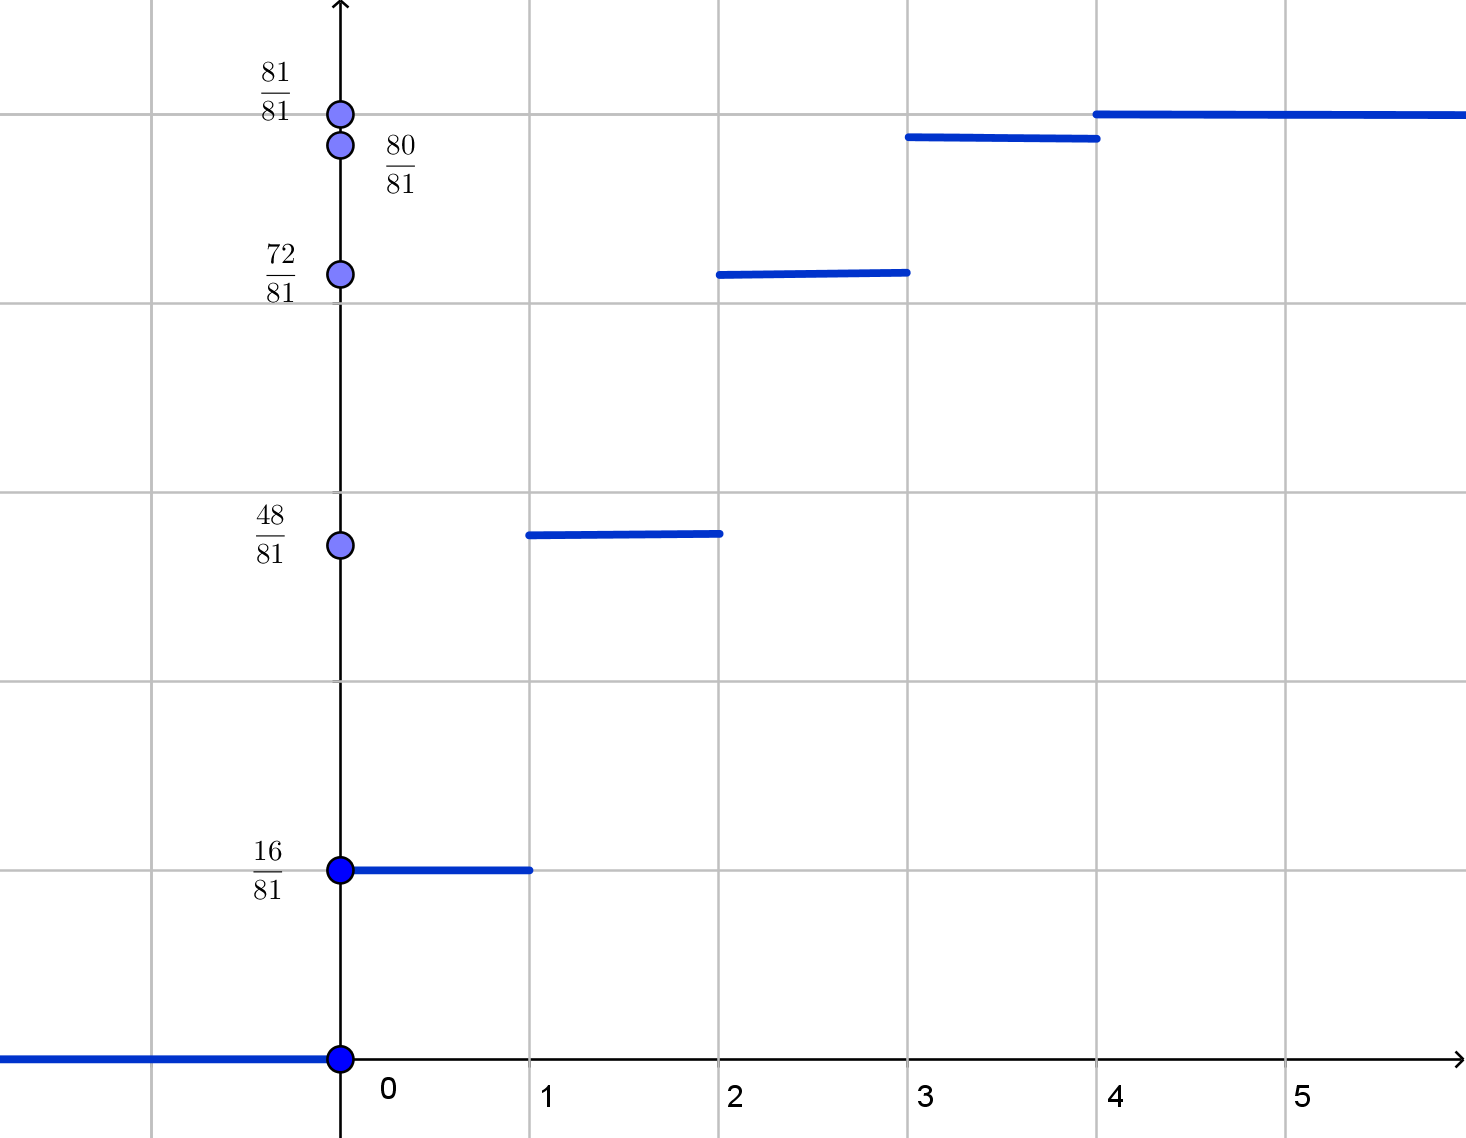
\includegraphics[width=80mm]{images/kr1_2017_3.png}
    }
    \caption{Функция распределения}
    \label{cdf_kr2017}
\end{figure}

\item Все вероятности посчитаны, видим, что наибольшая достигается при $\xi=1$.
\item $\E(X) = np = \frac{4}{3} $, $ \Var(X) = npq = \frac{8}{9}$
\end{enumerate}
\item
\begin{enumerate}
\item Так как указано, что цена сметаны распределена равномерно на отерзке $[250, 1000]$, максимальное значение цены — $1000$, это и есть необходимая сумма.
\item Вспомним, что функция распределения $F(x) = \P(X \leq x)$, нужно найти такой $x$, что $ \P(X \leq x)=0.9$:
\[
0.9 = 1 - \exp({-x^{2}}) \Rightarrow \exp(-x^{2}) = 0.1 \Rightarrow -x^2 = \ln(0.1)  \Rightarrow x=  \sqrt{-\ln(0.1)}
\]
\item Взяв производную от функции распределения списка без сметаны, получим функцию плотности:
\[
f_X(x) =
\begin{cases}
2x\exp(-x^2) & x \ge 0 \\
0 & \text{иначе}
\end{cases}
\]
Найдём математическое ожидание:
\[
\int_{0}^{+\infty}2x^2\exp({-x^2}) dx = -x \exp({-x^2})\big|_0^{+\infty} + \int_{0}^{+\infty}\exp({-x^2}) dx = \frac{\sqrt{\pi}}{2}
\]
\item Математическое ожидание суммы случайных величин равно сумме математических ожиданий случайных влечин, если они существуют. Математическое ожидание от цены сметаны равно: $ \frac{1000 + 250}{2} = 625 $
Математическое ожидание списка без сметаны было найдено в предыдущем пункте, его осталось перевести в рубли. Получаем ответ: $ 625 + \frac{\sqrt{\pi}}{2} \cdot 1000 $.
\item Так как обе величины имеют абсолютно непрерывные распределения, вероятность попасть в конкретную точку равна нулю.
\end{enumerate}
\item
\begin{enumerate}
\item $\P(\text{детектор показал ложь и подозреваемый лжёт}) = 0.9 \cdot 0.1 + 0.1 \cdot 0.95 = 0.185$
\item $\P(\text{невиновен}|\text{детектор показал ложь}) = \frac{0.9\cdot0.1}{0.185} = \frac{90}{185}$
\item $\P(\text{эксперт точно выявит преступника}) = (0.9)^9 \cdot 0.95$
\item $\P(\text{эксперт ошибочно выявит преступника}) = 9 \cdot 0.1 \cdot 0.9^8\cdot 0.05$
\end{enumerate}
\end{enumerate}


\subsubsection*{\hyperref[sec:kr_01_2016_2017]{2016-2017}}
\label{sec:sol_kr_01_2016_2017}

\begin{enumerate}
\item
\begin{enumerate}
\item Возможны четыре равновероятные ситуации:
\[
\P(\text{ММ}) = \P(\text{МД}) = \P(\text{ДМ}) = \P(\text{ДД}) = 1/4
\]

Посчитаем условную вероятность:
\[
\P(B \mid A) = \frac{\P(B \cap A)}{\P(A)} = \frac{\P(\text{МД, ДМ})}{\P(\text{ДМ, МД, ДД})} = \frac{2/4}{3/4} = \frac{2}{3}
\]

\item События $A$ и $B$ называются независимыми, если $\P(A \cap B) = \P(A) \cdot \P(B)$

В нашем случае: $\P(A \cap B) = \P (\text{МД, ДМ}) = 2/4$,
$\P(A) \cdot \P (B) = 3/4 \cdot 3/4$.

Следовательно, $\P(A \cap B) \neq \P(A) \cdot \P (B)$,
значит, события $A$ и $B$ не являются независимыми.
\end{enumerate}

\item Пусть событие $A_i$ означает, что $i$-ый узел системы дал сбой,
а событие $B_N$, что вся система дала сбой.

В условии сказано, что $\P(A_i) = 10^{-6}$,
а найти нужно такое максимальное $N \in \mathbb{N}$, при котором

\[
\P(B_N) \leq \frac{1}{10^2}
\]

\begin{align*}
\P(B_N) &= \P\left(\cup_{i=1}^n A_i\right) = 1 - \P (\left(\cup_{i=1}^n A_i\right)^c) \\
&\stackrel{\text{ф-ла де Моргана}}{=} 1 - \P \left(\cup_{i=1}^N A_i^c\right) \stackrel{A_1, \ldots, A_N \text{– независ.}}{=} 1 - \P(A_1^c) \cdot \ldots \cdot \P(A_N^c) \\
&= 1 - \left(1-\frac{1}{10^6}\right)^N
\end{align*}
Чтобы найти такое максимальное $N \in \mathbb{N}$, надо решить следующее неравенство
\begin{align*}
& 1 - \left(1-10^{-6}\right)^N \leq 10^{-2} \\
& 1 - 10^{-2} \leq \left(1-10^{-6}\right)^N \\
& \ln\left(1 - 10^{-2}\right) \leq N \ln \left(1 - 10^{-6}\right) \\
& N \leq \frac{\ln\left(1 - 10^{-2}\right)}{ \ln \left(1 - 10^{-6}\right)} \approx 10050.33
\end{align*}
Значит, максимальное $N$ равно $10050$.

\item Введём обозначения для событий.
Пусть $A$ означает, что человек имеет заболевание лёгких,
а $B$, что человек работал в шахте.

В условии сказано, что $\P(B \mid A) = 0.22$, $\P(B \mid A^c) = 0.14$, $\P(A) = 0.04$.
\begin{enumerate}
\item Нужно найти
\[
\P(A \mid B) = \frac{\P(A\cap B)}{\P (B)} = \frac{\P(B|A)\P(A)}{\P(B)}
\]
Для этого с помощью формулы полной вероятности посчитаем
\[
\P (B) = \P (B \mid A) \P(A) + \P (B \mid A^c) \P (A^c) = 0.22 \cdot 0.04 + 0.14 \cdot 0.96 = 0.1432
\]
Осталось подставить значения:
\[
\P(A \mid B) = \frac{0.22 \cdot 0.04}{0.1432} \approx 0.0615
\]

\item Все необходимые значения для второго пункта у нас есть,
осталось применить формулу условной вероятности:
\begin{multline*}
\P  (A \mid B^c) =  \frac{\P(A\cap B^c)}{\P (B^c)} =  \frac{\P (B^c \cap A)}{\P(A)} \cdot \frac{\P(A)}{\P (B^c)} = \P (B^c \mid A) \cdot \frac{\P(A)}{\P (B^c)} = \\
= (1-\P (B \mid A)) \cdot \frac{\P(A)}{1-\P (B)} = (1-0.22) \cdot \frac{0.04}{1-0.1432} \approx 0.0364
\end{multline*}
\end{enumerate}
\item Введём индикатор события «Петя дал верный ответ на $i$-ый вопрос»:
\[
X_i =
\begin{cases}
1, & \text{если на } i \text{-ый вопрос теста Петя дал верный ответ} \\
0, & \text{иначе}
\end{cases}
\]

Заметим, что $X_i \sim Be\left(p = 1/5 \right)$, $X_1, \ldots, X_{17}$ – независимы,
$X = X_1 + \ldots + X_{17}$ – общее число верных ответов,
$X \sim Bin\left(n=17, p=1/5\right)$.

\begin{enumerate}
\item Наибольшее вероятное число правильных ответов $m_0$ может быть нвйдено по формуле:
\begin{enumerate}
\item[1)] если число $(n\cdot p - q)$ – не целое, где $q:=1-p$, то
\[
m_0 = [np-q] +1,
\]
\item[2)] если число  $(n\cdot p - q)$ – целое, то наиболее вероятных значений $m_0$ два:
\[
m_0' = np-q \text{ и } m_0'' = np-q+1
\]
\end{enumerate}
Итак, поскольку $np-q = 17\cdot\frac{1}{5} - \frac{4}{5} = 2.6$ – не целое, наиболее вероятное число верных ответов $m_0$ может быть найдено по формуле из пункта (1):
\[
m_0 = [np-q] +1 = [2.6] + 1 = 3
\]
\item \[\E(X) = np = 17 \cdot \frac{1}{5}=3.4\]

\[\Var(X) = npq = 17 \cdot \frac{1}{5} \cdot \frac{4}{5} = 2.72\]

\item
\begin{multline*}
\P (\text{Петя получит «отлично»}) = \P (X\geq 15) = \P (X = 15) + \P (X= 16) + \\
+ \P (X = 17) = C^{15}_{17} \cdot \left(\frac{1}{5}\right)^{15} \cdot \left(\frac{4}{5}\right)^2 + C^{16}_{17} \cdot \left(\frac{1}{5}\right)^{16} \cdot \left(\frac{4}{5}\right)^1 + C^{17}_{17} \cdot \left(\frac{1}{5}\right)^{17} \cdot \left(\frac{4}{5}\right)^0 = \\
= 136 \cdot \frac{16}{5^{17}} + 17 \cdot \frac{4}{5^{17}} + \frac{1}{5^{17}} \approx 2.94 \cdot 10^{-9}
\end{multline*}
\item Рассмотрим первый вопрос теста. Петя может выбрать первый ответ с вероятностью $1/5$, и Вася
может выбрать первый ответ с вероятностью $1/5$. Тогда они оба выберут одинаковый ответ с вероятностью $1/25$.
Вариантов ответа в каждом вопросе $5$, значит, вероятность совпадения ответа в одном вопросе равна $1/5$.
Всего вопросов 17, тогда получаем
\[
\P(\text{все ответы Пети и Васи совпадают}) = \left(\frac{1}{5}\right)^{17}
\]

\end{enumerate}
\item Введём случайную велчину $\eta$, которая означает число потенциальных покупателей, с которыми контактировал продавец оборудования. По условию задачи, $\eta$ имеет таблицу распеределения:
\begin{center}
\begin{tabular}{ccc}
\toprule
$\eta$ & $ 1 $ & $2$ \\ \midrule
$\P_{\eta}$ & $1/3$ & $2/3$ \\ \bottomrule
\end{tabular}
\end{center}
Случайная величина $\xi$ может принимать значения $0, 50000$ и $100000$
\begin{enumerate}

\item Найдём $\P (\xi = 0 )$. По формуле полной вероятности, имеем:
\begin{multline*}
\P (\xi = 0) = \P (\xi = 0 \mid \eta = 1 ) \cdot \P ( \eta = 1 ) + \P (\xi = 0 \mid \eta = 2 )  \cdot \P ( \eta = 2 )  = \\
= 0.9 \cdot \frac{1}{3} + 0.9\cdot0.9 \cdot \frac{2}{3} = 0.84
\end{multline*}

\item Найдём $\P (\xi = 50000 )$ и $\P (\xi = 100000 )$ :
\begin{multline*}
\P (\xi = 50000 ) =  \P (\xi = 50000 \mid \eta = 1 ) \cdot \P ( \eta = 1  ) +  \P (\xi = 50000 \mid \eta = 2 ) \cdot  \P ( \eta = 2 )  = \\
= 0.1 \cdot \frac{1}{3} + 2 \cdot 0.1 \cdot 0.9 \cdot \frac{2}{3} = 0.15(3)
\end{multline*}
\begin{multline*}
\P (\xi = 100000 ) =  \P (\xi = 100000 \mid \eta = 1 ) \cdot \P ( \eta = 1 ) +  \P (\xi = 100000 \mid \eta = 2 ) \cdot  \P ( \eta = 2  )  =  \\
= 0 \cdot \frac{1}{3} + 0.1\cdot 0.1  \cdot \frac{2}{3} = 0.00(6)
\end{multline*}
Таблица распределения случайной величина $\xi$ имеет вид:

\begin{center}
\begin{tabular}{cccc}
\toprule
$\xi$ & $ 0 $ & $5000$ & $100000$ \\ \midrule
$\P_{\xi}$ & $0.84$ & $0.15(3)$ & $0.00(6)$ \\ \bottomrule
\end{tabular}
\end{center}

Тогда функция распределения случайной величины $\xi$ имеет вид:
\[
F_{\xi} (X) =
\begin{cases}
0 & \text{при } x<0 \\
0.84 & \text{при } 0 \leq x < 50000 \\
0.84 + 0.15(3) & \text{при } 50000
\leq x < 100000 \\
1 & \text{при } x > 100000
\end{cases}
\]
Опр.: $F_{\xi} = \P (\xi \leq x ), x \in \mathbb{R}$
\item \[\E (X) = 0 \cdot 0.84 + 50000 \cdot 0.15(3) + 100000 \cdot 0.00(6) = 8333.(3)	\]
\begin{multline*}
\Var(X) = (0 - 8333.(3))^2 \cdot 0.84 + (50000-8333.(3))^2 \cdot 0.15(3) + \\
+ (100000 - 8333.(3))^2 \cdot 0.00(6) = 380555555.(5)
\end{multline*}
\end{enumerate}
\item
\begin{enumerate}
\item $ f_{\xi} (x)=
\begin{cases}
\frac{1}{b} & \text{при } x \in [0, b] \\
0 & \text{при } x \notin [0, b]
\end{cases}
$
\item  Известно, что если $\xi \sim U[a, b]$, то $\E (\xi) = \frac{a+b}{2}$. Стало быть, из уравнения $\E (\xi) = 1$ получаем $\frac{b}{2} = 1$,  то есть $b=2$.
\item Известно, что если $\xi \sim U[a, b]$, то $\Var (\xi) = \frac{(b-a)^2}{12}$. Значит, $\Var (\xi) = \frac{2^2}{12} = \frac{1}{3}$
\item Воспользуемся формулой $\P (\xi \in B ) = \int_B f_{\xi} (x) dx$. Имеем:
\[
\P (\xi > 1 ) = \P (\xi \in (1, + \infty) ) = \int_{1}^{+ \infty} f_{\xi} (x) dx = \int_{1}^{2} \frac{1}{2} dx = \frac{1}{2}
\]
\item Требуется найти такое минимальное число $q_{0.25}$, что $\int_{-\infty}^{q_{0.25}} f_{\xi} (x) dx = 0.25$. Итак:
\[
\int_{-\infty}^{q_{0.25}} f_{\xi} (x) dx = 0.25 \Leftrightarrow \int_{-\infty}^{q_{0.25}} \frac{1}{2} dx = 0.25 \Leftrightarrow \frac{1/2}{q_{0.25}} = 0.25 \Leftrightarrow
\]
\[
q_{0.25} = 2 \cdot 0.25 = 0.5
\]
\item
\begin{multline*}
\E [ (\xi - \E(\xi))^{2017} ] = \int_{-\infty}^{+\infty} (x- \E(\xi) )^{2017} \cdot f_{\xi} (x) dx = \int_{-\infty}^{+\infty} (x-1)^{2017} f_{\xi} (x) dx = \\
= \int_{0}^{2} (x-1)^{2017} \cdot \frac{1}{2} dx = \frac{(x-1)^{2018}}{2018} \cdot \frac{1}{2} \bigg\rvert_{x=0}^{x=2} =0
\end{multline*}
\item $F_{\xi} (x) =
\begin{cases}
0 & \text{при } x < 0 \\
\frac{x}{2} & \text{при } 0 \leq x \leq 2 \\
1 & \text{при } x > 2
\end{cases}
$
\item Согласно условиям задачи, время до прихода 1-го поезда есть $\xi$; время до прихода 2-го поезда равно $\xi + b$; время до прихода 3-го (заветного) поезда есть $\xi + 2b$. Таким образом, Марья Ивановна в среднем ожидает «своего» поезда $\E (\xi + 2b) = 1 + 2b = 1 + 2 \cdot 2 = 5 $ минут. При этом $\Var (\xi + 2b) = \Var (\xi) = 1/3$
\item[к)] Пусть $\tau$ – наименьший номер поезда без «подозрительных лиц». По условию задачи, таблица распределения случайной величины $\tau$ имеет вид:

\begin{center}
\begin{tabular}{cccccc}
\toprule
$\tau$ & $ 1 $ & $2$ & $3$ & $4$ & \ldots \\ \midrule
$\P_{\tau}$ & $1/4$ & $3/4\cdot1/4$ & $(3/4)^2 \cdot 1/4$ & $(3/4)^3 \cdot 1/4$ & \ldots\\ \bottomrule
\end{tabular}
\end{center}

То есть случайная величина $\tau$ имеет геометрическое распределение с параметром $p=1/4$ $(\tau \sim G(p=1/4))$.

Несложно сообразить, что время ожидания Глафирой Петровной «своего» поезда составляет: $\eta := \xi + b(\tau- 1)$. Стало быть, $\E (\eta) = \E (\xi) + b \cdot (\E(\tau)-1)  = 1 + 2 \cdot (4-1) = 7$ минут.

Здесь мы воспользовались тем фактом, что если $\eta \sim G(p)$, то $\E (\eta) = 1/p$
\item[и)] Найдём теперь вероятность $\P (\eta \geq 5 )$. Для нахождения искомой вероятности воспользуемся формулой полной вероятности:
\[
	\P (\eta \geq 5 ) = \P(\eta \geq 5, \tau < 3) +\P(\eta \geq 5, \tau = 3)+\P(\eta \geq 5, \tau > 3)
\]

Если Глафира уехала на первом или втором поезде,
то ждать больше 5 минут она не могла, то есть $\P(\eta \geq 5, \tau <3)=0$.

Если Глафира уехала на третьем поезде, то чтобы ждать больше пяти минут,
ей нужно ждать первый поезд больше минуты,
то есть $\P(\eta \geq 5, \tau = 3)=0.5 \P(\tau = 3)$.

Если Глафира уехала на четвертом поезде или позже, то она точно ждала больше 5 минут,
$\P(\eta \geq 5, \tau >3)=\P(\tau>3)$.

\[
\P(\eta \geq 5) = 0.5\P(\tau = 3) + \P(\tau > 3) = 0.5 \cdot (3/4)^2 \cdot (1/4) + (3/4)^3 = 63 / 128
\]

\end{enumerate}
\item Пусть $\xi$ — случайная величина, обозначающая число остановок лифта. Предствим её в виде суммы $\xi = \xi_2 + \ldots + \xi_{10}$, где $\xi_i$ — индикатор
того, что лифт остановился на $i$-ом этаже, то есть
\[
\xi_i = \begin{cases}
1 & \text{если лифт остановился} \\
0 & \text{иначе}
\end{cases}
\quad \forall i = 2, \ldots, 10
\]
Найдём соответсвующие вероятности:
\[
\P(\xi_i = 0) = \left(\frac{8}{9}\right)^9
\]
\[
\P(\xi_i = 1) = 1 - \P(\xi = 0) = 1 - \left(\frac{8}{9}\right)^9
\]
Тогда $\E(\xi_i) = \P(\xi_i = 0) \cdot 0 + \P(\xi_i = 1) \cdot 1 = 1 - \left(\frac{8}{9}\right)^9$, и в итоге получаем:
\[
\E(\xi) = 9 \cdot \E(\xi_i) = 9 \cdot \left(1 - \left(\frac{8}{9}\right)^9\right)
\]
\end{enumerate}

\subsubsection*{\hyperref[sec:kr_01_2015_2016]{2015-2016}}
\label{sec:sol_kr_01_2015_2016}

\begin{enumerate}
\item
\begin{enumerate}
\item[$\alpha$)] Найдём вероятности каждого события:
$\P(A) = 1/2$, $\P(B) = 1/2$, $\P(C) = 1/2$.

Проверим попарную независимость:
\begin{itemize}
\item $\P(A \cap B) = 1/4$, $\P(A) \cdot \P(B) = 1/2 \cdot 1/2 = 1/4$
\item $\P(A \cap C) = 1/4$, $\P(A) \cdot \P(C) = 1/2 \cdot 1/2 = 1/4$
\item $\P(B \cap C) = 1/4$, $\P(B) \cdot \P(C) = 1/2 \cdot 1/2 = 1/4$
\end{itemize}
Значит, события попарно независимы.
\item[$\beta$)] События $A_1, A_2, A_3$ называются независимыми в совокупности,
если $\P(A_1 \cap A_2 \cap A_3) = \P(A_1) \cdot \P(A_2) \cdot \P(A_3)$.

В нашем случае: $\P(A \cap B \cap C) = 0$, $ \P(A) \cdot \P(B) \cdot \P(C) = (1/2)^3$,
следовательно, события не являются независимыми в совокупности.
\end{enumerate}

\item
\begin{enumerate}
\item[$\alpha$)] Воспользуемся формулой полной вероятности:
\begin{align*}
\P(\text{выпала «6»}) &= \P(\text{выпала «6»} \mid \text{взят белый кубик}) \cdot \P(\text{взят белый кубик}) \\
&+ \P(\text{выпала «6»} \mid \text{взят красный кубик}) \cdot \P(\text{взят красный кубик}) \\
&= \frac{1}{6} \cdot \frac{1}{2} + \frac{1}{3} \cdot \frac{1}{2} = \frac{1}{4}
\end{align*}
\item[$\beta$)] Воспользуемся формулой условной вероятности и результатом предыдущего пункта:
\begin{align*}
\P(\text{взят красный кубик} \mid \text{выпала «6»}) &= \frac{\P(\text{взят красный кубик} \cap \text{выпала «6»})}{\P(\text{выпала «6»})}  \\
&= \frac{\frac{1}{2}\cdot \frac{1}{3}}{\frac{1}{4}} = \frac{2}{3}
\end{align*}
\end{enumerate}

\item
\begin{enumerate}
\item[$\alpha$)] Совместное распределение имеет вид:
\begin{center}
\begin{tabular}{@{}lllllll@{}}
\toprule
$\eta$ $\backslash$ $\xi$ & $1$                            & $2$                            & $3$                            & $4$                            & $5$                            & $6$                            \\ \midrule
$1$           & $\frac{2}{15}\cdot\frac{1}{6}$ & $\frac{2}{15}\cdot\frac{1}{6}\mbox{*}$  & $\frac{2}{15}\cdot\frac{1}{6}\mbox{*}$   & $\frac{2}{15}\cdot\frac{1}{6} \mbox{*}$   & $\frac{2}{15}\cdot\frac{1}{6} \mbox{*}$   & $\frac{1}{3}\cdot\frac{1}{6} \mbox{*}$   \\
$2$           & $\frac{2}{15}\cdot\frac{1}{6}$ & $\frac{2}{15}\cdot\frac{1}{6}$ & $\frac{2}{15}\cdot\frac{1}{6}\mbox{*}$   & $\frac{2}{15}\cdot\frac{1}{6}\mbox{*}$   & $\frac{2}{15}\cdot\frac{1}{6}\mbox{*}$   & $\frac{1}{3}\cdot\frac{1}{6} \mbox{*}$   \\
$3$           & $\frac{2}{15}\cdot\frac{1}{6}$ & $\frac{2}{15}\cdot\frac{1}{6}$ & $\frac{2}{15}\cdot\frac{1}{6}$ & $\frac{2}{15}\cdot\frac{1}{6} \mbox{*}$   & $\frac{2}{15}\cdot\frac{1}{6} \mbox{*}$   & $\frac{1}{3}\cdot\frac{1}{6} \mbox{*}$   \\
$4$           & $\frac{2}{15}\cdot\frac{1}{6}$ & $\frac{2}{15}\cdot\frac{1}{6}$ & $\frac{2}{15}\cdot\frac{1}{6}$ & $\frac{2}{15}\cdot\frac{1}{6}$ & $\frac{2}{15}\cdot\frac{1}{6} \mbox{*}$ & $\frac{1}{3}\cdot\frac{1}{6} \mbox{*}$   \\
$5$           & $\frac{2}{15}\cdot\frac{1}{6}$ & $\frac{2}{15}\cdot\frac{1}{6}$ & $\frac{2}{15}\cdot\frac{1}{6}$ & $\frac{2}{15}\cdot\frac{1}{6}$ & $\frac{2}{15}\cdot\frac{1}{6}$ & $\frac{1}{3}\cdot\frac{1}{6} \mbox{*}$   \\
$6$           & $\frac{2}{15}\cdot\frac{1}{6}$ & $\frac{2}{15}\cdot\frac{1}{6}$ & $\frac{2}{15}\cdot\frac{1}{6}$ & $\frac{2}{15}\cdot\frac{1}{6}$ & $\frac{2}{15}\cdot\frac{1}{6}$ & $\frac{1}{3}\cdot\frac{1}{6}$ \\ \bottomrule
\end{tabular}
\end{center}
\item[$\beta$)] $\P(\text{выиграет белый кубик}) = (6 + 5 + 4 + 3 + 2) \cdot \frac{2}{15}\cdot\frac{1}{6} + 1 \cdot \frac{1}{3}\cdot\frac{1}{6} = \frac{1}{2}$.

Значит, Пете безразлично, какой кубик брать.
\item[$\gamma)$] $F_{\zeta}(x) = \P(\zeta \leq x)$

Выпишем таблицу распределения случайной величины $\zeta$:

\begin{center}
\begin{tabular}{@{}lcccccc@{}}
\toprule
$\zeta$     & $1$                              & $2$                                      & $3$                                      & $4$                                      & $5$                                      & $6$                                                                              \\ \midrule
$\P(\cdot)$ & $\frac{2}{15} \cdot \frac{1}{6}$ & $\frac{2}{15} \cdot \frac{1}{6} \cdot 3$ & $\frac{2}{15} \cdot \frac{1}{6} \cdot 5$ & $\frac{2}{15} \cdot \frac{1}{6} \cdot 7$ & $\frac{2}{15} \cdot \frac{1}{6} \cdot 9$ & $\frac{1}{3} \cdot \frac{1}{6} \cdot 6 + \frac{2}{15} \cdot \frac{1}{6} \cdot 5$ \\ \bottomrule
\end{tabular}
\end{center}

Тогда функция распределения имеет вид:
\[
F_{\zeta}(x) =
\begin{cases}
0 & x \leq 1 \\
\frac{1}{45} & 1 < x \leq 2 \\
\frac{4}{45} & 2 < x \leq 3 \\
\frac{9}{45} & 3 < x \leq 4 \\
\frac{16}{45} & 4 < x \leq 5 \\
\frac{25}{45} & 5 < x \leq 6 \\
1 & x > 6
\end{cases}
\]
\item[$\delta$)] $\E(\zeta) = \frac{2}{15} \cdot \frac{1}{6} \cdot 1 + \frac{2}{15} \cdot \frac{1}{6} \cdot 3 \cdot 2 + \frac{2}{15} \cdot \frac{1}{6} \cdot 5 \cdot 3 + \frac{2}{15} \cdot \frac{1}{6} \cdot 7 \cdot 4 + \frac{2}{15} \cdot \frac{1}{6} \cdot 9 \cdot 5 + \frac{1}{3} \cdot \frac{1}{6} \cdot 6 + \frac{2}{15} \cdot \frac{1}{6} \cdot 6 = \frac{43}{9} \approx 4.8 $
\end{enumerate}
\item Пусть $x$ — вероятность того, что мужчина честно любит петь в душе.

Распишем по формуле полной вероятности вероятность получить ответ «да»:
\begin{multline*}
P(\text{ответ «Да»}) = 1 \cdot \P(\text{выпала «6»}) + x \cdot(\P(\text{выпала «2»}) + \P(\text{выпала «3»}) +  \\
+ \P(\text{выпала «4»}) + \P(\text{выпала «5»})) = 1 \cdot \frac{1}{6} + x \cdot \frac{4}{6} \Rightarrow x = \frac{3}{4}
\end{multline*}
Тогда истинный процент «певцов» составляет $75 \%$

\item Предположим, что ваше имя — Студент (7 букв), а фамилия — Идеальный (9 букв).
\begin{enumerate}
\item[$\alpha$)] $\P(\text{напишет фаимлию правильно}) = (0.9)^9$
\item[$\beta$)] $\P(\text{ровно 2 ошибки в имени}) = C_{7}^2 \cdot 0.1^2 \cdot 0.9^5$
\item[$\gamma$)] Наиболее вероятное число ошибок — 1
\item[$\delta$)] $\P(\text{допустит хотя бы одну ошибку}) = 1 - \P(\text{не допустит ни одной ошибки}) = 1 - (0.9)^{16}$
\end{enumerate}

\item
\begin{enumerate}
\item[$\alpha$)] Из условия $\int_{0}^{1} (cy^2 + y) dy = 1$ получаем, что $c=3/2$.
\item[$\beta$)]
$F_{Y} (y) =
\begin{cases}
1 & y > 1 \\
\frac{y^3 + y^2}{2} & 0 < y \leq 1 \\
0 & y < 0
\end{cases} $
\item[$\gamma$)] $\P(Y < 0.5) = \int_{0}^{0.5} \left(\frac{3}{2} y^2 + y   \right) dy = \frac{3}{16}$
\item[$\delta$)] $F_{Y} (y) = 0.5 \Rightarrow y \approx 0.75 $
\item[$\epsilon$)] $\P(Y > 0.5 \mid Y \geq 0.25) = \frac{\P(Y > 0.5)}{\P(Y \geq 0.25)} = \frac{1 - \frac{3}{16}}{\int_{0.25}^{1} \left(\frac{3}{2} y^2 + y   \right) dy} = \frac{104}{123}$
\end{enumerate}

\item
\begin{enumerate}
\item[$\alpha$)] $\P(\text{кисточка окажется на слоне}) = \frac{1}{1.5} = \frac{2}{3}$
\item[$\beta$)] $f_{\xi, \eta}(x, y) = \frac{1}{1.5}$
\item[$\gamma$)] $f_{\xi} (x) = \int_{0}^{1} \frac{1}{1.5} dy = 1.5$

$f_{\eta}(y) = \int_{0}^{1.5} \frac{1}{1.5} dx = 1$
\item[$\delta$)] Да, поскольку $ f_{\xi} (x) \cdot f_{\eta}(y) = f_{\xi, \eta}(x, y)$
\item[$\epsilon$)] $f_{\xi+\eta} (t) = \int_{-\infty}^{+\infty} f_{\xi}(u) f_{\eta}(t-u) du $
\end{enumerate}
\end{enumerate}



\subsubsection*{\hyperref[sec:kr_01_2014_2015]{2014-2015}}
\label{sec:sol_kr_01_2014_2015}



\begin{enumerate}
\item Внимательно читайте примечание! Всего 6 возможных ситуаций, только 1 — благоприятная.
Требуемая вероятность равна $1/6$.

\item
Два события $A$ и $B$ независимы, если: $\P(AB) = \P(A) \P(B)$.

Проверим, независимы ли события $A = \{ \xi < 1/2 \} $ и  $B = \{ \eta < 1/2 \} $:

$\P(AB)$ ищется как отношение площади квадрата с вершинами в $(0,\,0)$, $(0,\,1/2)$,
$(1/2,\,1/2)$, $(1/2,\,0)$ к площади данного треугольника, то есть:
\[
\P(AB) = \frac{(1/2)^2}{1/2}= \frac{1}{2}
\]

$\P(A)$ ищется как отношение площади трапеции с вершинами в $(0,\,0)$, $(0,\,1)$,
$(1/2,\,1/2)$, $(1/2,\,0)$ к площади данного треугольника, то есть:
\[
\P(A) = \frac{(1/2)\cdot (3/2) \cdot (1/2)}{1/2}= \frac{3}{4}
\]

$\P(B)$ ищется как отношение площади трапеции с вершинами в $(0,\,0)$, $(1,\,0)$,
$(1/2,\,1/2)$, $(0,\,1/2)$ к площади данного треугольника, то есть:
\[
\P(B) = \frac{(1/2)\cdot (3/2) \cdot (1/2)}{1/2}= \frac{3}{4}
\]

\[
\P(A)\cdot \P(B) = \frac{3}{4} \cdot  \frac{3}{4} = \frac{9}{16} \ne \frac{1}{2} = \P(AB)
\]

Получается, события $A$ и $B$ зависимы.

\item
Пусть событие $A$ = \{Цель была поражена первым самолетом\},
событие $B$ = \{Цель была поражена только одним самолетом\}.
Тогда событие $AB$ = \{Первый самолет поразил цель, второй и третий — промахнулись\}.
По формуле условной вероятности:

\[\P(A|B) = \frac{\P(AB)}{\P(B)} = \frac{0.6 \cdot 0.6 \cdot 0.7}{0.6\cdot 0.6 \cdot 0.7 + 0.4 \cdot 0.4 \cdot 0.7 + 0.4 \cdot 0.6 \cdot 0.3} = \frac{0.252}{0.436} \approx 0.578\]

\item
Удобно рассуждать следующим образом: предположим, что каждая опечатка наугад
(с равными вероятностями и независимо от других опечаток) выбирает, на какую
страницу ей попасть.

\begin{enumerate}
\item Пусть $X$ — число опечаток на 13 странице. \[\P(X \geqslant 2) = 1 - \P(X=0) - \P(X=1) \]
$\P(X=0) = \left( \frac{499}{500} \right)^{400}$ — каждая из 400 опечаток не должна попасть на 13 страницу.\\
$\P(X=1) = 400\cdot\frac{1}{500}\cdot\left( \frac{499}{500} \right)^{399}$ — ровно одна опечатка (а есть 400 вариантов) должна попасть на 13 страницу, а остальные — мимо. Соответственно:
\[
\P(X \geqslant 2) = 1 - \left( \frac{499}{500} \right)^{400} - 400\cdot\frac{1}{500}\cdot\left( \frac{499}{500} \right)^{399} \approx 0.1911357
\]
Это если считать в явном виде. А если пользоваться приближением Пуассона:
\[
p(k) = \P(X = k) = \frac{\lambda^k}{k!}e^{-\lambda}
\]
неплохо бы вспомнить, что параметр $\lambda$ это математическое ожидание $X$, поэтому расчеты здесь пока оставим до лучших времен.

\item Пусть $X$ — число опечаток на 13 странице. Введем случайную величину
\[X_i =
\begin{cases}
1, & \text{если } i\text{-ая опечатка попала на 13 страницу}\\
0, & \text{если нет}
\end{cases}
\]
Тогда $X = \sum\limits_{i=1}^{400}X_i$. Рассмотрим отдельно $X_i$:

\begin{center}
\begin{tabular}{@{}ccc@{}}
\toprule
$x$         & $1$             & $0$               \\ \midrule
$\P(X=x)$ & $\frac{1}{500}$ & $\frac{499}{500}$ \\ \bottomrule
\end{tabular}
\end{center}

Так как $i$-ая опечатка наугад выбирает одну страницу из 500 и это должна быть именно 13.

Тогда:
\begin{align*}
\E(X_i) &= \frac{1}{500} = \E(X^2_i)  \\
\Var(X_i) &= \E(X^2_i) - (\E(X_i))^2 = \frac{1}{500} - \left(\frac{1}{500}\right)^2 = \frac{499}{500^2}
\end{align*}
Значит
\begin{align*}
\E(X) &= \E\left(\sum\limits_{i=1}^{400}X_i\right) = \sum\limits_{i=1}^{400}\E(X_i)  = \frac{400}{500} = 0.8 \\
\Var(X) &= \Var\left(\sum\limits_{i=1}^{400}X_i\right) = \sum\limits_{i=1}^{400}\Var(X_i) = 400\cdot\frac{499}{500^2} = 0.8\cdot\frac{499}{500}
\end{align*}

Теперь мы знаем, что $\lambda = \E(X) = 0.8$ поэтому можем вернуться к пункту (а):
\[
\P(X \geqslant 2) = 1 - \P(X=0) - \P(X=1)  = 1 - \frac{0.8^0}{0!}e^{-0.8} - \frac{0.8^1}{1!}e^{-0.8} \approx 0.19
\]

Осталось найти наиболее вероятное число опечаток на 13 странице:
\[
\P(X=k) = \frac{0.8^k}{k!}e^{-0.8} \rightarrow \max \limits_k
\]
Очевидно, что эта функция убывает по $k$, ведь с ростом $k$:\\
 $k!$ растет, а $0.8^k$ убывает. Значит наиболее вероятное число ошибок — $X = 0$

\item \href{https://en.wikipedia.org/wiki/Triskaidekaphobia}{Ох уж эти предрассудки!}
13-я страница точно такая же как и все остальные, ведь везде в решении можно просто заменить номер 13 на любой другой и ничего не изменится.

\end{enumerate}

\item
Пусть событие $A$ означает, что медицинский тест показал наличие заболевания.
Событие $B$ — заболевание на самом деле есть.

Перепишем условие задачи:

Чувствительность теста $=\P(A |B)$

Специфичность теста $=\P(A^c | B^c)$

Прогностическая сила теста $=\P(B | A)$

$\P(B) = 0.01 \Rightarrow \P(B^c) = 0.99 $

По условию, чувствительность теста равна $0.9$, тогда из формулы условной вероятности:
\[
\P(A | B) = \frac{\P(A \cap B)}{\P(B)} \Rightarrow
\P(A \cap B) = 0.9 \cdot 0.01 = 0.009
\]

При этом очевидно, что:
\[
\P(B) = \P(A \cap B) +  \P(A^c \cap B) \Rightarrow
\P(A^c \cap B) = 0.01 - 0.009 = 0.001
\]

По условию специфичность теста равна 0.95, тогда из формулы условной вероятности:
\[
\P(A^c | B^c) = \frac{\P(A^c \cap B^c)}{\P(B^c)} \Rightarrow
\P(A^c \cap B^c) =0.95 \cdot 0.99 = 0.9405
\]

При этом очевидно, что:
\[
\P(B^c) = \P(A \cap B^c) + \P(A^c \cap B^c) \Rightarrow
\P(A \cap B^c) = 0.99 - 0.9405 = 0.0495
\]

Теперь мы готовы отвечать на заданные вопросы:

\begin{enumerate}
\item
\[
\P(A) = \P(A \cap B^c) + \P(A \cap B) = 0.009+0.0495 = 0.0585
\]

\item Прогностическая сила теста:

\[
\P(B | A) = \frac{\P(A \cap B)}{\P(A) } = \frac{0.009}{0.0585} \approx 0.154
\]

Для того, чтобы повысить прогностическую силу теста, необходимо понизить
$\P(A \cap B^c) $, а для этого необходимо повысить специфичность теста.
\end{enumerate}

\item
\begin{enumerate}
\item
Должно выполняться условие нормировки:

\begin{align*}
& \int \limits_{-a}^0 1.5(x+a)^2 dx + \int \limits_0^a 1.5(x- a)^2  dx = 1   \\
& \left. 0.5(x+a)^3 \right|_{-a}^0 + \left. 0.5(x- a)^3 \right|_0^a  = 1  \\
& 0.5a^3 + 0.5a^3 = 1 \Rightarrow a = 1
\end{align*}

Теперь легко понять, как выглядит функция распределения (смотри определение функции распределения):

\[
F(x) = \begin{cases}
0, & x < 1 \\
0.5 (x+1)^3, & -1 \leqslant x <0 \\
1 + 0.5 (x-1)^3, & 0 \leqslant x < 1 \\
1, & x \geqslant 1
\end{cases}
\]

И с её помощью всё посчитать:
\begin{align*}
& P\left(X \in \left[\frac{1}{2}, 2 \right]  \right) = F(2) - F\left(\frac{1}{2} \right) =
1 - 1 +0.5^4 = 0.5^4  \\
& \E(X) = \int \limits_{-1}^0 x \cdot 1.5 (x + 1)^2 dx +  \int \limits_0^1 x \cdot 1.5 (x - 1)^2 dx \\
& = 1.5 \int \limits_{-1}^0\left( x^3 + 2x^2 + x\right) dx + 1.5 \int \limits_0^1\left( x^3 -2x^2 + x\right) dx \\
& =  \frac{3}{8} x^4 |_{-1}^0 + x^3 |_{-1}^0 + \frac{3}{4} x^2|_{-1}^0+    \frac{3}{8} x^4 |_0^1   - x^3 |_0^1 + \frac{3}{4} x^2|_0^1  = - \frac{3}{8}  + 1- \frac{3}{4} + \frac{3}{8} - 1 +\frac{3}{4} = 0
\end{align*}
А можно было заметить, что функция плотности — четная функция, поэтому сразу $\E(X) = 0$

Вычислим $\E(X^2)$:

\begin{align*}
& \E(X^2) = \int \limits_{-1}^0 x^2 \cdot 1.5 (x + 1)^2 dx +  \int \limits_0^1 x^2 \cdot 1.5 (x - 1)^2 dx \\
& = 1.5 \int \limits_{-1}^0\left( x^4 + 2x^3 + x^2\right) dx + 1.5 \int \limits_0^1\left( x^4 -2x^3 + x^2\right) dx \\
& =  \frac{3}{10} x^5 |_{-1}^0 + \frac{3}{4} x^4|_{-1}^0 + \frac{1}{2} x^3 |_{-1}^0 +  \frac{3}{10} x^5 |_0^1 - \frac{3}{4} x^4|_0^1  + \frac{1}{2} x^3 |_0^1 =  \frac{1}{10} \\
& \Var(X) = \E(X^2) - (\E(X))^2 = 0.1
\end{align*}

\item Верим, что график $F(x)$, выписанной выше, вы построить можете :)
\end{enumerate}
\item
Пусть $A = \{\text{«Лекция полезна»}\}$, $B = \{\text{«Лекция интересна»}\}$. Заметим, что лекции вообще независимы друг от друга.

\begin{enumerate}
\item Пусть $X_A$ — число полезных лекций, прослушанных Васей,  $X_B$ — число интересных лекций, прослушанных Васей. Введем случайную величину:
\[X_i =
\begin{cases}
1 & \text{если } i\text{-ая лекция была полезна}\\
0 & \text{если нет}
\end{cases}
\]

Тогда $X_A = \sum\limits_{i=1}^{30}X_i$. Рассмотрим отдельно $X_i$:

\begin{center}
\begin{tabular}{@{}ccc@{}}
\toprule
$x$         & $1$             & $0$               \\ \midrule
$\P(X=x)$ & $0.9$ & $0.1$ \\ \bottomrule
\end{tabular}
\end{center}

Вероятность $0.9$ дана. Тогда:
\begin{align*}
\E(X_i) &= 0.9 = \E(X^2_i) \Rightarrow \\
\Var(X_i) &= \E(X^2_i) - (\E(X_i))^2 = 0.9 - 0.9^2 = 0.09
\end{align*}

Значит
\begin{align*}
\E(X_A) &= \E\left(\sum\limits_{i=1}^{30}X_i\right) = \sum\limits_{i=1}^{30}\E(X_i)  = 0.9\cdot30 = 27 \\
\Var(X_A) &= \Var\left(\sum\limits_{i=1}^{30}X_i\right) = \sum\limits_{i=1}^{30}\Var(X_i) = 0.09\cdot30 = 2.7
\end{align*}

Аналогично для числа интересных лекций можем получить:
\begin{align*}
\E(X_B) &= 0.7\cdot 30 = 21 \\
\Var(X_A) &= 0.21\cdot 30 = 6.3
\end{align*}


\item Так как интересность и полезность — независимые свойства лекций, то:
\[
\P(A^c \cap B^c) = \P(A^c)\cdot \P(B^c) = 0.3\cdot0.1 = 0.03,
\]
где $A^c$ значит «не $A$».
В свою очередь:
\[
\P(A\cup B) = \P(A\cap B^c) + \P(B\cap A^c) + \P(A\cap B) = 1 - \P(A^c)\cdot \P(B^c) = 0.97,
\]
где $(A\cup B)$ значит «$A$ или $B$», а $(A\cap)B$ — «$A$ и $B$».
Аналогично, путем введения бинарной случайной величины можем получить:
\begin{align*}
& \E(X_{A^c \cap B^c}) = 0.03 \cdot  30 = 0.9 \\
& \E(X_{A\cup B}) = 0.97\cdot30 = 29.1
\end{align*}
\end{enumerate}

\item
Дано: $\E(X) = 1$, $\E(Y) = 2$, $\E(X^2) = 5$, $\E(Y^2) = 8$, $\E(XY) = -1$.

Будем использовать только свойства математического ожидания, ковариации и дисперсии, и ничего больше. Ни-че-го.

\begin{itemize}
\item  $\E(2X + Y - 4) = 2\E(X) + \E(Y) + \E(-4) = 2 + 2 - 4 = 0 $
\item $\Var(X) = \E(X^2) - (\E(X))^2 = 5 - 1 = 4 $
\item $\Var(Y) = \E(Y^2) - (\E(Y))^2 = 8 - 4 = 4 $
\item $\Cov(X, Y) = \E(XY) - \E(X)\E(Y) = -1 - 2 = -3$
\item $\Corr(X, Y) = \frac{\Cov(X, Y)}{\sqrt{\Var(X)}\sqrt{\Var(Y)}} = -\frac{3}{2\cdot 2} = -0.75$
\item $\Var(X-Y-1) = \Var(X) + \Var(Y) - 2\Cov(X, Y) = 4+4 -2(-3) = 14$
\item $\Var(X+Y+1) = \Var(X) + \Var(Y) + 2\Cov(X, Y) = 4+4+2(-3) =2 $
\item \begin{multline*}
\Cov(X-Y-1, X+Y+1)=\E((X-Y)(X+Y))-\E(X-Y)\E(X+Y) = \\
\E(X^2-Y^2) - (\E(X)-\E(Y))(\E(X) + \E(Y)) =
\E(X^2) - \E(Y^2) - ((\E(X))^2 -(\E(Y))^2)=\\
 = \Var(X)-\Var(Y) = 0
\end{multline*}
 \item $\Cov(X-Y-1, X+Y+1)=0 \Rightarrow \Corr(X-Y-1, X+Y+1) = 0 $
\end{itemize}

\item Найдём частные распределения $Y$ и $Y^2$:
\begin{center}
\begin{tabular}{cccc}
\toprule
 & $X=1$ & $X=2$ & $\sum$ \\ \midrule
$Y=-1$ & $0.1$ & $0.2$ & $0.3$ \\
$Y=0$ & $0.2$ & $0.3$ & $0.5$ \\
$Y=1$ & $0$ & $0.2$ & $0.2$ \\
$\sum$ & $0.3$ & $0.7$ & \\ \bottomrule
\end{tabular}
\end{center}

\begin{center}
\begin{tabular}{@{}cccc@{}}
\toprule
$y$         & $-1$             & $0$      & $1$         \\ \midrule
$\P(Y=y)$ & $0.3$ & $0.5$  & $0.2$\\ \bottomrule
\end{tabular}
\end{center}

Так как $Y^2$ может принимать только значения 0 или 1:

\begin{center}
\begin{tabular}{@{}ccc@{}}
\toprule
$y^2$         & $0$             & $1$               \\ \midrule
$\P(Y^2 = y^2)$ & $0.5$ & $0.5$ \\ \bottomrule
\end{tabular}
\end{center}
А ковариация:
 \begin{multline*}
 \Cov(X, Y) = \E(XY) - \E(X)\E(Y) =
 ((-1)\cdot 1\cdot0.1 + (-1)\cdot2 \cdot 0.2 + 1\cdot2\cdot 0.2) -\\
 - (0.3\cdot1 + 0.7 \cdot 2)\cdot(0.3\cdot(-1) + 0.1\cdot 0.2) = 0.07
\end{multline*}

Так как $\Cov(X, Y) \ne 0$ — величины зависимы

\item Бонусная задача

Предположим, что правильный ответ 0.25. Но это невозможно, потому что вариантов ответа 0.25 — два (1 и 4), значит ответ 0.5 тоже был бы правильный. Предположим, что правильный 0.5. Тогда 0.25 тоже правильный — таких вариантов два из четырех, значит вероятность попасть в 0.25, выбрав ответ наугад, равна 0.5. Ответ 0.6, очевидно, неверен, потому что вероятность попасть в него равна 0.25. \\
\textbf{Правильный ответ:} 0
\end{enumerate}



\subsubsection*{\hyperref[sec:kr_01_2013_2014]{2013-2014}}
\label{sec:sol_kr_01_2013_2014}

\begin{enumerate}
\item Введём обозначения:
\begin{itemize}
\item $\P(\text{В} | \text{A}^{c} \cap \text{М}^{c}) = 0.18$ — Вася пришёл, а девушки — нет
\item $\P(\text{В} | \text{A} \cap \text{М}) = 0.9$ — пришли и Вася, и девушки
\item $\P(\text{В} | \text{A}^{c} \cap \text{М}) = 0.54$ — Вася пришёл, если пришла только Маша
\item $\P(\text{В} | \text{A} \cap \text{М}^{c}) = 0.36$ — Вася пришёл, если пришла только Алёна
\item $\P(\text{М}) = 0.4$ — Маша пришла на лекцию
\item $\P(\text{А}) = 0.6$ — Алёна пришла на лекцию
\end{itemize}
\begin{enumerate}
\item Используя формулы Байеса и полной вероятности, получим:
\[
\P(\text{A} | \text{В} ) = \frac{\P(\text{A} \cap \text{В})}{\P(\text{В})}
\]
В числителе:
\begin{multline*}
\P(\text{В} | \text{A}) \cdot \P(\text{А}) = P(\text{В} | \text{A} \cap \text{М}) \cdot \P(\text{А}) \cdot \P(\text{М}) + \P(\text{В} | \text{A} \cap \text{М}^{c}) \cdot \P(\text{А}) = \cdot \P(\text{М}^{c}) \\
= 0.9 \cdot 0.4 \cdot 0.6 + 0.36 \cdot 0.6 \cdot 0.6 = 0.3456
\end{multline*}
А в знаменателе:
\begin{multline*}
\P(\text{В} | \text{A}^{c} \cap \text{М}^{c}) \cdot \P(\text{A}^{c} \cap \text{М}^{c})+\P(\text{В} | \text{A} \cap \text{М}) \cdot \P(\text{A} \cap \text{М}) + \P(\text{В} | \text{A}^{c} \cap \text{М}) \cdot \P(\text{A}^{c} \cap \text{М})+ \\
+  \P(\text{В} | \text{A} \cap \text{М}^{c}) \cdot \P(\text{A} \cap \text{М}^{c}) = 0.18 \cdot 0.6 \cdot 0.4 + 0.9 \cdot 0.4 \cdot 0.6 + \\
+ 0.54 \cdot 0.4 \cdot 0.4 + 0.36 \cdot 0.6 \cdot 0.6 = 0.4752
\end{multline*}
Ответ:
\[
\P(\text{A} | \text{В} ) = \frac{\P(\text{A} \cap \text{В})}{\P(\text{В})} = \frac{0.3456}{0.4752}  =0.(72)
\]

\item Необходимо найти
\[
\P(\text{М} | \text{В}) = \frac{\P(\text{М} \cap \text{В})}{\P(\text{В})}
\]
Знаменатель этой дроби посчитан в предыдущем пункте, посчитаем числитель:
\begin{multline*}
\P(\text{М} \cap \text{В}) = \P(\text{В} | \text{М}) \cdot \P(\text{М}) = P(\text{В} | \text{М} \cap \text{А}) \cdot \P(\text{А}) \cdot \P(\text{М}) + \\
+ \P(\text{В} | \text{A}^{c} \cap \text{М}) \cdot \P(\text{А}^{c})  \cdot \P(\text{М}) = 0.9 \cdot 0.4 \cdot 0.6 + 0.54 \cdot 0.4 \cdot 0.4 = 0.3024
\end{multline*}
Ответ:
\[
\P(\text{М} | \text{В}) = \frac{\P(\text{М} \cap \text{В})}{\P(\text{В})} = \frac{0.3024}{0.4752} = 0.(63)
\]
Если Вася на лекции, вероятность застать на ней Алёну выше.
\end{enumerate}


\item $\P(X = 5) = C_{100}^5 0.002^5 0.998^{95}$,

$\E(X) = 0.2$,

$\Var(X) = 0.2\cdot 0.998$,

наиболее вероятно событие $X = 0$.
\item $c = 1/2$,
$\P(X \in [\ln 0.5,\ln 4]) = 5/8$,
$\E(X) = 0$,
$\Var(X)=2$,
$\E(X^{2k+1})=0$,
$\E(X^{2k})=(2k)!$
\item
\begin{enumerate}
\item $\E(Y - 2X - 3) = \E(Y) - 2 \E(X) - 3 = 0$

$\Var(Y - 2X - 3) = \Var(Y) + 4\Var(X) - 2\Cov(Y, 2X) = 16$

$\Cov(X, Y) = \Corr(X,Y) \cdot \sqrt{\Var(X) \cdot \Var(Y)} = 6$
\item $\Corr(Y - 2X - 3, X) = \frac{\Cov(Y, X) - 2 \Var(X)}{\sqrt{\Var(Y - 2X - 3) \cdot \Var(X)}} = -1$.
\item Корреляция равна $-1$, значит, есть линейная взаимосвязь между переменными.
Пусть $Y+ a X = b$, тогда $\Var(Y+ a X)=0$, $\E(Y) = -a + b =1 $.
Решая уравнения, находим, что $a=-2/3, b=1/3$.
\end{enumerate}

\item \begin{enumerate}
\item Таблицы распределения имеют вид:
\begin{center}
\begin{tabular}{@{}cccc@{}}
\toprule
$x$         & $-1$  & $0$   & $1$   \\ \midrule
$\P(X=x)$ & $0.3$ & $0.3$ & $0.4$ \\ \bottomrule
\end{tabular}
\hspace{1cm}
\begin{tabular}{@{}ccc@{}}
\toprule
$y$         & $-1$  & $1$   \\ \midrule
$\P(Y=y)$ & $0.5$ & $0.5$ \\ \bottomrule
\end{tabular}
\end{center}

\item
\begin{multline*}
\Cov(X, Y) = \E(XY) - \E(X) \E(Y)  = (-1)\cdot (-1) \cdot 0.1 + (-1) \cdot 0 \cdot 0.2 + \\
+ (-1) \cdot 1 \cdot 0.2 + 1 \cdot (-1) \cdot 0.2 + 1 \cdot 0 \cdot 0.1 + 1 \cdot 1 \cdot 0.1 -
0.1 \cdot 0 = -0.1
\end{multline*}
\item Да, поскольку если случайные величины независимы, то их ковариция равна нулю.
\item Условное распределение:
\begin{center}
\begin{tabular}{@{}cccc@{}}
\toprule
$X|Y=-1$    & $-1$  & $0$   & $1$   \\ \midrule
$\P(\cdot)$ & $0.2$ & $0.4$ & $0.4$ \\ \bottomrule
\end{tabular}
\end{center}
\item $\E(X | Y = -1) = -1 \cdot 0.2 + 0 \cdot 0.4 + 1 \cdot 0.4 = 0.2$
\end{enumerate}
\end{enumerate}




\subsubsection*{\hyperref[sec:kr_01_2012_2013]{2012-2013}}
\label{sec:sol_kr_01_2012_2013}

\begin{enumerate}
\item
\begin{enumerate}
\item $\P(A)=0.8\cdot 0.3+0.7\cdot 0.2=0.38$
\item $\P(B)=0.9$
\item $\P(C|A)=\frac{0.3\cdot 0.8}{0.38}=0.632$
\item $\P(C|D)=\frac{0.3\cdot (0.9\cdot 0.8+0.1\cdot 0.2)}{0.9\cdot 0.38+0.1\cdot (1-0.38)}=0.55$
\end{enumerate}
\item Это была задачка-неберучка!
\item
\begin{enumerate}
\item $1$
\item $\E(X)=45/28\approx 1.61$, $\E(X^2)=93/35\approx 2.66$, $\Var(X)=291/3920\approx 0.07$
\item $37/56\approx 0.66$
\item $F(x)=\begin{cases} 0,\, x<1 \\
\frac{x^3-1}{7},\, x\in [1;2] \\
1,\, x>1 \end{cases}$
\end{enumerate}
\item
\begin{enumerate}
\item $a=0.1$
\item $\P(X>-1)=0.7$, $\P(X>Y)=0.1$
\item $\E(X)=-0.2$, $\E(X^2)=2$
\item $\Corr(X,Y)=0.117$
\end{enumerate}
\item
\begin{enumerate}
\item Правильные: $\E(X)=10$, $\Var(X)=9$, неправильные: $\E(Y)=9$, $\Var(Y)=0.9$
\item Наиболее вероятное число укусов равно математическому ожиданию
\item Лучше идти к неправильным пчёлам, так как $\P(X\leq 2)<\P(Y\leq 2)$.
\end{enumerate}
\end{enumerate}

% !TEX root = ../probability_hse_exams.tex
\thispagestyle{empty}
\section{Решения контрольной номер 1. ИП}


\subsection[2019-2020]{\hyperref[sec:kr_01_ip_2019_2020]{2019-2020}}
\label{sec:sol_kr_01_ip_2019_2020}

\begin{enumerate}
  \item xxx
  \item xxx
  \item xxx
  \item xxx
  \item xxx
\end{enumerate}


\subsection[2018-2019]{\hyperref[sec:kr_01_ip_2018_2019]{2018-2019}}
\label{sec:sol_kr_01_ip_2018_2019}

\begin{enumerate}

\item Воспользуемся методом первого шага. Дерево игры выглядит так (в вершинах — длительность сответствующей подыгры, а на концах ветвей — доля разбавленных пинт среди тех, что Джо помнит):
\begin{center}
\begin{tikzpicture} \node {$a$} child {node {1} edge from parent node[left] {Р} node[right] {}}
child {node {$b$}
child {node {1/2} edge from parent node[left] {Р}}
child {node (x) {$c$}
child {node (y) {$d$}
child {node (s) {$e$}
child {node {2/3} edge from parent node[right] {Р}}
edge from parent node[left] {НР}}
child {node {2/3} edge from parent node[right] {Р}}
edge from parent node[right] {Р}}
edge from parent node[right] {НР}}
edge from parent node[right] {НР}};
\draw [->,black] (x) .. controls +(down:1cm) and +(left:1cm) .. node[below,sloped] {НР} (x);
\draw [->,black] (s) .. controls +(up:0.1cm) and +(left:2.5cm) .. node[below,sloped] {НР} (x);
\end{tikzpicture}
\end{center}

Если первая пинта разбавлена, то игра заканчивается (разбавлены 100\% рома).
Если первая пинта не разбавлена, то, если разбавлена вторая, игра заканчивается (50\%).
Если вторая не разбавлена, и третья тоже, то это равносильно тому, что не разбавлены только две (Джо не помнит больше трех).
Если вторая не разбавлена, а третья разбавлена, возможны три случая: если четвёртая разбавлена, то игра заканчивается;
если четвёртая не разбавлена, и пятая не разбавлена, то это эквивалентно тому, что не разбавлены только две;
если четвёртая не разбавлена, а пятая разбавлена, то игра заканчивается.
Из этих соображений получаем систему уравнений:
\[
\begin{cases}a=\frac{1}{8}+\frac{7}{8}(b+1)\\
b=\frac{1}{8}+\frac{7}{8}(c+1)\\
c=\frac{1}{8}(d+1)+\frac{7}{8}(c+1)\\
d=\frac{1}{8}+\frac{7}{8}(e+1)\\
e=\frac{1}{8}+\frac{7}{8}(c+3)
\end{cases}
\]

Отсюда $a=7514/192,b=1046/24,c=146/3,d=122/3,e=136/3$.

\item Пусть
\[
Z_i=\begin{cases}1, i \mbox{-я пинта разбавлена} \\
0, \mbox{иначе}
\end{cases}
\]

Пусть с вероятностью $x_n$ последовательность случайных величин $(Z_n)$ длиной
$n$ не содержит двух единиц подряд и оканчивается нулём, а с вероятностью $y_n$ —
не содержит двух единиц подряд и оканчивается единицей.

Пусть на последнем месте $(Z_n)$ стоит единица. Это может произойти с вероятностью
$1/2$. При этом перед последней единицей может стоять любая последовательность
длиной $n-1$, оканчивающаяся нулём. Значит, $y_n=0.5x_{n-1}$.

Пусть на последнем месте $(Z_n)$ стоит нуль. Это может произойти с вероятностью
$1/2$. При этом перед последним нулём может стоять любая последовательность длиной
$n-1$. Значит, $x_n=0.5(x_{n-1}+y_{n-1})$.

Таким образом, получена следующая разностная система:
\[
\begin{cases}x_n=0.5(x_{n-1}+y_{n-1})\\
y_n=0.5x_{n-1}
\end{cases}
\]

Более того, можно поставить задачу Коши. Так как $(Z_2)$ может равновероятно
иметь одну из 4 реализаций $(11, 10, 01, 00)$, из которых не содержат двух единиц
подряд и оканчиваются на 0 две, то $x_2=1/2$. Аналогично, $y_2=1/4$. Решив задачу
Коши, найдем формулы для $x_n$, $y_n$. Ответом будем число $x_{100}+y_{100}$.

\item
\begin{enumerate}
\item Оптимальная стратегия для Али-Бабы состоит в чередовании открытия двух
диагонально противоположных и двух соседних монет.

Изначально имеется только четыре варианта расположения монет:
\begin{center}
\begin{tikzpicture}[every node/.style={draw}]
\path[yshift=1.5cm,rectangle] (-6,0) node(a1){О} (-5,0) node(a2){Р} (-5,1) node(a3){О} (-6,1) node(a4){О};
\filldraw[fill=black] (a1) -- (a2) -- (a3) -- (a4) -- (a1);
\path[yshift=1.5cm,rectangle] (-4,0) node(a1){Р} (-3,0) node(a2){Р} (-3,1) node(a3){О} (-4,1) node(a4){О};
\filldraw[fill=black] (a1) -- (a2) -- (a3) -- (a4) -- (a1);
\path[yshift=1.5cm,rectangle] (-2,0) node(a1){Р} (-1,0) node(a2){О} (-1,1) node(a3){Р} (-2,1) node(a4){О};
\filldraw[fill=black] (a1) -- (a2) -- (a3) -- (a4) -- (a1);
\path[yshift=1.5cm,rectangle] (0,0) node(a1){Р} (1,0) node(a2){Р} (1,1) node(a3){Р} (0,1) node(a4){О};
\filldraw[fill=black] (a1) -- (a2) -- (a3) -- (a4) -- (a1);
\end{tikzpicture}
\end{center}

На первом ходе Али делает двух орлов на одной диагонали. Всего возможно восемь
случаев (по две диагонали в каждом из начальных вариантов). Из восьми равновозможных
случаев два приводят к успеху. При этом, если успех не достигнут, можно получить в
итоге только две комбинации орлов и решек (левую — в четырёх случаях, правую — в двух):
\begin{center}
\begin{tikzpicture}[every node/.style={draw}]

\path[yshift=1.5cm,rectangle] (-2,0) node(a1){О} (-1,0) node(a2){Р} (-1,1) node(a3){О} (-2,1) node(a4){О};
\filldraw[fill=black] (a1) -- (a2) -- (a3) -- (a4) -- (a1);
\path[yshift=1.5cm,rectangle] (0,0) node(a1){Р} (1,0) node(a2){О} (1,1) node(a3){Р} (0,1) node(a4){О};
\filldraw[fill=black] (a1) -- (a2) -- (a3) -- (a4) -- (a1);
\end{tikzpicture}
\end{center}

На втором ходе Али переворачивает две соседние монеты орлами вверх. При этом либо
наступает успех (8 случаев из 24), либо неуспех, приводящий к единтсвенно возможной
комбинации орлов и решек:
\begin{center}
\begin{tikzpicture}[every node/.style={draw}]
\path[yshift=1.5cm,rectangle] (-2,0) node(a1){О} (-1,0) node(a2){Р} (-1,1) node(a3){О} (-2,1) node(a4){О};
\filldraw[fill=black] (a1) -- (a2) -- (a3) -- (a4) -- (a1);
\end{tikzpicture}
\end{center}

На третьей попытке открывается или диагональ с орлами, или диагональ с орлом и решкой. В
о втором случае, очевидно, надо заменить решку на орла, и успех обеспечен. Но в первом
случае оптимально перевернуть орла и сделать 2 решки. Это даст неуспех, но Али точно
будет знать, что на четвёртой попытке монеты могут быть расположены только так:
\begin{center}
\begin{tikzpicture}[every node/.style={draw}]
\path[yshift=1.5cm,rectangle] (-2,0) node(a1){Р} (-1,0) node(a2){Р} (-1,1) node(a3){О} (-2,1) node(a4){О};
\filldraw[fill=black] (a1) -- (a2) -- (a3) -- (a4) -- (a1);
\end{tikzpicture}
\end{center}

На четвёртом ходе в любом из четырёх вариантов (Али не знает, на каком ребре решки)
нужно перевернуть обе открытые соседние монеты, тогда в двух случаях будет успех,
а в двух других -- неуспех, при котором монеты могут быть расположены только так:
\begin{center}
\begin{tikzpicture}[every node/.style={draw}]
\path[yshift=1.5cm,rectangle] (-2,0) node(a1){Р} (-1,0) node(a2){О} (-1,1) node(a3){Р} (-2,1) node(a4){О};
\filldraw[fill=black] (a1) -- (a2) -- (a3) -- (a4) -- (a1);
\end{tikzpicture}
\end{center}

Очевидно, что если на пятом ходе, открыв любую диагональ, Али перевернёт находящиеся
на ней монеты, то он гарантирует себе успех.

\item Как видим, в худшем случае потребовалось $5$ попыток.
\end{enumerate}
Источник: Кордемский, Математика изучает случайности.

\item Возьмём колоду, добавим в неё джокера. Разложим в открытую по окружности.
Джокер означает место разрыва окружности для её выкладывания в обычную колоду.
Замечаем, что джокер и четыре дамы разбивают окружность на пять случайных отрезко.
В силу симметрии ожидаемые длины этих отрезков равны и равны по $48/5$.
Значит первая дама попадается в среднем на $48/5 + 1$ месте.

\item Обозначим искомую вероятность быть в Неведении в момент $t$ значком $p_t$.
\[
p_{t+\Delta} = p_t (1-\lambda\Delta - o(\Delta))
\]

Отсюда получаем, что
\[
\frac{p_{t+\Delta} - p_t}{\Delta} = -\lambda p_t + \frac{o(\Delta)}{\Delta}
\]
Устремляем $\Delta$ к нулю и решаем получающееся дифференциальное уравнение
с начальным условием $p_0 = 1$, так как изначально Ученик находится в Неведении.

Итого:
\[
p_t = \exp(-\lambda t)
\]

\item
\[
\P(Y_4 \in [t; t+\Delta]) = C_{10}^1 \cdot \Delta \cdot C_{9}^3 t^3 (1-t)^6 + o(\Delta)
\]

Читаем вслух:
\begin{enumerate}
  \item Одна из десяти величин должна попасть в отрезок $[t; t + \Delta]$;
  \item Три из девяти оставшихся должны оказаться меньше $t$;
  \item Шесть из девяти оставших должны оказаться больше $t$;
\end{enumerate}
Вероятностью попадания двух и более величин в отрезок длины $\Delta$ пренебрегаем!
\end{enumerate}

\subsection[2017-2018]{\hyperref[sec:kr_01_ip_2017_2018]{2017-2018}}
\label{sec:sol_kr_01_ip_2017_2018}

\begin{enumerate}
\item Обозначим вероятность того, что сыр достанется Белому за $b$, если игра
начинается с его броска.

\begin{enumerate}
\item Получаем уравнение
\[
b = \frac{1}{12} + \frac{11}{12} \cdot \frac{11}{12} b
\]

Пояснение: Как Белый может победить в исходной игре? Либо сразу выкинуть 6 с вероятностью $1/12$.
Либо передать ход Серому ($11/12$), получить ход снова ($11/12$) и выиграть в продолжении игры.
Продолжение игры по сути совпадает с исходной игрой.

\item Игра продолжается до тех пор, пока кто-то не выкинет «6».
Для нахождения среднего количества бросков воспользуемся методом первого шага.

Обозначим среднее количество бросков нашей игры за $S$.
Когда Белый бросает кубик, с вероятностью $\frac{1}{12}$ игра закончится за один бросок,
а с вероятностью $\frac{11}{12}$ игра продолжится и ход перейдёт к Серому.
Но та игра, которая начнётся, когда бросать будет Серый, ничем не отличается от предыдущей,
поэтому среднее количество бросков в ней будет равно $S$.
Однако мы попадём в эту игру, «потратив» один бросок. Таким образом мы получаем:

\[
S = \frac{1}{12} \cdot 1 + \frac{11}{12}(S +1)
\]

Получается, что $S = 12$, значит игра длится в среднем 12 бросков.
\end{enumerate}

\item

\item Для того, чтобы выжить, мышам нужно ещё до начала игры договориться о стратегии,
которая позволит им с наибольшей вероятностью открыть нужные сундуки.
Если хотя бы две мыши выберут одинаковый сундук, то их в любом случае съедят.
Поэтому одной из оптимальных стратегий будет ещё до начала игры мышам договориться
и назвать левый сундук золотым, сундук посередине серебряным, а правый — платиновым.
Каждый мышонок должен открыть тот сундук, в честь которого назван необходимый ему металл.
Если внутри он обнаруживает свой металл, то он выбирает этот сундук,
если внутри находится не тот металл, мышонок открывает тот сундук,
на который указывает лежащий внутри предмет.

Например, первым заходит Микки Маус. Он открывает золотой (левый) ящик.
Если внутри лежит золото, то он выходит из комнаты. Если же внутри лежит, например, серебро,
то Микки Маус открывает сундук посередине.
Путём перебора можно посчитать, что в 4 случаях из 6 мыши смогут найти нужный металл,
поэтому вероятность выигрыша при данной стратегии равна $\frac{2}{3}$.

\item
\begin{enumerate}
  \item Обозначим буквой $X$ количество детей в случайной семье.
  Можно просуммировать ряд $\E(X) = 1\cdot 0.5 + 2\cdot 0.5^2 + 3\cdot 0.5^3 + \ldots$. 
  А можно воспользоваться методом первого шага и заметить, что либо первой рождается девочка 
  и мышиная семья больше не заводит мышат, либо рождается мальчик и семья ситуация превратилась в первоначальную
  плюс один ребёнок.

  \[
  \E(X) = 0.5 \cdot 1 + 0.5 \cdot (1 + \E(X))  
  \]
  Находим, $\E(X)=2$.
  \item В мышиной стране много семей. Занумеруем семьи. Обозначим буквой $X_i$ число детей в $i$-ой семье.
  Тогда доля $D$ — это суммарное количество мальчиков делить на суммарное количество детей:

  Получаем
  \[
  \frac{(X_1 - 1) + (X_2 - 2)+ \ldots + (X_n - 1)}{X_1 + X_2 + \ldots +X_n} = 1 - \frac{n}{\sum_{i=1}^n X_i}  
  \]

  Основной смысл математического ожидания $\E(X_i)$ — это среднее выборочное при большом количестве повторений опыта.

  Следовательно, $\frac{\sum_i X_i}{n} \to \E(X_i)=2$. И стало быть, при $n\to\infty$ получаем $D \to 1 - 1/2=1/2$.

  Интуитивный аргумент немного опасен, но всё же приведём его: вероятности рождения мальчиков и девочек равны,
  поэтому и доля будет половина. 
  Опасность аргумента состоит в том, что семьи могли бы в альтернативном условии рожать мышат по принципу: 
  пока доля мальчиков в стране не превысит 50\%. 

  \item Можно просто аккуратно суммировать ряд:
  \[
  \E(Y) = 0.5 \cdot \frac{0}{1} + 0.5^2 \cdot \frac{1}{2} + 0.5^3 \cdot \frac{2}{3} + \ldots
  \]
  
  Здесь мудрый студент может вспомнить ряд Тейлора для логарифма:
  \[
  \ln (1 + r) = r - r^2/2 + r^3/3 - r^4/4 +\ldots
  \]

  Стало быть,
  \[
  \ln (1 - 0.5) = -0.5 - 0.5^2/2 - 0.5^3/3 - 0.5^4/4  
  \]

  И исходное ожидание равно:

  \[
  \E(Y) = 1 + \ln 0.5 = 1 - \ln 2 \approx 0.31  
  \]

\item Неожиданно лёгкий вопрос, $\E(X - 1) = 2 -1=1$.
\end{enumerate}


\item Благосостояние кота Василия, положившего один гурд на вклад,
равно $m_t = 1\cdot e^{rt}$, где $r$ — процентная ставка, а $t$ — прошедшее время.

Откуда взялась экспонента?

Допустим время дискретно, а процентная ставка равна 5\% в год. 
Тогда сумма вклада каждый год домножается на $1.05$ и эволюционирует по формуле:

\[
m_t = 1 \cdot 1.05^t
\]

Но любое число можно представить в виде экспоненты, $1.05 = e^{\ln 1.05}$.

Поэтому
\[
m_t = e^{\ln 1.05 \cdot t}  = e^{rt}
\]


Момент закрытия вклада $T$ равномерно распределён на отрезке от 0 до $a$,
поэтому сумма, которую получит Василий, представима в виде $Z = e^{Y}$, где $Y \sim U[0; ra]$.
По условию, $a$ очень велико, поэтому $ra$ тоже очень велико.

Вероятность того, что первая цифра будет равна 1, равна вероятности того,
что доход Василия будет лежать в пределах от 1 до 2 гурдов, плюс вероятность того,
что он лежит в пределах от 10 до 20 гурдов и т.д.
Таким образом, можно представить эту вероятность, как:
\[
\P(N=1) = \P(e^Y \in [1;2) ) + \P(e^Y \in [10; 20) ) + \ldots
\]

Это выражение можно преобразовать таким образом:
\[
\P(N=1) = \P(Y \in [\ln 1; \ln2) ) + \P(Y \in [\ln 10; \ln 20) ) + \ldots
\]

Так как $Y$ — равномерно распределённая величина,
то $\P(Y \in [\ln 1; \ln2) ) = \frac{\ln 2 - \ln 1}{ra}$.
Для последующих слагаемых вероятность рассчитывается таким же образом.
Воспользовавшись свойством логарифма, можно заметить,
что $\frac{\ln 20 - \ln 10}{ra} = \frac{\ln 2}{ra}$.
Поэтому вероятность того, что на первом месте суммы вклада стоит единица,
равна $n\cdot \frac{\ln 2}{ra}$, где $n$ — количество слагаемых.
Путём аналогичных рассуждений получаем, что вероятность того,
что на первом месте стоит двойка, равна $n\cdot \frac{\ln 3- \ln 2}{ra}$.
Из-за того, что $a$ велико, можно считать, что число слагаемых одинаково.

На первом месте обязательно будет находиться какая-то цифра,
поэтому сумма вероятностей будет равна 1. Получаем:
\[
\dfrac{n}{ra}\left(\ln \frac{2}{1} + \ln \frac{3}{2} + \ldots + \ln \frac{10}{9}\right) = 1
\]

Таким образом $\frac{n}{ra} = \frac{1}{\ln 10}$.
Получается, что вероятность того, что на первом месте стоит единица, равна:
\[
\P (N=1) = \dfrac{\ln 2}{\ln 10}
\]

Закон распределения первой цифры выводится сложением соответствующих вероятностей.
\end{enumerate}


\subsection[2016-2017]{\hyperref[sec:kr_01_ip_2016_2017]{2016-2017}}
\label{sec:sol_kr_01_ip_2016_2017}

\begin{enumerate}
\item
\begin{enumerate}
\item Для удобства занумеруем макаронины и выделим у каждой левый и правый конец.
Взяли правый конец первой макаронины и подвязали случайной.
Взяли свободный конец только что подвязанной макаронины и подвязали случайно. И так далее.
\[
\frac{2n-2}{2n-1}\cdot \frac{2n-4}{2n-3}\cdot \ldots \cdot \frac{2}{3} \cdot 1
\]
\item Допустим, что при $n$ макаронинах в среднем образуется $e_n$ колец.
После первого соединения задача сводится к меньшему числу макаронин, важно только учесть,
образовалось ли кольцо при первом соединении:
\[
e_n = \frac{1}{2n-1}(e_{n-1}+1) + \frac{2n-2}{2n-1}e_{n-1} = e_{n-1} + \frac{1}{2n-1}
\]
\item Количество коротких колец можно разбить в сумму, $X=Z_1 + \ldots + Z_n$.
Вероятность завязывания конкретной макаронины в кольцо равна $1/(2n-1)$:
«левый конец» надо привазять именно к «правому». Значит, $\E(X)=n/(2n-1)$.
\end{enumerate}

\item
\begin{enumerate}
\item Рассмотрим обратную ситуацию: на планете есть точка, из которой связаться
хотя бы с одним пепелацем нельзя. Такое возможно, если все, кроме одного, сели
в одну полуокружность.
\[
\P(\text{есть точка без связи}) = n \cdot \left(\frac{1}{2}\right)^{n-1}
\Rightarrow \P(\text{из любой точки есть связь}) =
1 - n \cdot \left(\frac{1}{2}\right)^{n-1}
\]
\item Зафиксируем координату посадки первого пепелаца и возьмём её за точку отсчёта.
Изобразим на плоскости возможные значения центральных углов между первым пепелацем и
оставшимися и закрасим нужные участки. Получим $3/8$.
\item Зафиксируем координату посадки первого пепелаца. Обозначим центральный угол
между первым и вторым пепелацами $\alpha$. Функция плотности имеет вид:
$p(\alpha) = \frac{\sin(\alpha)}{2}$

Итог: $\int_0^{\pi/2} p(\alpha) \frac{\alpha + \pi}{2\pi} d \alpha + \int_{\pi/2}^{\pi}
p(\alpha) \frac{\pi - \alpha}{2\pi} d \alpha = \frac{\pi + 2}{4\pi}$
\end{enumerate}

\item Вспомним для начала, что площадь круга равна $\pi r^2$, а площадь сферы равна
$4\pi r^2$. Составим из маленьких треугольничков многогранник очень похожий на сферу
с единичным радиусом. Площадь этого многогранника будет примерно равна $4\pi$.
Проекция многогранника представляет собой примерно круг единичного радиуса.
Проекция имеет два слоя. С учётом обоих слоёв площадь проекции равна $2\pi$.
Значит отношение площади проекции к площади многогранника равно $1/2$.

От взаимного расположения треугольничков в пространстве ожидаемая площадь
проекции не зависит в силу аддитивности математического ожидания.

Ответ: 21 см$^2$.

\item
\begin{enumerate}
\item Мысленно отметим на окружности три точки: места ударов Брюса Ли и точку,
где схватился Чак Норрис. Можно считать, что эти три точки равномерно и независимо
распределены по окружности. Следовательно, среднее расстояние между соседними
точками равно $1/3$. Чак Норрис берёт два кусочка, слева и справа от своей точки.
Значит ему в среднем достаётся $2/3$ окружности.
\item Объявим точку, где схватился Чак Норрис нулём. Координаты двух ударов
изобразим на плоскости. Закрашиваем подходящий участок. Вероятность того, что
кусок Брюса Ли длиннее, равна $1/4$.
\end{enumerate}

\item  Рассмотрим совершенно конкурентный невольничий рынок начинающих певиц.
Певицы в хорошем настроении продаются по $V_1$, в депрессии — по $V_2$.
Получаем систему уравнений:
\[
\begin{cases}
  V_1 = 0.75 + (0.5 V_1 + 0.5 V_2) \\
  V_2 = \max_x \sqrt{x}V_1 + (1 - \sqrt{x})V_2 - x
\end{cases}
\]
Оптимизируем и получаем, $x^* = (V_1 - V_2)^2/4$. Из первого уравнения находим
$(V_1 - V_2)/2=0.75$.

\item Да. Например, такая. До общения с Джульеттой подкидывать монетку до выпадения
первого орла и запомнить число потребовавшихся подбрасываний. Пусть это будет число $X$.
Открыть равновероятно левую или правую руку Джульетты. Если открытое число больше $X$,
то сказать, что оно большее, иначе сказать, что меньшее.
\item Если $\gamma$ — вероятность самостоятельного познания Истины, а $\alpha$ —
передачи Истины отдельно в каждую из сторон, то
\[
p = \gamma + (1-\gamma) p \alpha.
\]

То есть $p=\gamma/(1-\alpha(1-\gamma))$.

Для решения второго пункта наложим на Абу Али Хусейн ибн Абдуллах ибн аль-Хасан
ибн Али ибн Сина обет молчания. Это не повлияет на вероятность постижения им Истины,
однако превратит задачу в две уже решённых :) Получаем
\[
q = \gamma + (1-\gamma)(2p\alpha - p^2\alpha^2)
\]
\end{enumerate}



\subsection[2015-2016]{\hyperref[sec:kr_01_ip_2015_2016]{2015-2016}}
\label{sec:sol_kr_01_ip_2015_2016}

\subsubsection*{Индивидуальный тур}

\begin{enumerate}
\item Сократ, эта — Η, η, дзета — Ζ, ζ, вега — нет, шо — ϸ, τ — тау, θ — тета, ξ — кси.
Греческая буква шо, ϸ, была введена Александром Македонским и ныне вышла из употребления.
По крайней мере, в греческом :) Заглавная примерно такая же, только её utf-код 03f7
не поддерживается шрифтом Linux Libertine.

\item Да. Cобытия независимы в совокупности, если для любого поднабора событий $A_1$,
\ldots, $A_k$ выполняется равенство $\P(A_1 \cap A_2 \cap \ldots \cap A_k) = \P(A_1)
\cdot \ldots \cdot \P(A_k)$. Нет.
\item $1/4$, $2/3$, $15$
\item $0$, $0.8^5\cdot 0.2$, $1-0.8^6$
\item $0.8^{10}$, $C_{10}^3 0.2^3 0.8^7$, $2$
\item $1/2$, $3/16$, $3/8$
\item
\begin{enumerate}
\item
\begin{flalign*}
F_X(x) &= \begin{cases}
0, \, x<0 \\
x^3, \, x \in [0;1] \\
1, \, x>1
\end{cases}&&
\end{flalign*}
\item $1/8$
\item $2^{-1/3}$
\item $56/63$
\item
\begin{flalign*}
F_Y(y) &= \begin{cases}
0, \, y<0 \\
1-1/y^3, \, y>0
\end{cases}&&
\end{flalign*}
\item
\begin{flalign*}
f_Y(y) &= \begin{cases}
0, \, y<0 \\
3y^{-4}, \, y>0
\end{cases}&&
\end{flalign*}

\end{enumerate}
\end{enumerate}

\subsubsection*{Командный тур}

\begin{enumerate}
\item Если отрублено 10 щупалец, значит либо был один удар породивший два новых
щупальца, либо было два удара, породивших по одному новому, а все остальные удары
не порождали новых щупалец.

Искомая вероятность равна: $8\cdot 0.5^9 \cdot 0.25^1 + C_8^2 0.5^8 0.25^2$.

Вероятность вечного боя равна нулю. Достаточно доказать, что с вероятностью один
за конечное время побеждается одноногий Кракен. А эта вероятность удовлетворяет
уравнению: $p=\frac{1}{4}p + \frac{1}{4}p^2 + \frac{1}{2} 1$. Единственный осмысленный
корень у этого уравнения — $1$.

Замечаем, что на победу над $k$-шупальцевым Кракеном уходим в $k$ раз больше ударов
в среднем чем на победу на $1$-щупальцевым. Отсюда:
\[
e_1=1 + 0.5\cdot 0 + 0.25\cdot e_1 + 0.25 \cdot 2e_1
\]
Решаем, получаем $e_1=4$ и $e_8=32$

\item Либо первая пинта разбавлена, либо первая неразбавлена, а вторая разбавлена,
то есть
\[
0.25 + 0.75\cdot 0.25 =0.4375
\]
Рисуем граф. %:

Составляем систему (индекс — количество выпитых неразбавленных пинт):
\[
\begin{cases}
e_0=\frac{1}{4} + \frac{3}{16}2 + \frac{9}{16}(2+e_2) \\
e_2=1+\frac{3}{4}e_2 + \frac{1}{4}e_0
\end{cases}
\]
Находим $e_0=64/7\approx 9$

\item Для $t>0$:
\[
\P(-\ln X \leq t)=\P(\ln X > -t)=\P(X > e^{-t})=1-e^{-t}
\]
Итого,
\[
F_{-\ln X}(t)=\begin{cases}
0, \, t < 0 \\
1-e^{-t}, \, t \geq 0
\end{cases}
\]
Из геометрических соображений легко найти $\P(XY < a)$ для $a\in (0;1)$:
\[
\P(XY < a)=a + \int_a^1 \frac{a}{x} \, dx=a-a\ln a
\]
Переходим ко второму пункту, для $t>0$:
\[
\P(-(\ln X + \ln Y) < t)=\P(XY > e^{-t})= 1-e^{-t} -t e^{-t}
\]
Итого:
\[
F_{-\ln X - \ln Y}(t)=\begin{cases}
0, \, t < 0 \\
1-e^{-t} - te^{-t}, \, t \geq 0
\end{cases}
\]
После дифференциирования получаем функцию плотности для $S=-\ln X - \ln Y$:
\[
f_S(s)=\begin{cases}
0, \, s < 0 \\
se^{-s}, \, s \geq 0
\end{cases}
\]
Приближаемся к финальной вероятности:
\[
\P(ZS > t)= \int_t^{\infty} \int_{t/s}^1  se^{-s} \, dz\, ds=
\int_t^{\infty} (s-t)\cdot e^{-s} \, ds= \ldots = e^{-t}
\]
Сравниваем результат с первым пунктом и приходим к выводу, что величина $(XY)^Z$
имеет равномерное распределение на $[0;1]$.

\item Если нанято $n$ пиратов, то вероятность, того, что в конкретный день все
работают равна $(364/365)^n$. Следовательно, ожидаемое количество праздничных дней
равно $365(1-(364/365)^n)$.

Решаем уравнение:
\[
1-(364/365)^n=100/365
\]
Получаем:
\[
n=\frac{\ln 265- \ln 365}{ \ln 364 - \ln 365}\approx 117
\]
Ожидаемое количество рабочих пирато-дней равно: $365n(364/365)^n$.

Получаем:
\[
n^*=1/(\ln 365 - \ln 364)\approx 364
\]

\item
\begin{enumerate}
\item $\P(R_{100})=1/100$ (максимум из 100 величин должен плюхнуться на сотое место),
$\P(B_{100})=1/3$ (максимум из трёх величин должен плюхнуться на второе место)
\item $\E(X)=1+\frac{1}{2} + \frac{1}{3}+\ldots + \frac{1}{100}\approx \ln 100 \approx 4.6$.
Т.к. $X=X_1+X_2+\ldots + X_{100}$ и $\E(X_i)=1/i$.
\item $\P(R_{99} | R_{100})=1/99$, $\P(R_{100}|B_{100})=3/101$

Для проверки: $\P(R_{99} \cap R_{100})=98!/100!$ ($100!$ — всего перестановок,
$98!$ — первые 98 можно переставлять свободно, а в конце должны идти второй
наибольшое и наибольшее). $\P(R_{100} \cap B_{100})=1/101$ (максимум из 101 числа
плюхнется на 100ое место).
\end{enumerate}

\item Если все пираты открывают первый и второй сундуки, то вероятность выигрыша
равна нулю.

Оптимальная стратегия (одна из). Три пирата заранее договариваются, о названиях сундуков.
Они называют эти три сундука (ещё до игры)  «рубиновым», «пиастровым» и «золотым».
Генри Рубинов должен начать с открытия рубинового сундука, Френсис Пиастров —
с пиастрового, Эдвард Золотов — с золотого. Далее каждый пират должен открыть тот
сундук, на который указывает предмет, лежащий в первом открытом им сундуке. Например,
если Генри Рубинов, открыв сначала рубиновый сундук обнаруживает там пиастры, он должен
открывать пиастровый сундук.

Вероятность победы при такой стратегии легко находится перебором 6 возможных вариантов
и равна\ldots Та-дам!!! $2/3$.
\end{enumerate}


\subsection[2014-2015]{\hyperref[sec:kr_01_ip_2014_2015]{2014-2015}}
\label{sec:sol_kr_01_ip_2014_2015}


\subsubsection*{Часть 1}

Не претендуя на единственность, решения претендуют на правильность!

\begin{enumerate}
\item
\begin{enumerate}
\item $\P(\text{все арбузы спелые}) = 0.9^2\cdot 0.7 = 0.567  $
\item $A$ = \{случайно выбранный арбуз — от тёти Маши\};
$B$ = \{случайно выбранный арбуз оказался спелым\}. Формула условной вероятности:
\[
\P(A|B) = \frac{\P(A \cap B)}{\P(B)} = \frac{2/3 \cdot 0.9}{2/3 \cdot 0.9 + 1/3 \cdot 0.7}
= \frac{18}{25}
\]
\item $A$ = \{второй и третий съеденные арбузы — от тёти Маши\};
$B$ = \{все три арбуза — спелые\}. Дает ли нам что-то о принадлежности арбузов
к тёте Маше или тёте Оле то, что все арбузы — спелые? События независимы!
\[
\P(A|B) = \P(A) = \frac{1}{3}
\]
\end{enumerate}

\item
\begin{enumerate}
\item $\E(X) = \sum \P(X_i) X_i = 1.9$

$\Var(X) = \E(X^2) - (\E(X))^2 = 0\cdot 0.1 + 1 \cdot 0.3 + 4 \cdot 0.2 +
9 \cdot 0.4 - 1.9^2 = 1.09$

\item Раз ребенок выбран, значит, в его семье дети есть! Всего детей $n\E(X) = 1.9n$.
Семей с одним ребенком — $0.3n$, значит, детей из семей с одним ребенком — $0.3n$.
Аналогично, детей из семей с двумя детьми — $0.4n$; детей из семей с тремя детьми — $1.2n$.

Теперь легко построить закон распределения случайной величины $Y$:

\begin{center}
\begin{tabular}{cccc}
\toprule
$y$ & $1$ & $2$ & $3$  \\
$\P(Y=y)$ & $3/19$ & $4/19$ & $12/19$  \\ \bottomrule
\end{tabular}
\end{center}

\[
\E(Y) = \frac{3}{19} + \frac{8}{19} + \frac{36}{19} = \frac{47}{19} > \E(X)
\]
\end{enumerate}

\item
Любителям (или нелюбителям) интегралов:
\begin{enumerate}
\item Да это же интеграл от функции плотности на всей числовой прямой! Ответ: единица!
\item \[
\E(X) = \int \limits_0^2 x f(x) dx = \int \limits_0^2 \frac{3}{8} x^3 dx =
\left. \frac{3}{32} x^4 \right|_0^2 = \frac{3}{2}
\]

\[
\E\left(X^2\right) = \int \limits_0^2 x^2 f(x) dx = \int \limits_0^2 \frac{3}{8} x^4 dx
= \left. \frac{3}{40} x^5 \right|_0^2 = \frac{12}{5}
\]

Формула дисперсии:
\[
\Var(X) = \E\left(X^2\right) - \left(\E(X) \right)^2 = \frac{12}{5} - \frac{9}{4} = \frac{3}{20}
\]

\item \[
\P(X>1.5) = \int \limits_{1.5}^2 f(x) dx = \int \limits_{1.5}^2 \frac{3}{8} x^2 dx =
\left.\frac{1}{8} x^3 \right|_{1.5}^2 = \frac{37}{64}
\]

Вычислим вероятность условия:

\[
\P(X>1) = \int \limits_1^2 f(x) dx = \int \limits_1^2 \frac{3}{8} x^2 dx
= \left. \frac{1}{8} x^3 \right|_1^2 = \frac{7}{8}
\]

\[
\P(X>1.5 | X>1) = \frac{\P(X>1.5)}{\P( X>1)} = \frac{37/64}{7/8} = \frac{37}{56}
\]

\item Должно выполниться следующее соотношение:
\[
\int \limits_{-\infty}^{+\infty} c x f(x) dx  = 1
\]

Применительно к нашей задаче:
\[
\frac{3c}{8} \int \limits_0^2 x^3 dx  = \left.\frac{3c}{32} x^4 \right|_0^2 = \frac{3c}{2} =
1 \Rightarrow c = \frac{2}{3}
\]
\end{enumerate}

\item
You have to learn the rules of the game. And then you have to play better than
anyone else. (А. Эйнштейн)

\begin{enumerate}
\item \[
\Var(Z) = \E\left(Z^2\right) - (\E(Z))^2 = 15 - 9 = 6
\]
\[
\Var(4 - 3Z) = 9\Var(Z) = 54
\]
\[
\E\left(5 + 3Z - Z^2\right) = 5 + 3\cdot (-3)  - 15 = -19
\]

\item
\[
\Var(X \pm Y) = \Var(X) + \Var(Y) \pm 2 \cdot \Cov(X, Y)
\]
Отсюда получаем:
\[
\Var(X + Y) - \Var(X - Y) = 4 \Cov(X, Y) \Rightarrow \Cov(X, Y) = 2.5
\]
\[
\Cov(6 - X, 3Y) = -3\cdot 2.5 = -7.5
\]

\item
\[
\Cov(X, Y) = 2.5 \ne 0
\]
Случайные величины действительно независимы.
\end{enumerate}

\item
В условии не сказано сколько ответов являются верными. Предположим, что правильный
ответ $0.25$. Но это невозможно, потому что вариантов ответа $0.25$ — два (1 и 4),
значит ответ $0.5$ тоже был бы правильный. Предположим, что правильный $0.5$.
Тогда $0.25$ тоже правильный — таких вариантов два из четырех, значит вероятность
попасть в $0.25$, выбрав ответ наугад, равна $0.5$. Ответ $0.6$, очевидно, неверен,
потому что вероятность попасть в него равна $0.25$. \\
\textbf{Правильный ответ:} $0$

\item
Удобно рассуждать следующим образом: предположим, что каждая опечатка наугад
(с равными вероятностями и независимо от других опечаток) выбирает, на какую
страницу ей попасть\footnote[1]{Ну очень самостоятельные!}.

\begin{enumerate}
\item Пусть $X$ — число опечаток на 13 странице.
\[
\P(X \geqslant 2) = 1 - \P(X=0) - \P(X=1)
\]
$\P(X=0) = \left( \frac{499}{500} \right)^{400}$ — каждая из 400 опечаток
не доложна попасть на 13 страницу.

$\P(X=1) = 400\cdot\frac{1}{500}\cdot\left( \frac{499}{500} \right)^{399}$ —
ровно одна опечатка (а есть 400 вариантов) должна попасть на 13 страницу,
а остальные — мимо. Соответственно:
\[
\P(X \geqslant 2) = 1 - \left( \frac{499}{500} \right)^{400} -
400\cdot\frac{1}{500}\cdot\left( \frac{499}{500} \right)^{399} \approx 0.1911357
\]
Это если считать в явном виде. А если пользоваться приближением Пуассона:
\[
p(k) = \P(X = k) = \frac{\lambda^k}{k!}e^{-\lambda}
\]
неплохо бы вспомнить, что параметр $\lambda$ это математическое ожидание $X$,
поэтому расчеты здесь пока оставим до лучших времен.

\item Пусть $X$ — число опечаток на 13 странице. Введем случайную величину
\[
X_i =
\begin{cases}
1 & \text{если } i\text{-ая опечатка попала на 13 страницу}\\
0 & \text{если нет}
\end{cases}
\]
Тогда $X = \sum\limits_{i=1}^{400}X_i$. Рассмотрим отдельно $X_i$:

\begin{center}
\begin{tabular}{@{}ccc@{}}
\toprule
$x$         & $1$             & $0$               \\
$\P(X=x)$ & $\frac{1}{500}$ & $\frac{499}{500}$ \\ \bottomrule
\end{tabular}
\end{center}

Так как $i$-ая опечатка наугад выбирает одну страницу из 500 и это должна быть именно 13.

Тогда:
\[
\E(X_i) = \frac{1}{500} = \E(X^2_i) \Rightarrow
\]
\[
\Var(X_i) = \E(X^2_i) - (\E(X_i))^2 = \frac{1}{500} - \left(\frac{1}{500}\right)^2 = \frac{499}{500^2}
\]
Значит
\[
\E(X) = \E\left(\sum\limits_{i=1}^{400}X_i\right) = \sum\limits_{i=1}^{400}\E(X_i)  = \frac{400}{500} = 0.8
\]

\[
\Var(X) = \Var\left(\sum\limits_{i=1}^{400}X_i\right) = \sum\limits_{i=1}^{400}\Var(X_i) = 400\cdot\frac{499}{500^2} = 0.8\cdot\frac{499}{500}
\]

Теперь мы знаем, что $\lambda = \E(X) = 0.8$ поэтому можем вернуться к пункту (а):
\[
\P(X \geqslant 2) = 1 - \P(X=0) - \P(X=1)  = 1 - \frac{0.8^0}{0!}e^{-0.8} - \frac{0.8^1}{1!}e^{-0.8} = 0.1912079
\] \vspace{-1.2cm}

\hspace{13cm} \fcolorbox{ForestGreen}{white}{So close!}

Осталось найти наиболее вероятное число опечаток на 13 странице:
\[
\P(X=k) = \frac{0.8^k}{k!}e^{-0.8} \rightarrow \max \limits_k
\]
Очевидно, что эта функция убывает по $k$, ведь с ростом $k$:\\
 $k!$ растет, а $0.8^k$ убывает. Значит наиболее вероятное число ошибок — $X = 0$


\item \href{https://en.wikipedia.org/wiki/Triskaidekaphobia}{Ох уж эти предрассудки!}
13-я страница точно такая же как и все остальные, ведь везде в решении можно просто
заменить номер 13 на любой другой и ничего не изменится.
\begin{center}

\includegraphics[width=6cm]{images/13}
\end{center}
\end{enumerate}

\item
Пусть $A = \{\text{«Лекция полезна»}\}$, $B = \{\text{«Лекция интересна»}\}$.
Заметим, что лекции вообще независимы друг от друга.

\begin{enumerate}
\item Пусть $X_A$ — число полезных лекций, прослушанных Васей,  $X_B$ —
число интересных лекций, прослушанных Васей. Введем случайную величину:
\[X_i =
\begin{cases}
1 & \text{если } i\text{-ая лекция была полезна}\\
0 & \text{если нет}
\end{cases}
\]

Тогда $X_A = \sum\limits_{i=1}^{30}X_i$. Рассмотрим отдельно $X_i$:

\begin{center}
\begin{tabular}{@{}ccc@{}}
\toprule
$x$         & $1$             & $0$               \\
$\P(X=x)$ & $0.9$ & $0.1$ \\ \bottomrule
\end{tabular}
\end{center}

Вероятность $0.9$ дана. Тогда:
\[
\E(X_i) = 0.9 = \E(X^2_i) \Rightarrow
\]
\[
\Var(X_i) = \E(X^2_i) - (\E(X_i))^2 = 0.9 - 0.9^2 = 0.09
\]

Значит,
\[
\E(X_A) = \E\left(\sum\limits_{i=1}^{30}X_i\right) = \sum\limits_{i=1}^{30}\E(X_i)  =
0.9\cdot30 = 27
\]
\[
\Var(X_A) = \Var\left(\sum\limits_{i=1}^{30}X_i\right) = \sum\limits_{i=1}^{30}\Var(X_i) =
0.09\cdot30 = 2.7
\]

Аналогично для числа интересных лекций можем получить:
\[
\E(X_B) = 0.7\cdot 30 = 21
\]
\[
\Var(X_B) = 0.21\cdot 30 = 6.3
\]


\item Так как интересность и полезность — независимые свойства лекций, то:

$\P(\bar{A} \cap \bar{B}) = \P(\bar{A})\cdot \P(\bar{B}) = 0.3\cdot0.1 = 0.03$, где $\bar{A}$ значит «не $A$». В свою очередь:\\
 $\P(A\cup B) = \P(A\cap\bar{B}) + \P(B\cap\bar{A}) + \P(A\cap B) = 1 - \P(\bar{A})\cdot \P(\bar{B}) = 0.97$ , где $(A\cup B)$ значит «$A$  или $B$». Аналогично, путем введения бинарной случайной величины можем получить:
 \[
 \E(X_{\bar{A} \cap \bar{B}}) = 0.03 \cdot  30 = 0.9
 \]
 \[
 \E(X_{A\cup B}) = 0.97\cdot30 = 29.1
\]
\end{enumerate}

\item
Будем пользоваться свойствами функций распределения и плотности. Для начала:
\[
\lim\limits_{x \rightarrow +\infty} F(x) = 1, \hspace{0.5cm} \lim\limits_{x \rightarrow -\infty} F(x) = 0,
\]
\[
\lim\limits_{x \rightarrow +\infty} \left(\frac{ae^x}{1+e^x}+b\right) = a+b := 1
\]
\[
\lim\limits_{x \rightarrow -\infty} \left(\frac{ae^x}{1+e^x}+b\right) = b :=0
\]
Откуда сразу получаем
\[
a =1, b = 0 \Rightarrow F(x) = \frac{e^x}{1+e^x}
\]
Для дальнейших развлечений нам понадобится функция плотности:
\[
f(x) = F'(x) = \frac{e^x}{(1+e^x)^2}
\]
Заметим, что она симметрична относительно нуля:
\[
f(-x) = \frac{\frac{1}{e^x}}{\left(1+\frac{1}{e^x}\right)^2} = \frac{e^x}{(1+e^x)^2} = f(x)
\]
Из того этого следует, что \textbf{математическое ожидание, а так же мода и медиана
равны нулю}. Более того, так как функция плотности симметрична относительно
\textbf{нулевого} математического ожидания, \textbf{центральный и начальный моменты
третьего порядка равны между собой и равны нулю.} Можно было выписать интегралы
для математического ожидания и третьего начального момента и сослаться на нечетность функции.

\begin{minipage}{0.6\textwidth}
\begin{center}
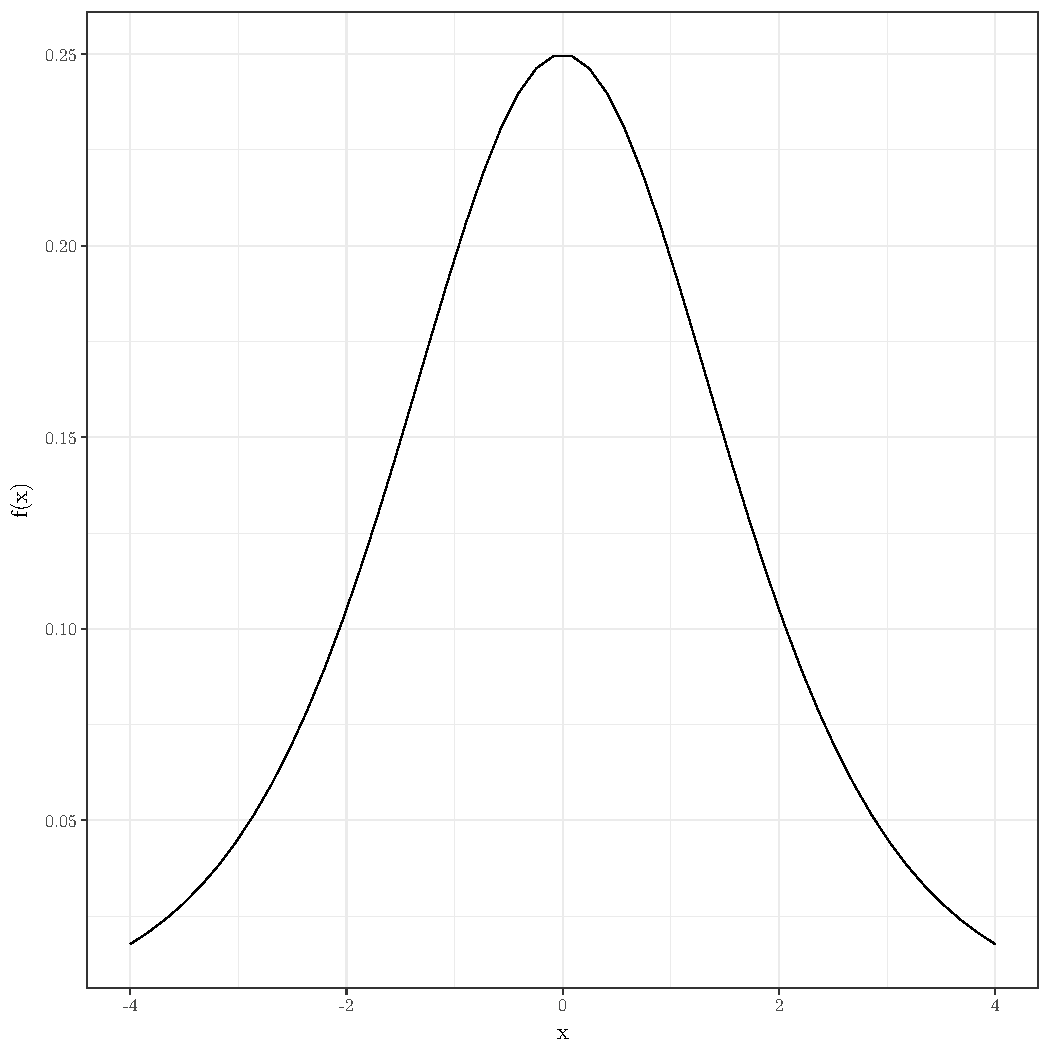
\includegraphics[scale=0.5]{auto_figures_tikz/2014_2015_fig_01_dlogis.pdf}
\end{center}
\end{minipage}
\end{enumerate}


\subsubsection*{Часть 2}

\begin{flushright}
 — Это невозможно! \\
— Нет. Это необходимо.\\
\textcopyright \hspace{0.1cm} Interstellar
\end{flushright}

\begin{enumerate}
\item
Алгоритм решения: рисуешь дерево $\rightarrow$ PROFIT

\begin{center}

 \begin{tikzpicture}[->,>=stealth',shorten >=1pt,auto,node distance=3cm,
  thick,main node/.style={circle,fill=blue!20,draw,font=\sffamily\Large\bfseries}]

  \node[main node] (1) {1};
  \node[main node] (2) [below of=1] {2};
  \node[main node] (3) [below of=2] {3};

  \path[every node/.style={font=\sffamily\small}]
    (1) edge [loop right] node {«не 6»} (1)
        edge [bend right] node[left] {«6»} (2)
    (2) edge [bend right] node[right] {«не 6»} (1)
        edge [above] node[left] {«6»} (3);
\end{tikzpicture}

\end{center}

Комментарии к построению дерева: состояние 1 — начальное, состояние 3 — конец игры,
когда выпало две «шестерки» подряд. Заметим, что выпадение любой «нешестерки» в
процессе игры приводит нас к состоянию, эквивалентному начальному.

Вероятность выпадения «шестерки» равна $1/6$, «нешестерки» — $5/6$.

Теперь мы готовы оседлать коня!

\begin{enumerate}
\item $\P(N = 1) = 0$ — невозможно за ход закончить игру.

$\P(N = 2) = \frac{1}{36}$

$\P(N = 3) = \frac{5}{6} \cdot \frac{1}{6} \cdot \frac{1}{6} = \frac{5}{216}$

\item А теперь будет видна вся сила рисования дерева:

Пусть $\E_1$ — число ходов, за которое мы ожидаем закончить игру, если игра начинается
в состоянии 1, $\E_2$ — число ходов, за которое мы ожидаем закончить игру, если игра
начинается в состоянии 2.

Получим два уравнения:

\[
\begin{cases} \E_2 = \frac{1}{6} \cdot 1 +  \frac{5}{6} (\E_1 + 1)   \\
\E_1 =  \frac{5}{6} (\E_1 + 1) + \frac{1}{6} ( \E_2 + 1) \end{cases}
\]

Решив эту систему, получим, что $\E_1 = 42$. А ведь это и есть $\E(N)$.

Аналогична логика для оставшихся математических ожиданий.

Найдем математическое ожидание суммы набранных очков. Ясно, что если выпадает «не 6»,
то мы ждем 3 очка. Тогда переопределив $\E_1$ и $\E_2$ следующим образом: пусть $\E_1$ —
число набранных очков, которое мы ожидаем получить за игру, если игра начинается
в состоянии 1, $\E_2$ — число набранных очков, которое мы ожидаем получить за игру,
если игра начинается в состоянии 2.

Новые два уравнения:

\[
\begin{cases} \E_2 = \frac{1}{6} \cdot 6 +  \frac{5}{6} (\E_1 + 3)   \\
\E_1 =  \frac{5}{6} (\E_1 + 3) + \frac{1}{6} ( \E_2 + 6) \end{cases}
\]

Решаем и получаем: $\E(S) = \E_1 = 147$

А можно было сделать еще круче! Выше показано, что  $\E(N) = 42$.
А сколько мы ждем очков за 1 ход? 3.5! Тогда $\E(S) = \E(N) \cdot 3.5 = 147$

Применяя схожую логику для $\E\left(N^2\right)$:

\[
\E(N^2) = \frac{5}{6} \cdot \E\left((N + 1)^2\right) + \frac{1}{6} \cdot \frac{5}{6}
\cdot \E\left((N + 2)^2\right) + \frac{1}{6} \cdot \frac{1}{6} \cdot 2^2
\]

Учитывая, что $\E(N) = 42$, получим: $\E(N^2) = 3414$.

\item Veni, vidi, vici
\begin{center}
  \begin{tabular}{@{}cc@{}}
  \toprule
  $x_n$       & $6$ \\
  $\P(X_n = x_n)$ & $1$ \\ \bottomrule
  \end{tabular}
\end{center}
\end{enumerate}

\item
\begin{enumerate}
\item $\P(V = 1) = 1/30$, так как именно этому равна вероятность того, что
Вовочка стоит ровно вторым в очереди;

$M = 1$ значит, что между Машенькой и Вовочкой ровно один человек в очереди.
Если Вовочка находится от 3 (включительно) до 28 позиции в очереди, то для
Машеньки есть две благоприятные позиции для события $M = 1$ (например, если
Вовочка стоит на 15 месте, то благоприятные позиции для Машеньки — стоять либо
13-ой, либо 17-ой). Если же Вовочка стоит на других позициях в очереди, то для
Машеньки существует ровно одна благоприятная позиция:

\[
\P(M = 1) = \frac{26}{30} \cdot \frac{2}{29} +  \frac{4}{30} \cdot \frac{1}{29} = \frac{56}{30\cdot 29} = \frac{28}{435}
\]

$M = V$ произойдет только, если Машенька стоит за Вовочкой. При этом для Машеньки
существует только одна благоприятная позиция и только в том случае, что Вовочка стоит
до 15 позиции (включительно):
\[
\P(M = V) = \frac{1}{2} \cdot \frac{1}{29} = \frac{1}{58}
\]

\item
\[
\E(V) = \frac{0 + 1 + \ldots + 29}{30} = \frac{30\cdot 14 + 15}{30} = 14.5
\]

Для $\E(M)$ можно решить в лоб, и получится красивая сумма, а можно вот так:

Сначала случайно кинем Вовочку и Машеньку на две из 30 позиций в очереди.
Образуется три отрезка: точки между Вовочкой и Машенькой и два крайних отрезка
(может быть, отрезок из 0 точек). Затем будем закидывать в очередь на оставшиеся
позиции случайно 28 оставшихся людей (назовем их «пропавшими»). Т.к. все броски
были случайны (или из соображений симметрии, как хотите), вероятность попасть в
отрезок между Машенькой и Вовочкой для «пропавшего» равна $1/3$, вне отрезка —
соответственно $2/3$, и независима от остальных бросков (!).

Введем случайную величину $X_i$ для $i$-го «пропавшего», которая равна $1$,
если он попал в отрезок между Машенькой и Вовочкой, $0$, если не попал:

\begin{center}
\begin{tabular}{ccc}
\toprule
$x_i$ & $1$ & $0$ \\
$\P(X_i = x_i)$ & $1/3$ & $2/3$ \\ \bottomrule
\end{tabular}
\end{center}

Легко считается: $\E(X_i) = 1/3$, $\E(X^2_i) = 1/3$, $\Var(X_i) = 1/3 - 1/9 = 2/9$.
Ясно, что $M = \sum_1^{28} X_i$. Тогда учитывая независимость $X_i$:

\[
\E(M) = \frac{28}{3}
\]
\[
\Var(M) = \frac{56}{9}
\]
\end{enumerate}

\item
Биномиальное распределение — \textit{À l’abordage!}.

Задача интерпретируется так: последний ход — это когда мы обратились к коробку,
в котором нет спичек (то есть к одному коробку нужно обратиться $n+1$ раз).

\begin{enumerate}
\item Пусть $\xi$ — это случайная величина, обозначающая число оставшихся спичек
в непустом коробке перед последним ходом.

Если $0<k \leqslant n$, будем считать успехом — попадание в коробок, к которому
мы на последнем ходу игры (пустому коробку) обратились. До этого момента из него
было вытащено $n$ спичек, а из другого $n-k$ спичек, то есть спички брались $2n - k$ раз.
Таким образом, перед последним ходом произошло $n$ успехов и $n-k$ неудач.
\[
\P(\xi = k) = C_{2n-k}^{n-k} = \left(\frac{1}{2}\right)^{n-k} \left(\frac{1}{2}\right)^{n} =
C_{2n-k}^{n-k} \left(\frac{1}{2}\right)^{2n-k}
\]
Теперь нужно учесть, что на последнем ходе был выбран именно пустой коробок.
Вероятность этого события — $1/2$, значит, искомая вероятность равна:
\[
\P(\text{в одном коробке осталось k спичек}) = C_{2n-k}^{n-k} \left(\frac{1}{2}\right)^{2n-k}
\cdot \frac{1}{2} = C_{2n-k}^{n-k} \left(\frac{1}{2}\right)^{2n-k+1}
\]
%Успехов — $n + 1$ (вытащено $n$ спичек, и на последнем ходу мы к нему обратились). По формуле Бернулли получаем следующее ($X$ — случайная величина, показывающая сколько спичек осталось в коробке, к которому мы не обратились на последнем ходу игры):
%\[\P(X = k) = C^{n+1}_{2n-k+1} \left(\frac{1}{2} \right)^{2n-k+1}\]

%Если $k = 0$, то мы вытащили все спички из обоих коробков к последнему ходу, и нам без разницы к какому коробку мы обратимся на последнем шагу, т.е.:
%\[\P(X = 0) =2 C^{n+1}_{2n+1} \left(\frac{1}{2} \right)^{2n+1}\]

\item Среднее спичек в другом коробке:

\[
\E(X) = \sum \limits_{k=1}^{n} k \cdot C^{n-k}_{2n-k} \left(\frac{1}{2} \right)^{2n-k+1}
\]

\end{enumerate}

\item
Для того чтобы количество упаковок, которые необходимо купить, равнялось 50,
нужно чтобы ни одну из наклеек Покупатель не встретил дважды, поэтому:
\[
\P(X=50) = 1\cdot\frac{49}{50}\cdot\frac{48}{50}\cdot\dots\cdot\frac{1}{50} =
\frac{49!}{50^{49}} \approx 3.4\cdot
10^{-21}
\] \vspace{-1cm}

\hspace{10.5cm}\fcolorbox{ForestGreen}{white}{Dum spiro, spero!}\footnote[2]{Надежда умирает последней!}

Теперь введём понятие «шаг». Переход на новый шаг происходит в тот момент,
когда покупатель получил наклейку, которой у него раньше не было. Начинаем с шага 0,
когда нет ни одной наклейки, и шагать будем до 49, потому что в момент перехода
на шаг 50 Покупатель получит последнюю необходимую наклейку и «прогулка» закончится.
Введём случайную величину $X_q$ равную количеству покупок в течение шага номер $q$.
Тогда $X = \sum \limits_{q=0}^{49}X_q$.  Найдём математическое ожидание $X_q$:
\[
\E(X_q) = \frac{n-q}{n}\cdot 1 + \frac{q}{n}\cdot\frac{n-q}{n}\cdot 2
+ \left(\frac{q}{n}\right)^2\cdot\frac{n-q}{n}\cdot 3 + \ldots
\]
здесь $\frac{n-q}{n}$ —  это вероятность найти наклейку, которой ещё нет,
а $\frac{q}{n}$, соответственно — вероятность повториться. Вопрос теперь в том,
как посчитать сумму:
\[
\E(X_q) = \frac{n-q}{n}\left( 1 + \frac{q}{n}\cdot 2 + \left(\frac{q}{n}\right)^2 \cdot 3
+ \ldots\right) = \frac{n-q}{n}\cdot\sum\limits_{k=0}^{\infty}\left(\frac{q}{n}\right)^k(k+1)
\]

Можем выписать в столбик несколько первых членов вышестоящей суммы:
\[
\begin{array}{l}
\hspace{0.3cm}1 \\
\vspace{0.2cm}
\left(\frac{q}{n}\right)^1  + \left(\frac{q}{n}\right)^1  \\
\vspace{0.2cm}
\left(\frac{q}{n}\right)^2 + \left(\frac{q}{n}\right)^2  + \left(\frac{q}{n}\right)^2 \\
\left(\frac{q}{n}\right)^3 + \left(\frac{q}{n}\right)^3 + \left(\frac{q}{n}\right)^3 + \left(\frac{q}{n}\right)^3 \\
\hspace{0.1cm}\cdots\cdots\cdots\cdots\cdots\cdots\cdots\cdots\cdots\cdots\cdots
\end{array}
\]
Достаточно! Можем скомпоновать всю сумму другим способом, а именно — по столбцам.
Заметим, что сумма элементов в каждом столбце это сумма бесконечно убывающей
геометрической прогрессии с одним и тем же знаменателем $\frac{q}{n}$ и различными
первыми членами. Соответственно:

\begin{align*}
\sum\limits_{k=0}^{\infty}\left(\frac{q}{n}\right)^k(k+1) &= \frac{1}{1-\frac{q}{n}}
+ \frac{\frac{q}{n}}{1-\frac{q}{n}} + \frac{\left(\frac{q}{n}\right)^2}{1-\frac{q}{n}}
+ \frac{\left(\frac{q}{n}\right)^3}{1-\frac{q}{n}} + \dots = \\
&= \frac{1}{1-\frac{q}{n}}\left( 1 + \frac{q}{n} + \left(\frac{q}{n}\right)^2
+ \left(\frac{q}{n}\right)^3 + \dots\right) = \frac{n}{n-q}\cdot\frac{n}{n-q}
= \left( \frac{n}{n-q}\right)^2
\end{align*}

Таким образом, получаем, что:
\[
\E(X_q) = \frac{n-q}{n}\cdot \left( \frac{n}{n-q}\right)^2 = \frac{n}{n-q}
\]
и это верно для любого q!

\begin{align*}
\E(X) &= \E\left(\sum \limits_{q=0}^{49}X_q\right) = \sum \limits_{q=0}^{49}\E(X_q) =
\frac{50}{50-0} + \frac{50}{50-1} + \dots + \frac{50}{50-49} \\
&= 50\left(\frac{1}{50} + \frac{1}{49} + \dots + 1\right)
\approx 50\int\limits_{1}^{50}\frac{1}{x}\mathbf{d}x = 50\ln(50) \approx 195.5
\end{align*}

А теперь ещё одно решение:


Величины $X_q$ независимы (но по разному распределены). Если долго пришлось ждать
$i$-го шага, это ничего не говорит о $j$-ом шаге. Величины $X_q$ имеют известный
закон распределения — это число опытов до первого успеха при заданной вероятности
успеха. Это геометрическое распределение, математическое ожидание которого равно
$\frac{1}{p}$, а дисперсия: $\frac{1-p}{p^2}$, где $p$ — \vspace{0.2cm} вероятность
успеха.

А те, кто забыл, могут \textbf{проще решить} методом первого шага:
если $X$ — число опытов до успеха при вероятности успеха $p$, то
\[
\E(X)=p\cdot 1 + (1-p)\cdot \E(X+1)
\]
Откуда $\E(X) = 1/p$ и дело в шляпе :)
Аналогично:
\[
\E(X^2)=p\cdot 1^2 + (1-p) \cdot \E((X+1)^2)
\]
и решая, находим $\E(X^2)$.

\item
\begin{enumerate}
\item Необходимое и достаточное условие — старушка не должна занять чужое место.
С вероятностью $1/n$ она угадает свое место, значит, для каждого входящего
его место будет свободно и он туда сядет.

\textbf{Ответ:} $1/n$
\item Будем искать вероятность того, что последний человек не сядет на свое место.

Пусть $A_i = \{\text{Старушка села на  место } i\text{-го} \}$,
$B_{(i,j)} = \{i \text{-ый  пассажир сел на место } j\text{-ого} \}$

\begin{align*}
P(n\text{-ый не сядет на свое место}) &= \P(A_n) + P(A_{n-1})P(B_{(n-1,n)}) + \\
&+ P(A_{n-2})(P(B_{(n-2,n)})
+ P(B_{(n-2,n-1)})P(B_{(n-1,n)}))) + \dots
\end{align*}

Можем заметить, что:
\begin{itemize}
\item $\P(A_i) = P(A_j) = \frac{1}{n}$ $\forall \hspace{0.1cm} i, j$
\item $\P(B_{(n-1,n)}) = \frac{1}{2}$, потому что $n-1$-ый выбирает из двух оставшихся мест
\item $\P(B_{(n-2,n)})
+ \P(B_{(n-2,n-1)}]P[B_{(n-1,n)})  = \frac{1}{3} + \frac{1}{3}\cdot \frac{1}{2} = \frac{1}{2}$
\item
\begin{align*}
\P(B_{(n-3,n)}) &+ \P(B_{(n-3,n-2)})(\P(B_{(n-2,n)})+\P(B_{(n-2,n-1)})\P(B_{(n-1,n)})) \\
&+ \P(B_{(n-3,n-1)})\P(B_{(n-1,n)}) = \frac{1}{4}+\frac{1}{4}\left(\frac{1}{3}+\frac{1}{3}\cdot\frac{1}{2}\right) +\frac{1}{4}\cdot \frac{1}{2} = \frac{1}{2}
\end{align*}
\item И так далее до того момента, пока старушка не сядет на место первого человека,
который заходит после нее, — всего $n-2$ вариантов.
\end{itemize}

Таким образом мы получаем сумму:
\[
\P[n\text{-ый не сядет на свое место}] = \frac{1}{n} + \frac{1}{n}\cdot \frac{1}{2}
+ \frac{1}{n}\cdot \frac{1}{2} + \dots = \frac{1}{n}  + \frac{1}{2n}(n-2) = \frac{1}{2}
\]
Значит,
\[
\P[n\text{-ый сядет на свое место}] = 1 - \frac{1}{2} = \frac{1}{2}
\]


А вот ещё один вариант решения:

\underline{Метод математической индукции:} допустим что это утверждение доказано
для одного, двух и так далее до $k$ человек. Рассмотрим $k+1$ человека. Когда
последний сядет на своё место? Если старушка сядет на своё место, а вероятность
этого равна $\frac{1}{k+1}$ или, с вероятностью $\frac{1}{2}$ (по индукции),
если старушка сядет на любое место кроме своего и последнего, то есть
$\frac{1}{2}\cdot\frac{k-1}{k+1}$. В этом случае тот\vspace{0.2cm} пассажир,
чьё место  она заняла, становится старушкой, и мы получаем задачу при меньшем $k$.
Складывая эти две дроби, получаем $\frac{1}{2} $.

Чтобы найти среднее число пассажиров, разобьем эту величину в сумму индикаторов:
$Y_1$ — сел ли первый на место, $\dots$, $Y_n$ — сел ли $n$-ый на место
(индикатор равен единице, если сел).

Стало быть $\E(Y)=\E(Y_1)+\E(Y_2)+\ldots+\E(Y_n)$. $\E(Y_n)=\frac{1}{2}$.

Почти аналогично можем рассуждать для предпоследнего:

База индукции: если пассажиров трое ($n=3$ включая старушку), то для предпоследнего
вероятность сесть на своё место равна $\frac{2}{3}$.

Шаг индукции: допустим что для $3, 4, \ldots n$ пассажиров эта вероятность равна
$\frac{2}{3}$.
Рассмотрим случай $(n+1)$-го пассажира.
Предпоследний сядет на своё место, если:

\renewcommand{\labelitemi}{\textbullet}

\begin{itemize}
\item старушка сядет на своё место или на место последнего $\frac{2}{n+1}$
\item в $\frac{2}{3}$ тех случаев, когда старушка сядет на место $2, 3, \ldots, (n-1)$,
то есть $\frac{2}{3}\cdot \frac{n-2}{n+1}$ складываем, получаем $\frac{2}{3}$.
То есть по индукции вероятность того, что предпоследний сядет на своё место равна
$\frac{2}{3}$.
\end{itemize}
И по аналогии можно увидеть, что вероятность того, что $k$-ый с конца пассажир
сядет на своё место равна $k/(k+1)$.

Если у нас $n$ пассажиров включая СС, то среднее количество севших на свои места
(раскладывая с конца) равно
\[
\frac{1}{2}+\frac{2}{3}+\frac{3}{4}+\dots+\frac{n-1}{n}+\frac{1}{n}
\]
\end{enumerate}
\end{enumerate}



\subsection[2013-2014]{\hyperref[sec:kr_01_ip_2013_2014]{2013-2014}}
\label{sec:sol_kr_01_ip_2013_2014}


\subsubsection*{Часть 1}

\begin{enumerate}
\item
\begin{enumerate}
\item Запишем все благоприятные исходы в таблицу:

\begin{center}
\begin{tabular}{@{}ll@{}}
\toprule
Исход & Вероятность             \\ \midrule
ООО   & $p^2 \cdot \frac{1}{2}$ \\
ООН   & $p^2 \cdot \frac{1}{2}$ \\
ОНО   & $ p(1-p)\frac{1}{2}$    \\
НОО   & $ (1-p)p\frac{1}{2}$    \\ \bottomrule
\end{tabular}
\end{center}

Нас устраивает любой из этих исходов, так что
\[
\P(\text{жюри одобрит конкурсанта}) = p^2 \cdot \frac{1}{2} \cdot 2 +
p(1-p)\frac{1}{2} \cdot 2 = p
\]
\item Исходя из результата предыдущего пункта, получаем, что конкурсанту безразлично.
\end{enumerate}

\item Введём обозначения:
\begin{itemize}
\item $\P(\text{В} | \text{A}^{c} \cap \text{М}^{c}) = p$ — Вася пришёл, а девушки — нет.
\item $\P(\text{В} | \text{A} \cap \text{М}) = 5p$ — пришли и Вася, и девушки.
\item $\P(\text{В} | \text{A}^{c} \cap \text{М}) = 3p$ — Вася пришёл, если пришла только Маша.
\item $\P(\text{В} | \text{A} \cap \text{М}^{c}) = 2p$ — Вася пришёл, если пришла только Алёна.
\item $\P(\text{М}) = 0.6$ — Маша пришла на лекцию.
\item $\P(\text{А}) = 0.3$ — Алёна пришла на лекцию.
\end{itemize}
\begin{enumerate}
\item По теореме умножения:
\[
\P(\text{А} | \text{В}) = \frac{\P(\text{А} \cap \text{В})}{\P(\text{В})}
\]
Выпишем числитель:
\begin{align*}
\P(\text{В} | \text{A}) \cdot \P(\text{А}) &= P(\text{В} | \text{A} \cap \text{М}) \cdot \P(\text{А}) \cdot \P(\text{М}) + \P(\text{В} | \text{A} \cap \text{М}^{c}) \cdot \P(\text{А}) = \cdot \P(\text{М}^{c}) \\
&= 5p \cdot  0.6 \cdot 0.3 \cdot 0.6 + 2p \cdot 0.36 \cdot 0.4 \cdot 0.3 = 1.14p
\end{align*}
И знаменатель:
\begin{align*}
\P(\text{В} | \text{A}^{c} \cap \text{М}^{c}) \cdot \P(\text{A}^{c} \cap \text{М}^{c}) &+ \P(\text{В} | \text{A} \cap \text{М}) \cdot \P(\text{A} \cap \text{М}) + \P(\text{В} | \text{A}^{c} \cap \text{М}) \cdot \P(\text{A}^{c} \cap \text{М})+ \\
&+  \P(\text{В} | \text{A} \cap \text{М}^{c}) \cdot \P(\text{A} \cap \text{М}^{c}) = p \cdot 0.4 \cdot 0.7 + 5p \cdot 0.6 \cdot 0.3 \\
&+ 3p \cdot 0.6 \cdot 0.7 + 2p \cdot 0.4 \cdot 0.3 = 2.68p
\end{align*}
Ответ:
\[
\P(\text{A} | \text{В} ) = \frac{\P(\text{A} \cap \text{В})}{\P(\text{В})} = \frac{1.14 p}{2.68p}  \approx 0.43
\]
\item Теперь необходимо найти
\[
\P(\text{М} | \text{В}) = \frac{\P(\text{М} \cap \text{В})}{\P(\text{В})}
\]
Знаменатель этой дроби посчитан в предыдущем пункте, посчитаем числитель:
\begin{align*}
\P(\text{М} \cap \text{В}) &= \P(\text{В} | \text{М}) \cdot \P(\text{М}) = P(\text{В} | \text{М} \cap \text{А}) \cdot \P(\text{А}) \cdot \P(\text{М}) \\
&+ \P(\text{В} | \text{A}^{c} \cap \text{М}) \cdot \P(\text{А}^{c})  \cdot \P(\text{М}) = 5p \cdot 0.6 \cdot 0.3 + 3p \cdot 0.6 \cdot 0.7 = 2.16p
\end{align*}
Ответ:
\[
\P(\text{М} | \text{В}) = \frac{\P(\text{М} \cap \text{В})}{\P(\text{В})} = \frac{2.16p}{2.68p} \approx 0.8
\]
Если Вася на лекции, вероятность застать на ней Машу выше.
\item $\P(\text{В}) = 0.5$, $ \P(\text{В}) = 2.68 p \Rightarrow p \approx 0.19$
\end{enumerate}
\item
\begin{enumerate}
\item Перед нами биномиальное распределение! Пусть $X$ — случайная величина, число туристов, которые не выехали за границу. Тогда:
\[
\P(X=5) = C_{100}^{5} \cdot 0.002^{5} \cdot 0.998^{95}
\]
\item
\begin{itemize}
\item $\E(X) = 2$
\item $\Var(X) = 0.2 \cdot 0.998$
\item Наиболее вероятное число невыехавших — 0.
\end{itemize}
\item Пусть случайная величина $S_i$ обозначает страховые выплаты, которые может
получить один турист. Она может принимать значение $0$, если турист выехал за границу
и не обратился за медицинской помощью, $ 2000$, когда он не выехал и $3000$,
когда турист выехал за границу и обратился за медицинской помощью. Тогда $S_i$
распределена следующим образом:
\begin{center}
\begin{tabular}{@{}lccc@{}}
\toprule
$s_i$       & $0$                & $2000$  & $3000$             \\ \midrule
$\P(S_i = s_i)$ & $0.998 \cdot 0.99$ & $0.002$ & $0.998 \cdot 0.01$ \\ \bottomrule
\end{tabular}
\end{center}
\begin{itemize}
\item $\E(S_i) = 2000 \cdot 0.002 + 3000 \cdot 0.998 \cdot 0.01 = 33.94 \Rightarrow \E(S) = 3394$
\item $\E(S_i^2) = 2000^2 \cdot 0.002 + 3000^2 \cdot 0.998 \cdot 0.01 = 97820 $
\item $\Var(S_i) = 97820 - 33.94^2 = 96668 \Rightarrow \Var(S) = 9666800$
\end{itemize}
\item
\end{enumerate}
\item
\begin{enumerate}
\item $\E(Y - 2X - 3) = \E(Y) - 2 \E(X) - 3 = 0$

$\Var(Y - 2X - 3) = \Var(Y) + 4\Var(X) - 2\Cov(Y, 2X) = 16$

$\Cov(X, Y) = \Corr(X,Y) \cdot \sqrt{\Var(X) \cdot \Var(Y)} = 6$
\item $\Corr(Y - 2X - 3, X) = \frac{\Cov(Y, X) - 2 \Var(X)}{\sqrt{\Var(Y - 2X - 3) \cdot \Var(X)}} = -1$, или проще: можно было заметить, что случайные величины линейно связаны.
\item Корреляция равна 1, значит, есть линейная взаимосвязь между переменными. Пусть $Y+ a X = b$, тогда $\Var(Y+ a X)=0$, $\E(Y) = -a + b =1 $. Решая уравнения, находим, что $a=-2/3, b=1/3$.
\end{enumerate}
\item
\begin{enumerate}
\item Частные распределения:

\begin{tabular}{@{}lccl@{}}
\toprule
$x$         & $-1$  & $0$   & $1$   \\ \midrule
$\P(X=x)$ & $0.3$ & $0.3$ & $0.4$ \\ \bottomrule
\end{tabular}
\hspace{1cm}
\begin{tabular}{@{}lcc@{}}
\toprule
$y$         & $-1$  & $1$   \\ \midrule
$\P(Y=y)$ & $0.5$ & $0.5$ \\ \bottomrule
\end{tabular}
\item
\begin{align*}
\Cov(X, Y) &= \E(XY) - \E(X)\E(Y) = (-1) \cdot (-1) \cdot 0.1 + (-1) \cdot 1 \cdot 0.2 + 1 \cdot (-1 ) \cdot 0.2 \\
 &+ 1 \cdot 1 \cdot 0.2 - ((-1) \cdot 0.3 + 1 \cdot 0.4) (-1\cdot 0.5 + 1 \cdot 0.5) = -0.1
\end{align*}
\item Да, так как $\Cov(X, Y) \neq 0$
\item Необходимо минимизировать дисперсию дохода:
\[\Var(\alpha X + (1- \alpha)Y) \to \min_{\alpha} \]
\begin{align*}
\Var(\alpha X + (1 - \alpha)Y)  &= \alpha^2 \Var(X) + (1 - \alpha)^2 \Var(Y) + 2 \alpha(1 - \alpha)\Cov(X, Y) \\
&= 0.69 \alpha^2  + (1 - \alpha)^2 -0.2 \alpha(1 - \alpha) \to \min_{\alpha}
\end{align*}
\[
\frac{\partial \Var(\alpha X + (1- \alpha)Y)}{\partial \alpha} = 2 \cdot 0.69 \alpha - 2(1-\alpha) -0.2 + 0.4 \alpha = 0 \Rightarrow
\alpha \approx 0.58
\]
\item Условное распределение:

\begin{center}
\begin{tabular}{@{}lclc@{}}
\toprule
$x$ & $-1$  & $0$   & $1$   \\ \midrule
$\P(X = x\mid Y=-1)$    & $0.2$ & $0.4$ & $0.4$ \\ \bottomrule
\end{tabular}
\end{center}

\item $\E(X \mid Y=-1) = -1 \cdot 0.2 + 1 \cdot 0.4 = 0.2$
\end{enumerate}
\end{enumerate}

\section{Решения контрольной номер 2}

\subsection[2017-2018]{\hyperref[sec:kr_02_2017_2018]{2017-2018}}
\label{sec:sol_kr_02_2017_2018}

\begin{enumerate}
\item[7.]
\begin{enumerate}
\item Всем хватит места, если число явившихся на рейс пассажиров ($X$) не превысит $300$,
то есть нужно найти $\P(X \leq 300)$. Найдём матожидание и дисперсию
случайной величины $X$:
\begin{align*}
\E(X) &= np = 330 \cdot 0.9 = 297 \\
\Var(X) &= np(1-p) = 330 \cdot 0.9 \cdot 0.1 = 29.7
\end{align*}
Теперь посчитаем нужную вероятность:
\[
\P(X \leq 300) = \P \left(\frac{X - 297}{\sqrt{29.7}} \leq \frac{300 - 297}{\sqrt{29.7}} \right) = \P(\cN(0,1) \leq 0.55) \approx 0.709
\]
\item Вероятность переполнения не должна превышать $0.1$:
\begin{align*}
&\P(X > 300) < 0.1 \\
&\P\left(\frac{X - 0.9 \cdot n}{\sqrt{0.9 \cdot 0.1 \cdot n}} > \frac{300 - 0.9 \cdot n}{\sqrt{0.9 \cdot 0.1 \cdot n}} \right) < 0.1 \\
&\frac{300 - 0.9 \cdot n}{\sqrt{0.9 \cdot 0.1 \cdot n}}  > 1.28 \\
&300 - 0.9n > 1.28 \cdot 0.3 \sqrt{n} \\
&n < 325.6
\end{align*}
\end{enumerate}
\item[8.]
\begin{enumerate}
\item Выпишем случайную величину $X_i$ — цену акции после $i$-ого дня:
\[
X_i =
\begin{cases}
1.01, & p = 0.7 \\
0.99, & p = 0.2999 \\
0, & p = 0.0001
\end{cases}
\]
Нужно посчитать ожидание цены акциии после 20 дней:
\[
\E(X_1 \cdot \ldots \cdot X_{20}) \stackrel{\text{незав-ть}}{=} \E(X_1) \cdot \ldots \cdot \E(X_{20}) = 1.004^{20} \approx 1.083
\]
\item По ЗБЧ:
\[
\plim_{n\to\infty} \frac{1}{n} \sum_{i=1}^n X_i = \E(X_i) = 1.004
\]
\item Аналогично пункту (а):
\[
\E(X_1 \cdot \ldots \cdot X_{n}) = (\E(X_1))^n = 1.004^n
\]
И понятно, что $1.004^n \to_{n\to\infty} +\infty$.
\item
\begin{multline*}
\P(\text{разорения}) = 1 - \P(X_1 > 0, \ldots, X_n >0) = 1 - \prod_{i=1}^n \P(X_i > 0) \\
= 1 - (1 - 0.0001)^n \to_{n\to\infty} 1
\end{multline*}
\end{enumerate}
\end{enumerate}



\subsection[2016-2017]{\hyperref[sec:kr_02_2016_2017]{2016-2017}}
\label{sec:sol_kr_02_2016_2017}



\begin{enumerate}
\item \begin{enumerate}
\item $\E (2\xi - \eta +1) = 2 \E (\xi) - \E (\eta) + 1 = 2\cdot 1 - (-2) + 1 = 5 $

$\Cov (\xi, \eta) = \E (\xi \eta) - \E(\xi) \E(\eta) = -1 - \cdot 1 \cdot (-2) = 1$

$\Corr (\xi, \eta) = \frac{\Cov(\xi, \eta)}{\sqrt[]{\Var(X) \cdot \Var(Y)}} = \frac{1}{\sqrt{1 \cdot (8-(-2)^2)}} = \frac{1}{2}$

$\Var (2\xi - \eta + 1) = 4\Var(\xi) + \Var(\eta) - 2 \Cov (2\xi, \eta) = 4 \cdot 1 + 4 - 4 \cdot 1 = 4$

\item $\Cov(\xi + \eta, \xi + 1) = \Cov(\xi) + \Cov(\xi, 1) + \Cov(\eta, \xi) + \Cov(\eta, 1) = 1 +1 = 2$

$\Corr(\xi + \eta , \xi + 1) = \frac{\Cov(\xi + \eta , \xi + 1)}{\sqrt{\Var(\xi + \eta)\cdot \Var (\xi + 1)}} = \frac{2}{\sqrt{(1+4+2\cdot 1) \cdot 1}} = \frac{2}{\sqrt{7}}$

$\Corr(\xi + \eta - 24, 365 - \xi - \eta) = -1$

$\Cov(2016\cdot \xi, 2017) = 0$

\end{enumerate}
\item \begin{enumerate}
\item
\begin{center}
\begin{tabular}{cccc}
\toprule
$\xi$ & $-1$ & $0$ & $2$ \\ \midrule
$\P(\cdot)$ & $0.3$ & $0.4$ & $0.3$ \\ \bottomrule
\end{tabular}
\hspace{1cm}
\begin{tabular}{ccc}
\toprule
$\eta$ & $-1$ & $1$ \\ \midrule
$\P(\cdot)$ & $0.5$ & $0.5$ \\ \bottomrule
\end{tabular}
\end{center}

$\E(\xi) = -1 \cdot 0.3 + 0 \cdot 0.4 + 2 \cdot 0.3 = 0.3$

$\E (\xi^2) = (-1)^2 \cdot 0.3 + 0^2 \cdot 0.4 + 2^2 \cdot 0.3 = 1.5$

$\Var(\xi) = \E(\xi^2) - (\E(\xi))^2 = 1.5 - 0.3^2 = 1.41$

$\E(\eta) = -1 \cdot 0.5 + 1 \cdot 0.5 = 0$

$\E(\eta^2) = (-1)^2 \cdot 0.5 + 1^2 \cdot 0.5 = 1$

$\Var(\eta) = \E(\eta^2)-(\E(\eta))^2 = 1 - 0^2 = 1$

\item
\begin{center}
\begin{tabular}{cccccc}
\toprule
$\xi \cdot \eta$ & $-2$ & $-1$ & $0$ & $1$ & $2$ \\ \midrule
$\P(\cdot)$ & $0.2$ & $0.2$ & $0.4$ & $0.1$ & $0.1$ \\ \bottomrule
\end{tabular}
\end{center}

$\E(\xi\cdot\eta) = (-2) \cdot 0.2 + (-1) \cdot 0.2 + 0 \cdot 0.4 + 1\cdot 0.1 + 2 \cdot 0.1 = -0.3$

$\Cov(\xi, \eta) = \E(\xi\cdot\eta) - \E(\xi)\cdot\E(\eta) = -0.3 - 0.3 \cdot 0 = -0.3$
\item Пусть случайная величина $X$ принимает значения $a_1, \ldots, a_m$, случайная веилчина $Y$ принимает значения $b_1, \ldots, b_n$. Тогда случйаня величина $X$ и $Y$ называются независимыми, если $\forall i=1, \ldots, m \quad \forall j=1, \ldots, n: \P(X = a_i \cap Y = b_j) = P(X = a_i) \cdot P(Y = b_j)$
\item Заметим, что $\P (\xi = -1 \cap \eta=-1)=0.1$, $\P(\xi=-1)=0.3$ и $\P(\eta=-1)=0.5$.

Тогда поскольку $\P (\xi = -1 \cap \eta=-1) \neq \P(\xi=-1) \cdot \P(\eta=-1)$, случайные величины $\xi$ и $\eta$ не являются независимыми.
\item $\P (\xi = -1 \cap \eta=1) = \frac{\P (\xi = -1 \cap \eta=1)}{\P(\eta=1)} = \frac{0.2}{0.5} = \frac{2}{5}$

$\P (\xi = 0 \cap \eta=1) = \frac{\P (\xi = 0 \cap \eta=1)}{\P(\eta=1)} = \frac{0.2}{0.5} = \frac{2}{5}$

$\P (\xi = 2 \cap \eta=1) = \frac{\P (\xi = 2 \cap \eta=1)}{\P(\eta=1)} = \frac{0.1}{0.5} = \frac{1}{5}$

Следовательно, условное распределение случайной величины $\xi$ при условии $\{\eta=1\}$ может быть описано следующей таблицей:

\begin{center}
\begin{tabular}{cccc}
\toprule
$\xi$ & $-1$ & $0$ & $2$ \\ \midrule
$\P(\cdot)$ & $2/5$ & $2/5$ & $1/5$ \\ \bottomrule
\end{tabular}
\end{center}

\item $\E(\xi \mid \eta = 1) = -1 \cdot \frac{2}{5} + 0 \cdot \frac{2}{5} + 2 \cdot \frac{1}{5} = 0$
\item $\E(\pi) = \E(0.5 \xi + 0.5 \eta) = 0.5 \E(\xi) + 0.5 \E(\eta) = 0.15$

\begin{align*}
\Var(\pi) &= \Var(0.5 \xi + 0.5 \eta) = \Var(0.5 \xi) + \Var(0.5\eta) + 2 \Cov (0.5\xi, 0.5\eta) \\
&= 0.25\Var(\xi) + 0.25\Var(\eta) + 2 \cdot 0.5 \cdot 0.5 \Cov(\xi, \eta) \\
&= 0.25 \cdot 1.41 + 0.25 \cdot 1 + 2 \cdot 0.5 \cdot 0.5 \cdot (-0.3) = 0.4525
\end{align*}
\item
\begin{align*}
\Var(\pi(\alpha)) &= \Var(\alpha \xi + (1-\alpha)\eta) = \alpha^2\Var(\xi) + (1-\alpha)^2 \Var(\eta) \\
&+ 2\alpha(1-\alpha) \Cov(\xi, \eta) = 1.41 \cdot \alpha^2 + 1\cdot (1-\alpha)^2 + 2\alpha(1-\alpha) \cdot (-0.3) \\
&= 1.41 \cdot \alpha^2 + (1-\alpha)^2 - 0.6 \cdot (\alpha - \alpha^2) \to \min_\alpha \\
\frac{\partial}{\partial \alpha} \Var(\pi(\alpha)) &= 2 \cdot 1.41 \cdot \alpha -2(1-\alpha) -0.6\cdot(1-2\alpha) \\
&= 2.82 \cdot \alpha - 2 + 2\alpha - 0.6 + 1.2 \cdot \alpha = 6.02 \cdot \alpha - 2.6 = 0 \\
\alpha &= \frac{2.6}{6.02} = 0.4319
\end{align*}
\end{enumerate}
\item \begin{enumerate}
\item Для любой неотрицательной случайной величины $X$ и любого числа $\lambda > 0$ справедлива оценка: $\P(X>\lambda) \leq \frac{\E(X)}{\lambda}$

Пусть случайная величина $\xi_i$ означает число посетителей сайта за $i$-ый день. По условию, $\xi_i \sim Pois(\lambda=250)$. Известно, что если $\xi \sim Pois(\lambda)$, то $\E(\xi) = \Var(\xi) = \lambda$.

Имеем:
\[
\P(\xi_i >500) \leq \P(\xi_i \geq 500) \leq \frac{\E(\xi_i)}{500} = \frac{250}{500} = \frac{1}{2}
\]
\item Для любой случайной величины $X$ с конечным $\E(X)$ и любого положительного числа $\epsilon > 0$ имеет место неравенство: $\P(X-\E(X)\geq\epsilon)\leq\frac{\Var(X)}{\epsilon^2}$

Обозначим $\bar{\xi}_n := \frac{1}{n} \left(\xi_1 + \ldots + \xi_n\right)$ – среднее число посетителей сайта за $n$ дней. Тогда
\[
\E(\bar{\xi}_n) = \E\left(\frac{1}{n} \sum_{i=1}^{n} \xi_i\right) = \frac{1}{n} \sum_{i=1}^{n} \E(\xi_i) = \frac{1}{n} \cdot n \cdot \lambda = \lambda = 250
\]
\[
\Var(\bar{\xi}_n) = \Var\left(\frac{1}{n} \sum_{i=1}^{n} \xi_i\right) = \frac{1}{n^2} \sum_{i=1}^{n} \Var (\xi_i) = \frac{n \cdot \lambda}{n^2} = \frac{\lambda}{n} = \frac{250}{n}
\]
Оценим вероятность
\[
\P(\vert\bar{\xi}_n-250\vert > 10) \leq \frac{\Var(\bar{\xi}_n)}{100} = \frac{250}{100\cdot n}
\]
Следовательно, $1 - \frac{250}{100\cdot n} \leq \P(\vert\bar{\xi}_n-250\vert \leq 10)$.

Найдём наименьшее целое $n$, при котором левая часть неравенства ограничена снизу $0.99 \leq 1 - \frac{250}{100\cdot n}$.

Имеем:
\[
0.99 \leq 1 - \frac{250}{100\cdot n} \Leftrightarrow \frac{250}{100\cdot n} \leq 0.01 \Leftrightarrow n \geq \frac{250}{100 \cdot 0.01} \Leftrightarrow n  \geq 250
\]
Значит, $n=250$ – наименьшее число дней, при котором с вероятностью не менее $99\%$ среднее число посетителей будет отличаться от $250$ не более чем на $10$.
\item  Требуется найти наименьшее целое $n$, при котором $\P(\vert\bar{\xi}_n-250\vert \leq 10)=0.99$

Имеем:
\begin{multline*}
\P(\vert\bar{\xi}_n-250\vert \leq 10)=0.99 \Leftrightarrow \P(-10\leq \bar{\xi}_n -250 \leq 10) =0.99 \Leftrightarrow \\
\Leftrightarrow  \P(-10n \leq S_n-250n \leq 10n) =0.99
\end{multline*}
\[
\E(S_n) = \E(\xi_1 + \ldots + \xi_n) = \E(\xi_1) + \ldots + \E(\xi_n) = 250\cdot n
\]
\[
\Var(S_n) = \Var(\xi_1 + \ldots + \xi_n) = \Var(\xi_1) + \ldots + \Var(\xi_n) = 250 \cdot n
\]
\begin{multline*}
\P\left(\frac{-10n}{\sqrt{250n}} \leq \frac{S_n - \E (S_n)}{\sqrt{\Var(S_n)}} \leq \frac{10n}{\sqrt{250n}}\right) =0.99 \Leftrightarrow 2 \Phi \left(\frac{10n}{\sqrt{250n}}\right) -1 = 0.99 \\
\Phi \left(\frac{10n}{\sqrt{250n}}\right) = \frac{1 + 0.99}{2} \Leftrightarrow \frac{10n}{\sqrt{250n}} = 2.58 \Leftrightarrow \sqrt{n} = 2.58 \cdot \frac{\sqrt{250}}{10} \Leftrightarrow n = 16.641
\end{multline*}
Следовательно, наименьшее целое $n$, есть $n=17$.
\item Пусть $X_1, X_2, \ldots, X_n, \ldots$ – последовательность независимых случайных величин с одинаковыми конечными математическими ожиданимяи и фиксированными конечными дисперсиями. Тогда $\frac{X_1 + \ldots + X_n}{n} \stackrel{\P}{\to} \E(X_i)$ при $n \to \infty$.

В нашем случае случаные величины $\xi_1^2, \xi_2^2, \ldots, \xi_n^2, \ldots$ – независимы,

$\E(\xi_1^2) = \ldots = \E(\xi_n^2) = \ldots < + \infty$ и $\Var(\xi_1^2) = \ldots = \Var(\xi_n^2) = \ldots < + \infty$ . Поэтому в соответствии с ЗБЧ имеем:
\[
\frac{\xi_1^2 +\ldots+ \xi_n^2}{n} \stackrel{\P}{\to} \E(\xi_i^2) = \Var(\xi_i) +\E(\xi_i)^2 = \lambda + \lambda^2 = \lambda(\lambda+1) = 250\cdot251 = 62750
\]
\end{enumerate}

\item \begin{enumerate}
\item Пусть $X_1, X_2, \ldots, X_n, \ldots$ – последовательность независимых, одинаково распределённых случайных величин с $0<\Var(X_i)<\infty$, $i \in \mathbb{N}$.  Тогда для любого (борелевского) множества $B \subseteq R$ имеет место $\lim_{n \to \infty} \P\left(\frac{S_n - \E(S_n)}{\sqrt{\Var(S_n)}} \in B\right) = \int_B \frac{1}{\sqrt{2\pi}}e^{-t^2/2} dt$, где $S_n := X_1, \ldots, X_n$, $n \in \mathbb{N}$.
\item Введём случайную величину
\[
X_i = \begin{cases}
1, & \text{если на i-ом шаге Винни-Пух пошёл направо} \\
-1, & \text{если пошёл налево}
\end{cases}
\quad i=1,\ldots, n;
\]
Тогда $S_n := X_1 +\ldots+X_n$ означает местоположение Винни-Пуха в $n$-ую минуту его блужданий по прямой.

$\E(X_i) = -1 \cdot 1/2 + 1 \cdot 1/2 = 0$,

$\E(X_i^2) = (-1)^2 \cdot 1/2 + (1)^2 \cdot 1/2 = 1$,

$\Var(X_i) = \E(X_i^2) - \E(X_i)^2 = 1$,

$\E(S_n) = \E(X_1 + \ldots + X_n ) = \E(X_1) + \ldots + \E(X_n) = 0$,

$\Var(S_n) = \Var(X_1 + \ldots + X_n ) = \Var(X_1) + \ldots + \Var(X_n) = n$

\begin{multline*}
\P(S_n \in (-\infty, -5]) = \P(S_n \leq -5) = \P\left( \frac{S_n-\E(S_n)}{\sqrt{\Var(S_n)}} \leq \frac{-5-0}{\sqrt{n}} \right) \stackrel{n=60}{=} \\
=\P\left( \frac{S_n-\E(S_n)}{\sqrt{\Var(S_n)}} \leq -0.6454\right) \approx \int_{-\infty}^{-0.6454} \frac{1}{\sqrt{2\pi}} e^{-t^2/2} dt = \\
= \Phi(-0.6454) = 1-\Phi(0.6454) \approx0.2593
\end{multline*}
\item Для любых $n \in \mathbb{N}$ и всех $x \in \mathbb{R}$ имеет место оценка:
\[
\bigl|F_{S_n^{*}}(x) - \Phi(x)\bigr| \leq 0.48 \cdot \frac{\E(|\xi_i - \E\xi_i|^3)}{\Var^{3/2}(\xi_i)\cdot\sqrt{n}} \text{,}
\]
где $\Phi(x) = \int_{-\infty}^{x}\frac{1}{\sqrt{2\pi}}e^{-\frac{t^2}{2}}\,dt$, \; $S_n^* = \frac{S_n - \E(S_n)}{\sqrt{\Var(S_n)}}$, \; $S_n = \xi_1 + \ldots + \xi_n$

В нашем случае:
\[
\P\left( \frac{S_{60} - \E(S_{60})}{\sqrt{\Var(S_{60})}} \leq -0.6454 \right) = \P(S^*_{60} \leq -0.6454) =
F_{S^*_{60}} (-0.6454)
\]
Согласно неравенству Берри-Эссеена, погрешность $\vert F_{S^*_{60}} (-0.6454) - \Phi(-0.6454) \vert$ оценивается сверху величиной
\[
0.48 \cdot \frac{\E(\vert X_i - \E(X_i) \vert^3 )}{\Var(X_i)^{3/2} \cdot \sqrt{n}} = 0.48 \cdot \frac{\E(\vert X_i \vert^3)}{1\cdot\sqrt{60}} = \frac{0.48}{\sqrt{60}} \approx0.062
\]
\end{enumerate}
\item \begin{enumerate}
\item Сначала найдём плотность распределения случайной величины $X$. Пусть $x \leq 0 $, тогда $f_X (X) = \int_{-\infty}^{+\infty} f_{X, Y} (x, y) dy  = 0$;

Пусть $x >0 $, тогда
\begin{multline*}
f_X (X) = \int_{-\infty}^{+\infty} f_{X, Y} (x, y) dy = \int_{0}^{+\infty} 0.005 e^{-0.05x-0.1y} dy = \\
= 0.005e^{-0.05x} \int_{0}^{+\infty} e^{-0.1y} dy = 0.005e^{-0.05x} \cdot \left(-10e^{-0.1y} \right) \bigg\vert_{y=0}^{y=+\infty} = 0.05 e^{-0.05x}
\end{multline*}
Таким образом, имеем:
\[
f_X (x) = \begin{cases}
0.05 e^{-0.05x} & \text{при } x>0 \\
0 & \text{при } x \leq 0
\end{cases}
\]
То есть $X \sim Exp(\lambda=0.05)$ – случайная величина $X$ имеет показательное распределение с параметром $\lambda = 0.05$.

Теперь найдём плотность распределения случайной величины $Y$.

Пусть $y \leq 0 $, тогда $f_Y (y) = \int_{-\infty}^{+\infty} f_{X, Y} (x, y) dx  = 0$.

Пусть $y > 0 $, тогда
\begin{multline*}
f_Y (y) = \int_{-\infty}^{+\infty} f_{X, Y} (x, y) dx  = \int_{0}^{+\infty} 0.005 e^{-0.05x-0.1y} dx = \\
= 0.005e^{-0.1y} \int_{0}^{+\infty} e^{-0.05x} dx = 0.005e^{-0.1y} \cdot \left(-20e^{-0.05x} \right) \bigg\vert_{x=0}^{x=+\infty} = 0.1 e^{-0.1y}
\end{multline*}
Таким образом, имеем:
\[
f_Y (y) = \begin{cases}
0.1 e^{-0.1y} & \text{при } y>0 \\
0 & \text{при } y \leq 0
\end{cases}
\]
То есть $Y \sim Exp(\lambda=0.1)$ – случайная величина $Y$ имеет показательное распределение с параметром $\lambda = 0.1$.
\item Поскольку для любых точек $x, y \in \mathbb{R}$ справедливо равенство $f_{X, Y} (x, y) = f_X (x) \cdot f_Y (y)$, случайные величины $X$ и $Y$ являются независимыми.
\item Найдём вероятность $\P(Y>5)$:
\[
\P(Y>5) = \int_{5}^{+\infty} f_Y (y) dy = \int_{5}^{+\infty}  0.1 e^{-0.1y} dy = 0.1 \cdot (-10 e^{-0.1x}) \bigg\vert_{y=5}^{y=+\infty} = e^{-0.5} \approx0.6065
\]
\item Требуется найти условную вероятность $\P(Y>8 \mid Y \geq 3)$. Для этого предварительно найдём вероятности $\P(Y>8)$ и $\P(y \geq 3)$:
\[
\P(Y>8) = \int_{8}^{+\infty} f_Y (y) dy  = \int_{8}^{+\infty}  0.1 e^{-0.1y} dy = 0.1 \cdot (-10 e^{-0.1x}) \bigg\vert_{y=8}^{y=+\infty} = e^{-0.8}
\]
\[
\P(Y \geq 3) =  \int_{3}^{+\infty} f_Y (y) dy   =  \int_{3}^{+\infty}  0.1 e^{-0.1y} dy = 0.1 \cdot (-10 e^{-0.1x}) \bigg\vert_{y=3}^{y=+\infty} = e^{-0.3}
\]
Теперь находим требуемую условную веростность:
\[
\P(Y>8 \mid Y \geq 3) = \frac{\P(Y > 8 \cap
Y \geq 3)}{\P(Y \geq 3)} = \frac{\P(Y>8)}{\P(Y \geq 3) } = \frac{e^{-0.8}}{e^{-0.3}} = e^{-0.5} \approx0.6065
\]
\item Сначала найдём условную плотность распределения случайной величины $X$ при условии $Y=y$:
\begin{align*}
f_{X \mid Y} (x \mid y) &=
\begin{cases}
\frac{f_{X \mid Y} (x, y)}{f_Y (y)} & \text{при } f_Y (y) \\
0 & \text{иначе}
\end{cases} \\
&=
\begin{cases}
\frac{0.005e^{-0.05x-0.1y}}{0.1e^{-0.1y}} & \text{при } x>0, \quad y>0 \\
0 & \text{иначе}
\end{cases} \\
&= \begin{cases}
0.05 e^{-0.05x} & \text{при } x>0, \quad y>0 \\
0 & \text{иначе}
\end{cases}\\
&=
\begin{cases}
f_X (x) & \text{при } y > 0 \\
0 & \text{при } y \leq 0
\end{cases}
\end{align*}
Теперь находим условное математическое ожидание
\[
\E(X \mid Y=5) = \int_{-\infty}^{+\infty} xf_{X\mid Y} (x \mid 5) dx =  \int_{-\infty}^{+\infty} xf_{X} (x) dx = \E(X) = \frac{1}{0.05} =20
\]
Здесь мы воспользовались известным фактом, что если $X\sim Exp(\lambda)$, то $\E(X) = \frac{1}{\lambda}$
\item Требуется найти вероятность $\P(X-Y > 2)$. Для этого введём множества

$B:=\{(x, y) \in \mathbb{R} : y < x-2 \}$ и $C := \{ (x,y) \in \mathbb{R} : y < x-2, x>0, y> 0  \}$.

Заметим, что искомая вероятность  $\P(X-Y > 2)$ может быть записана в виде
\[
\P(X-Y > 2) = \P((X, Y) \in B ) = \int \int_B f_{X, Y} (x, y) dx dy = \int \int_C f_{X, Y} (x, y) dx dy
\]
Стало быть, искомая вероятность
\begin{align*}
\P(X-Y > 2) &= \int \int_C f_{X, Y} (x, y) dx dy = \int_{2}^{+\infty} \left[ \int_{0}^{x-2} f_{X, Y} (x, y) dy \right] dx \\
&= \int_{2}^{+\infty} \left[ \int_{0}^{x-2} 0.005e^{-0.05x-0.1y}dy \right] dx \\
&= \int_{2}^{+\infty} \left[ 0.005e^{-0.05x} \cdot (-10e^{-0.1y}) \bigg\vert_{y=0}^{y=x-2} \right] dx  \\
&=  \int_{2}^{+\infty} \left[ 0.005e^{-0.05x} \cdot\left(1-e^{-0.1(x-2)}  \right) \right] dx  = \int_{2}^{+\infty} 0.005e^{-0.05x} dx \\
&- \int_{2}^{+\infty} 0.005e^{-0.05x-0.1x+0.2} dx
= 0.05 \cdot \left( -\frac{1}{0.05}e^{-0.05x}  \right) \bigg\vert_{x=2}^{x=+\infty} \\
&- e^{0.02} \cdot 0.05 \cdot \left( \frac{1}{0.15} e^{-0.15x} \right) \bigg\vert_{x=2}^{x=+\infty}
= e^{-0.1} -\frac{1}{3} e^{-0.1} = \frac{2}{3}e^{-0.1}  \approx 0.6032
\end{align*}
\end{enumerate}
\item Для решения задачи воспользуемся хорошо известными соотношениями:
\begin{align*}
&\int_{-\infty}^{+\infty} \frac{1}{\sqrt{2\pi\sigma^2}} e^{-\frac{(x-\mu)^2}{2\sigma^2}} dx = 1 \\
&\int_{-\infty}^{+\infty} x\frac{1}{\sqrt{2\pi\sigma^2}} e^{-\frac{(x-\mu)^2}{2\sigma^2}} dx = \mu \\
&\int_{-\infty}^{+\infty} x^2 \frac{1}{\sqrt{2\pi\sigma^2}} e^{-\frac{(x-\mu)^2}{2\sigma^2}} dx = \mu^2 + \sigma^2
\end{align*}
\begin{enumerate}
\item Указанная в задании функция $f_X$ является плотностью распределения, так как она удовлетворяет двум условиям:  $f_X$ является неотрицательной и интеграл от функции $f_X$ в пределах от  $-\infty$ до $+\infty$ равен единице:
\[
\int_{-\infty}^{+\infty} f_X (x) dx = \frac{1}{2} \cdot \int_{-\infty}^{+\infty}  \frac{1}{\sqrt{2\pi}} e^{-\frac{(x-1)^2}{2}} dx  + \frac{1}{2} \cdot \int_{-\infty}^{+\infty}  \frac{1}{\sqrt{2\pi}} e^{-\frac{(x+1)^2}{2}} dx = 1
\]
\item $\E(X) =\int_{-\infty}^{+\infty} xf_X (x) dx =  \frac{1}{2} \cdot \int_{-\infty}^{+\infty} x \frac{1}{\sqrt{2\pi}} e^{-\frac{(x-1)^2}{2}} dx  + \frac{1}{2} \cdot \int_{-\infty}^{+\infty}  x \frac{1}{\sqrt{2\pi}} e^{-\frac{(x+1)^2}{2}} dx = 1- 1=  0$
\item  \begin{align*}
\E(X^2) &= \int_{-\infty}^{+\infty} x^2 f_X (x) dx  =
\frac{1}{2} \cdot \int_{-\infty}^{+\infty} x^2 \frac{1}{\sqrt{2\pi}} e^{-\frac{(x-1)^2}{2}} dx  +
\frac{1}{2}  \cdot \int_{-\infty}^{+\infty} x^2 \frac{1}{\sqrt{2\pi}} e^{-\frac{(x+1)^2}{2}} dx \\
&= \frac{1}{2}(1^2 + 1^2 + (-1)^2 + 1^2) =  2
\end{align*}
\item $\Var(X) = \E(X^2) - (\E(X))^2 = 2 - 0^2 = 2$
\end{enumerate}
\end{enumerate}

% \thispagestyle{empty}
\section{Решения промежуточных экзаменов}


\subsection[2017-2018]{\hyperref[sec:midterm_exam_2017_2018]{2017-2018}}
\label{sec:sol_midterm_exam_2017_2018}

Здесь табличка с ответами

\thispagestyle{empty}
\section{Решения контрольной номер 3}

\subsection[2017-2018]{\hyperref[sec:kr_03_2017_2018]{2017-2018}}
\label{sec:sol_kr_03_2017_2018}


\begin{enumerate}
\item[5.]
\begin{enumerate}
\item $L(X_1, \ldots, X_n, \mu) = \prod_{i=1}^n \frac{1}{\sqrt{2\pi}} e^{-\frac{1}{2}\sum_{i=1}^n (X_i - \mu)^2}$
\item $\hat\mu_{ML} = \bar X$
\item $\E(\hat\mu_{ML}) = \E(\bar X) = \mu \Rightarrow$ оценка несмещённая

$\plim \hat \mu_{ML} = \plim \bar X = \mu \Rightarrow$ оценка состоятельная
\item $I(\mu) = n$
\item $\Var(\theta) \geq \frac{1}{I(\theta)}$
\item $\Var(\hat \mu_{ML}) = \frac{1}{n}$, так как неравенство Рао-Крамера выполнено
как равенство, оценка является эффективной.
\item $\theta = \E\left(X^2\right) = \Var(X) + \mu^2 = 1 + \mu^2$.
Тогда в силу инвариантности оценок максимального правдоподобия: $\hat\theta_{ML} = 1 + \hat\mu^2$.
\item $\E(\hat \theta_{ML}) = 1 + \E(\hat \mu^2) = 1 + \E((\bar X)^2)$

Пользуясь соотношением $\E((\bar X)^2) = \Var(\bar X) + (\E(\bar X))^2$,
получим: $\E(\hat \theta_{ML}) = 1 + \frac{1}{n} + \mu^2$, то есть оценка смещена.

Однако, $\lim_{n \to \infty} \left(1 + \frac{1}{n} + \mu^2\right) = 1 + \mu^2$, значит,
оценка асимптотически несмещена.
\item $\hat \theta_{ML} \approx 1 + \mu^2 + 2\mu(\hat \mu - \mu)$

$\Var(\hat \theta_{ML}) \approx 4 \mu^2 \Var(\hat \mu) = \frac{4 \mu^2}{n}$
\item Так как $\hat \theta_{ML}$ асимптотически несмещена, то для проверки
состоятельности достаточно показать, что
$\Var(\hat \theta_{ML}) = \frac{4\mu^2}{n} \to_{n \to \infty} 0$.
\end{enumerate}
\item[6.]
\begin{enumerate}
\item $\E(X_1) = \int_{0}^{\theta} \frac{2}{\theta^2}(\theta - x)x dx = \frac{\theta}{3}$

$\frac{\hat \theta_{MM}}{3} = \bar X \Rightarrow \hat \theta_{MM} = 3 \bar X$
\item Оценка $\hat \theta$ состоятельна. если $\plim \hat \theta_n = \theta$.

$\plim \hat \theta_{MM} = \plim 3 \bar X = 3 \E(X_1) = \theta \Rightarrow$ оценка состоятельна.
\end{enumerate}
\item[7.]
\begin{enumerate}
\item $\E\left(\frac{X_1 + X_2 + X_3}{3} \right) = \frac{1}{3} \cdot 3 \E(X_1) = 132.5$

$\Var\left(\frac{X_1 + X_2 + X_3}{3} \right) = \frac{1}{9} \Var(X_1 + X_2 + X_3) =
\frac{1}{9} (\Var(X_1) + \Var(X_2) + \Var(X_3) + 2 \Cov(X_1, X_2) + 2\Cov(X_1, X_3) + 2\Cov(X_2, X_3)) =
\frac{1}{9}(3\Var(X_1) + 6\Cov(X_1,X_2))$

$\Var(X_1) = \E(X_1^2) - \E(X_1)^2 = \frac{1}{4} \cdot 30^2 - \frac{1}{4} \cdot 500^2 - 132.5^2 = 45168.75$

$\Cov(X_1, X_1 + \ldots + X_4 = \Var(X_1) + 3\Cov(X_1,X_2) = 0 \Rightarrow \Cov(X_1,X_2) = -\frac{45168.75}{3} = -15056.25$

$\Var\left(\frac{X_1 + X_2 + X_3}{3} \right) = 5018.75$

\item $3/4$
\end{enumerate}
\item[8.] $\Delta_i = X_i - Y_i \sim \cN(\mu_x - \mu_y, \sigma^2)$

$\bar X = 297.5$, $\bar Y = 247.5$, $\bar \Delta = \bar X - \bar Y = 50$

$\hat \sigma^2 = \frac{1}{n-1} \sum_{i=1}^n (\Delta_i - \bar \Delta)^2 = 18266.(6)$.

Критическое значение — $t_{0.975, 3} = 3.182$ и доверительный интервал имеет вид:
\[
50 - 3.182 \sqrt{\frac{18266.(6)}{4}} < \mu_x - \mu_y < 50 + 3.182 \sqrt{\frac{18266.(6)}{4}}
\]
Так как $0$ входит в доверительный интервал, нельзя отвергнуть предположение о равенстве расхожов.
\item[9.]
\begin{enumerate}
\item $0.7 - 1.96 \sqrt{\frac{0.7 \cdot 0.3}{60}} < p < 0.7 + 1.96 \sqrt{\frac{0.7 \cdot 0.3}{60}} $
\item Да, так как $0.7667$ входит в доверительный интервал.
\item $\P(|p - \hat p| \leq 0.01) = 0.95$

$\P\left(\frac{|0.7 - p|}{\sqrt{\frac{0.7 \cdot 0.3}{n}}} < \frac{0.01}{\sqrt{\frac{0.7 \cdot 0.3}{n}}} \right) = 0.95$

$\frac{0.01}{\sqrt{\frac{0.7 \cdot 0.3}{n}}} = 1.96 \Rightarrow n \approx 8068$
\end{enumerate}
\end{enumerate}


\subsection[2016-2017]{\hyperref[sec:kr_03_2016_2017]{2016-2017}}
\label{sec:sol_kr_03_2016_2017}


\begin{enumerate}
\item
\begin{enumerate}
\item $-2, 1, 4, 7, 10$
\item $4$
\item $S^2 = \frac{1}{n} \sum_{i=1}^n (X_i - \bar{X})^2 = 18$
\item $\hat\sigma^2 = \frac{1}{n-1} \sum_{i=1}^n (X_i - \bar{X})^2 = 22.5$
\item $\frac{1}{n} \sum_{i=1}^n X_i^2 = 34$
\item $F_n(x) = \begin{cases}
0, & x < -2 \\
\frac{1}{5}, & -2 \leq x < 1 \\
\frac{2}{5}, & 1 \leq x < 4 \\
\frac{3}{5}, & 4 \leq x < 7 \\
\frac{4}{5}, & 7 \leq x < 10 \\
1, & x \geq 1
\end{cases}$
\end{enumerate}
\item $\E(X_1 + X_2) = 2 \cdot 11000 = 22000$

$\Var(X_1+X_2) = \Var(X_1) + \Var(X_2) + 2\Cov(X_1, X_2) = \Var(X_1) + \Var(X_2) - \frac{2\Var(X_1)}{N-1} = 2 \cdot 3000 - \frac{2\cdot3000}{3-1} = 3000$
\item
\begin{enumerate}
\item Необходимо решить следующую задачу:
\[
\begin{cases}
\frac{0.4^2 \cdot 10^2}{n_1} + \frac{0.5^2 \cdot 30^2}{n_2} + \frac{0.1^2 \cdot 60^2}{n_3} \to \min_{n_1, n_2, n_3} \\
150 n_1 + 300 n_2 + 600 n_3 \leq 30000
\end{cases}
\]
Выпишем функцию Лагранжа и найдём её частные производные по $n_1$, $n_2$ и $n_3$:
\begin{align*}
L(n_1, n_2, n_3, \lambda) &= \frac{0.4^2 \cdot 10^2}{n_1} + \frac{0.5^2 \cdot 30^2}{n_2} + \frac{0.1^2 \cdot 60^2}{n_3} + \lambda (150 n_1 + 300 n_2 + 600 n_3 - 30000) \\
\frac{\partial L}{\partial n_1} &= -\frac{0.4^2 \cdot 10^2}{n_1^2} + 150 \lambda \quad \Rightarrow \quad 150 \lambda = \frac{0.4^2 \cdot 10^2}{n_1^2} \\
\frac{\partial L}{\partial n_2} &= -\frac{0.5^2 \cdot 30^2}{n_2^2} + 300 \lambda \quad \Rightarrow \quad 150 \lambda = \frac{0.5^2 \cdot 30^2}{2n_2^2} \\
\frac{\partial L}{\partial n_2} &= -\frac{0.1^2 \cdot 60^2}{n_3^2} + 600 \lambda \quad \Rightarrow \quad 150 \lambda = \frac{0.1^2 \cdot 60^2}{4n_3^2}
\end{align*}
Выразим $n_2$ и $n_3$ через $n_1$:
\begin{align*}
\frac{0.4 \cdot 10}{n_1} = \frac{0.5 \cdot 30}{\sqrt{2}n_2} \Rightarrow n_2 = \frac{15n_1}{4\sqrt{2}} \\
\frac{0.4 \cdot 10}{n_1} = \frac{0.1 \cdot 60}{2n_3} \Rightarrow n_3 = \frac{6n_1}{8}
\end{align*}
Подставим вcё в бюджетное ограничение:
\[
150 n_1 + 300 \cdot \frac{15n_1}{4\sqrt{2}} + 600 \cdot \frac{6n_1}{8} = 30000
\]
Откуда получаем: $n_1 = 21.5 \approx 22$, $n_2 \approx 57$, $n_3 \approx 16$.
\item
$\Var(\bar{X}_S) = \sum_{l=1}^L \frac{w_l^2 \cdot \sigma_l^2}{n_l}
= \frac{0.4^2 \cdot 10^2}{22} + \frac{0.5^2 \cdot 30^2}{57} + \frac{0.1^2 \cdot 60^2}{16}
\approx 6.92$
\end{enumerate}
\item $\hat{p} = \frac{8000}{12300000} = \frac{2}{3075}$,
$\sqrt{\frac{\hat{p}(1-\hat{p})}{n}} \approx 7.27 \cdot 10^{-6}$, $z_{\frac{\alpha}{2}} = 1.96$

$\frac{2}{3075} - 1.96 \cdot 7.27 \cdot 10^{-6} < p < \frac{2}{3075} + 1.96 \cdot 7.27 \cdot 10^{-6}$

$0.00064 < p < 0.00066$

Поскольку $0$ не входит в доверительный интервал, утверждать, что доля статистически
не отличается от нуля нельзя.

\item
\begin{enumerate}
  \item
  \begin{enumerate}
    \item $\bar{Y} = 43$, $\hat{\sigma}_Y^2 = 32.5$, $t_{0.005, 4} = 4.6$

    $43 - 4.6 \cdot \sqrt{\frac{32.5}{5}} < \mu < 43 + 4.6 \cdot \sqrt{\frac{32.5}{5}}$

    $31.27 < \mu < 54.72$

    \item $\chi^2_{0.95, 4} = 9.49$, $\chi^2_{0.05, 4} = 0.71$

    $\frac{32.5 \cdot 4}{9.49} < \sigma^2 < \frac{32.5 \cdot 4}{0.71}$

    $13.7 < \sigma^2 < 183$
  \end{enumerate}
  \item
  \begin{enumerate}
  \item
  $X_1, \ldots, X_{n_X} \sim \cN(\mu_X, \sigma^2_X)$, $Y_1, \ldots, Y_{n_Y} \sim \cN(\mu_Y, \sigma^2_Y)$,
  $\sigma^2_X = \sigma^2_Y = \sigma^2_0$, выборки независимы

  \item $\bar{Y} - \bar{X} = 43 - 37 = 6$

  $\hat{\sigma}^2_0 = \frac{\sum_{i=1}^{n_X} (X_i - \bar X)^2 + \sum_{i=1}^{n_Y} (Y_i - \bar Y)^2}{n_X + n_Y - 2} = \frac{680+130}{5+5-2} = 101.25$

  $t_{0.95, 8} = 1.86$

  $6 - 1.86 \sqrt{101.25} \sqrt{\frac{1}{5} + \frac{1}{5}} < \mu_Y - \mu_X <  6 + 1.86 \sqrt{101.25} \sqrt{\frac{1}{5} + \frac{1}{5}} $

  $-5.83 < \mu_Y - \mu_X < 17.83$
  \item Да, так как ноль входит в доверительный интервал.
  \end{enumerate}
\end{enumerate}
\item
\begin{enumerate}
  \item Выборочный второй начальный момент: $\frac{1}{n} \sum_{i=1}^n X_i^2$.

  Теоретический второй начальный момент: $\E\left(X^2\right) = \Var(X) + (\E X)^2 = \theta$

  $\hat{\theta}_{MM} = \frac{1}{n} \sum_{i=1}^n X_i^2$
  \item $\E(\hat{\theta}_{MM}) = \frac{1}{n} \sum_{i=1}^n \E(X_i^2) = \theta$ —
  оценка несмещённая.
  \item $\Var(\hat{\theta}_{MM}) = \Var\left(\frac{1}{n} \sum_{i=1}^n X_i^2 \right) = \frac{1}{n^2} \sum_{i=1}^n \Var(X_i^2) = \frac{3\theta^2 - \theta^2}{n} \underset{n \to \infty}{\to} 0$
  — оценка состоятельная ($\E(X^4) = 3\theta^2$).
  \item
  \begin{align*}
    L(x,\theta) &= \prod_{i=1}^n \frac{1}{\sqrt{2\pi\theta}} \exp\left(-\frac{1}{2}\frac{x_i^2}{\theta} \right) = \frac{1}{(\sqrt{2\pi\theta})^n} \exp \left(-\frac{1}{2\theta} \sum_{i=1}^n x_i^2  \right) \\
    l(x, \theta) &= -\frac{n}{2}\ln(2\pi) - \frac{n}{2}\ln\theta -\frac{1}{2\theta} \sum_{i=1}^n x_i^2 \\
    \frac{\partial l}{\partial \theta} &= -\frac{n}{2\theta} + \frac{1}{2\theta^2} \sum_{i=1}^n x_i^2 \\
    \hat{\theta}_{ML} &= \frac{\sum_{i=1}^n x_i^2}{n}
  \end{align*}
  \item \begin{align*}
    \frac{\partial^2 l}{\partial \theta^2} &= \frac{n}{2\theta^2} - \frac{1}{\theta^3} \sum_{i=1}^n x_i^2 \\
    -\E\left( \frac{\partial^2 l}{\partial \theta^2} \right) &= -\frac{n}{2\theta^2} + \frac{1}{\theta^3} \cdot n \theta = \frac{n}{2\theta^2} \\
    I(\theta) &= \frac{n}{2\theta^2}
  \end{align*}
  \item $\Var(\hat{\theta}) \geq \frac{1}{I(\theta)}$
  \item $\Var(\hat{\theta}_{ML}) = \Var\left(\frac{\sum_{i=1}^n x_i^2}{n}\right) = \frac{1}{n^2}\cdot n \Var(X_1^2) = \frac{1}{n} (\E(X_1^4) - \E(X_1^2)^2) = \frac{2\theta^2}{n}$

  Так как $\Var(\hat{\theta}_{ML}) = \frac{1}{I(\theta)}$, $\hat{\theta}_{ML}$ — эффективная оценка.
\end{enumerate}
\item
\begin{enumerate}
\item Вспомним, что для распределения Пуассона $\E(X) = \Var(X) = \lambda$
\begin{align*}
  L(x, \lambda) &= \prod_{i=1}^n e^{-\lambda} \frac{\lambda^{x_i}}{x_i!} = e^{-n\lambda} \lambda^{\sum_{i=1}^n x_i} \prod_{i=1}^n \frac{1}{x_i!} \\
  l(x, \lambda) &= -n\lambda + \ln\lambda \sum_{i=1}^n x_i - \sum_{i=1}^n \ln x_i! \\
  \frac{\partial l}{\partial \lambda} &= -n + \frac{1}{\lambda} \sum_{i=1}^n x_i \\
  \hat{\lambda}_{ML} &= \bar{X}
\end{align*}
Значение по выборке: $\bar{X} = 14.5$
\item см. предыдущий пункт
\item $\hat \sigma^2 = \sqrt{\lambda_{ML}} = \sqrt{14.5}$
\item $\P(X=0) = \frac{\lambda^0 e^{-\lambda}}{0!} = e^{-\lambda} \Rightarrow \widehat{\P(X=0)} = e^{-\hat\lambda} = e^{-\bar{X}}$
\item $\left[14.5 - 1.96 \sqrt{\frac{14.5}{6}}; 14.5 + 1.96 \sqrt{\frac{14.5}{6}}\right]$, где $1.96$ — критическое значение $\cN(0;1)$. Конечно, этот результат верен только при больших $n$. Мы усиленно делаем вид, что $n=6$ велико. Полученный нами интервал может быть довольно далёк от 95\%-го.
\item В данном случае: $g(\hat{\lambda}) = e^{-\hat\lambda}$, $g'(\hat\lambda) = -e^{-\hat\lambda}$.
И доверительный интервал имеет вид:
\begin{align*}
  \left[e^{-\bar{X}} - 1.96 \sqrt{\frac{e^{-2\bar{X}}\bar{X}}{n}}; e^{-\bar{X}} + 1.96 \sqrt{\frac{e^{-2\bar{X}}\bar{X}}{n}} \right] \\
  \left[e^{-14.5} - 1.96 \sqrt{\frac{e^{-29}14.5}{6}}; e^{-14.5} + 1.96 \sqrt{\frac{e^{-29}14.5}{6}} \right]
\end{align*}
Снова отметим, что наш интервал может на самом деле быть далеко не 95\%-ым, так наше $n=6$ мало для серьёзного применения метода максимального правдоподобия.
\end{enumerate}
\end{enumerate}



\subsection[2015-2016]{\hyperref[sec:kr_03_2015_2016]{2015-2016}}
\label{sec:sol_kr_03_2015_2016}

\begin{enumerate}
\item Пусть случайная величина $S$ – это сумма поглощённых калорий

\begin{center}
\begin{tabular}{cccc}
\toprule
$s$ & $650$ & $800$ & $950$ \\
$\P(S = s)$ & $1/3$ & $1/3$ & $1/3$ \\ \bottomrule
\end{tabular}
\end{center}

Тогда
\begin{align*}
\E(S) &= \frac{1}{3}\cdot 650 +  \frac{1}{3}\cdot 800 +  \frac{1}{3}\cdot 950 = 800 \\
\Var(S) &= \frac{1}{3}(650-800)^2 + \frac{1}{3}(800-800)^2 + \frac{1}{3}(950-800)^2 = 15000
\end{align*}
\item Вариационный ряд: $4, 6, 11$; медиана: $6$; выборочное среднее: $7$;
несмещённая оценка дисперсии: $13$
\item Фунуция плотности двумерного нормального распределения имеет вид:
\begin{align*}
f(x,y) &= \frac{1}{2\pi}\cdot \frac{1}{\sigma_x \sigma_y \sqrt{1-\rho^2}} \\
&\cdot \exp\left\{{-\frac{1}{2}\frac{1}{\sigma_x^2 \sigma_y^2\left(1-\rho^2\right)}\left[\sigma_x^2(x-\mu_x)^2-2\rho\sigma_x\sigma_y(x-\mu_x)(y-\mu_y)+\sigma_y^2(y-\mu_y)^2\right]}\right\}
\end{align*}
Откуда: $\mu_X=1$, $\mu_Y=0$, $\sigma_X = 1$, $\sigma_Y = 1$, $\rho = 0.2$

\item
\begin{enumerate}
\item $X \sim \cN(178, 49)$
\begin{align*}
P(X>185) &= 1  - \P(X<185) = 1- \P\left(\frac{X-178}{7} < \frac{185-178}{7}\right) \\
&= 1 - 0.8413 = 0.1587
\end{align*}
\item Нет, так как $\Cov(X, Y) = 5.6 \neq 0$
\item $Y \mid X \sim \cN\left(\mu_Y + \rho\sigma_Y\cdot\frac{X-\mu_X}{\sigma_X}; \sigma_Y^2\left(1-\rho^2\right)\right)$

$Y \mid X=185 \sim \cN(42.8;0.36)$

$\P(Y<42 \mid X=185) = \P\left(\frac{Y-42.8}{0.6} < \frac{42-42.8}{0.6}\mid X=185\right) \approx 0.09$
\end{enumerate}

\item
\begin{enumerate}
\item $\E(X) = \frac{0+2\theta}{2}\mid_{\hat{\theta}} = \bar{X}$, $\hat{\theta}_{MM} = \bar{X}$
\item $\forall \theta \in \Theta: \E\left(\hat{\theta}\right)=\theta \Rightarrow \hat{\theta}$ – несмещённая.

$\forall \theta \in \Theta, \forall \epsilon > 0 : \P\left(\vert \widehat{\theta}_n - \theta \vert > \epsilon\right) \to 0 \Rightarrow  \widehat{\theta}_n$ – состоятельная.

$\forall \theta \in \Theta: I_n^{-1} (\theta) = \Var\left(\hat{\theta}\right) \Rightarrow \hat{\theta} $ – эффективная.
\item $\E(\theta) = \E(\bar{X}) = \E(X_1) = \theta \Rightarrow \hat{\theta}$ – несмещённая оценка

$\Var\left(\hat{\theta_n}\right) = \Var\left(\bar{X}\right) = \frac{\Var(X_1)}{n} =
\frac{4\theta^2}{12\cdot n} \underset{n \to \infty}{\to} 0$; из условий
$\E\left(\widehat{\theta}_n\right) = \theta$ и $\Var\left(\widehat{\theta}_n\right)
\underset{n \to \infty}{\to} 0$ следует, что $\widehat{\theta}_n \stackrel{\P}{\to}
\theta$ при $n \to \infty$, т.е. $\widehat{\theta}_n$ является состоятельной.

\item
\begin{align*}
F_{X_{(n)}} &= \P(\max(X_1, \ldots, X_n) \leq x) = \P(X_1 \leq x) \cdot \ldots \cdot \P(X_n \leq x) = (\P(X_1 \leq x))^n \\
&= \begin{cases}
0 & \text{при } x<0 \\
\left(\frac{x}{2\theta}\right)^n & \text{при }  x \in [0, 2\theta] \\
1 & \text{при }  x > 2\theta
\end{cases}
\end{align*}

\[
f_{X_{(n)}} (x)  = \begin{cases}
0 & \text{при } x<0 \\
\frac{nx^{n-1}}{2^n \theta^n} & \text{при }  x \in [0, 2\theta] \\
0 & \text{при }  x > 2\theta
\end{cases}
\]

\begin{align*}
\E(X_{(n)}) &= \int_{-\infty}^{+\infty} x \cdot f_{X_{(n)}} (x) dx =  \int_{0}^{2\theta}	x \cdot \frac{nx^{n-1}}{2^n \theta^n} dx = \left. \frac{n}{2^n \theta^n} \cdot \frac{x^{n+1}}{n+1} \right|_{x=0}^{x=2\theta} \\
&= \frac{n}{2^n \theta^n}  \cdot \frac{2^{n+1}\cdot \theta^{n+1}}{n+1} = \frac{n2\theta}{n+1}
\end{align*}
Следовательно, $\E \left(\frac{n+1}{2n} \cdot X_{(n)}\right) = \theta$, а значит, $\tilde{\theta} = \frac{n+1}{2n} \cdot X_{(n)}$ – несмещённая оценка вида $c \cdot  X_{(n)}$
\item $\Var\left(\tilde{\theta}\right) = \frac{(n+1)^2}{4n^2} \Var(X_{(n)})$

\begin{align*}
\E\left(X_{(n)}^2\right) &= \int_{-\infty}^{+\infty} x^2 f_{X_{(n)}} (x) dx = \int_{0}^{2\theta} x^2 \frac{nx^{n-1}}{2^n \theta^n}  dx = \frac{n}{2^n \theta^n}  \int_{0}^{2\theta} x^{n+1} dx \\
&= \left. \frac{n}{2^n \theta^n} \cdot \frac{x^{n+2}}{n+2} \right|_{x=0}^{x=2\theta} = \frac{n}{2^n \theta^n} \cdot  \frac{2^{n+2}\cdot \theta^{n+2}}{n+2} = \frac{n\cdot4\cdot\theta^2}{n+2}
\end{align*}

\[
\Var(X_{(n)}) = \E\left(X_{(n)}^2\right)  - (\E(X_{(n)}))^2 = \frac{4n\theta^2}{n+2} - \frac{4 n^2 \cdot \theta^2}{(n+1)^2} = 4n\theta^2 \left(\frac{1}{n+2} - \frac{n}{(n+1)^2}\right)
\]

\[
\Var\left(\tilde{\theta}\right) = \frac{(n+1)^2}{4n^2} \Var(X_{(n)}) = \frac{(n+1)^2}{4n^2}  \cdot 4n\theta^2 \left(\frac{n^2+2n+1 - n^2-2n}{(n+2)(n+1)^2} \right) = \frac{\theta^2}{n(n+2)}
\]
Оценка $\tilde{\theta}_n$ является состоятельной, так как
$\E\left(\tilde{\theta}_n\right) = \theta$ и
$\Var\left(\tilde{\theta}_n\right) = \frac{\theta^2}{n(n+2)} \underset{n \to \infty}{\to} 0$
\item  Поскольку $\Var\left(\widehat{\theta}_n\right) = \frac{\theta^2}{3n}$,
$\Var\left(\tilde{\theta}_n\right) = \frac{\theta^2}{n(n+2)}$ при достаточно большом $n$
$\Var\left(\tilde{\theta}_n\right) < \Var\left(\widehat{\theta}_n\right)$.
Значит, при таких $n$ оценка $\tilde{\theta}_n$ будет более эффективной по сравнению
с оценкой $\widehat{\theta}_n$.
\end{enumerate}

\item
\begin{enumerate}
\item $X_i \sim Bin (n=10, p)$
\item $L(p)  = \prod_{i=1}^{n} C_{10}^{x_i} p^{x_i} (1-p)^{10-x_i}$
\item $\ln L(p) = \sum_{i=1}^{n} \ln C_{10}^{x_i} + \sum_{i=1}^n x_i \ln p + \sum_{i=1}^{n} (10-x_i)\ln (1-p) \to \max_p$

$\frac{\partial \ln L}{\partial p} = \frac{\sum_{i=1}^n x_i}{p} - \frac{\sum_{i=1}^{n} (10-x_i)}{1-p} \mid_{p=\hat{p}} = 0 \Rightarrow \hat{p} = \frac{\bar{X}}{n} = \frac{\sum_{i=1}^{n} x_i}{10n}$

$\frac{\partial^2 \ln L}{\partial p^2} = -\frac{\sum_{i=1}^n x_i}{p^2} -  \frac{\sum_{i=1}^{n} (10-x_i)}{(1-p)^2}$

\item $I(p) = -\E \left(\frac{\partial^2 \ln L}{\partial p^2}  \right) = \E \left(\frac{\sum_{i=1}^n x_i}{p^2} + \frac{\sum_{i=1}^{n} (10-x_i)}{(1-p)^2}\right) = \frac{10np}{p^2} + \frac{10n - 10np}{(1-p)^2} = \frac{10n}{p(1-p)}$

$i(p) = \frac{I(p)}{n} = \frac{10}{p(1-p)}$

\item $\Var(T) \geq \frac{1}{ni(T)}$

\item $\Var(\hat{p}_{ML}) = \Var\left(\frac{\sum_{i=1}^{n} x_i}{10n}\right) = \frac{1}{(10n)^2} n \Var(X_i) = \frac{1}{100n}10p(1-p) = \frac{p(1-p)}{10n}$

$\frac{p(1-p)}{10n} = \frac{1}{\frac{10n}{p(1-p)}} \Rightarrow$ да

\item $\E(X_i) = 10p \Rightarrow \widehat{\E(X_i)} = 10 \hat{p}_{ML} = \bar{X}$

$\Var(X_i) = 10p(1-p) \Rightarrow \widehat{\Var(X_i)} = \bar{X}\left(1-\frac{\bar{X}}{10}\right)$

\item $\hat{p} = \frac{3+4+0+2+6}{10\cdot 5} = 0.3$
\end{enumerate}

\item $L(x, \theta) = \prod_{i=1}^{n} (1 + \theta) x_i^\theta = (1+\theta)^n \prod_{i=1}^n x_i^\theta \to \max_\theta$

$\ln L (x, \theta) = n\ln (1+\theta) + \theta\sum_{i=1}^{n} \ln x_i \to \max_\theta$

$\frac{\partial \ln L}{\partial \theta} = \frac{n}{1+\theta} + \sum_{i=1}^{n} \ln x_i \mid_{\theta=\hat{\theta}} = 0 \Rightarrow \hat{\theta}_{ML} = -\frac{1}{\sum_{i=1}^{n} \ln x_i} -1$

\item $\bar{X} - 1.96 \frac{7}{\sqrt{20}} < \mu <\bar{X} + 1.96 \frac{7}{\sqrt{20}} $
\end{enumerate}



\subsection[2014-2015]{\hyperref[sec:kr_03_2014_2015]{2014-2015}}
\label{sec:sol_kr_03_2014_2015}

\begin{enumerate}
\item Пусть случайная величина $S$ – это сумма поглощённых калорий

\begin{center}
\begin{tabular}{cccc}
\toprule
$s$ & $650$ & $800$ & $950$ \\
$\P(S=s)$ & $1/3$ & $1/3$ & $1/3$ \\ \bottomrule
\end{tabular}
\end{center}

Тогда

\begin{align*}
\E(S) &= \frac{1}{3}\cdot 650 + \frac{1}{3}\cdot 800 +  \frac{1}{3}\cdot 950 = 800 \\
\Var(S) &= \frac{1}{3}(650-800)^2 + \frac{1}{3}(800-800)^2 + \frac{1}{3}(950-800)^2 = 15000
\end{align*}

\item Ответ — решение оптимизационной задачи:
\[
\begin{cases}
\Var(\bar{X}_S) = \frac{0.3^2\cdot 10^2}{n_1} + \frac{0.6^2 \cdot 30^2}{n_2} + \frac{0.1^2 \cdot 60^2}{n_3} \to min_{n_1, n_2, n_3} \\
150\cdot n_1 + 300 \cdot n_2 + 600 \cdot n_3 \leq 15000
\end{cases}
\]

\item
\begin{enumerate}
\item $\E(\mu_1) = \E\left(\frac{X_1+X_2}{2}\right)  = \frac{1}{2}(\mu+\mu) = \mu \Rightarrow$  несмещённая

$\E(\mu_2) = \E \left(\frac{X_1}{4} + \frac{X_2+\ldots+X_{n-1}}{2n-4} + \frac{X_n}{4}\right) = \frac{1}{4}\mu + \frac{n-2}{2n-4}\mu + \frac{1}{4}\mu = \mu \Rightarrow$ несмещённая

$\E(\bar{X}) = \E\left(\frac{X_1 + \ldots + X_n}{n}\right) = \mu \Rightarrow$ несмещённая

\item $\Var(\mu_1) = \Var\left(\frac{X_1+X_2}{2}\right)  = \frac{1}{4}2\Var(X_1) = \frac{\sigma^2}{2}$

$\Var(\mu_2) = \Var \left(\frac{X_1}{4} + \frac{X_2+\ldots+X_{n-1}}{2n-4} + \frac{X_n}{4}\right)  = \frac{\sigma^2}{16} + \frac{(n-2)\sigma^2}{(2n-4)^2} + \frac{\sigma^2}{16} = \sigma^2\left(\frac{1}{8} + \frac{1}{2(2n-4)} \right)$

$\Var(\mu_3) = \Var\left(\frac{X_1 + \ldots + X_n}{n}\right)  = \frac{1}{n^2}n\sigma^2 = \frac{\sigma^2}{n}$
\end{enumerate}

\item
\begin{enumerate}
\item $X \sim \cN (1;1)$

$\P(X>1) = 0.5$, так как нормальное распределение симметрично относительно своего
математического ожидания.

\item $X \sim \cN (1;1)$, $2X \sim \cN(2; 4), Y \sim \cN(2, 4) \Rightarrow 2X+Y \sim \cN (4, 4)$

$\P(2X+Y > 2) = 1 - \P(2X+Y < 2) = 1 - \P\left(\frac{2X+Y - 4}{2} < \frac{2-4}{2}\right) \approx 1 - 0.16 = 0.84$

\item $Y \mid X \sim \cN\left(\mu_Y + \rho\sigma_Y\cdot\frac{X-\mu_X}{\sigma_X};
\sigma_Y^2\left(1 - \rho^2\right)\right)$, $Y \mid X = 2 \sim \cN(1.5, 3)$

$\E(2X+Y \mid X=2) = 2\E (X\mid X=2) + \E(Y\mid X=2) = 4 + 1.5 = 5.5$
\end{enumerate}

\item
\begin{enumerate}
\item $X_1^2 + X_2^2 \sim \chi^2_2$, $\P(X_1^2 + X_2^2 > 6)  \approx 0.05$
\item $\P\left(\frac{X_1^2}{X_2^2+X_3^2} > 9.25\right) = \P\left(\frac{\frac{X_1^2}{1}}{\frac{X_2^2+X_3^2}{2}} > 18.5\right) \approx 0.05$, $\frac{\frac{X_1^2}{1}}{\frac{X_2^2+X_3^2}{2}} \sim F_{1, 2}$
\end{enumerate}
\item
\begin{enumerate}
\item \begin{align*}
F_{X_{(n)}} &= \P(\max(X_1, \ldots, X_n) \leq x) = \P(X_1 \leq x) \cdot \ldots \cdot \P(X_n \leq x) = (\P(X_1 \leq x))^n \\
&= \begin{cases}
0 & \text{при } x<0 \\
\left(\frac{x}{\theta}\right)^n & \text{при }  x \in [0, \theta] \\
1 & \text{при }  x > \theta
\end{cases}
\end{align*}

\[
f_{X_{(n)}} (x)  = \begin{cases}
0 & \text{при } x<0 \\
\frac{nx^{n-1}}{ \theta^n} & \text{при }  x \in [0, \theta] \\
0 & \text{при }  x > \theta
\end{cases}
\]

\begin{align*}
\E(X_{(n)}) &= \int_{-\infty}^{+\infty} x \cdot f_{X_{(n)}} (x) dx =  \int_{0}^{\theta}	x \cdot \frac{nx^{n-1}}{\theta^n} dx = \left. \frac{n}{\theta^n} \cdot \frac{x^{n+1}}{n+1} \right|_{x=0}^{x=\theta} \\
&= \frac{n}{\theta^n}  \cdot \frac{\cdot \theta^{n+1}}{n+1} = \frac{n\theta}{n+1}
\end{align*}
Следовательно, $\E \left(\frac{n+1}{n} \cdot X_{(n)}\right) = \theta$, а значит,
$\hat{\theta} = \frac{n+1}{n} \cdot X_{(n)}$ – несмещённая оценка вида $c \cdot  X_{(n)}$.

\item $\Var\left(\hat{\theta}\right) = \frac{(n+1)^2}{n^2} \Var(X_{(n)})$

\begin{align*}
\E\left(X_{(n)}^2\right) &= \int_{-\infty}^{+\infty} x^2 f_{X_{(n)}} (x) dx = \int_{0}^{\theta} x^2 \frac{nx^{n-1}}{\theta^n}  dx = \frac{n}{\theta^n}  \int_{0}^{\theta} x^{n+1} dx \\
&= \left. \frac{n}{\theta^n} \cdot \frac{x^{n+2}}{n+2} \right|_{x=0}^{x=\theta} = \frac{n}{\theta^n} \cdot  \frac{\theta^{n+2}}{n+2} = \frac{n\cdot\theta^2}{n+2}
\end{align*}

\[
\Var(X_{(n)}) = \E\left(X_{(n)}^2\right)  - (\E(X_{(n)}))^2 = \frac{n\theta^2}{n+2} - \frac{n^2 \cdot \theta^2}{(n+1)^2} = n\theta^2 \left(\frac{1}{n+2} - \frac{n}{(n+1)^2}\right)
\]

\[
\Var\left(\tilde{\theta}\right) = \frac{(n+1)^2}{n^2} \Var(X_{(n)}) = \frac{(n+1)^2}{n^2}  \cdot n\theta^2 \left(\frac{n^2+2n+1 - n^2-2n}{(n+2)(n+1)^2} \right) = \frac{\theta^2}{n(n+2)}
\]
Оценка $\hat{\theta}_n$ является состоятельной, так как $\E(\hat{\theta}_n) = \theta$ и $\Var(\hat{\theta}_n) = \frac{\theta^2}{n(n+2)} \underset{n \to \infty}{\to} 0$

\item $\E(X_1) = \left. \frac{\theta}{2} \right|_{\theta = \hat{\theta}_{MM}} = \bar{X} \Rightarrow \hat{\theta}_{MM} = 2\bar{X}$
\item $\Var\left(2\bar{X}\right) = \frac{4}{n^2}n\Var(X_1) = \frac{4\theta}{12n} = \frac{\theta}{3n} > \Var\left(\hat{\theta}_n\right)$
\end{enumerate}
\item
\begin{enumerate}
\item $L(x, p) = \prod_{i=1}^n \P(X_i = x_i) = p^{\sum_{i=1}^n(x_i-1)} (1-p)^n$

$\ln L (x, p) = \sum_{i=1}^n(x_i-1) \ln p  + n\ln(1-p)$

$\frac{\partial \ln L}{\partial p} = \frac{\sum_{i=1}^n(x_i-1)}{p} - \frac{n}{1-p} = 0 \Rightarrow \hat{p} = \frac{\sum_{i=1}^n x_i - n}{\sum_{i=1}^n x_i}$
\item $\E(X) = \frac{n}{p} \Rightarrow \hat{\E}(X) = \frac{n\sum_{i=1}^n x_i}{\sum_{i=1}^n x_i - n}$
\end{enumerate}
\end{enumerate}

\thispagestyle{empty}
\section{Решения контрольной номер 3. ИП}




\subsection[2018-2019]{\hyperref[sec:kr_03_ip_2018_2019]{2018-2019}}
\label{sec:sol_kr_03_ip_2018_2019}

\begin{enumerate}
\item
\begin{enumerate}
\item[a)] Пары ортогональных величин: $(X_1,X_2);(X_2,X_3);(X_1,X_3);(S_2,X_3)$.
\item[б)] В качестве примера можно взять величину $X_2-X_1$, поскольку 
\begin{align*}\Cov(X_2-X_1,S_3)=\Cov(X_2-X_1,X_1+X_2+X_3)=\\=\Var(X_1)-\Var(X_1)=0\end{align*}
\item[в)] Как известно из линейной алгебры, если вектор $X^-_1$ – проекция $X_1$ на $S_3$, a $X^{\perp}_1$ – соответствующая ортогональная составляющая, то $X^{\perp}_1=X_1-X^-_1=X_1-\alpha S_3$, причем 
\[\langle X^{\perp}_1,S_3\rangle=\Cov(X^{\perp}_1,S_3)=\Cov(X^{\perp}_1,X_1-\alpha S_3)=0,\] 
откуда 
\[\alpha=\frac{\Cov(X_1,S_3)}{\Var(S_3)}.\]
Тогда искомая проекция равна 
\[\frac{\Cov(X_1,S_3)}{S_3}\cdot S_3\]
\item[г)] Искомая проекция равна ортогональной составляющей из предыдущего пункта:
\[X^{\perp}_1=X_1-\frac{\Cov(X_1,S_3)}{S_3}\cdot S_3\]
\item[д)] Пусть соответствующие проекции равны $X^-_1=\alpha S_3$, $X^-_2=\beta S_3$. Тогда 
\begin{align*}\Cov(X^-_1,X^-_2)=\Cov(X_1-\alpha S_3,X_2 - \beta S_3)=\\=-\alpha\Var(X_1)-\beta\Var(X_2)+3\alpha\beta\Var(X_1)
\end{align*}
\begin{align*}\Var(X^-_1)=\Var(X_1-\alpha S_3)=\Var(X_1)+3\alpha^2\Var(X_1)-\\-2\alpha\Var(X_1)\end{align*}

Заметим, что дисперсии величин $X_1$ и $X_2$ равны, поэтому
\begin{align*}\Var(X^-_2)=\Var(X_2-\beta S_3)=\Var(X_1)+3\beta^2\Var(X_1)-\\-2\beta\Var(X_1)\end{align*}

Таким образом, искомая частная корреляция равна
\[\frac{(3\alpha\beta-\alpha-\beta)\Var(X_1)}{\Var(X_1)\sqrt{(1-2\alpha+3\alpha^2)(1-2\beta+3\beta^2)}}\]

Вспоминаем, что 
\begin{align*}\alpha=\frac{\Cov(X_1,S_3)}{\Var(S_3)}=\frac{\Var(X_1)}{3\Var(X_1)}=\\ \frac{1}{3}=\beta,\end{align*}

откуда искомая частная корреляция равна -1/2.
\end{enumerate}
\item 
\begin{enumerate}
\item[a)] Как видно по графику, $x-1\geq \ln x$.
\begin{minipage}{0.6\textwidth}
\begin{center}
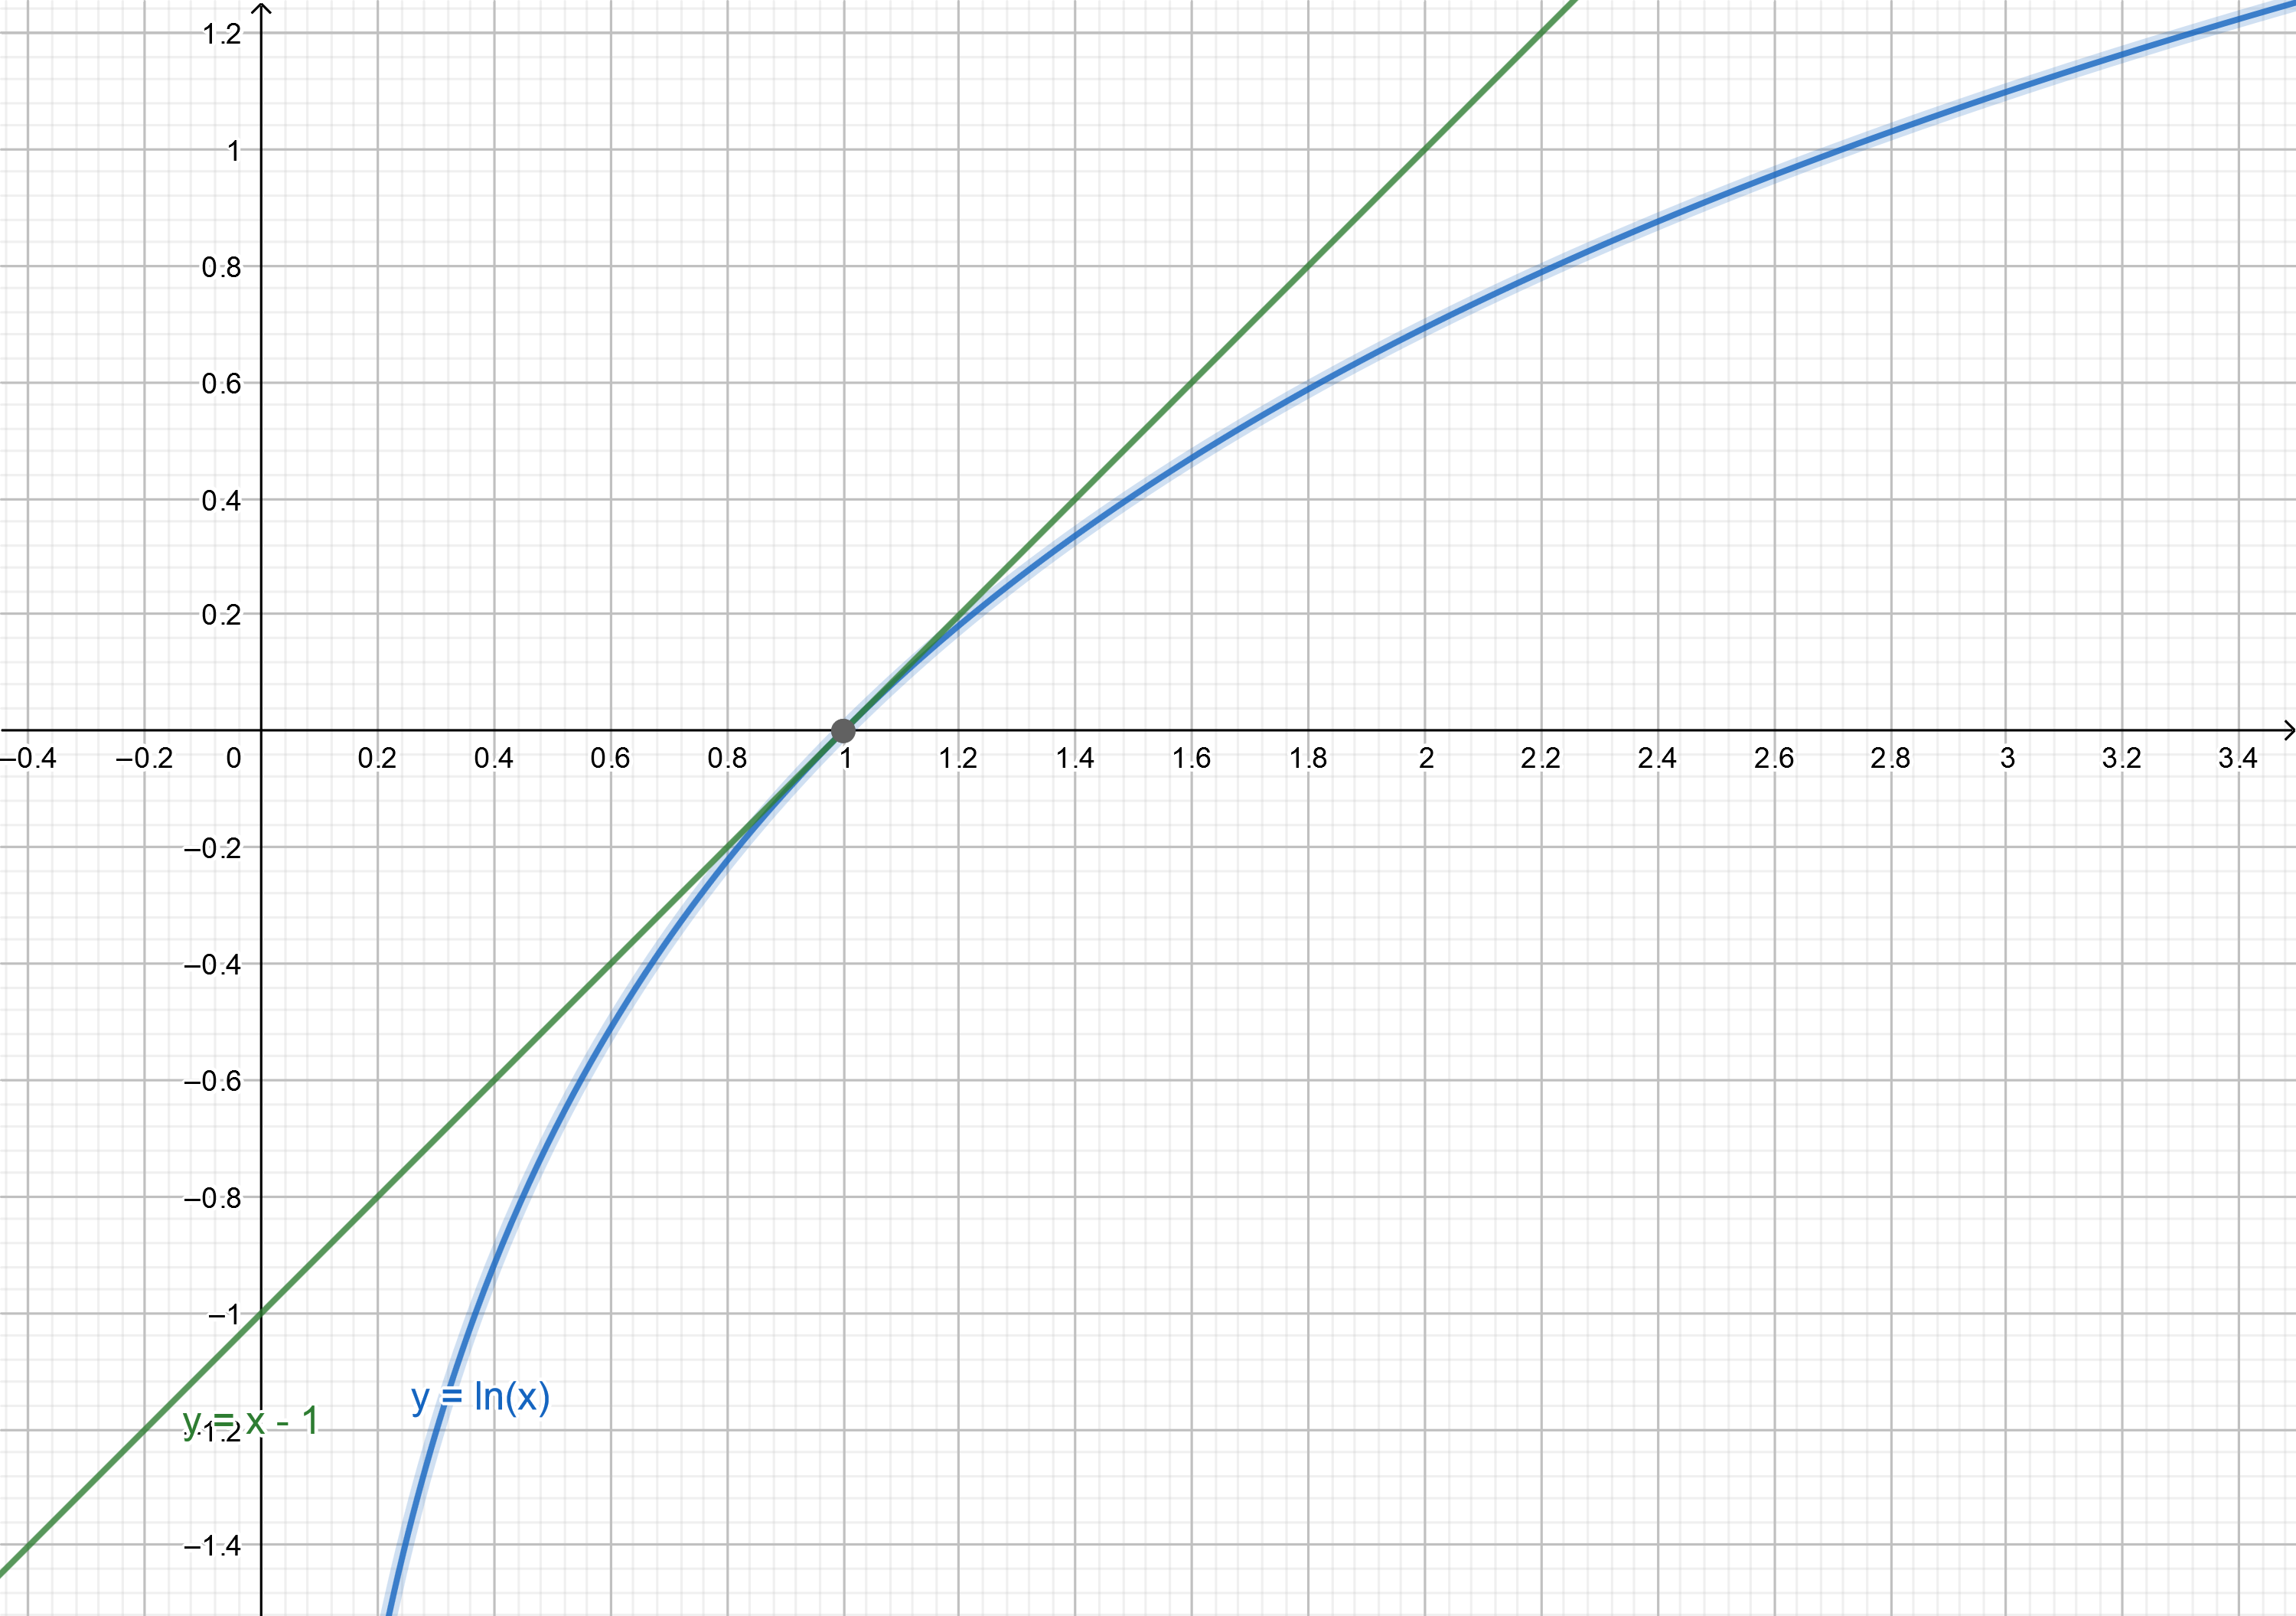
\includegraphics[scale=0.5]{images/sol_kr_3_ip.png}
\end{center}
\end{minipage}
\item[б)] По свойству из предыдущего пункта, 
\[\frac{q(x)}{p(x)}-1\geq\ln \left(\frac{q(x)}{p(x)}\right)\]
\[g(x)-p(x)\geq\ p(x)\ln q(x)-p(x)\ln p(x)\]
\[-p(x)\ln q(x)\geq -p(x)\ln p(x)+p(x)-q(x)\]
Интегрируем:
\begin{align*}-\int^{+\infty}_{-\infty}p(x)\ln q(x) \; dx \geq -\int^{+\infty}_{-\infty}p(x)\ln p(x) \; dx +\\+ \int^{+\infty}_{-\infty}p(x) \; dx - \int^{+\infty}_{-\infty}q(x) \; dx\end{align*}
Поскольку $p(x)$, $q(x)$ – функции плотности, интегрирование каждой из них дает единицу, а значит, последние два слагаемых в сумме равны нулю:
\[-\int^{+\infty}_{-\infty}p(x)\ln q(x) \; dx \geq -\int^{+\infty}_{-\infty}p(x)\ln p(x) \; dx\]
\item[в)] Функция плотности для величины $X \sim \cN(\mu;\sigma^2)$ есть
\[q(x)=\frac{1}{\sqrt{2\pi\sigma^2}}\exp{\left(\frac{-(x-\mu)^2}{2\sigma^2}\right)}\]
\[\ln q(x)=-\frac{1}{2}\ln 2\pi-\ln \sigma-\frac{(x-\mu)^2}{2\sigma^2}\]
\[H(q)=-\int^{+\infty}_{-\infty}q(x)\ln q(x) \; dx\]
\begin{align*}H(q)=\int^{+\infty}_{-\infty}q(x)\left(\frac{1}{2}\ln 2\pi+\ln \sigma+\frac{(x-\mu)^2}{2\sigma^2}\right) \; dx=\\
=\frac{1}{2}\ln 2\pi + \ln \sigma+\int^{+\infty}_{-\infty}q(x)\frac{(x-\mu)^2}{2\sigma^2} \; dx=\\\frac{1}{2}\ln 2\pi + \ln \sigma+\int^{+\infty}_{-\infty}\frac{\left(q(x)x^2-2x\mu q(x)+\mu^2q(x)\right)}{2\sigma^2} \; dx=\\
=\frac{1}{2}\ln 2\pi + \ln \sigma+\frac{1}{2\sigma^2}\left(\E(X^2)-2\mu\E(X)+\mu^2\right)=\\
=\frac{1}{2}\ln 2\pi + \ln \sigma+\frac{1}{2\sigma^2}\left(\sigma^2+\mu^2-2\mu^2+\mu^2\right)=\\=\frac{1}{2}\ln 2\pi + \ln \sigma+\frac{1}{2}\end{align*}
\item[г)] Пусть $Y \sim \cN(\mu_N;\sigma^2_N)$, ее функция плотности равна $q(x)$. Тогда, аналогично пункту в), получаем:
\begin{align*}CE_p(q)=\frac{1}{2}\ln 2\pi + \ln \sigma_N+\\+\int^{+\infty}_{-\infty}\frac{\left(p(x)x^2-2x\mu_N p(x)+\mu^2_Np(x)\right)}{2\sigma^2_N} \; dx=\\
=\frac{1}{2}\ln 2\pi + \ln \sigma_N+\frac{1}{2\sigma^2_N}\left(\sigma^2+\mu^2-2\mu\mu_N+\mu^2_N\right)\end{align*}
\end{enumerate}
\item
\begin{enumerate}
\item[a)] 
\[L=\lambda e^{-\lambda x_1}\lambda e^{-\lambda x_2}\]
\[\ln L=2\ln \lambda-\lambda(x_1+x_2)\]
\[(\ln L)'_\lambda=\frac{2}{\hat{\lambda}}-(x_1+x_2)=0\]
\[\hat{\lambda}=\frac{2}{x_1+x_2}=\frac{1}{15}\]
\item[б)] Пусть $X$ – время обслуживания одного клиента, тогда
\[\P(X>30)=\int^{+\infty}_{30}\lambda e^{-\lambda x} \; dx \Rightarrow\]
\[L=\lambda e^{-\lambda x_1}\lambda e^{-\lambda x_2}\prod^{10}_{i=3}\int^{+\infty}_{30}\lambda e^{-\lambda x_i} \; dx_i\]
\begin{align*}\int^{+\infty}_{30}\lambda e^{-\lambda x} \; dx=-e^{-\lambda x}|^{+\infty}_{30}=e^{-30\lambda}
\end{align*}
\[L=\lambda e^{-\lambda x_1}\lambda e^{-\lambda x_2}\prod^{10}_{i=3}e^{-30\lambda}\]
\[\ln L=2\ln \lambda-\lambda(x_1+x_2)-240\lambda\]
\[(\ln L)'_\lambda=\frac{2}{\hat{\lambda}}-(x_1+x_2)-240=0\]
\[\hat{\lambda}=\frac{1}{135}\]
\item[в)] 
\[\P(X<30)=1-\int^{+\infty}_{30}\lambda e^{-\lambda x} \; dx=1-e^{-30\lambda} \Rightarrow\]
\[L=\prod^{2}_{i=1}(1-e^{-30\lambda})\prod^{10}_{i=3}e^{-30\lambda}\]
\[\ln L=2\ln (1-e^{-30\lambda})-240\lambda\]
\[(\ln L)'_\lambda=\frac{2\cdot30e^{-30\hat{\lambda}}}{1-e^{-30\hat{\lambda}}}-240=0\]
\[\hat{\lambda}\approx0,0074\]
\item[г)]
\[L=\lambda e^{-\lambda x_1}\lambda e^{-\lambda x_2}\prod^{10}_{i=3}e^{-20\lambda}\]
\[\ln L=2\ln \lambda-\lambda(x_1+x_2)-160\lambda\]
\[\hat{\lambda}=\frac{1}{95}\]
\end{enumerate}
\item У всех одинаковые шансы стать Самым Главным, что можно доказать методом математической индукции. Пусть всего метеорологов двое. Тогда, если у них монеты упали одной стороной, они оба выбывают, если разными, то игра продолжается. Если метеорологов трое и у всех монеты выпали одной стороной, то все выходят из игры; если у одного из них выпала решка, а у остальных – орлы, то первый выбывает, получаем ситуацию для двух и т.д.
\item 
\begin{enumerate}
\item[a)] Обозначим количества орлов в соответствующие дни за $S_1$, $S_2$, $S_3$, а количества бросков – за $n_1$, $n_2$, $n_3$. По своим данным Анна может построить оценку $\hat{p}_a=(S_1+S_2)/(n_1+n_2)$, а Белла – $\hat{p}_b=(S_2+S_3)/(n_2+n_3)$. Наша цель – минимизировать по $\alpha$ дисперсию взвешенной оценки:
\[\Var(\hat{p})=\Var(\alpha\hat{p}_a+(1-\alpha)\hat{p}_b)\]
Или явно:
\begin{align*}
    p(1-p)\left(\frac{\alpha}{n_1+n_2}+\frac{(1-\alpha)^2}{n_2+n_3}+\frac{2\alpha(1-\alpha)n_2}{(n_1+n_2)(n_2+n_3)}\right)
\end{align*}
\[\alpha^*=\frac{n_1}{n_1+n_3}\]
Оценки: $\hat{p}_a=0.4$, $\hat{p}_b=0.5$, $\alpha=0.4$, $\hat{p}=0.46$.

\item[б)] Подставим найденную $\alpha^*$ в формулу для дисперсии и получим
\[\frac{n_1n_2+n_2n_3+n_1n_3}{(n_1+n_2)(n_1+n_3)(n_2+n_3)}p(1-p)\]
При наших данных $\hat{\Var}(\hat{p})\approx0.0458$.

\item[в)] Используя стандартную формулу, получим:
\[[\hat{p}-1.96se(\hat{p});\hat{p}+1.96se(\hat{p})],\]
где $\hat{p}=0.46$ и $se(\hat{p})\approx0.214$.
\end{enumerate}
\end{enumerate}

\subsection[2017-2018]{\hyperref[sec:kr_03_ip_2017_2018]{2017-2018}}
\label{sec:sol_kr_03_ip_2017_2018}



\begin{enumerate}
\item
\begin{enumerate}
	\item[а) - в)] См. картинку :)
\begin{figure}[h!]
\centering
\begin{tikzpicture}
\coordinate (e) at (1,0);
\coordinate (X) at (4,3);
\coordinate (hatX) at (4,0);
\coordinate (perpX) at (0,3);
\draw[->] (0,0) -- (e);
\node [below] at (e) {e};
\draw[->] (0,0) -- (X);
\node [right] at (X) {X};
\draw[->] (0,0) -- (hatX);
\node [below] at (hatX) {$\hat{X}$};
\draw[->] (0,0) -- (perpX);
\node [left] at (perpX) {$\hat{X}^{\perp}$};
\draw [dashed] (perpX) -- (X);
\draw [dashed] (hatX) -- (X);
\end{tikzpicture}
\end{figure}
\item[г)] $\hat{X}=e\cdot\bar{X}$

$\lVert \hat{X} \rVert=\sqrt{n}\cdot\bar{X}$

$\hat{X}^{\perp}=X-e\cdot\bar{X}=(X_1-\bar{X}, \dots ,X_n-\bar{X})$

$\lVert\hat{X}^{\perp} \rVert =\sqrt{\sum^n_{i=1}(X_i-\bar{X})^2}$

\item[д)] $ \lVert X \rVert^2=\lVert\hat{X}^{\perp}\rVert^2+\lVert\hat{X}\rVert^2$

$\sum^n_{i=1}X^2_i=\sum^n_{i=1}(X_i-\bar{X})^2+n\bar{X}^2$

\item[е)] t-статистика для построения доверительного интервала для $\mu$ имеет вид:

\begin{align*}
t &= \frac{\bar{X}-\mu}{\sqrt{\bar{\sigma}^2/n}} = \frac{\bar{X}-\mu}{\sqrt{\sum^n_{i=1}(X_i-\bar{X})^2/(n\cdot(n-1))}}\\
& =\sqrt{n-1}\cdot\frac{\sqrt{n}\cdot(\bar{X}-\mu)}{\sqrt{\sum^n_{i=1}(X_i-\bar{X})^2}}=\sqrt{n-1}\cdot\frac{\lVert \hat{X} \rVert-\sqrt{n}\cdot\mu}{\lVert\hat{X}^{\perp} \rVert}
\end{align*}

Заметим, что $\ctg \alpha$ есть отношение прилежащего катета к противолежащему, таким образом, нужный нам угол $\alpha$ образуется между векторами $X$ и $\hat{X}$. Зметим однако, что в нашем случае
\[
t=\sqrt{n-1}\cdot \ctg \alpha=\frac{\lVert\hat{X}\rVert}{\lVert\hat{X}^{\perp}\rVert},
\]
то есть наша статистика подойдёт только для проверки гипотезе о равенстве матожидания нулю.

Замечание. $t=\sqrt{n-1}\cdot \ctg \alpha$ будет t-статистикой только в том случае, если $X_i$ будут н.о.р.с.в. с нормальным распределением, о чём в условие сказано не было.
\end{enumerate}
\item Выпишем функцию правдоподобия для выборки из трёх видов, два из которых совпадают. Первый медведепришелец будет нового вида с вероятностью 1. Вероятность, что вид второго пойманного медведепришельца совпадёт с первмым, составляет $1/n$. После этого нужно поймать медведепришельца нового вида – это произойдёт с вероятностью $(n-1)/n$, и ещё одного нового вида – вероятность этого $(n-2)/n$. Поскольку медведепришелец, вид которого встречается дважды, мог встретить на любой из трёх позиций, функцию правдоподобия необходимо домножить на $C_3^1$. Таким образом, функция правдоподобия имеет вид:
\[
L(n) = C_3^1 \cdot 1 \cdot \frac{1}{n} \cdot \frac{n-1}{n} \cdot \frac{n-2}{n}, n \geq 3.
\]
Максимизируя её, внутри области определения получаем $\hat n = 5$.

Так как количество медведей велико и все они встречаются равновероятно, то $p_{1}=p_{2}=p_{3}=1/n$. Так же из выборки известно, что число видов космомедведей не меньше трёх. Потому $\hat{n} \ge 3$.

Найдите хитрую ошибку в предложенном решении:

$L(n)=\left(\frac{1}{n}\right)^{2} \cdot \frac{1}{n}\cdot\frac{1}{n}=n^{-4}$

$\frac{\partial L(n)}{\partial n} = -4\cdot n^{-5}=0$

Данное уравнение не имеет решений при конечных $n$, но заметим, что при всех $n \ge 3$ выполняется $\frac{\partial L(n)}{\partial n} = -4\cdot n^{-5} < 0$, таким образом максимальное значение находится в граничных точках.

$\lim\limits_{n\to\infty}\frac{1}{n^{-4}}=0 < \frac{1}{3^{-4}}$

Таким образом получаем, что $\hat{n}=3$.

\item \begin{enumerate}
\item $L(p_{1},p_{2})=p_{1}^{150}\cdot p_{2}^{100}\cdot(1-p_{1}-p_{2})^{50}$

$\ell(p_{1},p_{2}) = 150\ln p_{1} +100\ln p_{2}+50\ln (1-p_{1}-p_{2})$

$\begin{cases}
\frac{\partial \ell(p_{1},p_{2})}{\partial p_{1}}= \frac{150}{p_{1}} - \frac{50}{1-p_{1}-p_{2}}=0
\\
\frac{\partial \ell(p_{1},p_{2})}{\partial p_{2}}= \frac{100}{p_{2}} - \frac{50}{1-p_{1}-p_{2}}=0
\end{cases}$

Откуда получаем:

$\begin{cases}
\hat{p}_{1}=1/2
\\
\hat{p}_{2}=1/3
\end{cases}$
\item Найдём, какие значения должны стоять в теоретической ковариационной матрице.
Заметим, что случайная величина найти кальмаромедведя ($X$) или двурога ($Y$) есть бернулевская случайная величина с параметром $p_{1+2}=p_{1}+p_{2}$ и дисперсией $p_{1+2}\cdot(1-p_{1+2})$, но тогда:

$\Var(X + Y)=\Var(X)+\Var(Y)+2\cdot\Cov(X,Y)$

$\Cov(X,Y)=\frac{1}{2}\cdot(\Var(X+Y)-\Var(X)-\Var(Y))=\frac{1}{2}\cdot((p_{1}+p_{2})\cdot(1-p_{1}-p_{2})-p_{1}\cdot(1-p_{1})-p_{2}\cdot(1-p_{2}))=-p_{1}\cdot p_{2}$

Тогда подставляя в теоретическую ковариационную матрицу оценки параметров и домнажая всё на $1/300$, так как $\hat{p}_{1}$ и $\hat{p}_{2}$ являются средними, получим:

\[
\Var(\hat{p})=\frac{1}{n}\begin{pmatrix}
\hat{p}_{1}\cdot(1-\hat{p}_{1}) & -\hat{p}_{1}\cdot\hat{p}_{2}
\\
-\hat{p}_{1}\cdot\hat{p}_{2} & \hat{p}_{1}\cdot(1-\hat{p}_{1})
\end{pmatrix}=\frac{1}{300}\begin{pmatrix}
1/4 &-1/6
\\
-1/6 & 2/9
\end{pmatrix}
\]

\item Для начала, найдём теоретическую дисперсию $\Var(X-Y)$.

\[
\Var(X - Y)=\Var(X)+\Var(Y)-2\cdot\Cov(X,Y)=p_{1}\cdot(1-p_{1})+p_{2}\cdot(1-p_{2})+2\cdot p_{1}\cdot p_{2}
\]

Тогда подставляя оценки для $p_{1}$ и $p_{2}$ и учитывая, что это оценки среднего, получим оценку:

\[
\Var(\hat{p}_{1}-\hat{p}_{2})=1/300\cdot(1/4+2/9+2\cdot1/6)=29/(36\cdot300)
\]

\item Так как выборка достаточно велика, то статистика $\hat{p}_{1}-\hat{p}_{2}$,
являясь средним, будет иметь примерно нормальное распределение, и тогда:

$\frac{\hat{p}_{1}-\hat{p}_{2}-(p_{1}-p_{2})}{\sqrt{\Var(\hat{p}_{1}-\hat{p}_{2})}}\sim \cN(0,1)$

$\hat{p}_{1}-\hat{p}_{2}-z_{1-\frac{\alpha}{2}}\cdot\sqrt{\Var(\hat{p}_{1}-\hat{p}_{2})} \le p_{1}-p_{2} \le \hat{p}_{1}-\hat{p}_{2}-z_{\frac{\alpha}{2}}\cdot\sqrt{\Var(\hat{p}_{1}-\hat{p}_{2})}$
\end{enumerate}
\item \begin{enumerate}
\item $\hat{\alpha}=\bar{X}+\sqrt{\bar{X}+6}=10+\sqrt{10+6}=14$

\item Так как $\bar{X}$ сходится по распределению к нормальному распределению и $\hat{\alpha}=g(\bar{X})$, где $g(\bar{X})$ гладкая по $\bar{X}$ функция при $\bar{X}\ge0$, а также $\bar{X}$ сходится по вероятности к матожиданию, то можно абсолютно спокойно применить дельта-метод. Тогда:

\[
(\alpha-g(\bar{X}))\sim N(0;\sigma^{2}(g'(\E(X_{1})))^{2}/n)
\]

Но так как $\hat{\alpha}$ является состоятельной оценкой, то можно заменить $g'(\E(X_{1}))$ на $g'(\bar{X})$:
\[
g'(\bar{X})=1+\frac{1}{2\cdot\sqrt{\bar{X}+6}}=1+\frac{1}{2\cdot4}=\frac{9}{8}=1.125
\]
и тогда можно построить ассимтотический доверительный интервал:

\begin{align*}
%z_{2.5\%}\le&\frac{\hat{\alpha}-\alpha}{\sqrt{\sigma^{2}\cdot(g'(\bar{X}))^{2}/n}}\le z_{97.5\%} \\
\hat{\alpha}-z_{97.5\%}\cdot\sqrt{\sigma^{2}\cdot(g'(\bar{X}))^{2}/n}\le &\alpha \le
\hat{\alpha}-z_{2.5\%}\cdot\sqrt{\sigma^{2}\cdot(g'(\bar{X}))^{2}/n} \\
16-1.96\cdot2\cdot9/(8\cdot10)\le&\alpha\le 16+1.96\cdot2\cdot9/(8\cdot10) \\
13.559\le&\alpha\le 14.441
\end{align*}
\end{enumerate}
\item \begin{enumerate}
\item Так как не известно точно, кто сколько фотографий сделал, и так как метод оценки не указан,
то воспользуемся методом моментов для построения оценки.

\begin{align*}
N&=\E(\text{«фото Андрея»})+\E(\text{«фото Беллы»}) \\
130&=100\cdot 0.5+p\cdot100 \\
\hat{p}&=0.8
\end{align*}

Так как выборка достаточно велика, то $\frac{\hat{p}-p}{\sqrt{\hat{p}\cdot(1-\hat{p})/W}}\sim \cN(0,1)$

\begin{align*}
\hat{p}-z_{97.5\%}\sqrt{\hat{p}\cdot(1-\hat{p})/W} \le &p \le \hat{p}-z_{2.5\%}\sqrt{\hat{p}\cdot(1-\hat{p})/W} \\
0.8-1.96\cdot\sqrt{0.8\cdot0.2/100}\le &p\le0.8+1.96\cdot\sqrt{0.8\cdot0.2/100} \\
0.72\le &p\le 0.88
\end{align*}

\item Так как неизвестно, кто больше снимков сделал, то рассмотрим два случая: Андрей сделал 60 фото и Белла — 70 фото, Андрей сделал 70 фото и Белла — 60 фото. В каждом случае при помощи метода максимального правдоподобия оценим вероятность $p$, после чего сравним значения функции правдоподобия с оценёнными параметрами для каждого случая.
\begin{align*}
L(p)&=C^{60}_{100}\cdot 0.5^{60}\cdot 0.5^{40}\cdot C^{70}_{100}\cdot p^{70}\cdot(1-p)^{30} \\
\ell(p)&=const+70\ln p+30\ln(1-p) \\
\frac{\partial \ell (p)}{\partial p}&= \frac{70}{p}-\frac{30}{1-p}=0 \\
\hat{p}_1 &= 0.7
\end{align*}

Аналогично для второго случая получим оценку: $\hat{p}_2=0.6$.

Для простоты, будем сравнивать логарифмическии функции правдоподобия $\ell_1(p_1)$ и $\ell_2(p_2)$ и тогда получим:

\begin{align*}
\ell_1(p_1)&=const+70\ln 0.7+30\ln 0.3\approx const-70\cdot0.357-30\cdot 1.204=const-61.11 \\
\ell_2(p_2)&=const+60\ln 0.6+40\ln 0.4\approx const-60\cdot0.511-40\cdot0.916=const-67.3
\end{align*}

Так как $-67.3<-61.11$, то более вероятно, что $\hat{p}=0.7$

Тогда анологично предыдущему пункту получим доверительный интервал:

\begin{align*}
0.7-1.96\cdot\sqrt{0.7\cdot0.3/100}\le &p \le0.7+1.96\cdot\sqrt{0.7\cdot0.3/100} \\
0.61 \le &p \le 0.79
\end{align*}
\end{enumerate}
\end{enumerate}

\thispagestyle{empty}
\section{Решения контрольной номер 4}

\subsection[2018-2019]{\hyperref[sec:kr_04_2018_2019]{2018-2019}}
\label{sec:sol_kr_04_2018_2019}



\subsection[2017-2018]{\hyperref[sec:kr_04_2017_2018]{2017-2018}}
\label{sec:sol_kr_04_2017_2018}

\begin{enumerate}
\item Проверяем следующую гипотезу:
\[
\begin{cases}
H_0: \mu_{D} = 100 \\
H_a: \mu_{D} > 100
\end{cases}
\]
Считаем наблюдаемое значение статистики:
\[
t_{obs} = \frac{\bar X - \mu_{D}}{\frac{\sigma_D}{\sqrt{n_D}}} = \frac{136 - 100}{\frac{55}{\sqrt{40}}} \approx 4.14
\]
При верной $H_0$ $t$-статистика имеет распределение $t_{40 - 1}$, значит, $t_{crit} \approx 1.68$.
Поскольку $t_{crit} > t_{obs}$, основная гипотеза отвергается, $p-value \approx 0$.

\item Проверяем следующую гипотезу:
\[
\begin{cases}
H_0: \sigma^2_D = \sigma^2_T \\
H_a: \sigma^2_D \neq \sigma^2_T
\end{cases}
\]
Считаем наблюдаемое значение статистики:
\[
F_{obs} = \frac{\hat{\sigma}^2_D}{\hat{\sigma}^2_T} = \frac{55^2}{60^2} \approx 0.84
\]
При верной $H_0$ $F$-статистика имеет распределение $F_{40-1, 60-1}$.
Находим критические значения: $F_{left} \approx 0.6$, $F_{right} \approx 1.6$.
Поскольку $F_{left} < F_{obs} < F_{right}$, нет оснований отвергать $H_0$.
\item
\begin{enumerate}
Проверяем гипотезу
\[
\begin{cases}
H_0: \mu_{D} = \mu_{T} \\
H_a: \mu_{D} < \mu_{T}
\end{cases}
\]
\item Когда $n_D$, $n_T$ велики,
\[
\frac{\bar D - \bar T - (\mu_D - \mu_T)}{\sqrt{\frac{\sigma^2_D}{n_D} + \frac{\sigma^2_T}{n_T}}} \stackrel{H_0}{\sim} \cN(0, 1)
\]
Считаем наблюдаемое значение статистики:
\[
z_{obs} = \frac{136 - 139}{\sqrt{\frac{3025}{40} + \frac{3600}{60}}} \approx -0.25
\]
По таблице находим $z_{crit} = -1.28$.
Так как $z_{crit} < z_{obs}$, нет оснований отвергать $H_0$.
\item Когда считаем дисперсии одинаковыми, то:
\[
\hat{\sigma}^2_0 = \frac{\hat{\sigma}^2_D (n_D - 1) + \hat{\sigma}^2_T (n_T - 1)}{n_D + n_T - 2} = \frac{3025 \cdot 39 + 3600 \cdot 59}{30 + 60 - 2} \approx 3371
\]
и
\[
\frac{\bar D - \bar T - (\mu_D - \mu_T)}{\hat{\sigma}^2_0\sqrt{\frac{1}{n_D} + \frac{1}{n_T}}} \stackrel{H_0}{\sim} t_{n_D + n_T - 2}
\]
Считаем наблюдаемое значение статистики:
\[
t_{obs} = \frac{136 - 139}{\sqrt{3371}\sqrt{\frac{1}{40} + \frac{1}{60}}} \approx -0.25
\]
По таблице находим критическое значение: $t_{crit} \approx -1.29$.
Поскольку $t_{crit} < t_{obs}$, нет оснований отвергать $H_0$.
\end{enumerate}
\item
\begin{enumerate}
\item Сначала найдём оценку максимального правдоподобия параметра $\lambda$:
\begin{align*}
L &= \prod_{i=1}^n \lambda e^{-\lambda x_i} = \lambda^n e^{-\lambda \sum_{i=1}^n x_i} \\
\ell &= n \ln \lambda - \lambda \sum_{i=1}^n x_i \\
\frac{\partial \ell}{\partial \lambda} &= \left. \frac{n}{\lambda} \right|_{\lambda = \hat \lambda} = 0 \\
\frac{\partial^2 \ell}{\partial \lambda^2} &= -\frac{n}{\lambda^2} \\
\hat \lambda &= \frac{1}{0.52}
\end{align*}
Так как
\[
\frac{\hat \lambda - \lambda}{\sqrt{\frac{1}{I(\lambda)}}} \stackrel{as}{\sim} \cN(0,1),
\]
доверительный интервал имеет вид
\[
\frac{1}{0.52} - 1.96 \frac{1}{\frac{10}{0.52}} < \lambda < \frac{1}{0.52} + 1.96 \frac{1}{\frac{10}{0.52}}
\]
\item Найдём вероятность того, что наушник проработает без сбоев 45 минут:
\[
g(\lambda) = \P(X > 0.75) = 1 - F(0.75) = e^{-0.75\lambda}
\]
Тогда
\begin{align*}
g(\hat \lambda) &= e^{-0.75 / 0.52} \\
g'(\hat \lambda) &= -0.75 e^{-0.75 / 0.52}
\end{align*}
И доверительный интервал имеет вид:
\[
e^{-0.75 / 0.52} - 1.96 \cdot \frac{0.75 \cdot 0.52}{10} \cdot e^{-0.75 / 0.52} < g(\lambda) < e^{-0.75 / 0.52} + 1.96 \cdot \frac{0.75 \cdot 0.52}{10} \cdot e^{-0.75 / 0.52}
\]
\end{enumerate}
\item Выпишем функцию правдоподобия:
\begin{align*}
L &= p_1^{10} \cdot p_2^{10} \cdot p_3^{15} \cdot p_4^{15} \cdot p_5^{25} \cdot (1 - p_1 - p_2 - p_3 - p_4 - p_5)^{25} \\
\ell &= 10 \ln p_1 + 10 \ln p_2 + 15 \ln p_3 + 15 \ln p_4 + 25 \ln p_5 + 25 \ln (1 - p_1 - p_2 - p_3 - p_4 - p_5)
\end{align*}
Максимизируя логарифмическую функцию правдоподобия по всем параметрам,
получим следующие оценки для неограниченной модели:
\begin{align*}
& \hat p_1 = \hat p_2 = 0.1 \\
& \hat p_3 = \hat p_4 = 0.15 \\
& \hat p_5 = 0.25
\end{align*}
Подставив найденные значения в логарифмическую функцию правдоподобия, получим
\[
\ell_{UR} \approx -172
\]
В ограниченной модели $p_1 = \ldots = p_6 = 1/6$, и значение функции правдоподобия
будет
\[
\ell_R \approx -179
\]
Теперь можно посчитать наблюдаемое значение:
\[
LR = 2(\ell_{UR} - \ell_R) = 2(-172 - (-179)) = 14
\]
Критическое значение $\chi_{0.95, 5} = \approx 11 < 14$, значит, основная гипотеза
отвергается.
\end{enumerate}



\subsection[2016-2017]{\hyperref[sec:kr_04_2016_2017]{2016-2017}}
\label{sec:sol_kr_04_2016_2017}


\begin{enumerate}
\item
\begin{enumerate}
\item $t_{obs} = \frac{\bar X - \mu}{\hat\sigma/\sqrt{n}} = \frac{9.5-10}{0.5/\sqrt{100}} = -10$

В таблице для $t_{0.975;100-1}$ находим $-t_{crit} = -1.66$.

Поскольку $t_{obs} < -t_{crit}$, основная гипотеза отвергается.
\item $p-value \approx 0$
\item $X_1, \ldots, X_{100} \sim \cN(\mu, \sigma^2)$
\item $\gamma_{obs} = \frac{\hat{\sigma}^2}{\sigma^2_0}(n-1) =
\frac{0.5^2}{0.3}(100-1) = 82.5$

В таблице находим нужные значения $\chi^2_{0.975;100-1}$, $\gamma_{crit, r} = 128$
и $\chi^2_{0.025;100-1}$, $\gamma_{crit, l} = 73$.

Так $\gamma_{crit, l} < \gamma_{obs} < \gamma_{crit, r}$, нет оснований отвергать $H_0$.
\end{enumerate}
\item $\hat{p} = \frac{16}{40} = 0.4$, проверять будем двустороннюю гипотезу.

$z_{obs} = \frac{\hat{p} - p}{\sqrt{\hat{p}(1-\hat{p})/n}} =
\frac{0.4-0.5}{\sqrt{0.4\cdot0.6/40}} \approx -1.3$

В таблице нормального распределения находим значение $z_{0.975}$, $z_{crit} = 1.96$.

Так как $\vert z_{obs} \vert < z_{crit}$, нет оснований отвергать $H_0$.
\item
\begin{enumerate}
\item $\hat{\sigma}_0^2 = \frac{\hat{\sigma}_\alpha^2(n_\alpha -1) +
\hat{\sigma}_\beta^2(n_\beta-1)}{n_\alpha + n_\beta-2} = \frac{0.25\cdot19 + 0.36\cdot24}{20+25-2} = 0.31$

$\frac{\bar{X} - \bar{Y}}{\hat{\sigma}_0 \sqrt{\frac{1}{n_\alpha} + \frac{1}{n_\beta}}} \sim t_{n_\alpha + n_\beta-2}$

$t_{obs} = \frac{9.5-9.8}{0.56\sqrt{\frac{1}{20}+ \frac{1}{25}}} = -1.79$

$t_{crit} = 2.02$

Поскольку $\vert t_{obs} \vert < t_{crit}$, нет оснований отвергать $H_0$.
\item Выборки независимы, дисперсии неизвестны, но равны,
$X_1, \ldots, X_{n_\alpha} \sim \cN\left(\mu_X, \sigma^2_X\right)$,
$X_1, \ldots, Y_{n_\beta} \sim \cN\left(\mu_Y, \sigma^2_Y\right)$.
\item $\frac{\hat{\sigma}_\alpha^2}{\hat{\sigma}_\beta^2} \sim F_{n_{\alpha-1}, n_{\beta-1}}$

$F_{obs} = \frac{0.5^2}{0.6^2} \approx 0.69$

$F_{crit, 0.975} = 2.35$, $F_{crit, 0.025} = 0.41$

Поскольку $F_{crit, 0.025} < F_{obs} < F_{crit, 0.975}$, нет оснований отвергать $H_0$.
\end{enumerate}
\item $H_0: p = 0.5$, где $p$ — вероятность того, что бутерброд упадёт маслом вниз.

$\hat{p} = \frac{105}{200} = 0.525$

$z_{obs} = \frac{\hat p - p}{\sqrt{\hat p (1 - \hat p)/n}} = \frac{0.525-0.5}{\sqrt{0.525\cdot0.475/200}} \approx 0.7$

$z_{crit} = 1.96$

Так как $z_{obs} < z_{crit}$, нет оснований отвергать $H_0$.
\item $LR \sim \chi^2_1$, так как в основной гипотезе одно уравнение.
Выпишем функцию правдоподобия и найдём $\hat{\mu}_{ML}$ и $\hat{\nu}_{ML}$.
\begin{align*}
L &= \prod_{i=1}^{100} \frac{1}{\sqrt{2\pi\nu}} \exp\left(-\frac{1}{2} \frac{(x_i-\mu)^2}{\nu} \right) = \frac{1}{(\sqrt{2\pi\nu})^{100}} \exp \left(-\frac{1}{2\nu}\sum_{i=1}^{100} (x_i - \mu)^2 \right) \\
\ell &= -\frac{100}{2}\ln (2\pi) - \frac{100}{2} \ln \nu - \frac{1}{2\nu}\sum_{i=1}^{100} (x_i - \mu)^2 \\
\frac{\partial \ell}{\partial \mu} &= \frac{1}{\nu} \sum_{i=1}^{100} (x_i - \mu) \Rightarrow \hat{\mu}_{ML} = \frac{\sum_{i=1}^{100} x_i}{100} = 0.3 \\
\frac{\partial \ell}{\partial \nu} &= -\frac{100}{2\nu} + \frac{1}{2\nu^2}\sum_{i=1}^{100} (x_i - \mu)^2 \Rightarrow \hat{\nu}_{ML} = 1.37
\end{align*}
Тогда $LR=2(\ell(\hat{\mu}_{ML}, \hat{\nu}_{ML}) - \ell(\hat{\mu}_{ML}, \nu = 1))$ имеет вид:
\[
Q_{obs}= 2 \left(-50 \ln(2\pi) - 50 \ln 1.37 - \frac{1}{2\cdot1.37}\cdot 137 + 50 \ln(2\pi) + 0 + \frac{1}{2} \cdot 137 \right) \approx 5.5
\]
Из таблицы: $Q_{crit} = 3.84$. Поскольку $Q_{obs} > Q_{crit}$, основная гипотеза отвергается.
\end{enumerate}




\subsection[2015-2016]{\hyperref[sec:kr_04_2015_2016]{2015-2016}}
\label{sec:sol_kr_04_2015_2016}

\begin{enumerate}
\item[2.]
\begin{enumerate}
\item
\begin{align*}
  L(x, \lambda) &= \prod_{i=1}^{250} e^{-\lambda} \frac{\lambda^{x_i}}{x_i!} = e^{-250\lambda} \lambda^{\sum_{i=1}^{250} x_i} \prod_{i=1}^{250} \frac{1}{x_i!} \\
  \ell(x, \lambda) &= -250\lambda + \ln\lambda \sum_{i=1}^{250} x_i - \sum_{i=1}^{250} \ln x_i! \\
  \frac{\partial \ell}{\partial \lambda} &= -250 + \frac{1}{\lambda} \sum_{i=1}^{250} x_i \\
  \hat{\lambda}_{ML} &= \bar{X}
\end{align*}
\item $\E\left(\hat{\lambda}_{ML}\right) = \E\left(\bar{X}\right) = \lambda \Rightarrow$ оценка несмещённая.

$\Var\left(\hat{\lambda}_{ML}\right) = \Var\left(\bar{X}\right) = \frac{1}{n^2}\cdot n\Var(X_1) = \frac{\lambda}{n} \to_{n \to \infty} 0 \Rightarrow$ оценка состоятельная.

$\frac{\partial^2 \ell}{\partial \lambda^2} = -\frac{1}{\lambda^2} \sum_{i=1}^{n} x_i$,
$I(\lambda) = - \E\left(-\frac{1}{\lambda^2} \sum_{i=1}^{n} x_i\right) = \frac{n}{\lambda}$.
Так как $\Var\left(\hat{\lambda}_{ML}\right) = \frac{1}{I(\lambda)}$, оценка является эффективной.
\item $\P(X=0) = \frac{\lambda^0 e^{-\lambda}}{0!} = e^{-\lambda} \Rightarrow \widehat{\P(X=0)} = e^{-\hat\lambda} = e^{-\bar{X}}$
\item В данном случае: $g\left(\hat{\lambda}\right) = e^{-\hat\lambda}$, $g'\left(\hat\lambda\right) = -e^{-\hat\lambda}$.
И доверительный интервал имеет вид:
\[
  \left[e^{-\bar{X}} - 1.96 \sqrt{\frac{e^{-2\bar{X}}\bar{X}}{n}}; e^{-\bar{X}} + 1.96 \sqrt{\frac{e^{-2\bar{X}}\bar{X}}{n}} \right]
\]
\end{enumerate}


\item[3.]
\begin{enumerate}
\item $\hat p \stackrel{as.}{\sim}\cN\left(p, \frac{p(1-p)}{n}\right)$

О1Р: лекарство помогает в $80\%$ случаев, но в данной выборке оно помогло менее чем 12 людям.

$\alpha = \P(\text{О1Р}) = \P\left(\hat p < \left. \frac{12}{20} \right| p=0.8 \right) = \P \left(\frac{\hat p - 0.8}{\sqrt{\frac{0.8\cdot0.2}{20}}} < \frac{\frac{12}{20} - 0.8}{\sqrt{\frac{0.8\cdot0.2}{20}}} \right) = 0.0125$
\item О2Р: лекарство помогает в $60\%$ случаев, но $Y \geq 12$.

$\hat p \sim \cN\left(0.6, \frac{0.6\cdot0.4}{20} \right)$

$\beta = \P\left( \hat p \geq \frac{12}{20} \right) = \frac{1}{2}$
\item $\P(Z < a) =0.1$, из таблицы находим, что $a=-1.28$.
\[
a = \frac{\frac{c}{20} - 0.8}{\sqrt{\frac{0.8\cdot0.2}{20}}} = -1.28 \Rightarrow c \approx 13.7
\]
\item $\P(\vert \hat p - p \vert \leq 0.01) \geq 0.95$, будем считать, что $p=0.6$.
\[
\P(\vert \hat p - p \vert \leq 0.01) = \P(-0.01 \leq \hat p - p \leq 0.01) = \P\left(-\frac{0.01}{\sqrt{\frac{0.6\cdot0.4}{n}}} \leq Z \leq \frac{0.01}{\sqrt{\frac{0.6\cdot0.4}{n}}} \right) =0.95
\]
Из таблицы находим
\[
\frac{0.01}{\sqrt{\frac{0.6\cdot0.4}{n}}} = 1.96 \Rightarrow n = \frac{0.6\cdot0.4\cdot1.96^2}{0.01^2}
\]
\end{enumerate}

\item[4.] $H_0: p_{\text{c}} = \frac{1}{7}, p_{\text{л}} = \frac{2}{7}, p_{\text{к}} = \frac{4}{7}$

$Q = \sum_{i=1}^{s=3} \frac{(\nu_i - np_i)^2}{np_i} \sim \chi^2_{s-k-1} = \chi^2_2$

$Q_{obs} = \frac{\left(10-50\frac{1}{7}\right)^2}{50\frac{1}{7}} + \frac{\left(1-50\frac{2}{7}\right)^2}{50\frac{2}{7}} + \frac{\left(39-50\frac{4}{7}\right)^2}{50\frac{4}{7}} = 17.29$

$Q_{crit} = 5.99$, $Q_{crit} < Q_{obs} \Rightarrow$ гипотеза отвергается

\item[5.] $LR \sim \chi^2_1$, так как основная гипотеза содержит одно уравнение

$L(x, \lambda) = \prod_{i=1}^{n=50} \lambda e^{-\lambda x} = \lambda^{50} e^{-\lambda \sum_{i=1}^{n=50} x_i}$

$\ln L (x, \lambda) = 50\ln\lambda - \lambda \sum_{i=1}^{n=50} x_i \to \max_\lambda$

$\frac{\partial \ln L}{\partial \lambda} = \frac{50}{\lambda} - \sum_{i=1}^{n=50} x_i \mid_{\lambda=\hat{\lambda}} = 0 \Rightarrow \hat{\lambda}_{ML} = \frac{1}{\bar{X}} = \frac{10}{11}$

При верной $H_0:  \lambda=1$, тогда $\ln L (\lambda=1) = 50 \ln 1 - 1 \cdot 1.1 \cdot 50 = -55$

При верной $H_1: \lambda=\lambda_{ML}$, тогда $\ln L \left(\lambda=\frac{10}{11}\right) = 50 \ln \frac{10}{11} - \frac{10}{11} \cdot 50 \cdot 1.1 = -54.77$

$LR_{obs} = 2(\ln L (H_1) - \ln(H_0)) = 2(-54.77- (-55)) = 0.46$

$LR_{crit} = 2.71$, $LR_{crit} > LR_{obs} \Rightarrow$ оснований отвергать $H_0$ нет

\item[6.]  Будем проверять гипотезы на уровне значимости $0.05$
\begin{enumerate}
\item $\hat{\sigma}^2_{\text{в}} = 484$, $\hat{\sigma}^2_{\text{р}} = 400$

$\frac{\hat{\sigma}^2_{\text{в}} }{\hat{\sigma}^2_{\text{р}}} \sim F_{21-1 , 19-1}$

$F_{obs} = \frac{484}{400} = 1.21$, $F_{crit, left} = 0.4$, $F_{crit, right} = 2.6  \Rightarrow$ оснований отвергать $H_0$ нет

\item $\hat{\sigma}_0^2 = \frac{484 \cdot (21-1) + 400 \cdot (19-1)}{21 + 19 - 2} \approx 444$

$t_{obs} = \frac{78-67}{\sqrt{444} \sqrt{\frac{1}{21}+ \frac{1}{19}}} \approx 1.8 $

$t_{crit}  \sim t_{21+19-2} = t_{38}$, $t_{crit} = \pm 2.02 \Rightarrow$ нет оснований отвергать $H_0$
\end{enumerate}
\item[7.] $\gamma = \sum_{i=1}^s \sum_{j=1}^m \frac{\left(n_{ij} - \frac{n_{i\cdot}n_{\cdot j}}{n}\right)^2}{\frac{n_{i\cdot}n_{\cdot j}}{n}} \sim \chi^2_{(s-1)(m-1)}$

$\gamma_{obs} = \frac{\left(12-\frac{44\cdot48}{100}\right)^2}{\frac{44\cdot48}{100}} + \frac{\left(36-\frac{56\cdot48}{100}\right)^2}{\frac{56\cdot48}{100}} + \frac{\left(32-\frac{44\cdot52}{100}\right)^2}{\frac{44\cdot52}{100}} + \frac{\left(20-\frac{50\cdot52}{100}\right)^2}{\frac{50\cdot52}{100}} \approx 12$

$\gamma_{crit} = 3.84 \Rightarrow$  гипотеза отвергается

\end{enumerate}



\subsection[2014-2015]{\hyperref[sec:kr_04_2014_2015]{2014-2015}}
\label{sec:sol_kr_04_2014_2015}


\begin{enumerate}

\item[1.] \textbf{Задача для первого потока.}

\begin{enumerate}
\item \begin{align*}
-Z_{\frac{\alpha}{2}}<\frac{\hat{p}-p}{\sqrt{\frac{\hat{p}(1-\hat{p})}{n}}}<Z_{\frac{\alpha}{2}} \\
-1.96<\frac{0.4-p}{\sqrt{\frac{0.4\cdot0.6}{40}}}<1.96 \\
-0.56<p<1.36
\end{align*}

\item $H_0$ не отвергается, так как
\[
-0.56<0.5<1.36
\]

\item $H_0$ отвергается, если $p=0.5$ не лежит в построенном доверительном интервале:
\begin{align*}
0.5\geq0.5Z_{\frac{\alpha}{2}}+0.4 \\
0.2\geq Z_{\frac{\alpha}{2}} \Rightarrow \alpha=0.0456
\end{align*}

\end{enumerate}

\item[1.] \textbf{Задача для второго потока.}
\begin{enumerate}
\item
При верной $H_0: \mu=55$.
Находим $t_{crit} = 1.721$ и $t_{obs} = \frac{51-55}{0.45}= -8.9$, $H_0$ отвергается.

\item
При верной $H_0: \frac{\sigma^2_1}{\sigma^2_2}=1$.
Находим $F_{left} = 0.5$, $F_{right}=2.07$ и $F_{obs} = 2/3$, $H_0$ не отвергается.
\end{enumerate}

\item[2.] \textbf{Задача для первого потока.}

При верной $H_0: \mu_{\alpha}=\mu_{\beta}$.
Находим $t_{crit} = 2.048$ и $t_{obs} =\frac{9.5-9.8}{0.216}= -1.4$, $H_0$ не отвергается.

\item[2.] \textbf{Задача для второго потока.}
\begin{enumerate}
\item
\begin{align*}
\hat{\sigma}^2_1 &= 0.2 \cdot 0.8 = 0.16 \\
\hat{\sigma}^2_2 &= 0.17 \cdot 0.83 = 0.1411
\end{align*}

При верной $H_0: \mu_1=\mu_2$.
Находим $Z_{crit} = 2.58$ и $t_{obs} =\frac{0.2-0.17}{0.06}= 0.5$, $H_0$ не отвергается.
\item
\[
p_{value} = 1 - F(0.5) \approx 1 - 0.6915 = 0.3085
\]
\end{enumerate}

\item[3.]
\begin{align*}
&L(x, \theta) = \theta^{-2n} x^n \exp \left(-\frac{1}{\theta}\sum_ix_i\right) \\
&\ell=\ln(L)=-2n\ln(\theta)+n\ln(x)-\frac{1}{\theta}\sum_ix_i \\
&\ell'_{\theta}=-\frac{2n}{\theta} + \frac{1}{\theta^2}\sum_ix_i \\
&-2n\frac{1}{\hat{\theta}}\sum_ix_i=0 \\
&\hat{\theta}_{ML}=\frac{1}{2}\bar{X} \\
\end{align*}


\item[4.]
Пусть $\ell=\ln(L)$ — логарифмическая функция правдоподобия.
\[
\ell=-\frac{n}{2}\ln(2\pi)-\frac{n}{2}\ln(\nu)-\frac{1}{2\nu}\sum_i(x_i-\bar{x})^2
\]
Известно, что для выборки из нормального распределения
$\hat{\mu}_{ML} = \bar{x} = 0.3$, $\hat{\nu}_{ML} = S^2 = 1.37$, поэтому
\begin{align*}
&\ell_{UR} = -50\ln(2\pi) - 50\ln(1.37)-\frac{137}{2 \cdot 1.37} \\
&\ell_{R} = -50\ln(2\pi) - \frac{137}{2} \\
& LR_{obs}=2\left(-50\ln(2\pi)-50\ln(1.37)-\frac{137}{2\cdot1.37}+50\ln(2\pi)+\frac{137}{2}\right) \approx 12
\end{align*}
При верной $H_0$ $LR\sim\chi^2_1 \Rightarrow LR_{crit}\approx3.8$, основная гипотеза отвергается.

\item[5.] \textbf{Исследовательская задача.}
\begin{enumerate}
\item
Пусть $\ell=\ln(L)$ — логарифмическая функция правдоподобия.
Воспользуемся также тем, что для выборки из нормального распределения
$\hat{\mu}_{ML}=\bar{X}$, $\hat{\nu}_{ML}=S^2$.
\begin{align*}
\ell &= -\frac{n}{2}\ln(2\pi) - \frac{n}{2}\ln(\nu) - \frac{1}{2\nu}\sum^n_{i=1}(x_i-\bar{x})^2 \\
\Var\left(\ell'(\hat{\mu})\right) &= \frac{1}{\nu^2} \Var\left(\sum^n_{i=1}(X_i-\bar{X})\right) = \frac{n}{\nu^2}\Var(X_1) = \frac{n}{\nu} \\
LM &= \frac{\left(\ell'(\hat{\mu}) - \ell'(0)\right)^2}{\Var(\ell'(\hat{\mu}))} = \frac{\left(\frac{1}{\nu}\sum^n_{i=1}(X_i-\bar{X})-\frac{1}{\nu}\sum^n_{i=1}X_i\right)^2}{\frac{n}{\nu}} = \frac{n}{\nu}\bar{X}^2 \\
W &= \frac{(\hat{\mu}-0)^2}{\Var(\hat{\mu})} = \frac{\left(\frac{\sum^n_{i=1}X_i}{n}\right)^2}{\frac{\nu}{n}}=\frac{n}{\nu}\bar{X}^2 \\
\end{align*}
\begin{align*}
LR &= 2\left(-\frac{1}{2\nu}\sum^n_{i=1}(X_i-\bar{X}) + \frac{1}{2\nu}\sum^n_{i=1}X_i\right) = \\
&= \frac{1}{\nu}\left(\sum^n_{i=1}X^2_i-\sum^n_{i=1}X^2_i+2\bar{X} \cdot \sum^n_{i=1}X_i-n\bar{X}^2\right) = \\
&= \frac{1}{\nu} \left(2\bar{X}\cdot n\cdot\bar{X}-n\bar{X}^2\right)=\frac{n}{\nu}\bar{X}^2
\end{align*}
Как видим, $LR=LM=W$.
\item
\end{enumerate}

\item[6.] \textbf{Исследовательская задача.}

\begin{enumerate}

\item
\begin{align*}
\E(X) &= \int^{+\infty}_{0}a^2x^2e^{-ax} dx = -ax^2e^{-ax}\bigg|^{+\infty}_0 + 2\int^{+\infty}_{0}axe^{-ax} dx= \\
&= -2xe^{-ax}\bigg|^{+\infty}_0 + 2\int^{+\infty}_{0}e^{-ax} dx = -\frac{2}{a}e^{-ax}\bigg|^{+\infty}_0=\frac{2}{a} \\
\frac{2}{\hat{a}_{MM}} &= \frac{\sum^{n}_{i=1}x_i}{n} \Rightarrow \hat{a}_{MM}=\frac{2}{3}
\end{align*}

\item
\[
\hat{a}_{MM}=\frac{2}{\bar{X}}
\]

Разложим $\hat{a}_{MM}$ по формуле Тейлора в окрестности точки $\bar{X}=3$:
\begin{align*}
\hat{a}_{MM} &\approx \frac{2}{3} - \frac{2}{9}\left(\bar{X}-3\right) \\
\widehat{\Var}(X) &= \frac{\sum^n_{i=1}(X_i-\bar{X})^2}{n}=\frac{\sum^n_{i=1}X_i^2-2\bar{X}\sum^n_{i=1}X_i+n\bar{X}^2}{n} \\
&= \frac{1000 - 6\cdot300 + 100\cdot9}{100} = 1 \\
\Var\left(\hat{a}_{MM}\right) &\approx \frac{4}{81}\Var\left(\bar{X}\right) = \frac{4\cdot100}{81\cdot100^2} \Var(X)\Rightarrow \widehat{\Var}\left(\hat{a}_{MM}\right) = \frac{4}{8100}
\end{align*}
\item
\begin{align*}
-t_{\frac{\alpha}{2};n-1}<\frac{\bar{X}-\mu}{\frac{\hat{\sigma}}{\sqrt{n}}}<t_{\frac{\alpha}{2};n-1} \\
-1.98<\frac{3-\mu}{\frac{1}{10}}<1.98
\end{align*}
Воспользуемся тем, что $\mu=\frac{2}{a}$:

\begin{align*}
-1.98<\frac{3-\frac{2}{a}}{\frac{1}{10}}<1.98 \\
-0.198<3-\frac{2}{a}<0.198 \\
0.63<a<0.71
\end{align*}

\end{enumerate}
\end{enumerate}


\subsection[2009-2010]{\hyperref[sec:kr_04_2009_2010]{2009-2010}}
\label{sec:sol_kr_04_2009_2010}

% % !TEX root = ../probability_hse_exams.tex
\thispagestyle{empty}
\section{Решения контрольной номер 4. ИП}




\subsection[2018-2019]{\hyperref[sec:kr_04_ip_2018_2019]{2018-2019}}
\label{sec:sol_kr_04_ip_2018_2019}


\subsection[2017-2018]{\hyperref[sec:kr_04_ip_2017_2018]{2017-2018}}
\label{sec:sol_kr_04_ip_2017_2018}
% !TEX root = ../probability_hse_exams.tex
\thispagestyle{empty}
\section{Решения финальных экзаменов}

\subsection[2018-2019]{\hyperref[sec:final_exam_2018_2019]{2018-2019}}
\label{sec:sol_final_exam_2018_2019}

CACAE ACCBA BDEBA DDBEB ECEBC EAEAD

\subsection[2017-2018]{\hyperref[sec:final_exam_2017_2018]{2017-2018}}
\label{sec:sol_final_exam_2017_2018}

Здесь табличка с ответами



\end{document}
